\documentclass[10pt,a4paper]{article}
\usepackage[a4paper,hmargin=1.4cm,top=1.2cm,bottom=1.2cm]{geometry}
\usepackage[T1]{fontenc}
\usepackage{lmodern}
\usepackage{microtype,amsmath,amssymb,booktabs,graphicx,xcolor,enumitem,caption,array}
\usepackage[colorlinks,linkcolor=blue!50!black,urlcolor=blue!50!black]{hyperref}
\captionsetup{font=small,labelfont=bf}
\setlist{itemsep=1pt,topsep=2pt,leftmargin=*}
\setlength{\parskip}{3pt}
\setlength{\parindent}{0pt}
\emergencystretch=3em
\newcommand{\atol}{\mathrm{atol}}
\newcommand{\rtol}{\mathrm{rtol}}
\newcommand{\Eth}{E_{\rm th}}
\newcommand{\Eeq}{E_{\rm eq}}

\title{Integrator and Tolerance Bench on Small Mode Networks}
\date{21 October 2026}

\begin{document}
\maketitle
\vspace{-1.5em}

\section*{In short}
No run is singled out as a reference here; every statement compares runs with each other. $\Delta$ means the detuning throughout.
\begin{enumerate}
    \item \textbf{The absolute tolerance, not the integrator, causes the disagreements seen in earlier sweeps.}
        \begin{itemize}
            \item At $\atol=10^{-40}$ (the sweep default so far), bursts happen at different times for different integrators on four of the nine networks (and on \texttt{2p\_M2.0T\_eth}, see item 5).
            \item At $\atol=10^{-300}$, the five integrators give the same curves on eight of the nine networks.
        \end{itemize}
    \item \textbf{$\atol=0$ (pure relative error control) reproduces $\atol=10^{-300}$ exactly wherever it finishes.} It does not finish on \texttt{2p\_M2.0T\_eth}, where an amplitude decays below the smallest normal double: rk8pd crawls into the wall-time limit there, and CVODE stops with ``too much accuracy requested''.
    \item \textbf{rk8pd is the cheapest integrator.} At $\atol=10^{-300}$, measured against rk8pd (medians over the networks):
        \begin{itemize}
            \item BDF takes $11.6\times$ the steps and $5.8\times$ the wall time;
            \item Adams takes $5.2\times$ the steps and $2.9\times$ the wall time.
        \end{itemize}
    \item \textbf{BDF-Krylov (GMRES with a banded finite-difference preconditioner) gives the same curves as BDF with the analytic Jacobian, but it is not faster at these sizes ($\le6$ modes).} Preconditioner band 3 and the full band behave the same.
    \item \textbf{\texttt{2p\_M2.0T\_eth} disagrees between runs at every setting.} One daughter's exact dip ($E\sim10^{-3600}$) is far below what a double can hold.
    \item \textbf{Proposal for the sweep:} rk8pd, $\rtol=10^{-8}$, $\atol=10^{-300}$. The decisions are listed in \S\ref{sec:decisions}.
\end{enumerate}

\section{Setup}

\subsection{Equations and notation}
Each mode $a$ has a slow complex amplitude $A_a(t)$, with $t$ in seconds. For a triplet $(a,b,c)$ with $b\ne c$, mode $a$ obeys
\begin{equation}
    \dot A_a = -\gamma_a A_a + 2i\,\omega_a\,\kappa_{abc}\,A_b^*A_c^*\,e^{i\Delta_{abc}t},
    \qquad \Delta_{abc}=\omega_a+\omega_b+\omega_c .
\end{equation}
Each triplet that contains $a$ adds such a term. A self-coupled pair ($b=c$) has the coefficient $1$ instead of $2$ in the parent's equation. The symbols are:
\begin{itemize}
    \item $\omega_a$: the mode frequency, signed by generation. Generation 0 (the parents) has $-|\omega|$; generation 1 (the daughters) has $+|\omega|$.
    \item $\Delta_{abc}$: the detuning of the triplet. With the signs above it is small for a parent $\to$ daughter + daughter triplet. It is fixed by the network: it is the same in every run of a given network.
    \item $\gamma_a$: the linear damping rate, in s$^{-1}$. $\gamma_a<0$ means the mode is driven (the parents); $\gamma_a>0$ means it is damped.
    \item $\kappa_{abc}$: the three-mode coupling coefficient.
    \item $E_a=|A_a|^2$: the mode energy, in units of $E_\star$.
    \item $\Eth$: a parent's parametric threshold energy for its selecting pair (Weinberg+12, eq.~50).
    \item $\Eeq$: the three-mode equilibrium energy (MW25, eq.~6). It is absent when the triplet has no stable equilibrium.
\end{itemize}
The integrators advance the real vector $y=(\operatorname{Re}A_0,\operatorname{Im}A_0,\dots,\operatorname{Re}A_{n-1},\operatorname{Im}A_{n-1})$ of length $2n$, where $n$ is the number of modes.

\subsection{Error control and the energy floor}
\textbf{The step test.} Both libraries accept a step when the local error estimate $e_i$ of each component $y_i$ satisfies
\begin{equation}
    |e_i| \lesssim \atol + \rtol\,|y_i| .
\end{equation}
GSL applies this test to each component separately. CVODE applies it through a weighted root-mean-square norm, with weights $1/(\rtol|y_i|+\atol)$.

\textbf{The floor.}
\begin{itemize}
    \item When $|y_i|\gg\atol/\rtol$, the error control is relative. Below that, it is absolute: the component is held only to about $\pm\atol$.
    \item So a decaying mode is not followed below $|A|\sim\atol$, i.e.\ $E\sim\atol^2$. Each integrator leaves the mode at its own level near this floor.
    \item When the mode later grows back at rate $\sigma$, it needs a time of about $\ln(\Eth/E_{\rm floor})/(2\sigma)$ to reach threshold. A floor that differs by tens of decades therefore moves the next burst.
\end{itemize}

\textbf{Why $\atol=0$ is fragile.}
\begin{itemize}
    \item $\atol=0$ removes the floor but asks for relative accuracy at every magnitude.
    \item Doubles below $2.2\times10^{-308}$ are subnormal and carry fewer significant digits. Once an amplitude reaches that range ($E\lesssim5\times10^{-616}$), the requested accuracy cannot be met: rk8pd's step size collapses, and CVODE stops.
    \item A mode decaying freely from $E=10^{-18}$ reaches that range after about $690/\gamma$.
\end{itemize}

\begin{table}[h]
    \centering\small
    \caption{The absolute tolerances tested and the energy floor each one implies.}
    \begin{tabular}{@{}lll@{}}
        \toprule
        $\atol$ & floor $E\sim\atol^2$ & note \\
        \midrule
        $10^{-40}$ & $10^{-80}$ & sweep default so far \\
        $10^{-150}$ & $10^{-300}$ & \\
        $10^{-300}$ & $10^{-600}$ & near the double-precision limit for $A$ \\
        $0$ & none & pure relative control; fails once an $A$ becomes subnormal ($E\lesssim5\times10^{-616}$) \\
        \bottomrule
    \end{tabular}
\end{table}

\subsection{Integrators}
\begin{table}[h]
    \centering\small
    \caption{The five integrator configurations. GSL 2.8; CVODE from SUNDIALS 7.9.0 (the cluster has 7.1.1).}
    \begin{tabular}{@{}>{\raggedright}p{2.8cm}>{\raggedright}p{5.9cm}>{\raggedright\arraybackslash}p{8.5cm}@{}}
        \toprule
        label & method & linear algebra \\
        \midrule
        rk8pd & GSL \texttt{rk8pd}: explicit embedded Runge--Kutta Prince--Dormand 8(9) & none \\
        BDF, dense analytic Jacobian & CVODE BDF, orders 1--5, Newton iteration, stability-limit detection & dense LU on the hand-written Jacobian \\
        BDF-Krylov, band full & as BDF & GMRES (SPGMR, Krylov dimension 5), with Jacobian--vector products by finite differences. Left preconditioner CVBANDPRE: a banded finite-difference Jacobian of half-bandwidth $2n-1$ (the whole matrix) \\
        BDF-Krylov, band 3 & as BDF & as above, half-bandwidth 3 \\
        Adams, fixed point & CVODE Adams--Moulton, orders 1--12, fixed-point iteration & none \\
        \bottomrule
    \end{tabular}
\end{table}

\textbf{Restarts.}
\begin{itemize}
    \item CVODE is re-initialised (\texttt{CVodeReInit}) at each of the 4000 outputs, with its local time set back to 0. GSL likewise restarts its local time in each output interval.
    \item The phase factor $e^{i\Delta t}$ at the restart time is carried along as a constant.
    \item This keeps $t$ small inside the exponential. Otherwise rounding of $t\approx10^{13}$\,s would add phase noise of order $\Delta\,\varepsilon\,t$, where $\varepsilon$ is the machine epsilon.
    \item The restarts cost almost nothing. BDF at $\atol=10^{-40}$ on \texttt{1p2d\_M1.7\_eth} took 6.39\,M steps with them, against 6.92\,M steps in the earlier cluster run without them.
\end{itemize}

\subsection{Runs}
\begin{itemize}
    \item \textbf{Networks.} Nine networks (Table~\ref{tab:nets}), made by \texttt{network\_build} with $N=1$ or 4, cut 0.15 and closure 0.005.
        \begin{itemize}
            \item The name prefix gives the shape: \texttt{1p2d} is one parent with one daughter pair, \texttt{1p4d} is one parent with two pairs, and \texttt{2p} is two parents with one pair each.
            \item The suffix gives the pair-ranking rule.
        \end{itemize}
    \item \textbf{Initial state.} Parents start at $|A|=10^{-6}$ ($E=10^{-12}$) and daughters at $|A|=10^{-9}$ ($E=10^{-18}$). The phases are random, with seed 1.
    \item \textbf{Time span.} $t_{\rm end}=10^{13}$\,s, with 4000 equally spaced outputs. A run stops early, as a runaway, once $\sum_a E_a>10^{-2}$.
    \item \textbf{Tolerances.}
        \begin{itemize}
            \item All five integrators: $\rtol=10^{-8}$, with $\atol\in\{10^{-40},10^{-150},10^{-300},0\}$.
            \item rk8pd also ran at $\rtol=10^{-10}$ ($\atol=0$ and $10^{-40}$ only) and at $\rtol=10^{-12}$ (all four $\atol$); see Appendix~\ref{app:rk8pd}.
        \end{itemize}
    \item \textbf{Wall-time limits.}
        \begin{itemize}
            \item \texttt{network\_run --max-seconds 900}. It is checked only between outputs, so it cannot stop a run that stalls inside one output interval.
            \item The bench scripts also kill a run after 600\,s (rk8pd) or 1000\,s (CVODE).
        \end{itemize}
    \item \textbf{Machine.} A laptop running up to six runs at once. Wall times are good to about a factor of 2; step counts are exact.
\end{itemize}

\textbf{Stop codes.}
\begin{itemize}
    \item \texttt{end}: reached $t_{\rm end}$.
    \item \texttt{runaway}: crossed $\sum E=10^{-2}$.
    \item \texttt{failed}: CVODE returned an error. All four failures here are ``too much accuracy requested''.
    \item \texttt{wall}: stopped by the 900\,s limit.
    \item \texttt{stalled}: killed by the bench script's timeout; no output was written.
\end{itemize}

\subsection{Table columns}\label{sec:columns}
The integrator advances in time steps whose length $h$ it picks itself. The basic unit of work is one evaluation of the right-hand side $f(t,y)=\dot y$, i.e.\ $\dot A$ for every mode. The examples are \texttt{1p2d\_M1.7\_eth} at $\atol=10^{-300}$ (\S\ref{net:1p2d_M1.7_eth}). ``--'' means the column does not apply to that integrator.

\begin{description}[style=nextline,leftmargin=1.2cm,itemsep=3pt]
    \item[steps] Accepted steps: how many times the solution was advanced in time.
        \begin{itemize}
            \item rk8pd took 1.13\,M.
            \item BDF took 13.78\,M. It is lower order, so it needs shorter steps for the same accuracy.
        \end{itemize}

    \item[rejected] Steps that were tried, thrown away and retried with a shorter step. They cost work but do not advance the solution.
        \begin{itemize}
            \item rk8pd rejects a step when its error estimate exceeds $\atol+\rtol|y_i|$.
            \item CVODE also rejects a step when the iteration that solves for the new state (see NL it.) fails to converge.
        \end{itemize}

    \item[RHS] Right-hand-side evaluations, counted inside our $f$, so everything that calls it is included. This is the fairest cost measure that does not depend on the machine.
        \begin{itemize}
            \item \textbf{rk8pd:} about 12 per attempted step (13 stages, the first one reused). Here $14.65\,\mathrm M \approx 12\times(1.13\,\mathrm M + 0.13\,\mathrm M)$.
            \item \textbf{BDF and Adams:} one per nonlinear iteration, so RHS $\approx$ NL it.
            \item \textbf{BDF-Krylov:} one per nonlinear iteration, plus one per GMRES iteration, plus about $2n$ per preconditioner build. Here $29.86\,\mathrm M \approx 14.47\,\mathrm M + 13.98\,\mathrm M + 6\times234.6\,\mathrm k$, which is about twice dense BDF's count for the same number of steps.
        \end{itemize}

    \item[Jac.] Jacobian evaluations. The Jacobian is the $2n\times2n$ matrix $J=\partial f/\partial y$.
        \begin{itemize}
            \item \textbf{BDF:} computed from the hand-written formula. CVODE reuses $J$ across many steps and recomputes it only when its iteration starts to converge slowly: 241\,k Jacobians for 13.78\,M steps.
            \item \textbf{BDF-Krylov:} CVBANDPRE's banded finite-difference approximation of $J$, used as the preconditioner.
            \item \textbf{rk8pd and Adams:} use no Jacobian.
        \end{itemize}

    \item[NL it.] Nonlinear iterations. BDF and Adams are implicit: the new state appears on both sides of the update,
        \[
            y_{\rm new} = (\text{terms from earlier steps}) + h\,\beta\, f(t_{\rm new}, y_{\rm new}),
        \]
        with $\beta$ a fixed coefficient of the method. The integrator therefore solves for $y_{\rm new}$ iteratively.
        \begin{itemize}
            \item \textbf{BDF:} Newton iteration, which uses $J$.
            \item \textbf{Adams:} fixed-point iteration (put the current guess into $f$ and repeat), which needs no $J$.
            \item Here it takes about one iteration per step: 14.74\,M iterations for 13.78\,M BDF steps.
            \item \textbf{rk8pd:} explicit, so it has none.
        \end{itemize}

    \item[lin. it.] GMRES iterations; BDF-Krylov only. Each Newton iteration solves a linear system with the matrix $I-h\beta J$.
        \begin{itemize}
            \item \textbf{Dense BDF:} solves it directly by LU factorisation, so there are no iterations to count.
            \item \textbf{BDF-Krylov:} solves it iteratively with GMRES. Each GMRES iteration needs one product $Jv$, which is approximated with one extra right-hand-side evaluation.
        \end{itemize}

    \item[wall {[s]}] Elapsed clock time of the integration, in seconds. Up to six runs shared the laptop, so it is good only to about a factor of 2. Use steps and RHS for exact comparisons.
\end{description}

\section{Overview}

\begin{table}[h]
    \centering\footnotesize
    \caption{The networks. Each name links to its page.}
    \label{tab:nets}
    \begin{tabular}{@{}llrrrl@{}}
\toprule
network & model & modes & parents & triplets & rule \\
\midrule
\hyperref[net:1p2d_M1.7_eth]{\texttt{1p2d\_M1.7\_eth}} & \texttt{dsct\_M1.7\_T7750} & 3 & 1 & 1 & eth \\
\hyperref[net:1p2d_M2.0T_eth]{\texttt{1p2d\_M2.0T\_eth}} & \texttt{dsct\_M2.0\_T7696} & 3 & 1 & 1 & eth \\
\hyperref[net:1p2d_M2.0_dgamma]{\texttt{1p2d\_M2.0\_dgamma}} & \texttt{dsct\_M2.0} & 3 & 1 & 1 & dgamma \\
\hyperref[net:1p4d_M1.7_eth]{\texttt{1p4d\_M1.7\_eth}} & \texttt{dsct\_M1.7\_T7750} & 5 & 1 & 2 & eth \\
\hyperref[net:1p4d_M2.0T_eth]{\texttt{1p4d\_M2.0T\_eth}} & \texttt{dsct\_M2.0\_T7696} & 5 & 1 & 2 & eth \\
\hyperref[net:1p4d_M2.0_eth]{\texttt{1p4d\_M2.0\_eth}} & \texttt{dsct\_M2.0} & 5 & 1 & 2 & eth \\
\hyperref[net:2p_M1.7_eth]{\texttt{2p\_M1.7\_eth}} & \texttt{dsct\_M1.7\_T7750} & 6 & 2 & 2 & eth \\
\hyperref[net:2p_M2.0T_eth]{\texttt{2p\_M2.0T\_eth}} & \texttt{dsct\_M2.0\_T7696} & 5 & 2 & 2 & eth \\
\hyperref[net:2p_M2.0_eeq]{\texttt{2p\_M2.0\_eeq}} & \texttt{dsct\_M2.0} & 6 & 2 & 2 & eeq \\
\bottomrule
\end{tabular}
\end{table}

\begin{figure}[p]
    \centering
    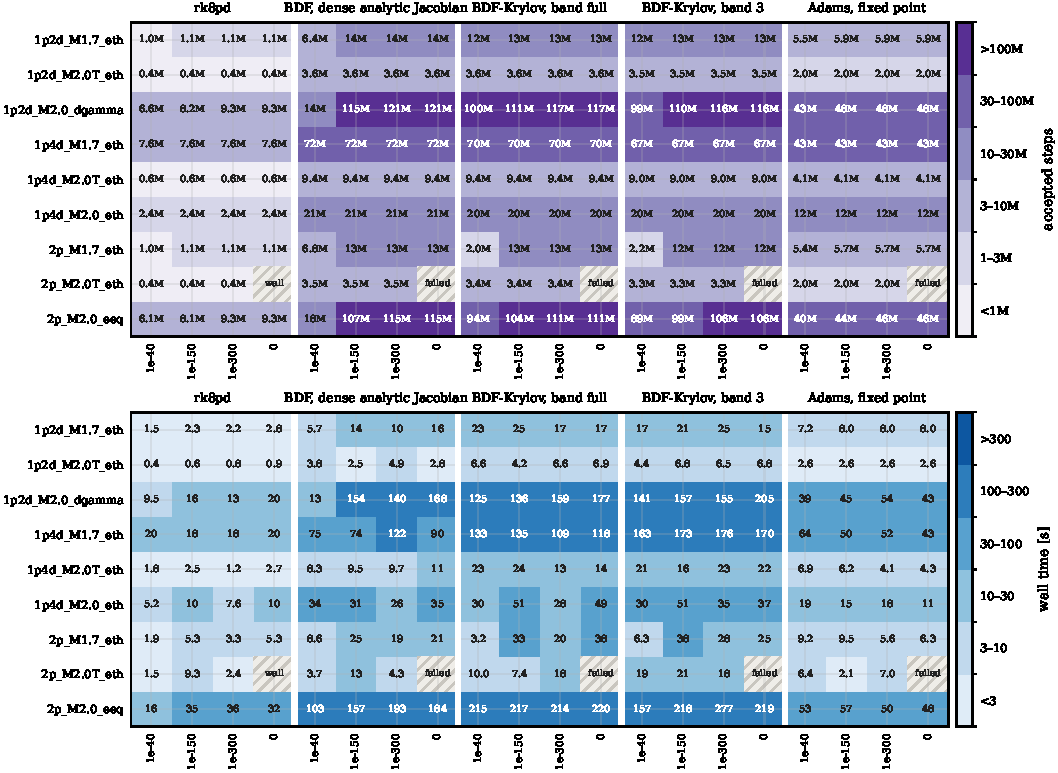
\includegraphics[width=\textwidth]{figs/maps.pdf}
    \caption{Cost of every network $\times$ (integrator, $\atol$) at $\rtol=10^{-8}$. \textbf{Top:} accepted steps. \textbf{Bottom:} wall time. Hatched cells stopped early (\texttt{failed}, \texttt{wall} or \texttt{stalled}).}
    \label{fig:maps}
\end{figure}

\begin{table}[h]
    \centering\footnotesize
    \caption{Cost of each (integrator, $\atol$) pair over the nine networks at $\rtol=10^{-8}$. The ratios are medians over the networks where both this run and rk8pd at the same $\atol$ finished. $^*$ Sum over the finished runs only.}
    \label{tab:summary}
    \begin{tabular}{@{}llrrrrr@{}}
\toprule
integrator & atol & stopped early & steps / rk8pd & wall / rk8pd & $\sum$ steps & $\sum$ wall [s] \\
 & & (of 9) & median & median & & \\
\midrule
rk8pd & $10^{-40}$ & 0 & 1.00 & 1.00 & 26.03\,M & 58 \\
 & $10^{-150}$ & 0 & 1.00 & 1.00 & 29.99\,M & 99 \\
 & $10^{-300}$ & 0 & 1.00 & 1.00 & 32.16\,M & 85 \\
 & $0$ & 1 & 1.00 & 1.00 & 31.77\,M$^*$ & 94$^*$ \\
\addlinespace[2pt]
BDF, dense analytic Jacobian & $10^{-40}$ & 0 & 8.71 & 4.44 & 155.79\,M & 255 \\
 & $10^{-150}$ & 0 & 11.60 & 4.21 & 359.03\,M & 480 \\
 & $10^{-300}$ & 0 & 11.59 & 5.81 & 372.31\,M & 530 \\
 & $0$ & 1 & 11.91 & 4.31 & 368.85\,M$^*$ & 528$^*$ \\
\addlinespace[2pt]
BDF-Krylov, band full & $10^{-40}$ & 0 & 9.22 & 13.10 & 314.58\,M & 569 \\
 & $10^{-150}$ & 0 & 11.30 & 7.07 & 347.45\,M & 633 \\
 & $10^{-300}$ & 0 & 11.30 & 7.62 & 359.96\,M & 585 \\
 & $0$ & 1 & 11.62 & 6.39 & 356.55\,M$^*$ & 639$^*$ \\
\addlinespace[2pt]
BDF-Krylov, band 3 & $10^{-40}$ & 0 & 9.20 & 11.31 & 304.81\,M & 557 \\
 & $10^{-150}$ & 0 & 10.98 & 7.16 & 337.80\,M & 701 \\
 & $10^{-300}$ & 0 & 10.98 & 8.51 & 350.54\,M & 744 \\
 & $0$ & 1 & 11.23 & 7.05 & 347.22\,M$^*$ & 699$^*$ \\
\addlinespace[2pt]
Adams, fixed point & $10^{-40}$ & 0 & 5.64 & 4.14 & 157.31\,M & 208 \\
 & $10^{-150}$ & 0 & 5.28 & 2.45 & 165.80\,M & 196 \\
 & $10^{-300}$ & 0 & 5.21 & 2.88 & 168.85\,M & 202 \\
 & $0$ & 1 & 5.21 & 1.86 & 166.85\,M$^*$ & 167$^*$ \\
\bottomrule
\end{tabular}
\end{table}

\subsection{Findings}
\begin{enumerate}
    \item \textbf{atol, not the integrator, sets the curves.}
        \begin{itemize}
            \item At $\atol=10^{-300}$ and at $\atol=0$, the five integrators agree to within 0.25 decades in $E$ at every output where $E>10^{-34}$ (the plots' lower edge) on eight networks; the exception is \texttt{2p\_M2.0T\_eth}. By eye, their plots are the same.
            \item At $\atol=10^{-40}$, bursts move on four networks: \texttt{1p2d\_M1.7\_eth}, \texttt{1p2d\_M2.0\_dgamma}, \texttt{2p\_M1.7\_eth} and \texttt{2p\_M2.0\_eeq}.
                \begin{itemize}
                    \item The bursts move between integrators.
                    \item Each integrator's bursts also move relative to its own $\atol=10^{-300}$ run.
                    \item The cause is that each integrator leaves the decaying daughters at a different level around the $10^{-80}$ floor, and the next burst follows from that level.
                \end{itemize}
            \item This explains the earlier rk8pd--BDF disagreement on \texttt{1p2d\_M1.7\_eth}: both were run at $\atol=10^{-40}$.
            \item $\atol=10^{-150}$ removes the differences on the two M1.7 networks, but not on \texttt{dgamma} and \texttt{eeq}.
        \end{itemize}
    \item \textbf{$\atol=10^{-300}$ and $\atol=0$ give identical curves for every integrator, wherever $\atol=0$ finishes.} $\atol=0$ does not finish on \texttt{2p\_M2.0T\_eth}:
        \begin{itemize}
            \item rk8pd crawls to the wall-time limit at $5.1\times10^{11}$\,s, after 50\,M steps;
            \item all CVODE configurations fail at $4.85\times10^{11}$\,s.
        \end{itemize}
    \item \textbf{rk8pd is the cheapest integrator.} At every $\atol$ it takes the fewest steps on every network. It is also the fastest by wall time, with one exception: Adams on \texttt{2p\_M2.0T\_eth} at $10^{-150}$, which is within the timing noise.
    \item \textbf{BDF-Krylov gives no gain at these sizes.}
        \begin{itemize}
            \item The finite-difference Jacobian is as good as the hand-written one: the curves are the same, and BDF-Krylov takes 1--8\,\% fewer steps than dense BDF.
            \item Each step costs more. The median wall time is $7.6$--$8.5\times$ rk8pd's, against $5.8\times$ for dense BDF.
            \item Band 3 and the full band behave the same.
            \item With $2n\le12$ unknowns, a dense LU solve is trivial. A Krylov solver is expected to pay off only for hundreds of modes; this was not tested.
        \end{itemize}
    \item \textbf{$\rtol=10^{-8}$ is enough for rk8pd} (Appendix~\ref{app:rk8pd}). At $\atol=10^{-300}$, rk8pd at $\rtol=10^{-8}$ and at $\rtol=10^{-12}$ agree to within 0.01 decades on every network except \texttt{2p\_M2.0T\_eth}.
    \item \textbf{\texttt{2p\_M2.0T\_eth} cannot be converged in double precision.}
        \begin{itemize}
            \item The daughter (14,$-48$) is fed by parent (2,$-3$) through a self-coupled pair. In exact arithmetic it decays to $E\sim10^{-3600}$ by $3\times10^{12}$\,s.
            \item Its regrowth time is set by whichever floor a run has. So the runs disagree with each other at every $\atol$, at every $\rtol$, and for every integrator.
            \item Any network whose exact dips go below about $10^{-600}$ will behave like this.
        \end{itemize}
\end{enumerate}

\section{Decisions}\label{sec:decisions}
\begin{enumerate}
    \item \textbf{Sweep integrator and tolerances.}
        \begin{enumerate}
            \item[(a)] \emph{rk8pd, $\rtol=10^{-8}$, $\atol=10^{-300}$ (proposed).}
                \begin{itemize}
                    \item The same curves as every other integrator and as $\atol=0$.
                    \item The cheapest option, and it never stalled.
                    \item Requires changing \texttt{RUN\_ARGS} in \texttt{network\_sweep.sh} from \texttt{--atol 1e-40}.
                \end{itemize}
            \item[(b)] \emph{$\atol=0$.} The same curves, but it fails on networks with very deep dips. A stalled run also defeats \texttt{--max-seconds}.
            \item[(c)] \emph{A physical floor, $\atol=\sqrt{E_{\min}}$} (the ``$E_{\rm min,crash}$'' idea).
                \begin{itemize}
                    \item This is a choice of physics, not of numerics.
                    \item The \texttt{dgamma} and \texttt{eeq} networks show that a floor of $E_{\min}\gtrsim10^{-300}$ already moves bursts.
                    \item Setting a mode to zero is not an option: a pair whose daughters are both zero can never regrow.
                \end{itemize}
        \end{enumerate}
    \item \textbf{Role of CVODE.} Keep it as an independent check on a sample of networks. Adams is the cheaper choice ($5\times$ rk8pd's steps, $3\times$ its wall time); BDF is the established one.
    \item \textbf{BDF-Krylov:} keep it (about ten lines; \texttt{--solver bdf-krylov --band}) for future large networks, or remove it.
    \item \textbf{Floor-dependent networks such as \texttt{2p\_M2.0T\_eth}.} Three options:
        \begin{enumerate}
            \item[(a)] Flag runs in which a mode stays below $10^{-600}$, and treat their timing as unconverged.
            \item[(b)] Pick a physical noise floor, and accept that results depend on it.
            \item[(c)] Integrate $\ln|A|$ and the phase instead of $(\operatorname{Re}A,\operatorname{Im}A)$. This is exact at any depth, but it is the largest change.
        \end{enumerate}
    \item \textbf{Reference for future comparisons:} still to be chosen.
    \item \textbf{Open item:} \texttt{--max-seconds} does not fire inside a stalled output interval.
\end{enumerate}

\textbf{Caveats.}
\begin{itemize}
    \item One random seed.
    \item At most six modes per network.
    \item CVODE was run only at $\rtol=10^{-8}$.
    \item Wall times are noisy, because the CPU was shared.
\end{itemize}

\section{Networks}
\textbf{Each network has one page.}
\begin{itemize}
    \item \textbf{Header.}
        \begin{itemize}
            \item The modes: id, generation, $(\ell,n)$, $\omega$ and $\gamma$.
            \item The selecting pairs, with detuning $\Delta/\omega_a$, $\kappa$, $\Eth$ and $\Eeq$.
        \end{itemize}
    \item \textbf{Plots.} The \texttt{network\_plot.py} plot of each run, unchanged. Rows are integrators and columns are $\atol$, all at $\rtol=10^{-8}$.
        \begin{itemize}
            \item Each plot keeps its own time axis, so a run that stopped early covers a shorter span.
            \item The dashed lines are each parent's $\Eth$ and $\Eeq$.
            \item A framed box stands in for a run with no output.
            \item The images are high resolution, so zoom in for detail.
        \end{itemize}
    \item \textbf{Table.} One row per run; the columns are defined in \S\ref{sec:columns}.
\end{itemize}

\clearpage
\subsection{\texttt{1p2d\_M1.7\_eth}}\label{net:1p2d_M1.7_eth}
\noindent\begin{minipage}[t]{0.43\textwidth}\vspace{0pt}\footnotesize
\begin{tabular}{@{}rrlrr@{}}
\toprule
id & gen & $(\ell,n)$ & $\omega$ [rad\,s$^{-1}$] & $\gamma$ [s$^{-1}$] \\
\midrule
0 & 0 & (1,+1) & $1.402\times10^{-3}$ & $-1.150\times10^{-10}$ \\
1 & 1 & (6,$-$6) & $1.070\times10^{-3}$ & $4.184\times10^{-13}$ \\
2 & 1 & (7,$-$27) & $3.326\times10^{-4}$ & $8.612\times10^{-10}$ \\
\bottomrule
\end{tabular}
\end{minipage}\hfill
\begin{minipage}[t]{0.55\textwidth}\vspace{0pt}\footnotesize
\textbf{Model} \texttt{dsct\_M1.7\_T7750}, rule eth, $N=1$, cut 0.15,
closure 0.005; 3 modes, 1 triplet(s).\\[2pt]
\textbf{Selecting pairs}\\ (1,+1) $\to$ (6,$-$6) + (7,$-$27): $\Delta/\omega_a=-3.98\times10^{-5}$, $\kappa=+0.107$, $E_{\rm th}=9.22\times10^{-11}$, $E_{\rm eq}=1.23\times10^{-10}$\\[2pt]
The second burst disagreed between rk8pd and BDF in the earlier sweep.
\end{minipage}

\par\smallskip{\centering\begin{tabular}{@{}c@{\hspace{2pt}}c@{\hspace{2pt}}c@{\hspace{2pt}}c@{\hspace{2pt}}c@{}}
 & \small atol $10^{-40}$ & \small atol $10^{-150}$ & \small atol $10^{-300}$ & \small atol $0$ \\[1pt]
\rotatebox{90}{\parbox{0.1323\textwidth}{\centering\scriptsize\bfseries rk8pd}} & 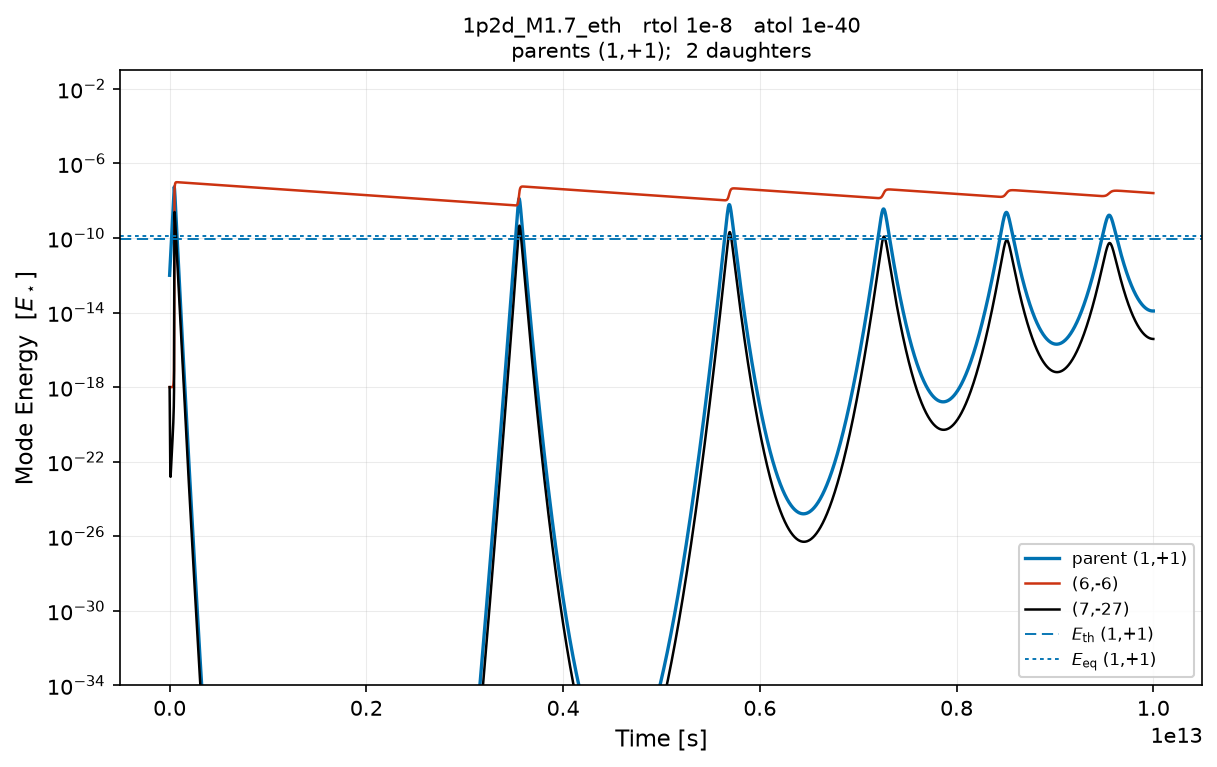
\includegraphics[width=0.21\textwidth,height=0.1323\textwidth]{../plots/rk8pd/1p2d_M1.7_eth/r1e-8_a1e-40.png} & 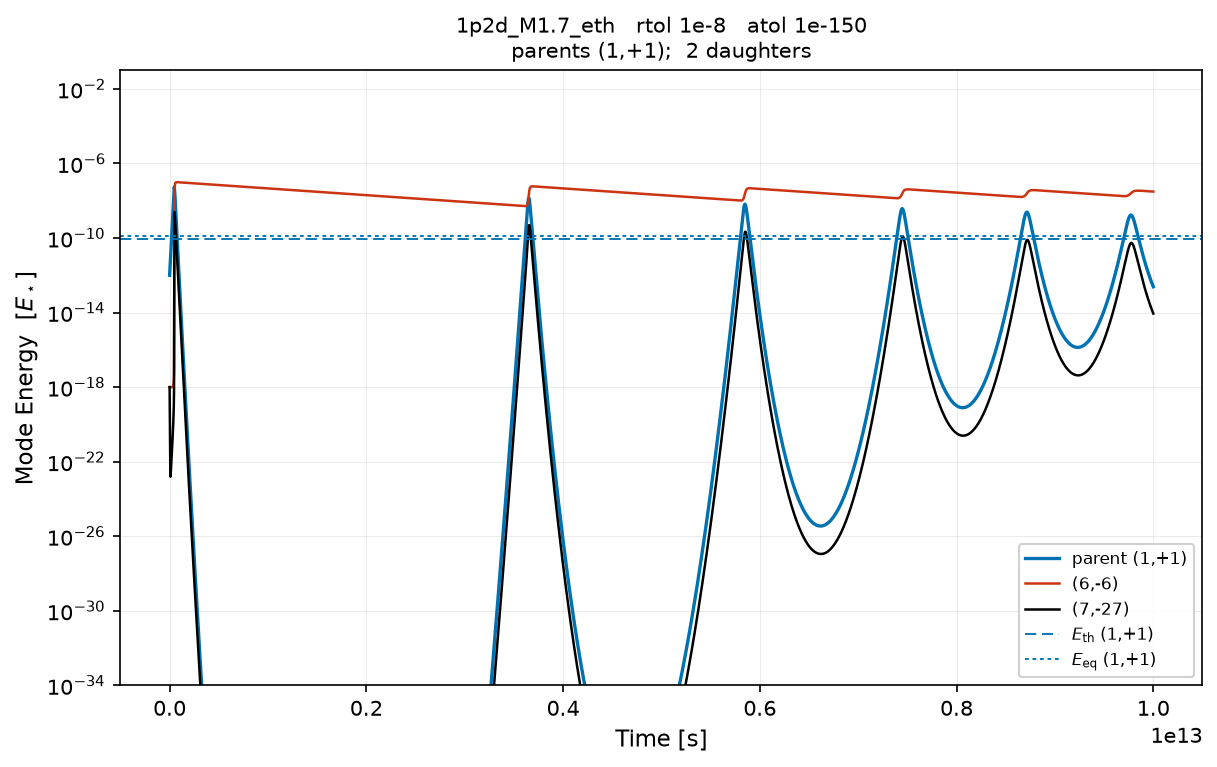
\includegraphics[width=0.21\textwidth,height=0.1323\textwidth]{../plots/rk8pd/1p2d_M1.7_eth/r1e-8_a1e-150.png} & 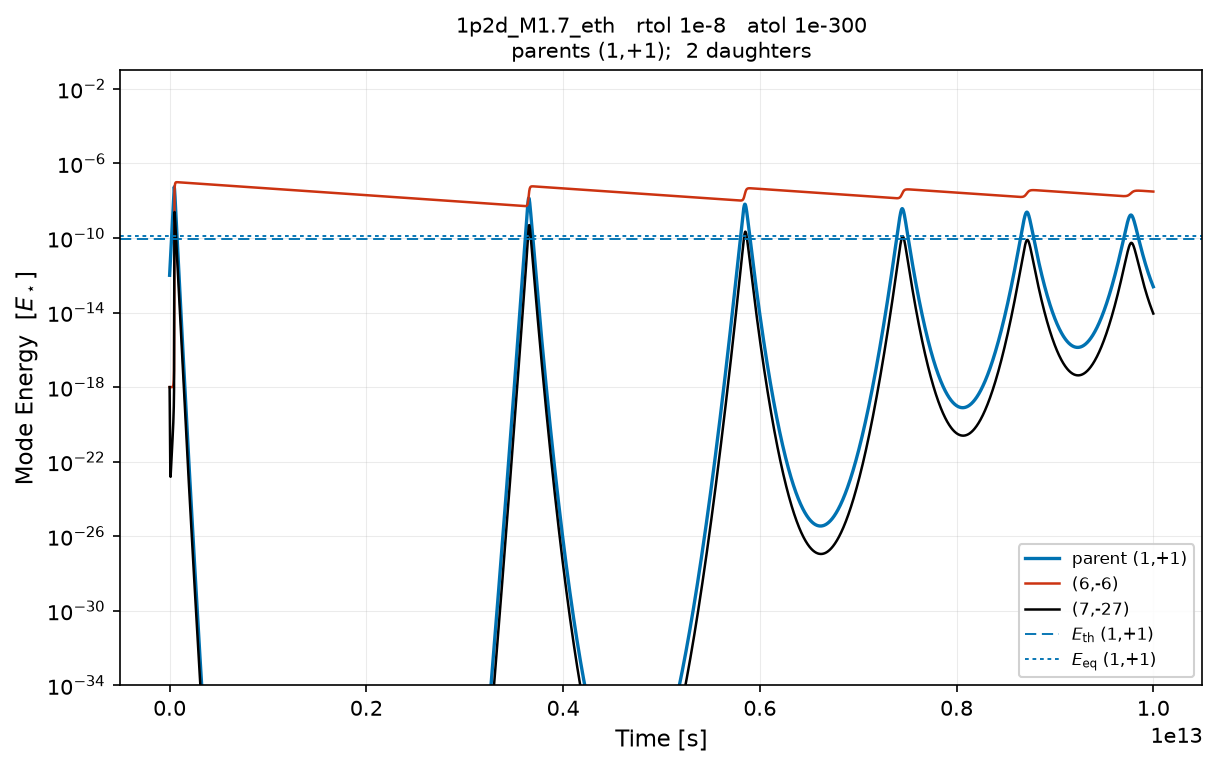
\includegraphics[width=0.21\textwidth,height=0.1323\textwidth]{../plots/rk8pd/1p2d_M1.7_eth/r1e-8_a1e-300.png} & 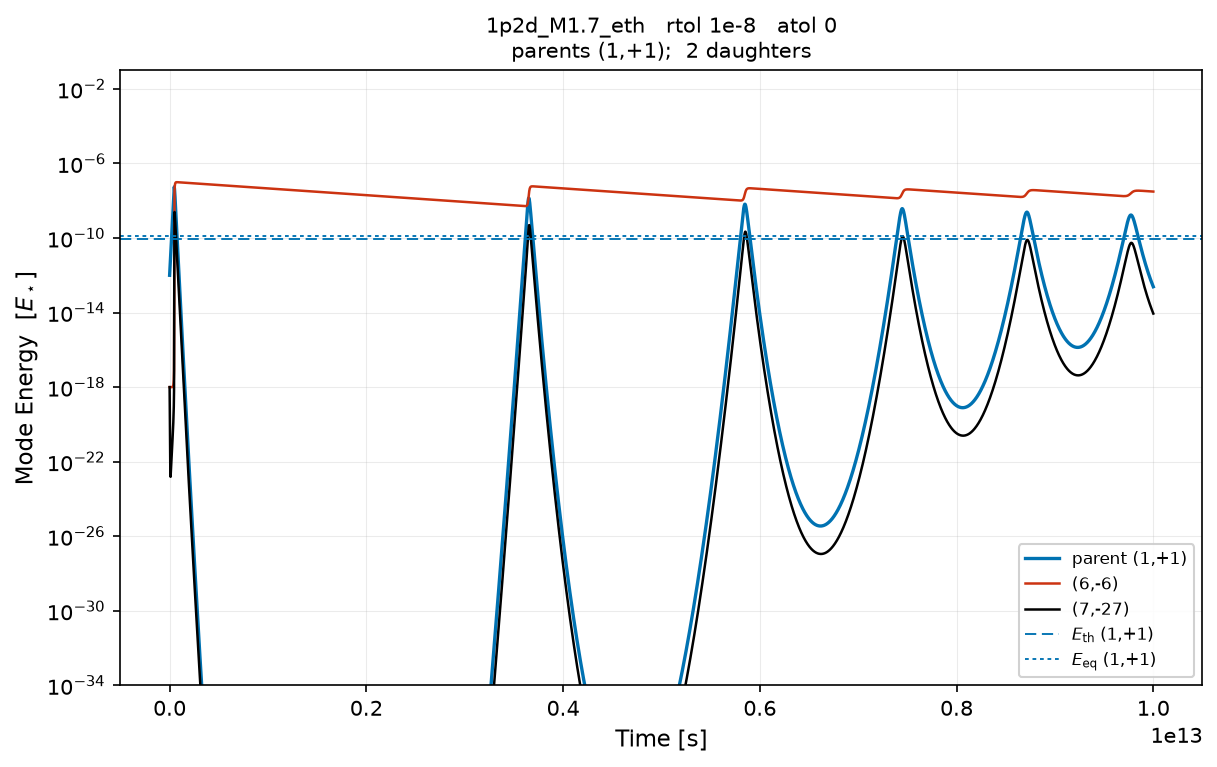
\includegraphics[width=0.21\textwidth,height=0.1323\textwidth]{../plots/rk8pd/1p2d_M1.7_eth/r1e-8_a0.png} \\[-1pt]
 & \parbox[t]{0.21\textwidth}{\centering\scriptsize 953.2\,k steps, 1.5\,s} & \parbox[t]{0.21\textwidth}{\centering\scriptsize 1.13\,M steps, 2.3\,s} & \parbox[t]{0.21\textwidth}{\centering\scriptsize 1.13\,M steps, 2.2\,s} & \parbox[t]{0.21\textwidth}{\centering\scriptsize 1.13\,M steps, 2.8\,s} \\[2pt]
\rotatebox{90}{\parbox{0.1323\textwidth}{\centering\scriptsize\bfseries BDF, dense analytic Jacobian}} & 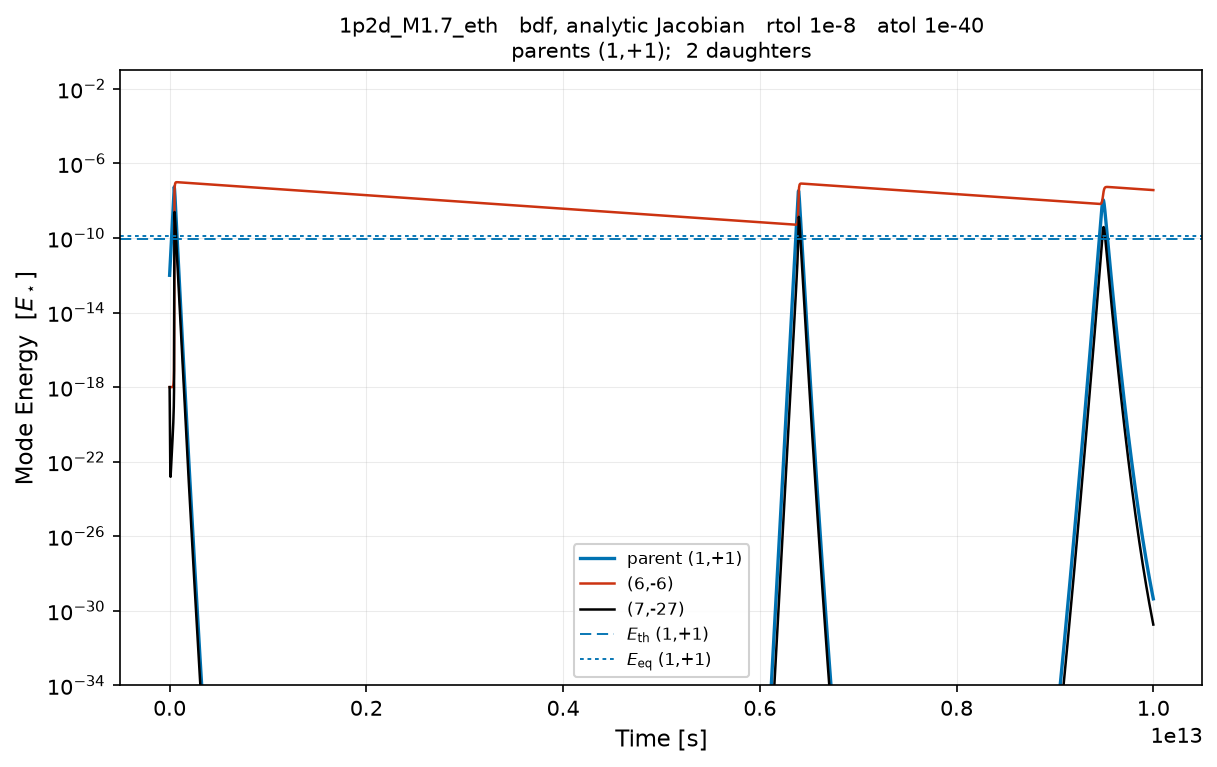
\includegraphics[width=0.21\textwidth,height=0.1323\textwidth]{../plots/bdf/1p2d_M1.7_eth/r1e-8_a1e-40.png} & 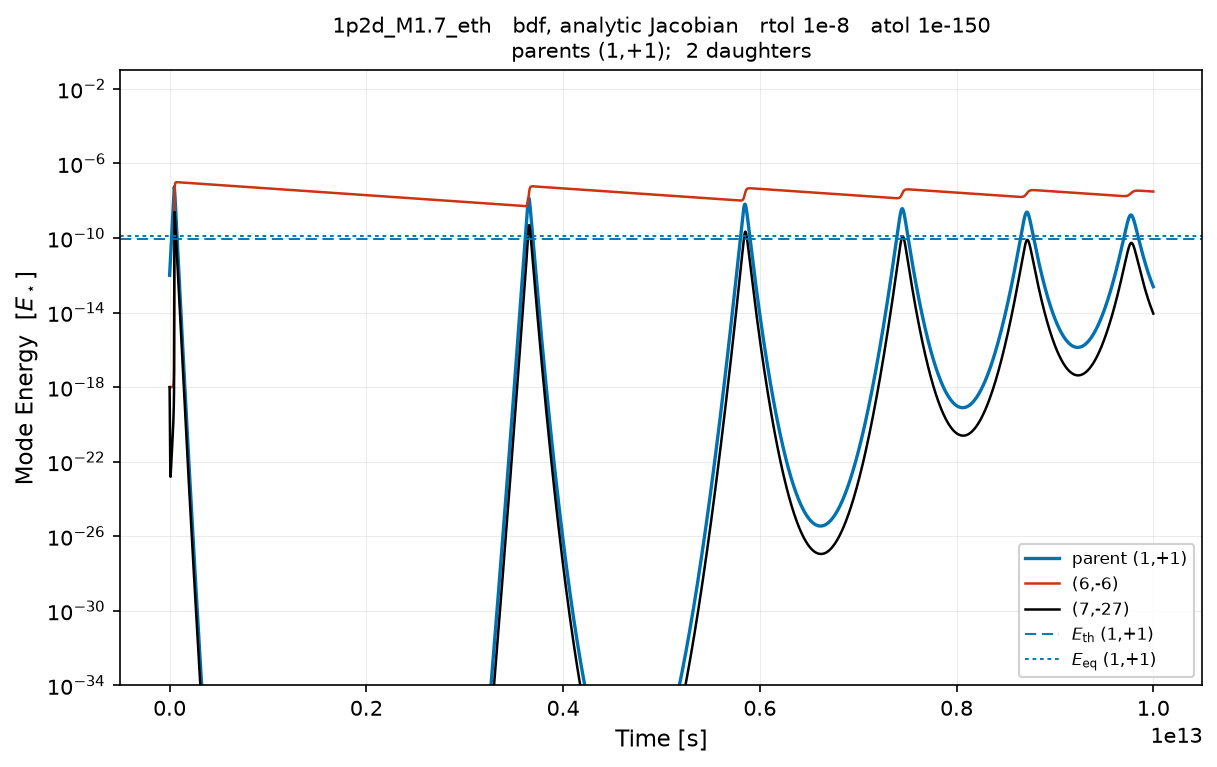
\includegraphics[width=0.21\textwidth,height=0.1323\textwidth]{../plots/bdf/1p2d_M1.7_eth/r1e-8_a1e-150.png} & 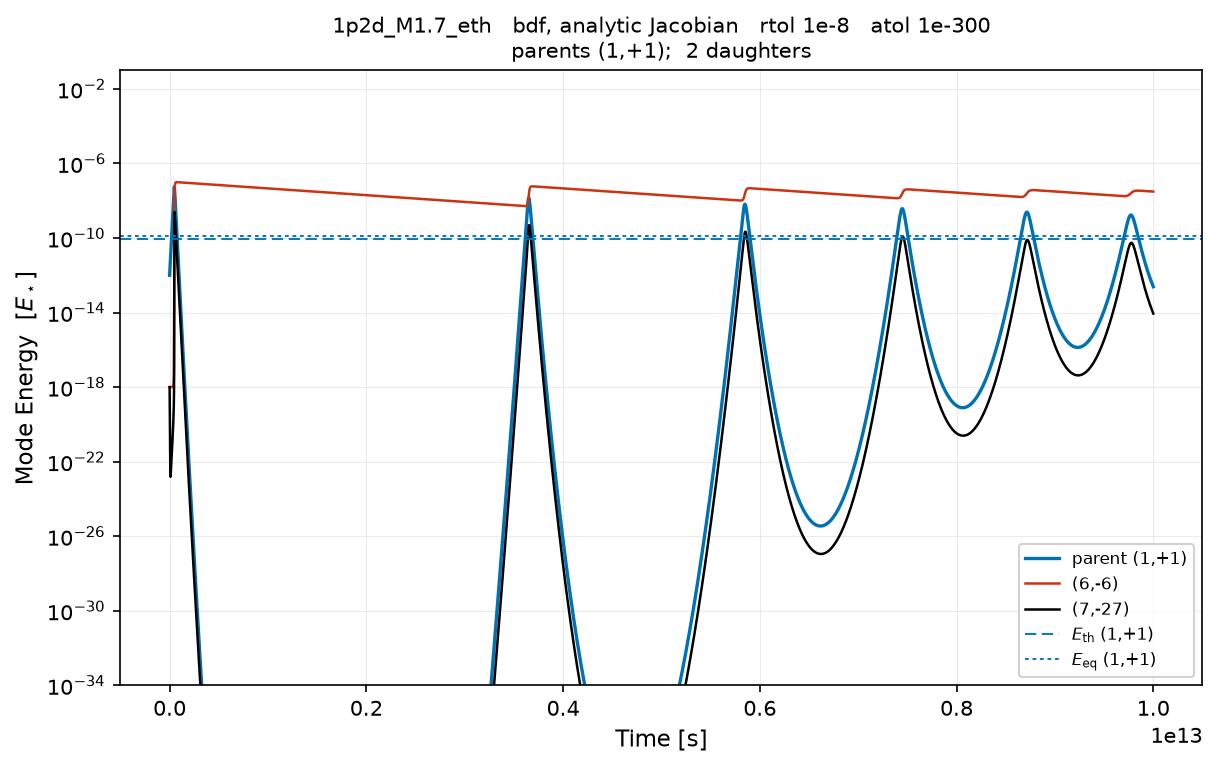
\includegraphics[width=0.21\textwidth,height=0.1323\textwidth]{../plots/bdf/1p2d_M1.7_eth/r1e-8_a1e-300.png} & 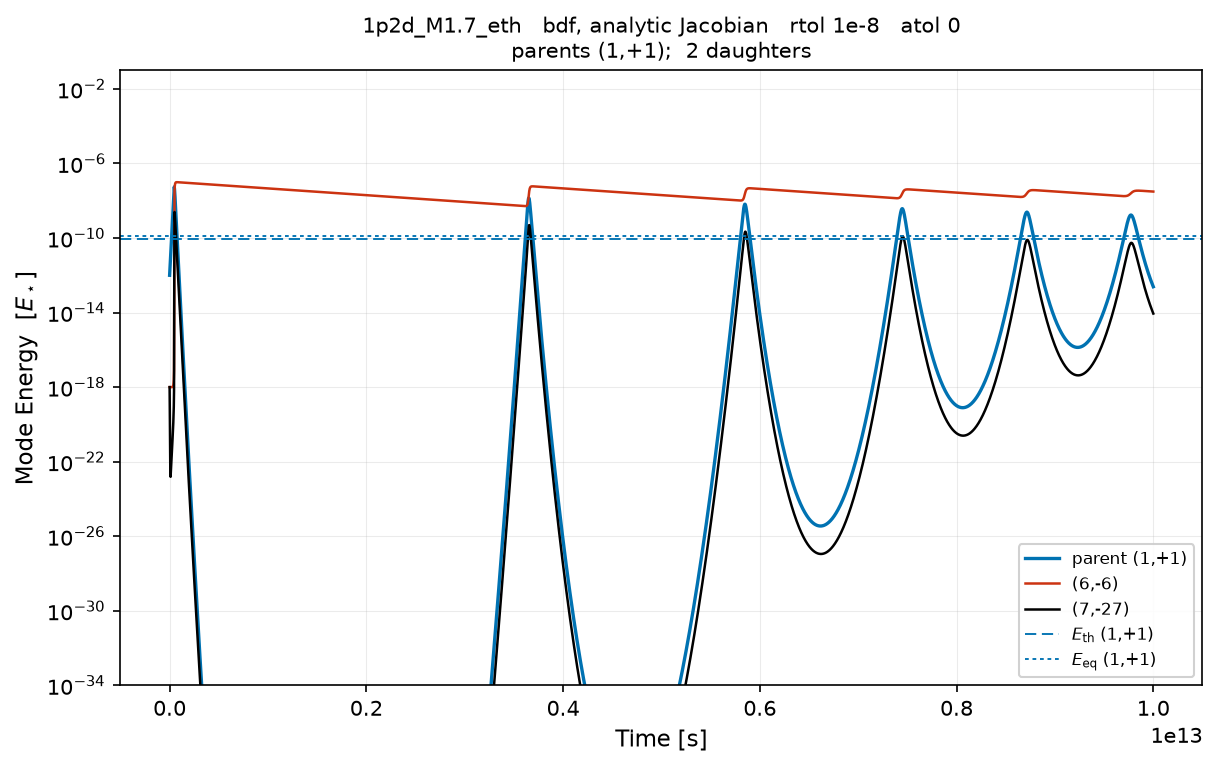
\includegraphics[width=0.21\textwidth,height=0.1323\textwidth]{../plots/bdf/1p2d_M1.7_eth/r1e-8_a0.png} \\[-1pt]
 & \parbox[t]{0.21\textwidth}{\centering\scriptsize 6.39\,M steps, 5.7\,s} & \parbox[t]{0.21\textwidth}{\centering\scriptsize 13.78\,M steps, 14.5\,s} & \parbox[t]{0.21\textwidth}{\centering\scriptsize 13.78\,M steps, 10.2\,s} & \parbox[t]{0.21\textwidth}{\centering\scriptsize 13.78\,M steps, 16.3\,s} \\[2pt]
\rotatebox{90}{\parbox{0.1323\textwidth}{\centering\scriptsize\bfseries BDF-Krylov, band full}} & 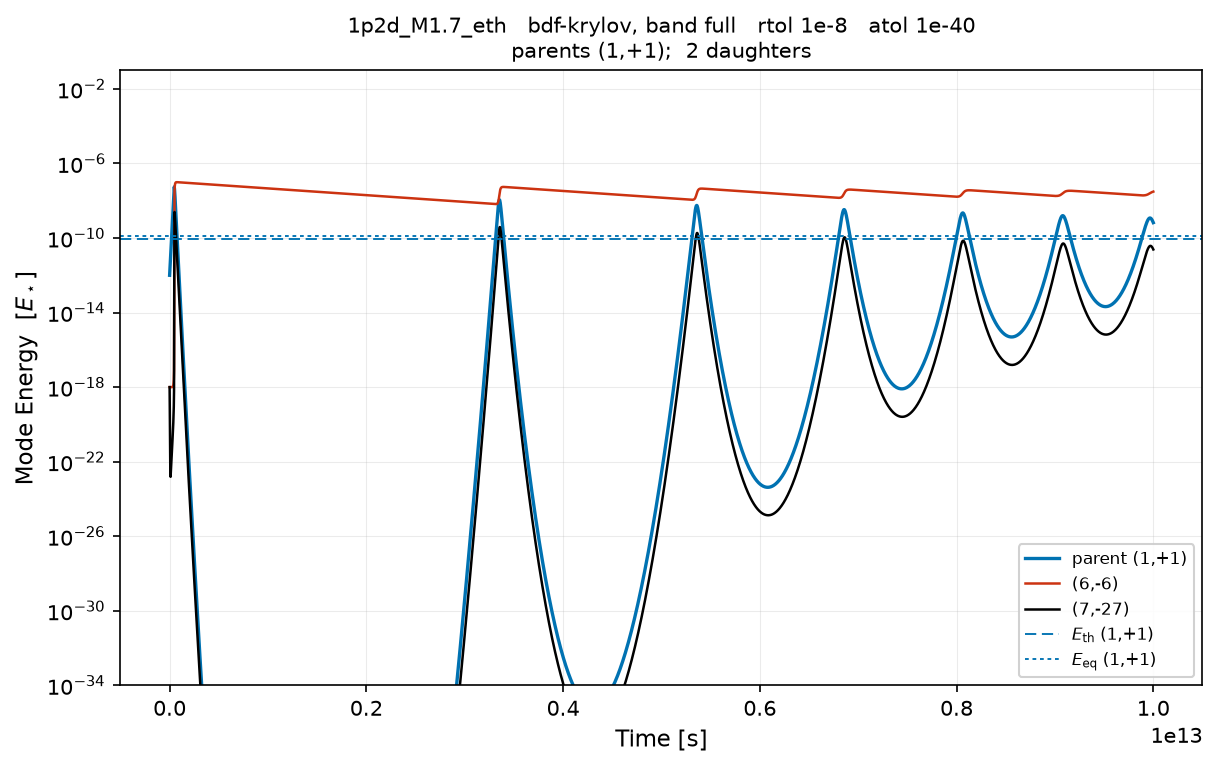
\includegraphics[width=0.21\textwidth,height=0.1323\textwidth]{../plots/krylov_full/1p2d_M1.7_eth/r1e-8_a1e-40.png} & 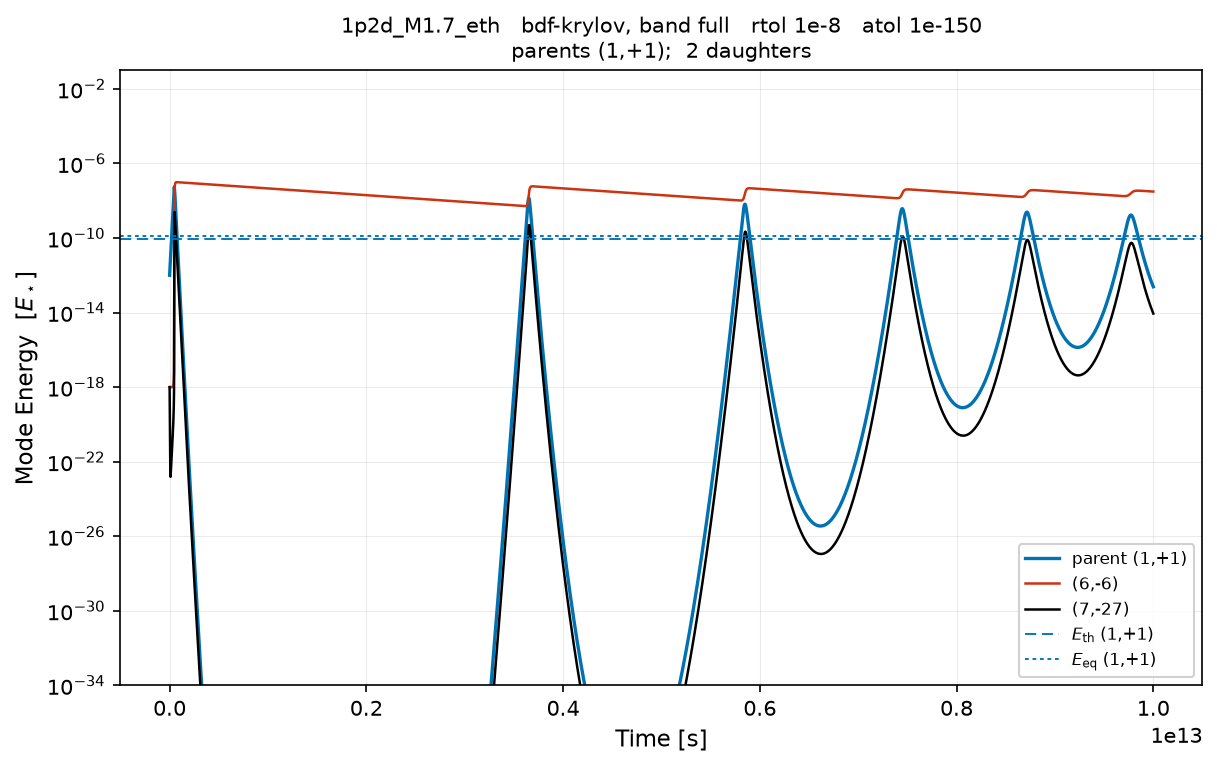
\includegraphics[width=0.21\textwidth,height=0.1323\textwidth]{../plots/krylov_full/1p2d_M1.7_eth/r1e-8_a1e-150.png} & 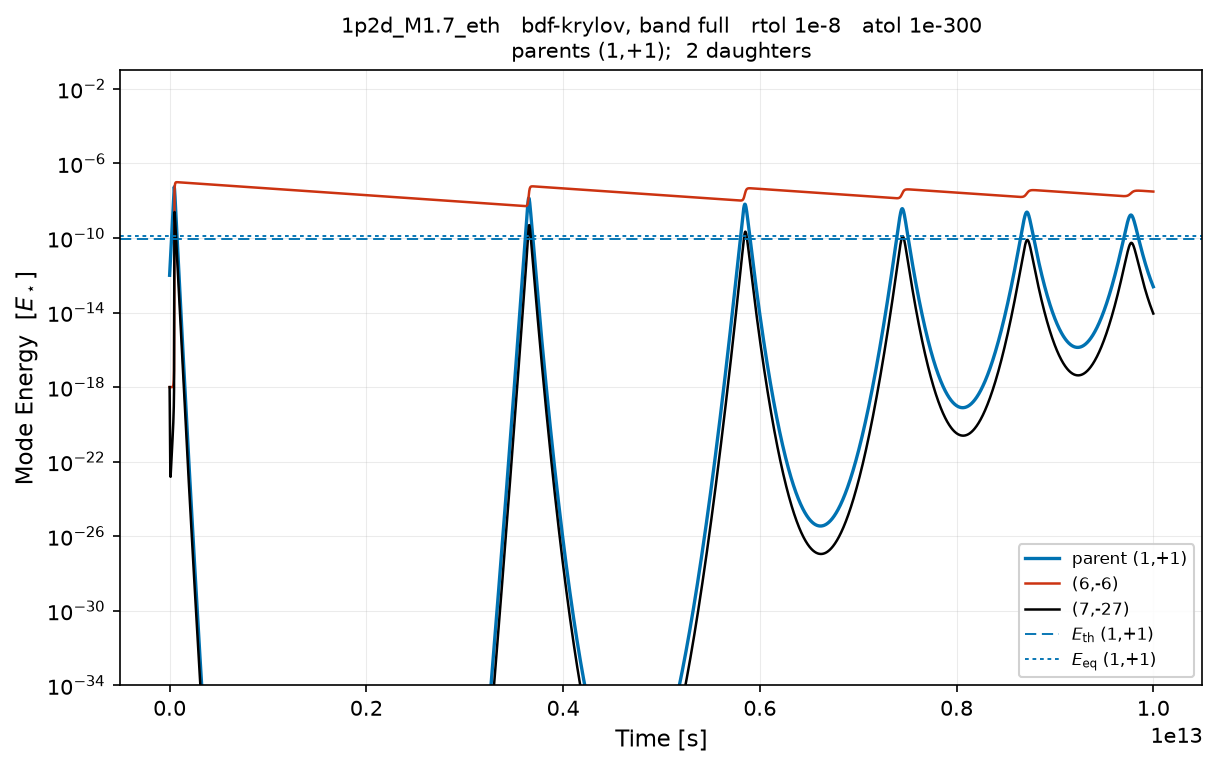
\includegraphics[width=0.21\textwidth,height=0.1323\textwidth]{../plots/krylov_full/1p2d_M1.7_eth/r1e-8_a1e-300.png} & 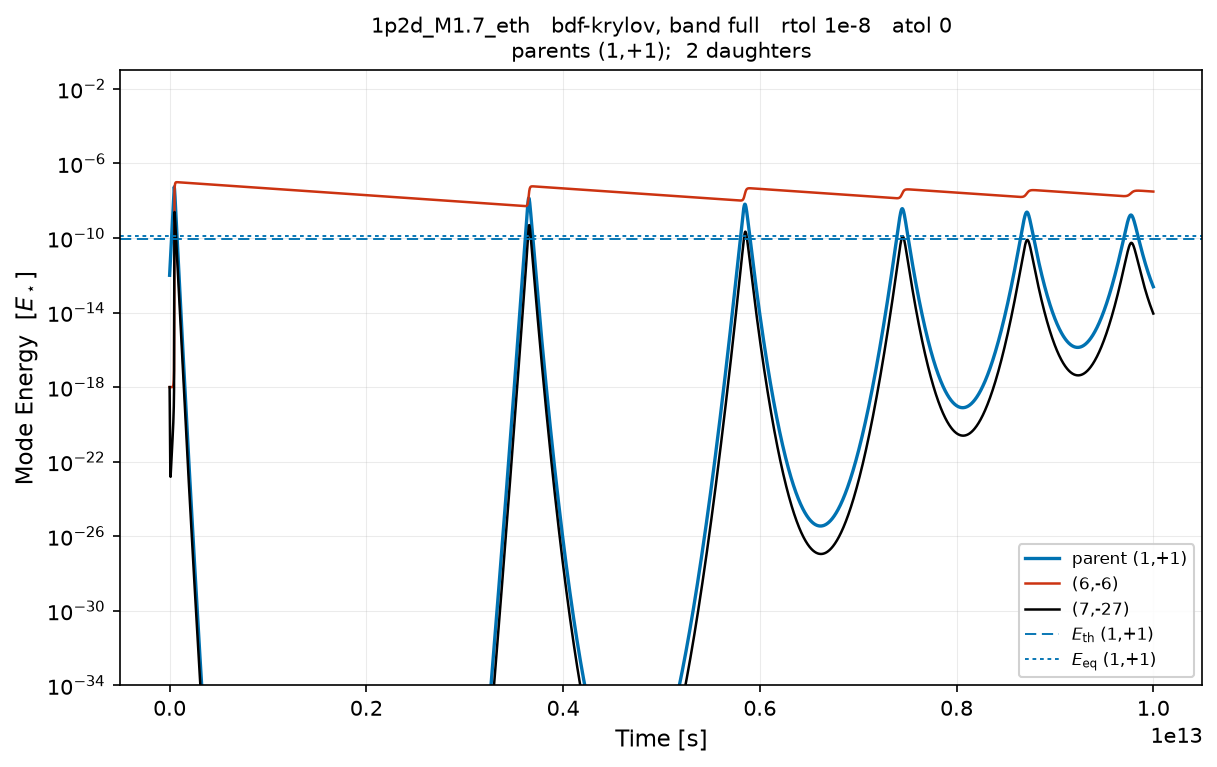
\includegraphics[width=0.21\textwidth,height=0.1323\textwidth]{../plots/krylov_full/1p2d_M1.7_eth/r1e-8_a0.png} \\[-1pt]
 & \parbox[t]{0.21\textwidth}{\centering\scriptsize 12.00\,M steps, 22.8\,s} & \parbox[t]{0.21\textwidth}{\centering\scriptsize 13.44\,M steps, 25.5\,s} & \parbox[t]{0.21\textwidth}{\centering\scriptsize 13.44\,M steps, 17.4\,s} & \parbox[t]{0.21\textwidth}{\centering\scriptsize 13.44\,M steps, 16.8\,s} \\[2pt]
\rotatebox{90}{\parbox{0.1323\textwidth}{\centering\scriptsize\bfseries BDF-Krylov, band 3}} & 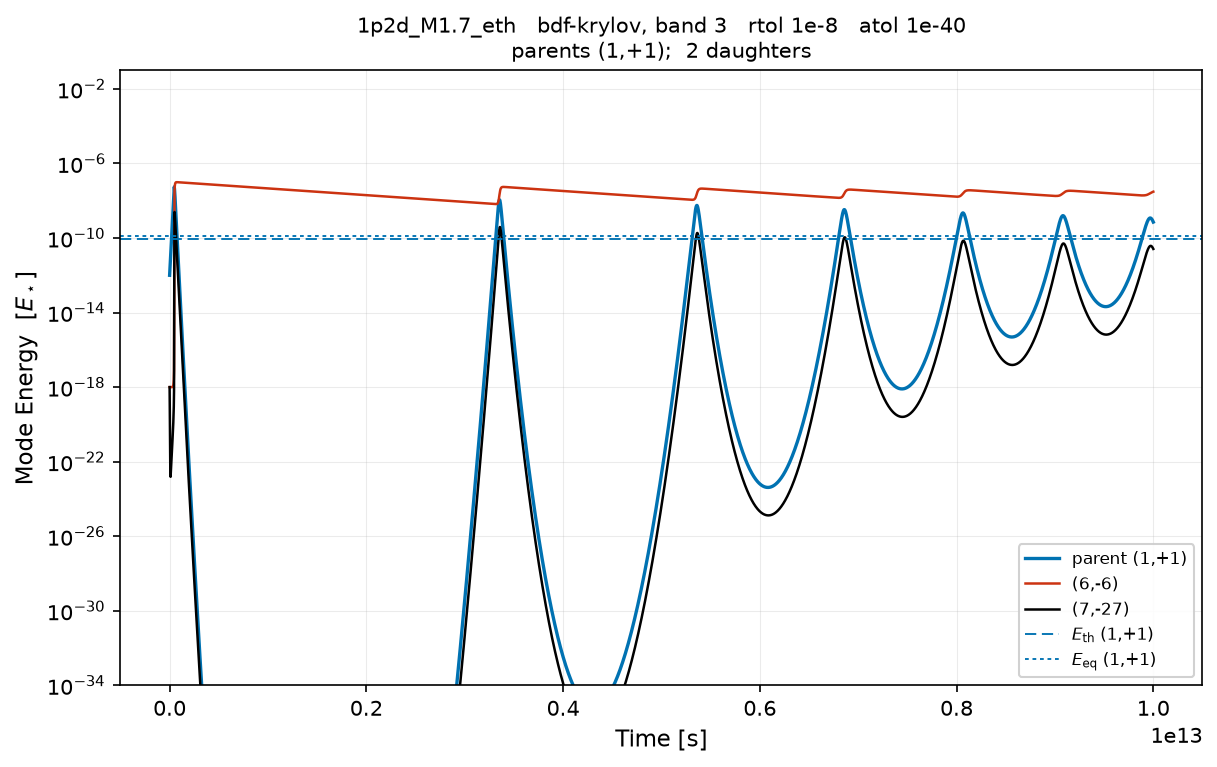
\includegraphics[width=0.21\textwidth,height=0.1323\textwidth]{../plots/krylov_b3/1p2d_M1.7_eth/r1e-8_a1e-40.png} & 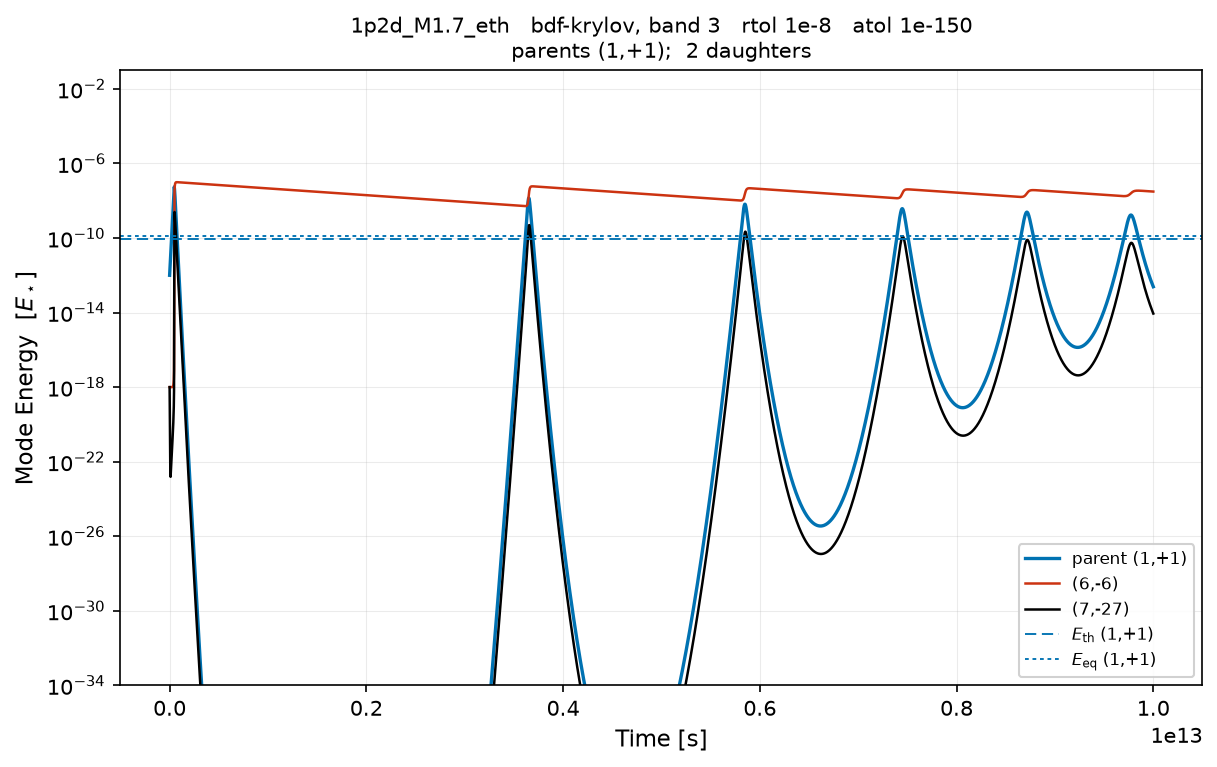
\includegraphics[width=0.21\textwidth,height=0.1323\textwidth]{../plots/krylov_b3/1p2d_M1.7_eth/r1e-8_a1e-150.png} & 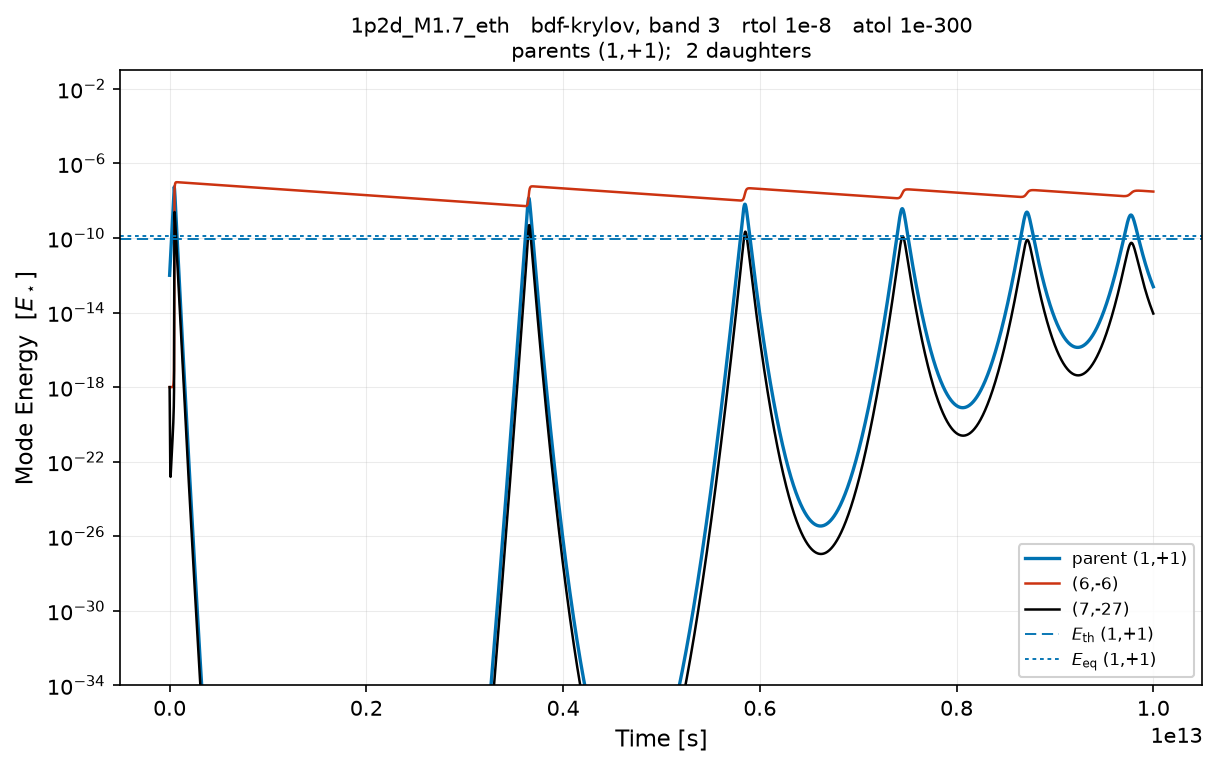
\includegraphics[width=0.21\textwidth,height=0.1323\textwidth]{../plots/krylov_b3/1p2d_M1.7_eth/r1e-8_a1e-300.png} & 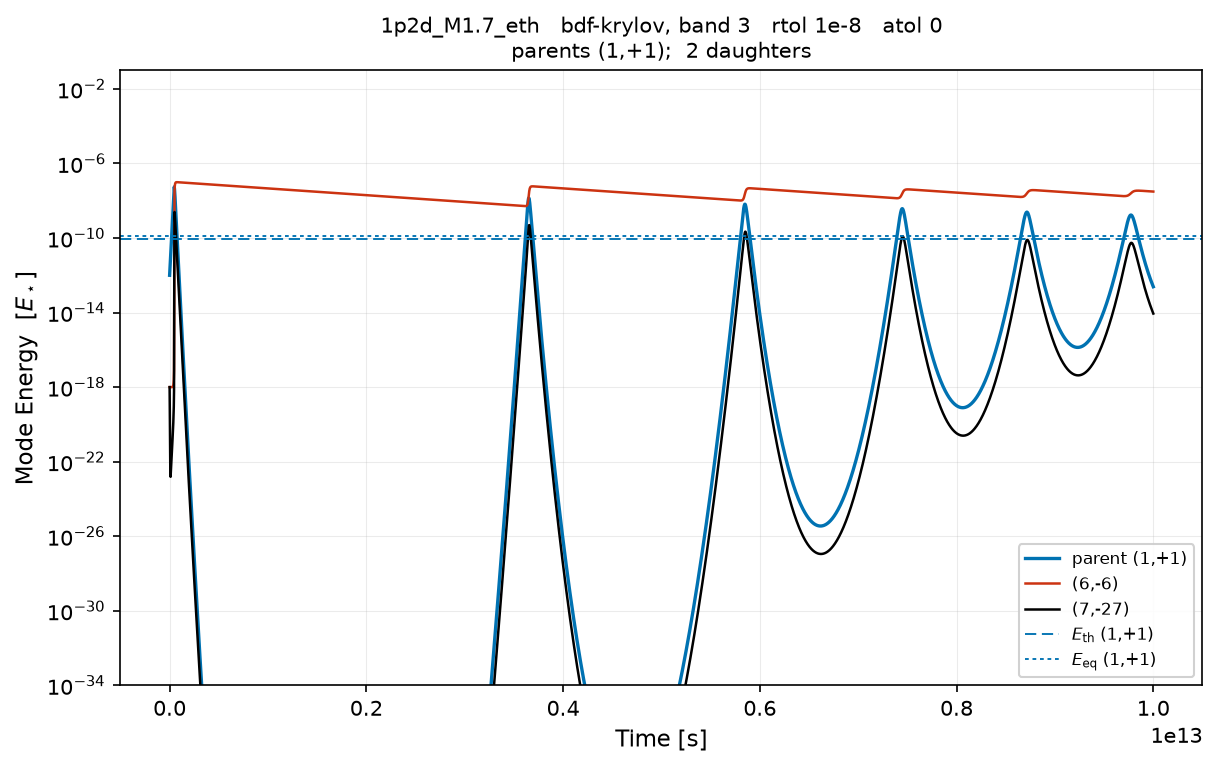
\includegraphics[width=0.21\textwidth,height=0.1323\textwidth]{../plots/krylov_b3/1p2d_M1.7_eth/r1e-8_a0.png} \\[-1pt]
 & \parbox[t]{0.21\textwidth}{\centering\scriptsize 11.86\,M steps, 16.6\,s} & \parbox[t]{0.21\textwidth}{\centering\scriptsize 13.28\,M steps, 20.7\,s} & \parbox[t]{0.21\textwidth}{\centering\scriptsize 13.28\,M steps, 25.0\,s} & \parbox[t]{0.21\textwidth}{\centering\scriptsize 13.28\,M steps, 14.9\,s} \\[2pt]
\rotatebox{90}{\parbox{0.1323\textwidth}{\centering\scriptsize\bfseries Adams, fixed point}} & 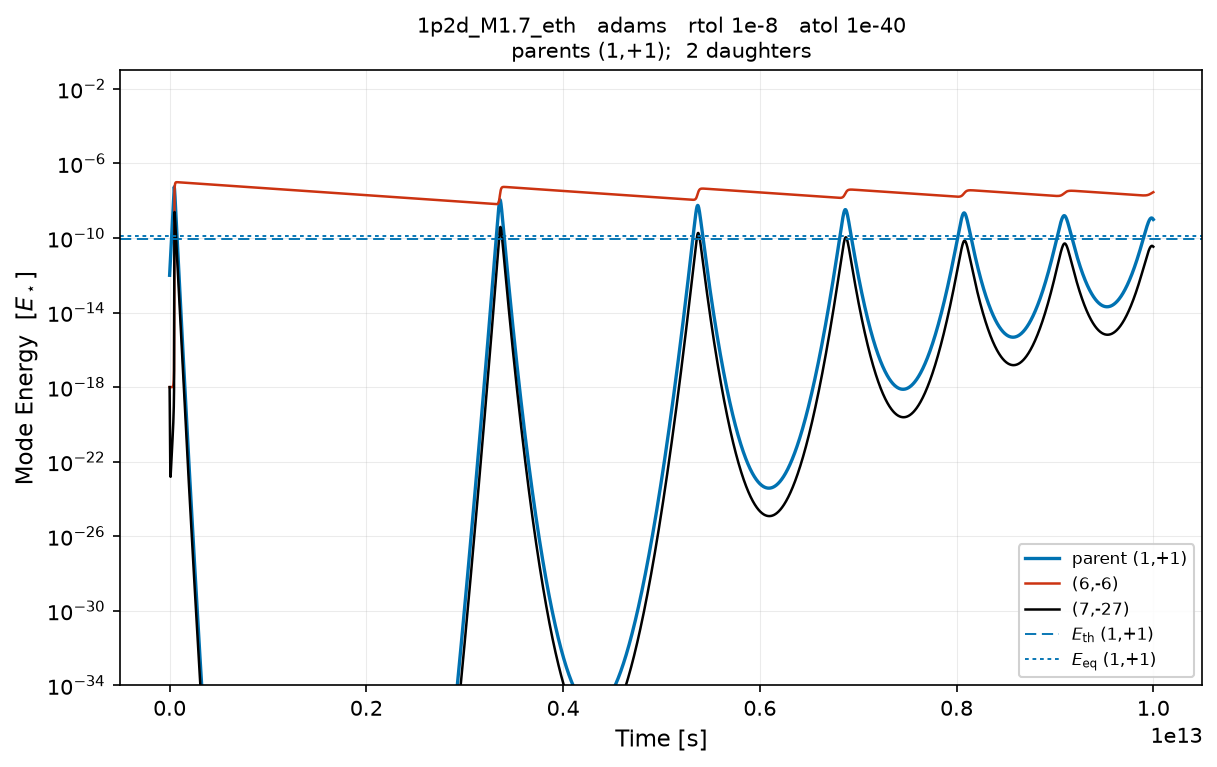
\includegraphics[width=0.21\textwidth,height=0.1323\textwidth]{../plots/adams/1p2d_M1.7_eth/r1e-8_a1e-40.png} & 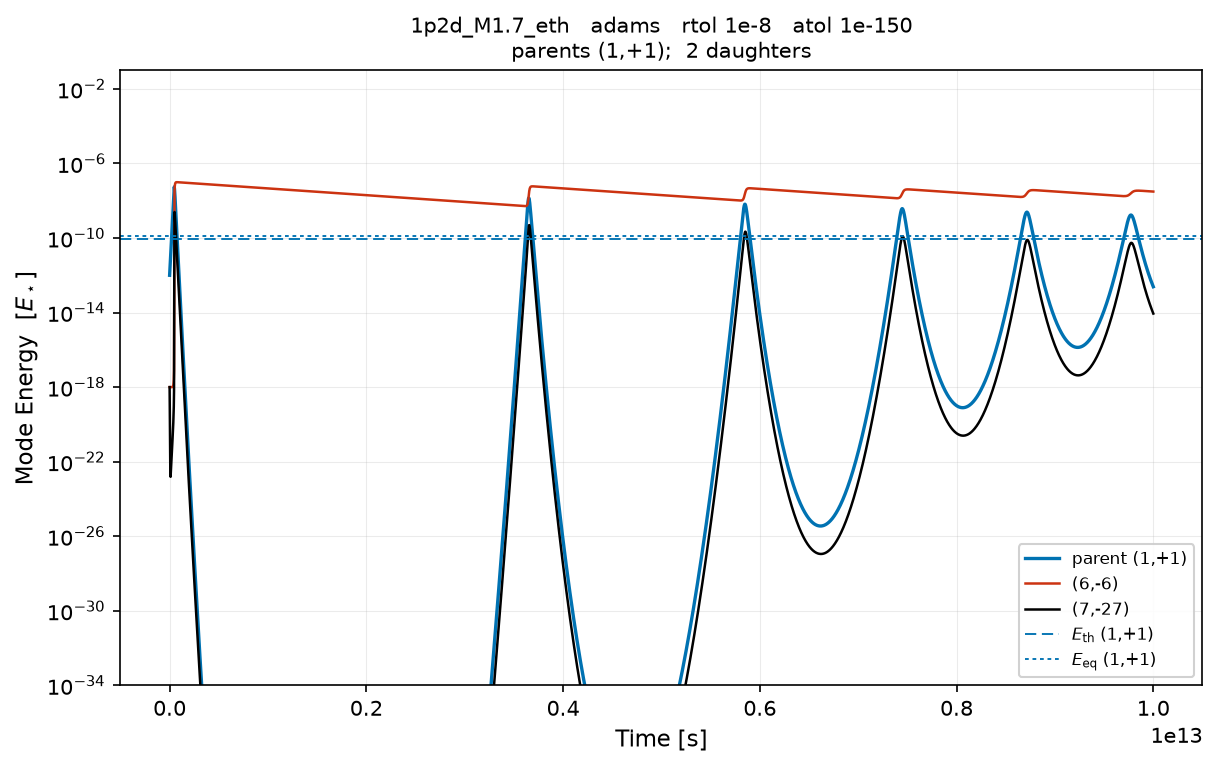
\includegraphics[width=0.21\textwidth,height=0.1323\textwidth]{../plots/adams/1p2d_M1.7_eth/r1e-8_a1e-150.png} & 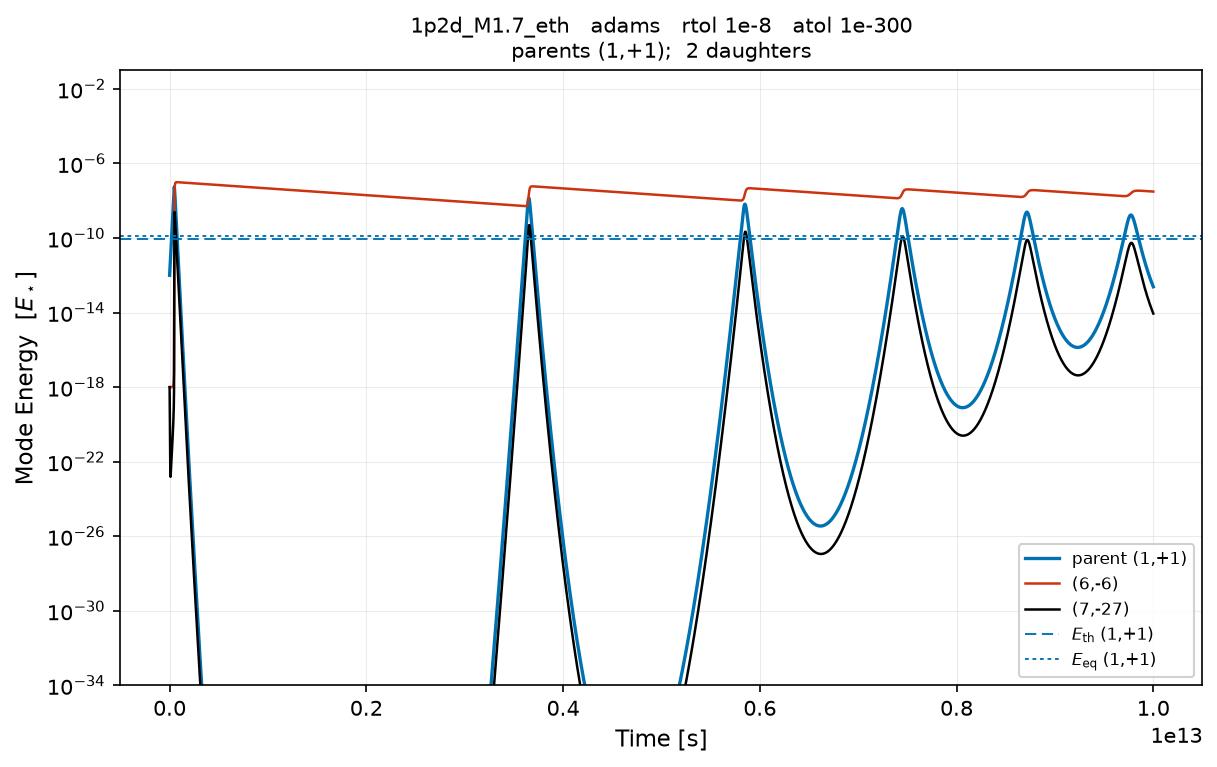
\includegraphics[width=0.21\textwidth,height=0.1323\textwidth]{../plots/adams/1p2d_M1.7_eth/r1e-8_a1e-300.png} & 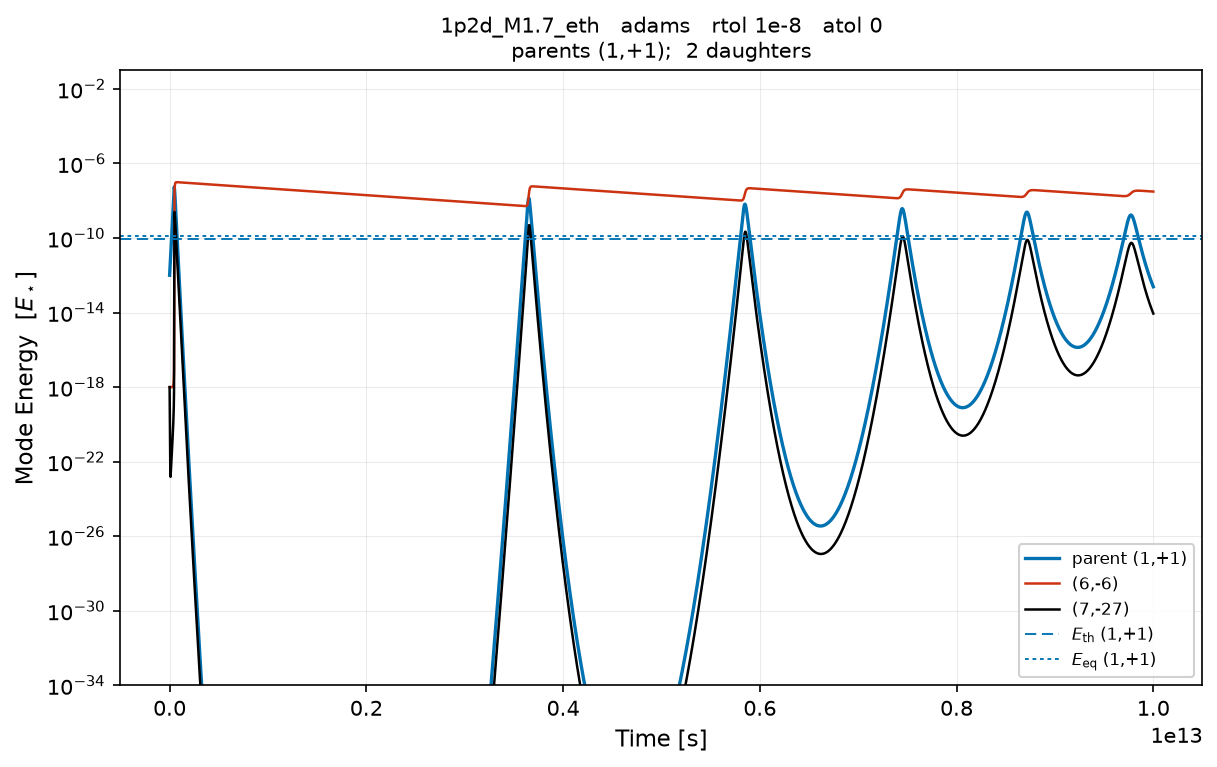
\includegraphics[width=0.21\textwidth,height=0.1323\textwidth]{../plots/adams/1p2d_M1.7_eth/r1e-8_a0.png} \\[-1pt]
 & \parbox[t]{0.21\textwidth}{\centering\scriptsize 5.47\,M steps, 7.2\,s} & \parbox[t]{0.21\textwidth}{\centering\scriptsize 5.88\,M steps, 8.0\,s} & \parbox[t]{0.21\textwidth}{\centering\scriptsize 5.88\,M steps, 8.0\,s} & \parbox[t]{0.21\textwidth}{\centering\scriptsize 5.88\,M steps, 8.0\,s} \\[2pt]
\end{tabular}\par}
\par\noindent{\scriptsize\setlength\tabcolsep{3.5pt}\renewcommand\arraystretch{0.92}
\begin{tabular}{@{}llllrrrrrrr@{}}
\toprule
integrator & atol & stop & $t_{\rm stop}$ [s] & steps & rejected & RHS & Jac. & NL it. & lin. it. & wall [s] \\
\midrule
rk8pd & $10^{-40}$ & end & $1.00\times10^{13}$ & 953.2\,k & 101.3\,k & 12.39\,M & -- & -- & -- & 1.5 \\
 & $10^{-150}$ & end & $1.00\times10^{13}$ & 1.13\,M & 126.8\,k & 14.65\,M & -- & -- & -- & 2.3 \\
 & $10^{-300}$ & end & $1.00\times10^{13}$ & 1.13\,M & 126.8\,k & 14.65\,M & -- & -- & -- & 2.2 \\
 & $0$ & end & $1.00\times10^{13}$ & 1.13\,M & 126.8\,k & 14.65\,M & -- & -- & -- & 2.8 \\
\addlinespace[2pt]
BDF, dense analytic Jacobian & $10^{-40}$ & end & $1.00\times10^{13}$ & 6.39\,M & 49.0\,k & 6.85\,M & 117.8\,k & 6.85\,M & -- & 5.7 \\
 & $10^{-150}$ & end & $1.00\times10^{13}$ & 13.78\,M & 118.0\,k & 14.74\,M & 241.1\,k & 14.74\,M & -- & 14.5 \\
 & $10^{-300}$ & end & $1.00\times10^{13}$ & 13.78\,M & 118.0\,k & 14.74\,M & 241.1\,k & 14.74\,M & -- & 10.2 \\
 & $0$ & end & $1.00\times10^{13}$ & 13.78\,M & 118.0\,k & 14.74\,M & 241.1\,k & 14.74\,M & -- & 16.3 \\
\addlinespace[2pt]
BDF-Krylov, band full & $10^{-40}$ & end & $1.00\times10^{13}$ & 12.00\,M & 104.9\,k & 27.04\,M & 209.5\,k & 12.90\,M & 12.88\,M & 22.8 \\
 & $10^{-150}$ & end & $1.00\times10^{13}$ & 13.44\,M & 125.8\,k & 29.86\,M & 234.6\,k & 14.47\,M & 13.98\,M & 25.5 \\
 & $10^{-300}$ & end & $1.00\times10^{13}$ & 13.44\,M & 125.8\,k & 29.86\,M & 234.6\,k & 14.47\,M & 13.98\,M & 17.4 \\
 & $0$ & end & $1.00\times10^{13}$ & 13.44\,M & 125.8\,k & 29.86\,M & 234.6\,k & 14.47\,M & 13.98\,M & 16.8 \\
\addlinespace[2pt]
BDF-Krylov, band 3 & $10^{-40}$ & end & $1.00\times10^{13}$ & 11.86\,M & 110.2\,k & 26.98\,M & 207.1\,k & 12.80\,M & 12.94\,M & 16.6 \\
 & $10^{-150}$ & end & $1.00\times10^{13}$ & 13.28\,M & 132.1\,k & 29.80\,M & 231.8\,k & 14.35\,M & 14.05\,M & 20.7 \\
 & $10^{-300}$ & end & $1.00\times10^{13}$ & 13.28\,M & 132.1\,k & 29.80\,M & 231.8\,k & 14.35\,M & 14.05\,M & 25.0 \\
 & $0$ & end & $1.00\times10^{13}$ & 13.28\,M & 132.1\,k & 29.80\,M & 231.8\,k & 14.35\,M & 14.05\,M & 14.9 \\
\addlinespace[2pt]
Adams, fixed point & $10^{-40}$ & end & $1.00\times10^{13}$ & 5.47\,M & 231.7\,k & 8.22\,M & -- & 8.22\,M & -- & 7.2 \\
 & $10^{-150}$ & end & $1.00\times10^{13}$ & 5.88\,M & 285.4\,k & 8.57\,M & -- & 8.57\,M & -- & 8.0 \\
 & $10^{-300}$ & end & $1.00\times10^{13}$ & 5.88\,M & 285.4\,k & 8.57\,M & -- & 8.57\,M & -- & 8.0 \\
 & $0$ & end & $1.00\times10^{13}$ & 5.88\,M & 285.4\,k & 8.57\,M & -- & 8.57\,M & -- & 8.0 \\
\bottomrule
\end{tabular}}

\clearpage
\subsection{\texttt{1p2d\_M2.0T\_eth}}\label{net:1p2d_M2.0T_eth}
\noindent\begin{minipage}[t]{0.43\textwidth}\vspace{0pt}\footnotesize
\begin{tabular}{@{}rrlrr@{}}
\toprule
id & gen & $(\ell,n)$ & $\omega$ [rad\,s$^{-1}$] & $\gamma$ [s$^{-1}$] \\
\midrule
0 & 0 & (2,$-$2) & $7.959\times10^{-4}$ & $-6.697\times10^{-11}$ \\
1 & 1 & (3,$-$31) & $1.287\times10^{-4}$ & $8.096\times10^{-11}$ \\
2 & 1 & (5,$-$8) & $6.672\times10^{-4}$ & $7.367\times10^{-13}$ \\
\bottomrule
\end{tabular}
\end{minipage}\hfill
\begin{minipage}[t]{0.55\textwidth}\vspace{0pt}\footnotesize
\textbf{Model} \texttt{dsct\_M2.0\_T7696}, rule eth, $N=1$, cut 0.15,
closure 0.005; 3 modes, 1 triplet(s).\\[2pt]
\textbf{Selecting pairs}\\ (2,$-$2) $\to$ (3,$-$31) + (5,$-$8): $\Delta/\omega_a=-3.69\times10^{-6}$, $\kappa=+0.215$, $E_{\rm th}=4.87\times10^{-12}$, $E_{\rm eq}=1.50\times10^{-10}$\\[2pt]

\end{minipage}

\par\smallskip{\centering\begin{tabular}{@{}c@{\hspace{2pt}}c@{\hspace{2pt}}c@{\hspace{2pt}}c@{\hspace{2pt}}c@{}}
 & \small atol $10^{-40}$ & \small atol $10^{-150}$ & \small atol $10^{-300}$ & \small atol $0$ \\[1pt]
\rotatebox{90}{\parbox{0.1323\textwidth}{\centering\scriptsize\bfseries rk8pd}} & 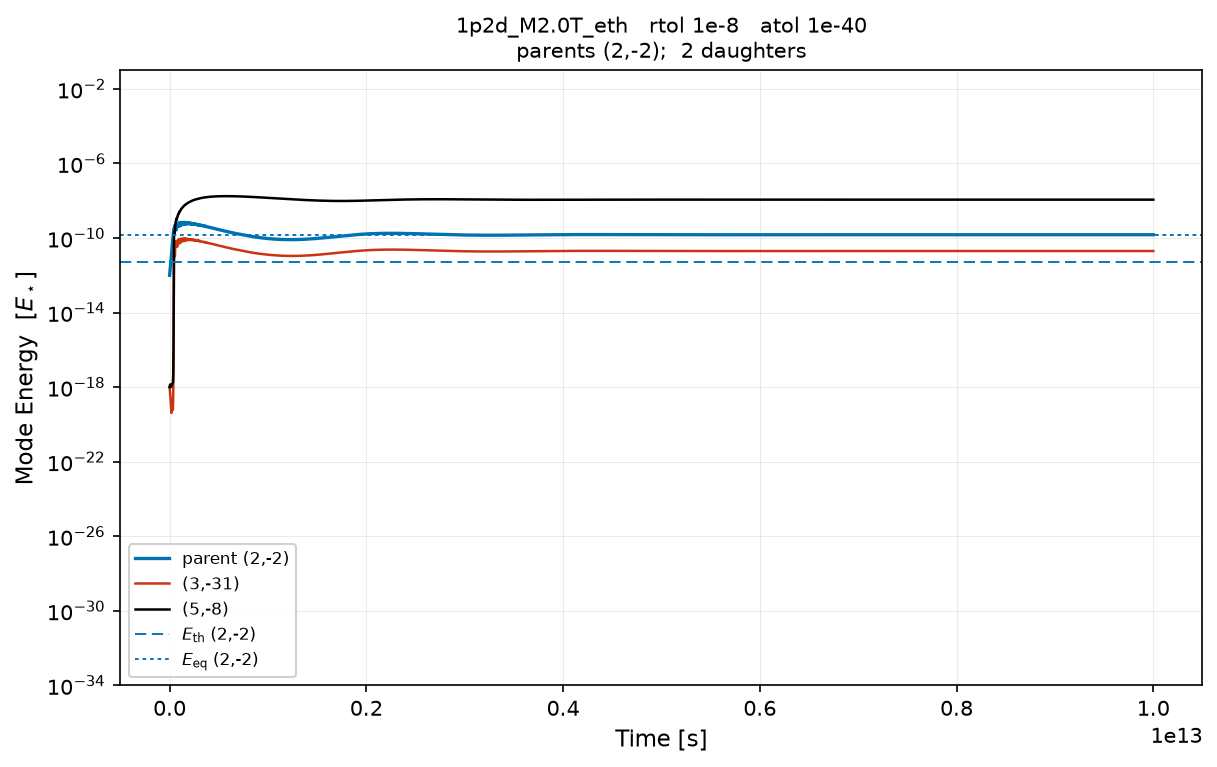
\includegraphics[width=0.21\textwidth,height=0.1323\textwidth]{../plots/rk8pd/1p2d_M2.0T_eth/r1e-8_a1e-40.png} & 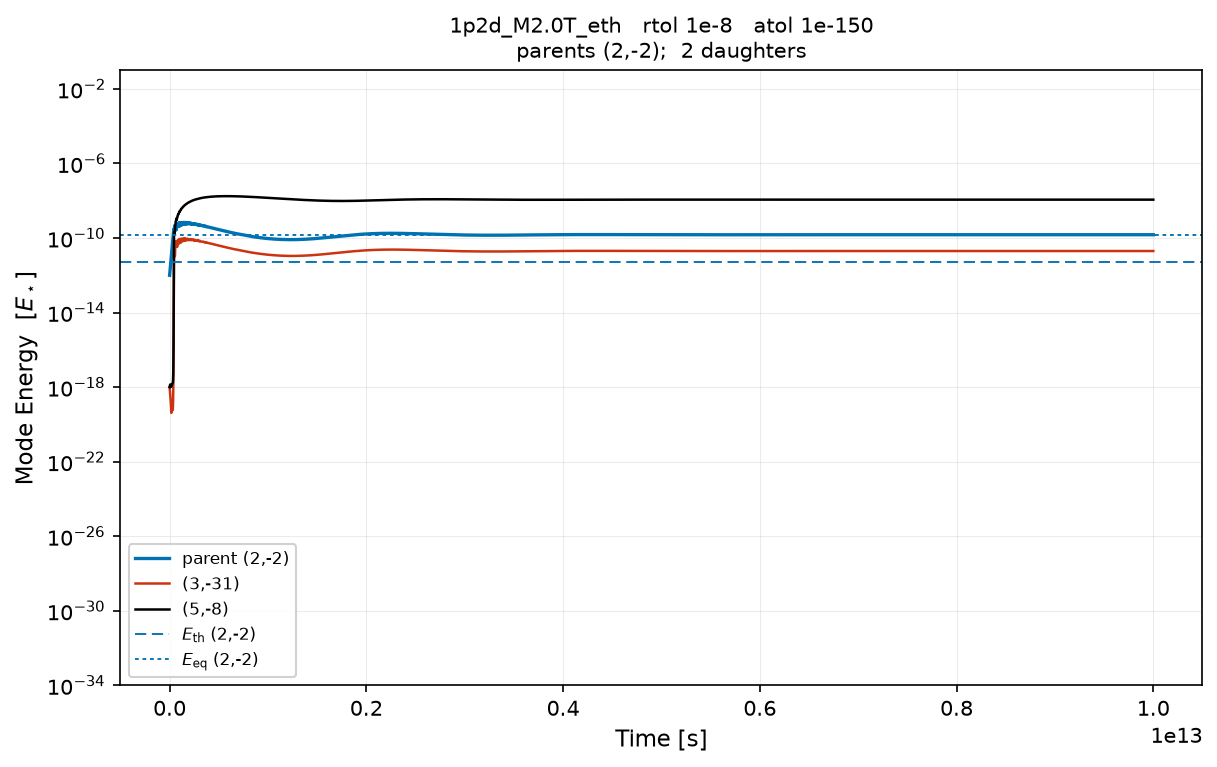
\includegraphics[width=0.21\textwidth,height=0.1323\textwidth]{../plots/rk8pd/1p2d_M2.0T_eth/r1e-8_a1e-150.png} & 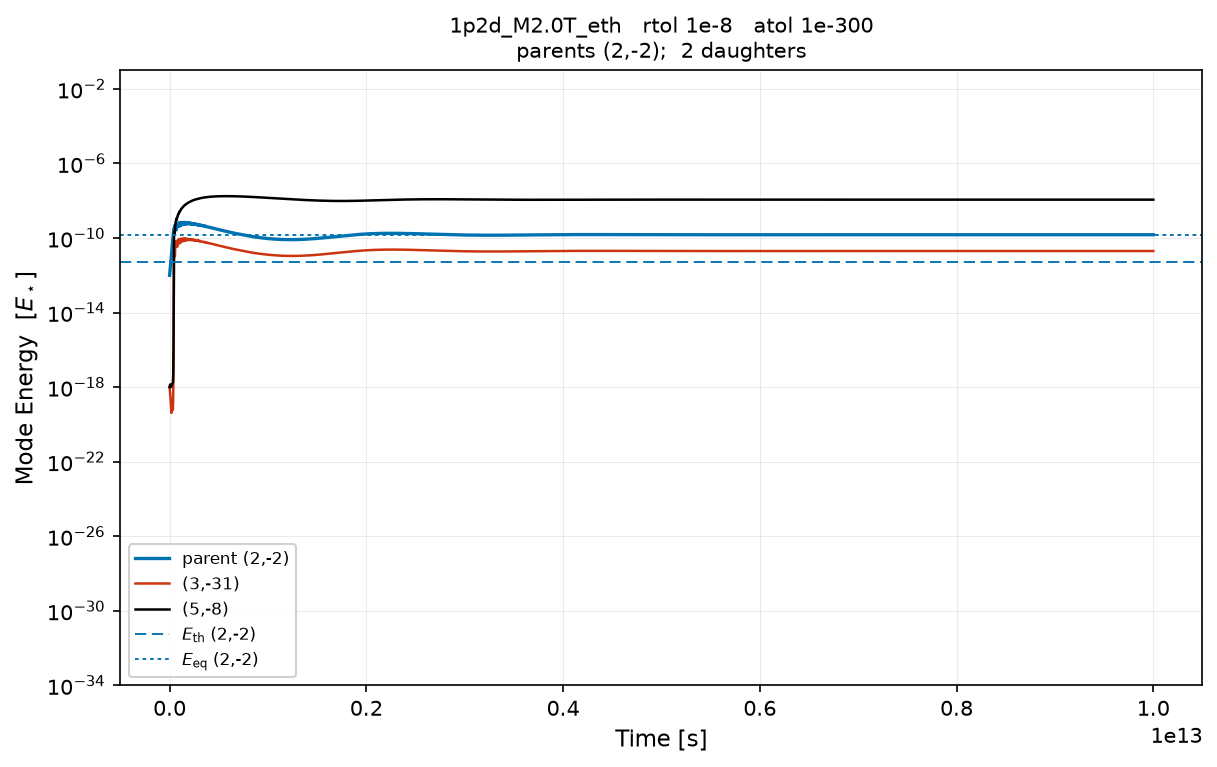
\includegraphics[width=0.21\textwidth,height=0.1323\textwidth]{../plots/rk8pd/1p2d_M2.0T_eth/r1e-8_a1e-300.png} & 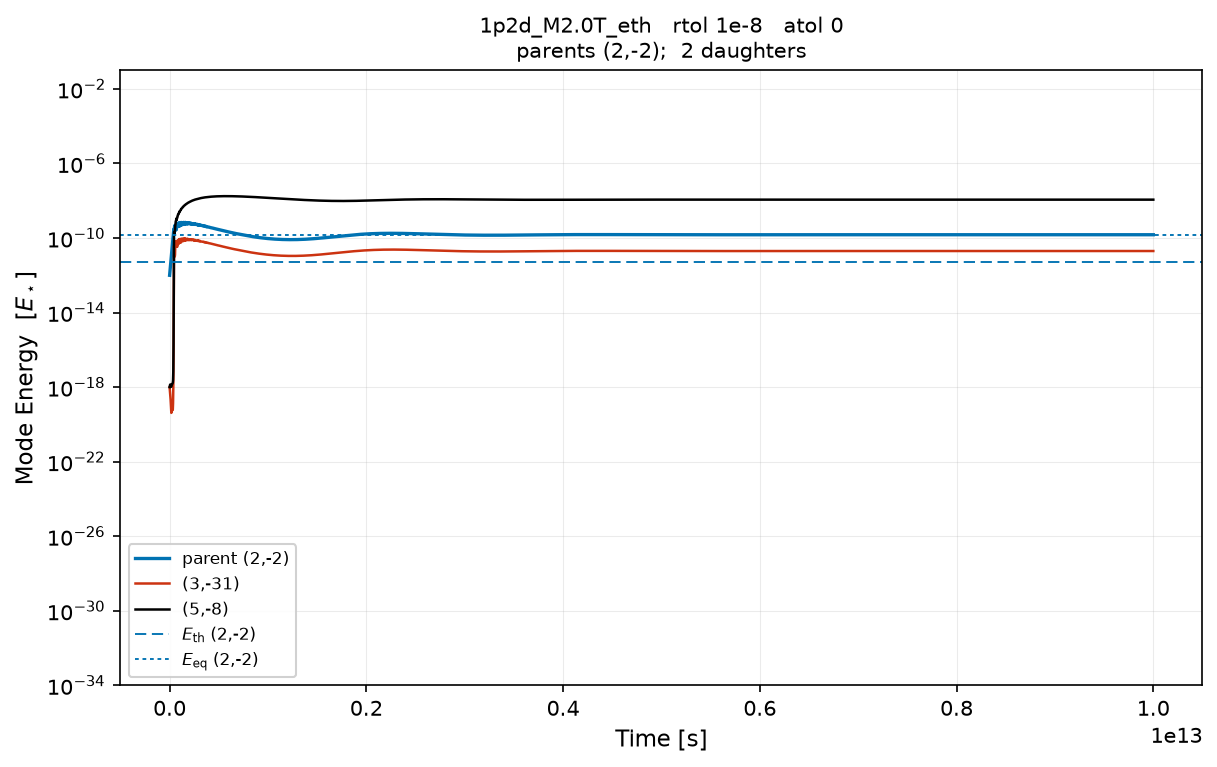
\includegraphics[width=0.21\textwidth,height=0.1323\textwidth]{../plots/rk8pd/1p2d_M2.0T_eth/r1e-8_a0.png} \\[-1pt]
 & \parbox[t]{0.21\textwidth}{\centering\scriptsize 385.4\,k steps, 0.4\,s} & \parbox[t]{0.21\textwidth}{\centering\scriptsize 385.4\,k steps, 0.6\,s} & \parbox[t]{0.21\textwidth}{\centering\scriptsize 385.4\,k steps, 0.8\,s} & \parbox[t]{0.21\textwidth}{\centering\scriptsize 385.4\,k steps, 0.9\,s} \\[2pt]
\rotatebox{90}{\parbox{0.1323\textwidth}{\centering\scriptsize\bfseries BDF, dense analytic Jacobian}} & 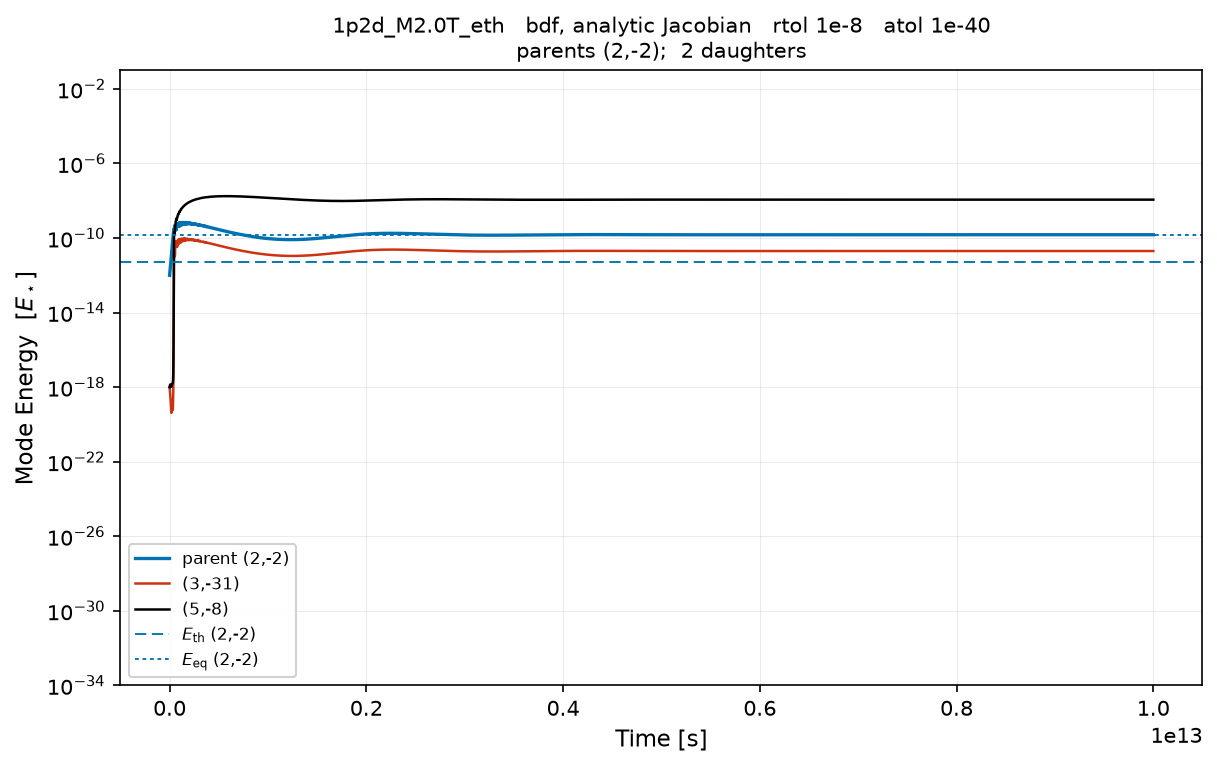
\includegraphics[width=0.21\textwidth,height=0.1323\textwidth]{../plots/bdf/1p2d_M2.0T_eth/r1e-8_a1e-40.png} & 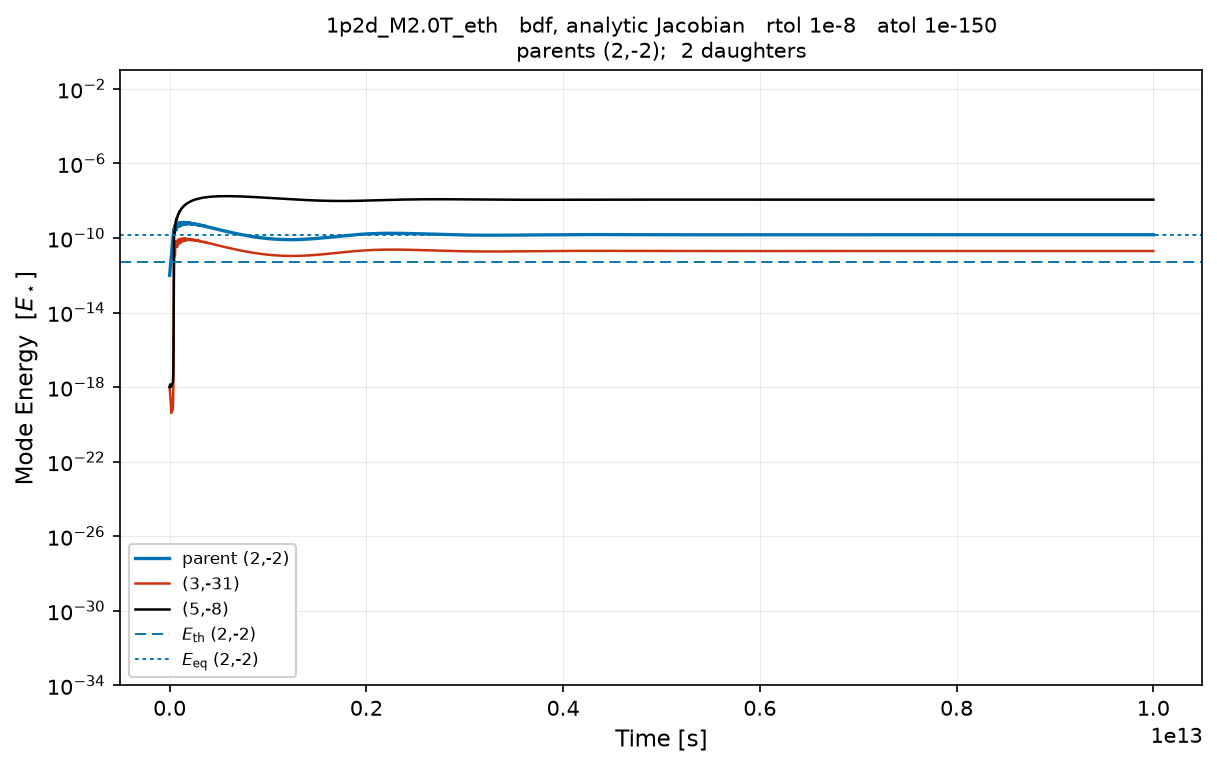
\includegraphics[width=0.21\textwidth,height=0.1323\textwidth]{../plots/bdf/1p2d_M2.0T_eth/r1e-8_a1e-150.png} & 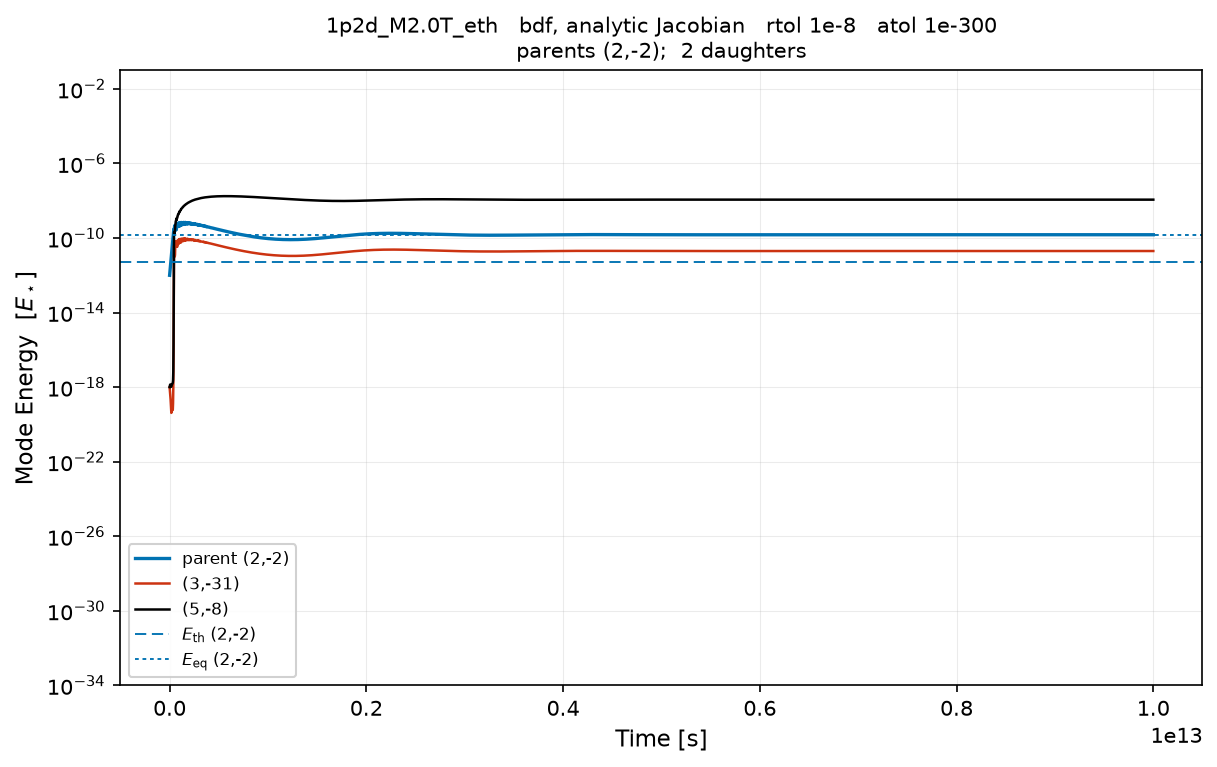
\includegraphics[width=0.21\textwidth,height=0.1323\textwidth]{../plots/bdf/1p2d_M2.0T_eth/r1e-8_a1e-300.png} & 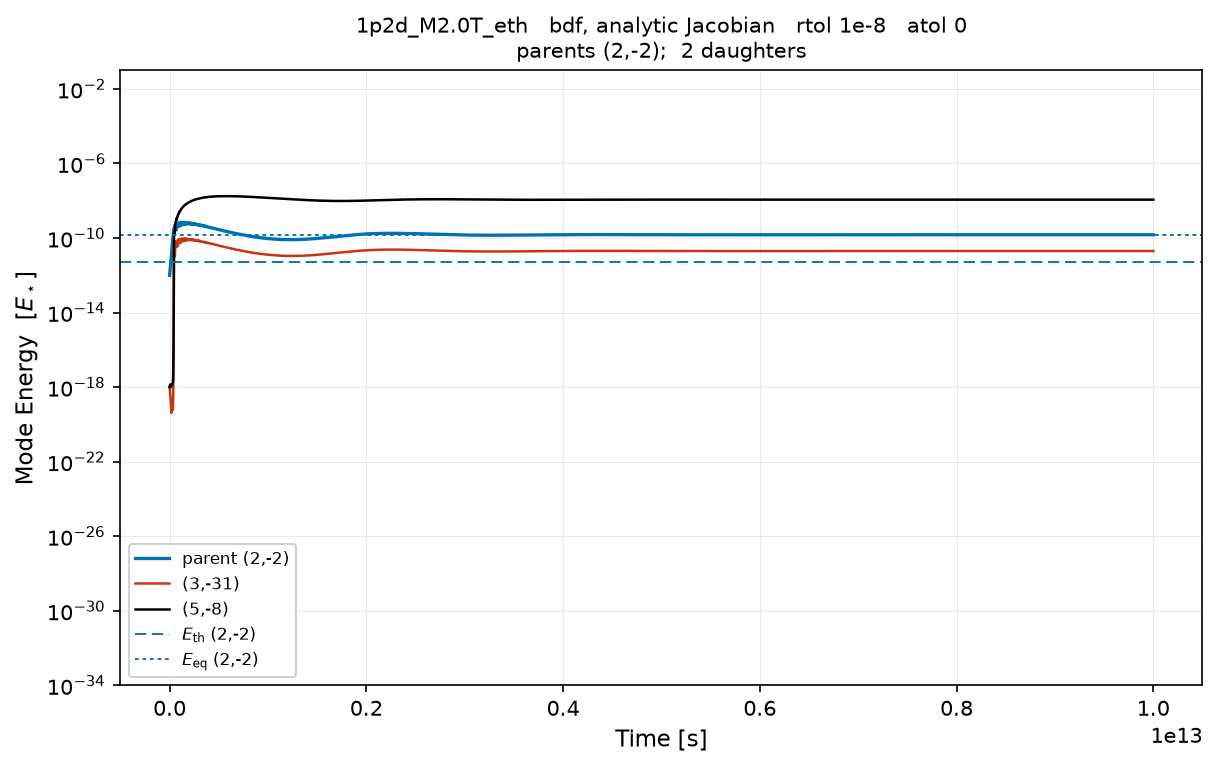
\includegraphics[width=0.21\textwidth,height=0.1323\textwidth]{../plots/bdf/1p2d_M2.0T_eth/r1e-8_a0.png} \\[-1pt]
 & \parbox[t]{0.21\textwidth}{\centering\scriptsize 3.60\,M steps, 3.8\,s} & \parbox[t]{0.21\textwidth}{\centering\scriptsize 3.60\,M steps, 2.5\,s} & \parbox[t]{0.21\textwidth}{\centering\scriptsize 3.60\,M steps, 4.9\,s} & \parbox[t]{0.21\textwidth}{\centering\scriptsize 3.60\,M steps, 2.8\,s} \\[2pt]
\rotatebox{90}{\parbox{0.1323\textwidth}{\centering\scriptsize\bfseries BDF-Krylov, band full}} & 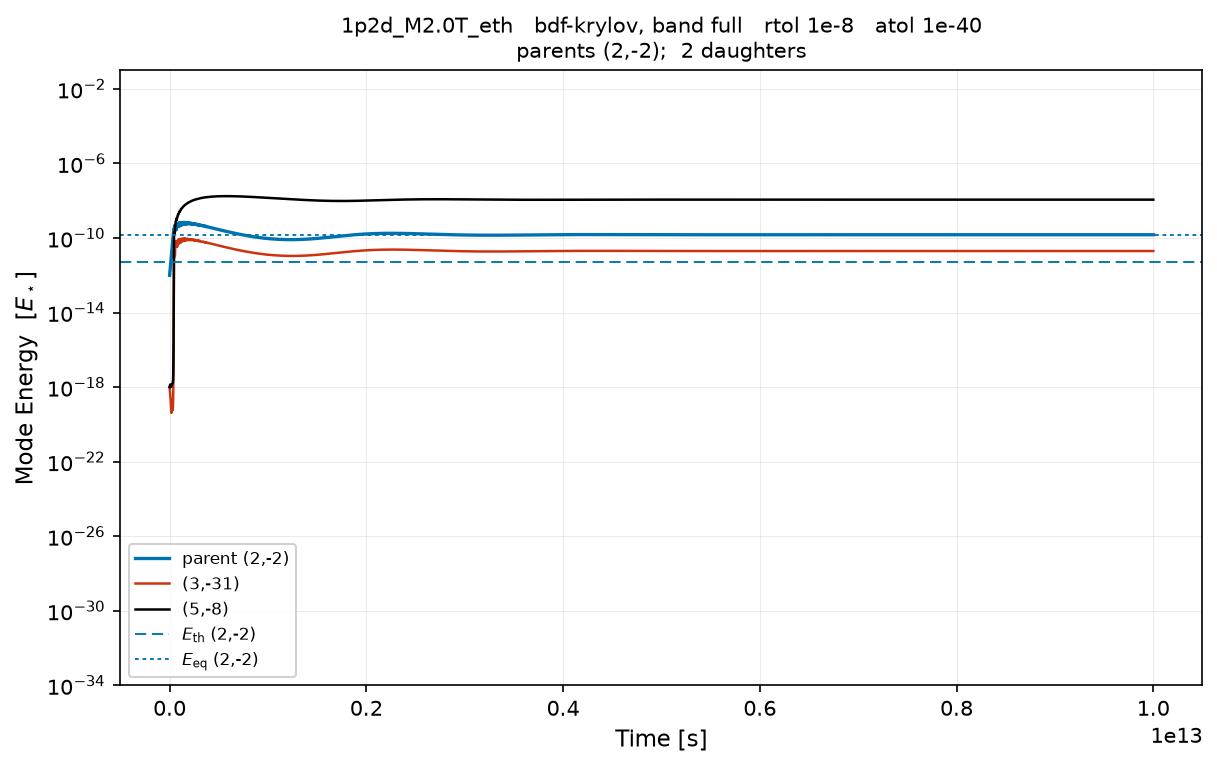
\includegraphics[width=0.21\textwidth,height=0.1323\textwidth]{../plots/krylov_full/1p2d_M2.0T_eth/r1e-8_a1e-40.png} & 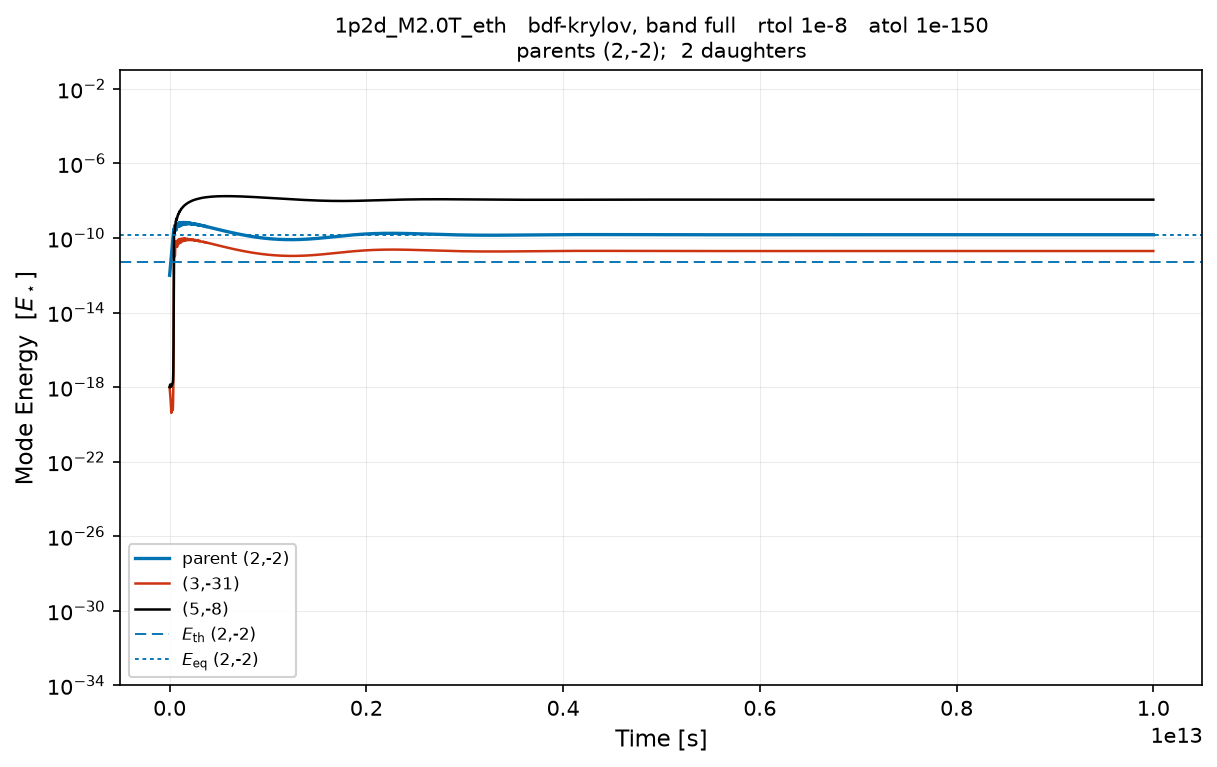
\includegraphics[width=0.21\textwidth,height=0.1323\textwidth]{../plots/krylov_full/1p2d_M2.0T_eth/r1e-8_a1e-150.png} & 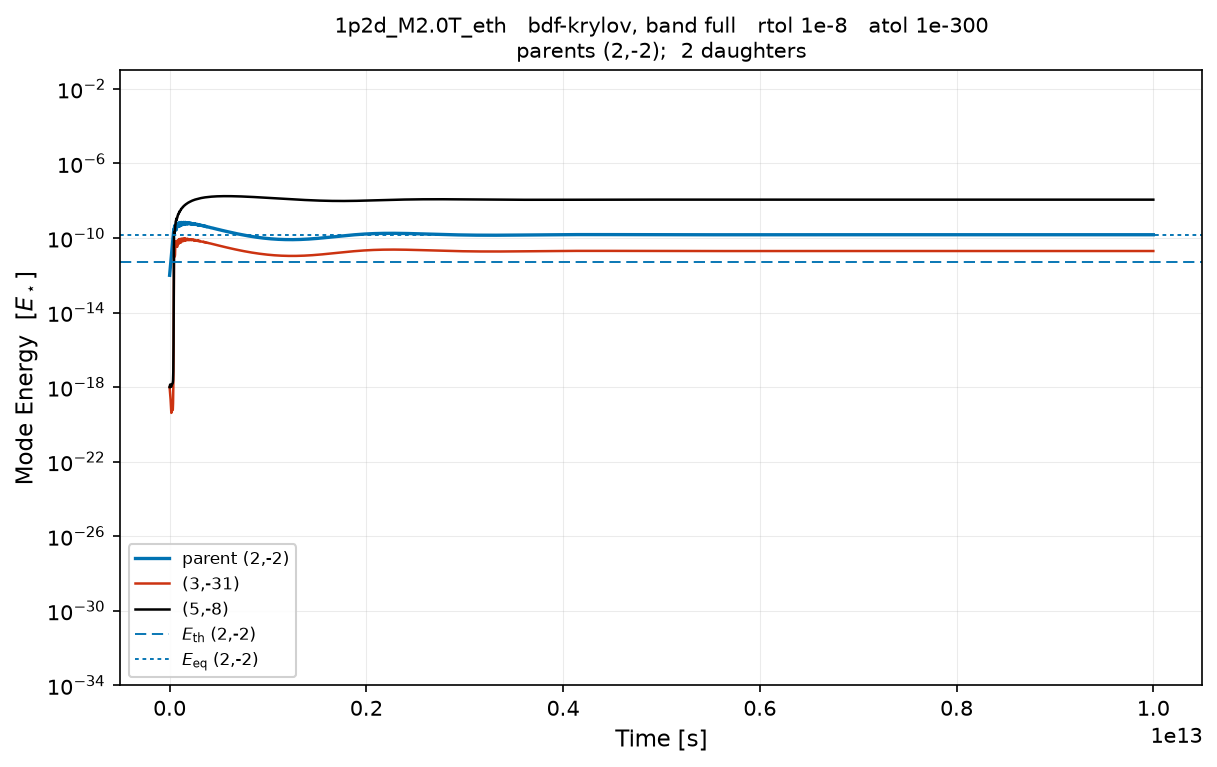
\includegraphics[width=0.21\textwidth,height=0.1323\textwidth]{../plots/krylov_full/1p2d_M2.0T_eth/r1e-8_a1e-300.png} & 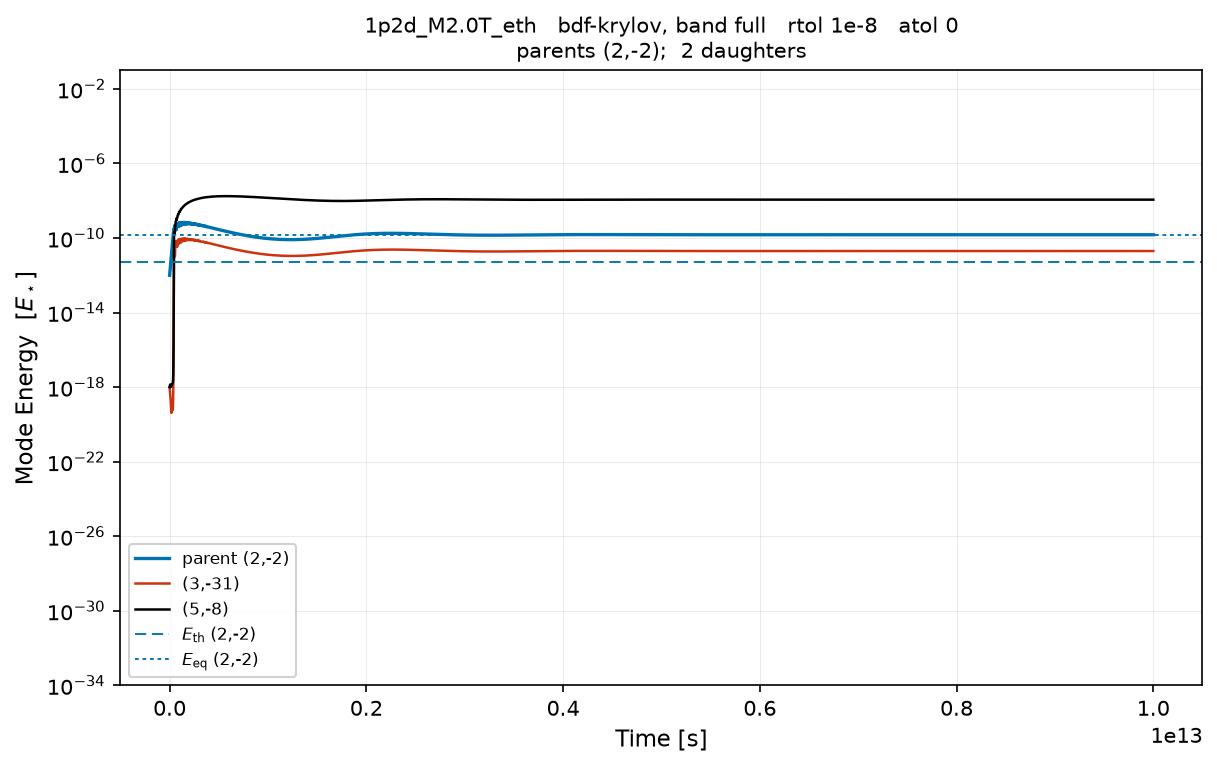
\includegraphics[width=0.21\textwidth,height=0.1323\textwidth]{../plots/krylov_full/1p2d_M2.0T_eth/r1e-8_a0.png} \\[-1pt]
 & \parbox[t]{0.21\textwidth}{\centering\scriptsize 3.55\,M steps, 6.6\,s} & \parbox[t]{0.21\textwidth}{\centering\scriptsize 3.55\,M steps, 4.2\,s} & \parbox[t]{0.21\textwidth}{\centering\scriptsize 3.55\,M steps, 6.6\,s} & \parbox[t]{0.21\textwidth}{\centering\scriptsize 3.55\,M steps, 6.9\,s} \\[2pt]
\rotatebox{90}{\parbox{0.1323\textwidth}{\centering\scriptsize\bfseries BDF-Krylov, band 3}} & 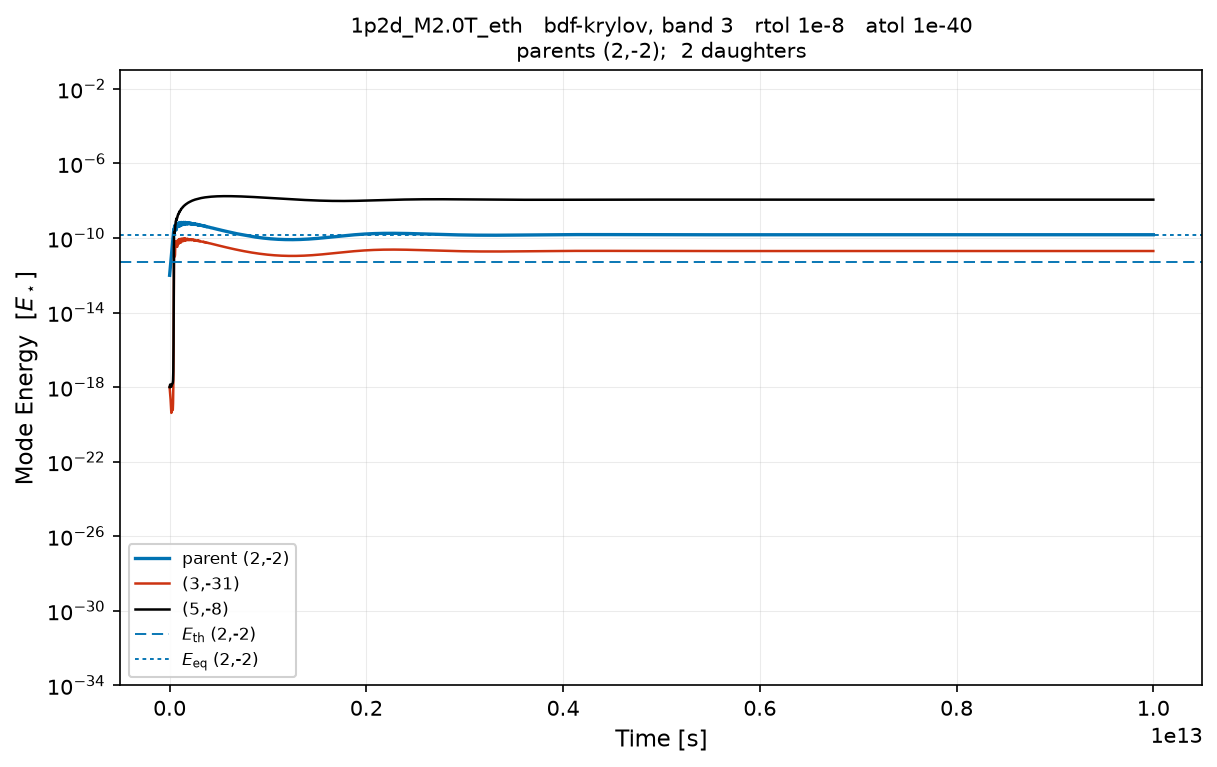
\includegraphics[width=0.21\textwidth,height=0.1323\textwidth]{../plots/krylov_b3/1p2d_M2.0T_eth/r1e-8_a1e-40.png} & 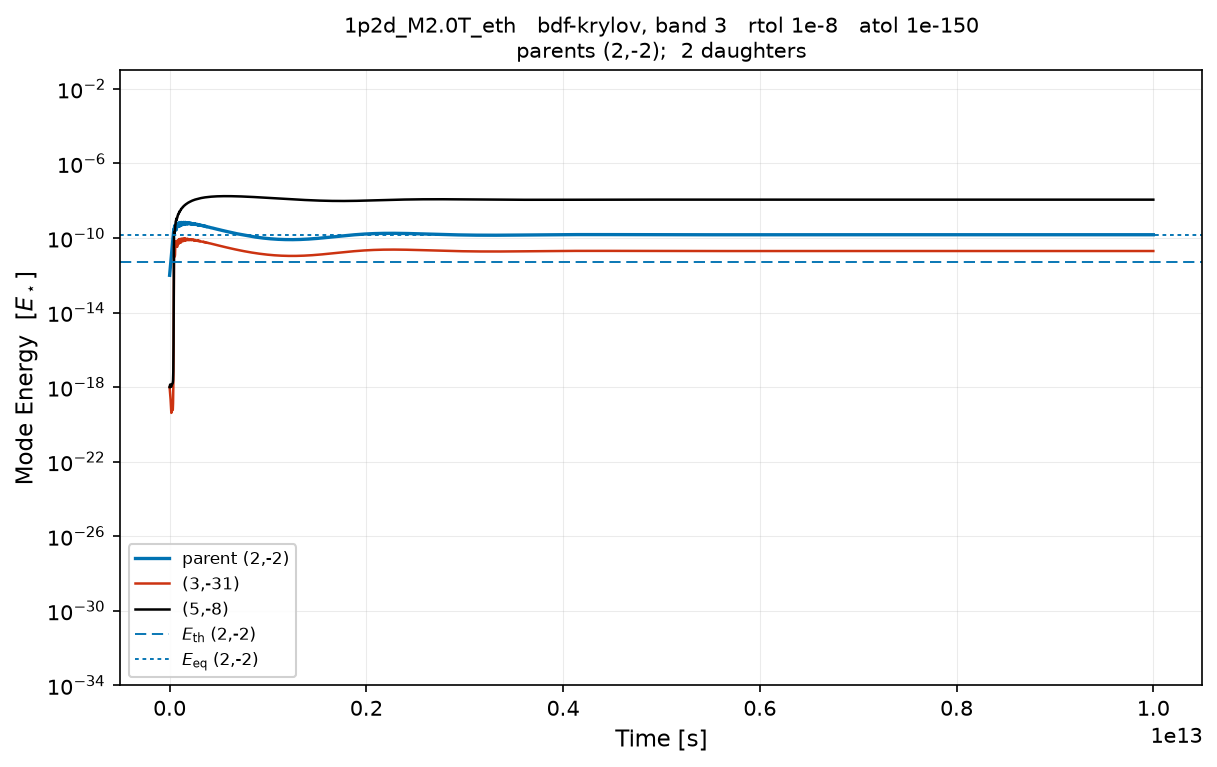
\includegraphics[width=0.21\textwidth,height=0.1323\textwidth]{../plots/krylov_b3/1p2d_M2.0T_eth/r1e-8_a1e-150.png} & 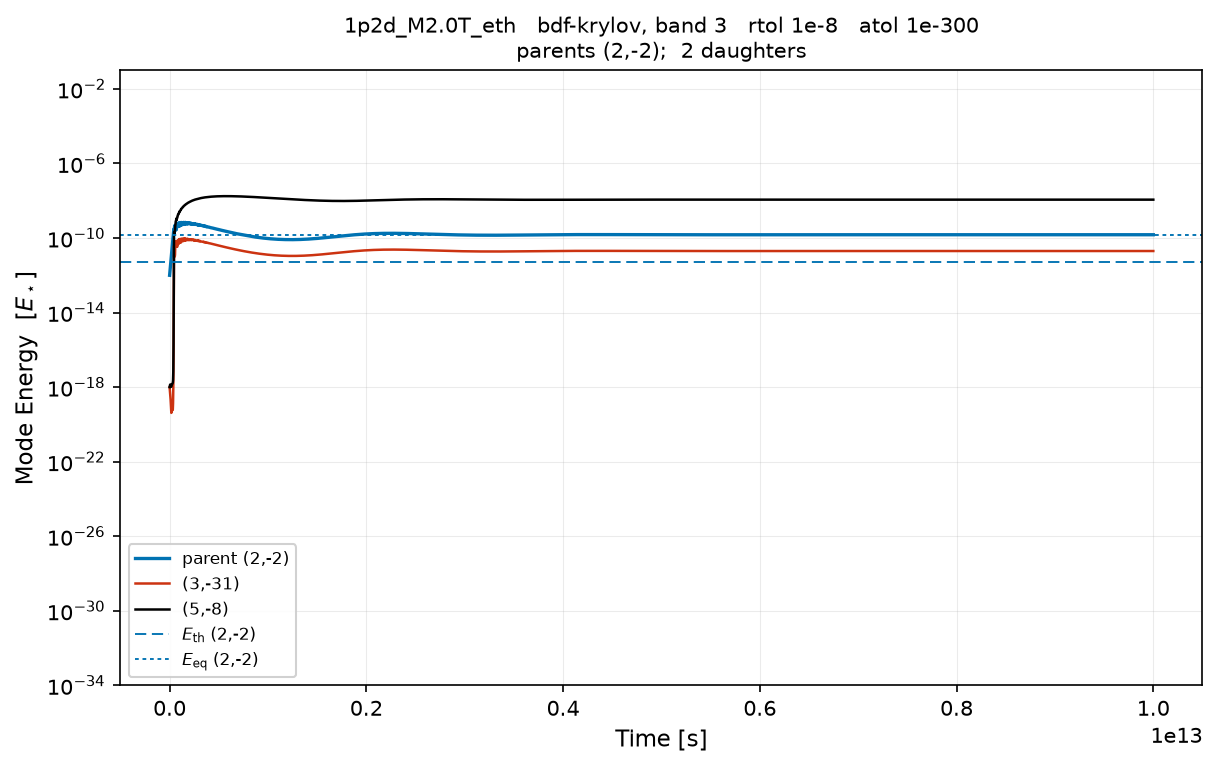
\includegraphics[width=0.21\textwidth,height=0.1323\textwidth]{../plots/krylov_b3/1p2d_M2.0T_eth/r1e-8_a1e-300.png} & 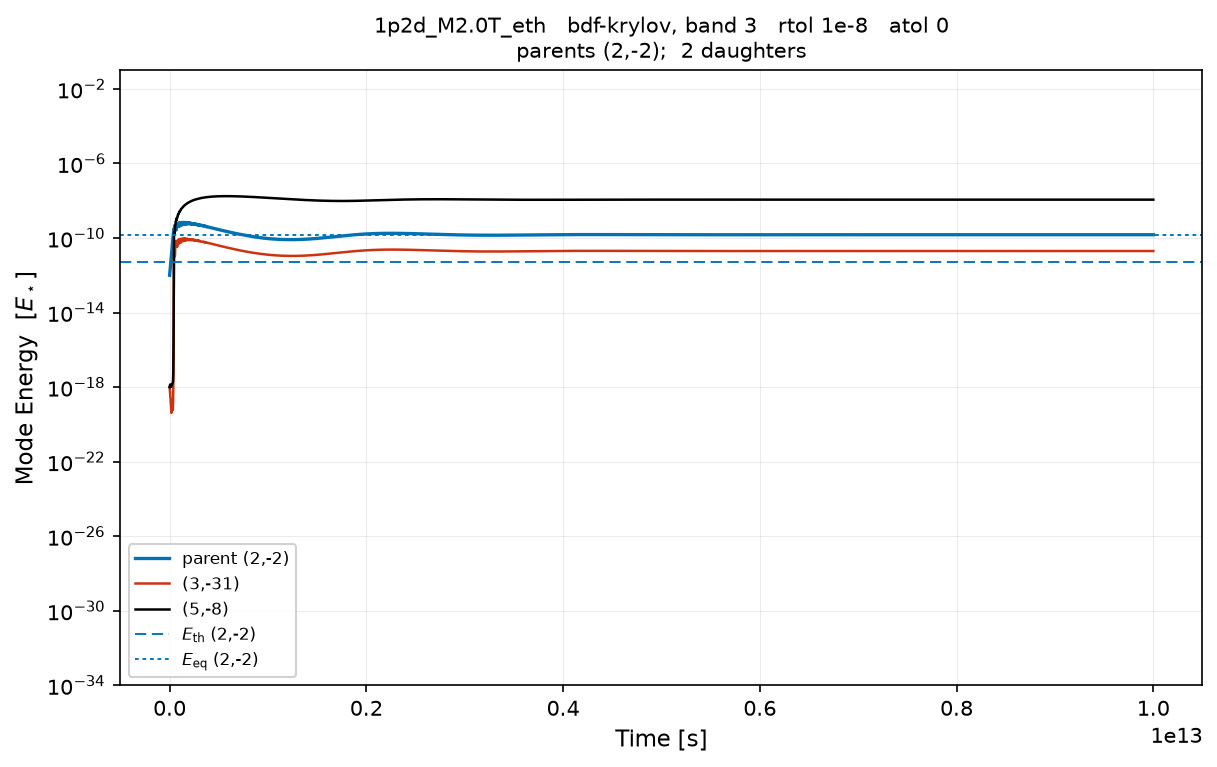
\includegraphics[width=0.21\textwidth,height=0.1323\textwidth]{../plots/krylov_b3/1p2d_M2.0T_eth/r1e-8_a0.png} \\[-1pt]
 & \parbox[t]{0.21\textwidth}{\centering\scriptsize 3.54\,M steps, 4.4\,s} & \parbox[t]{0.21\textwidth}{\centering\scriptsize 3.54\,M steps, 6.8\,s} & \parbox[t]{0.21\textwidth}{\centering\scriptsize 3.54\,M steps, 6.5\,s} & \parbox[t]{0.21\textwidth}{\centering\scriptsize 3.54\,M steps, 6.8\,s} \\[2pt]
\rotatebox{90}{\parbox{0.1323\textwidth}{\centering\scriptsize\bfseries Adams, fixed point}} & 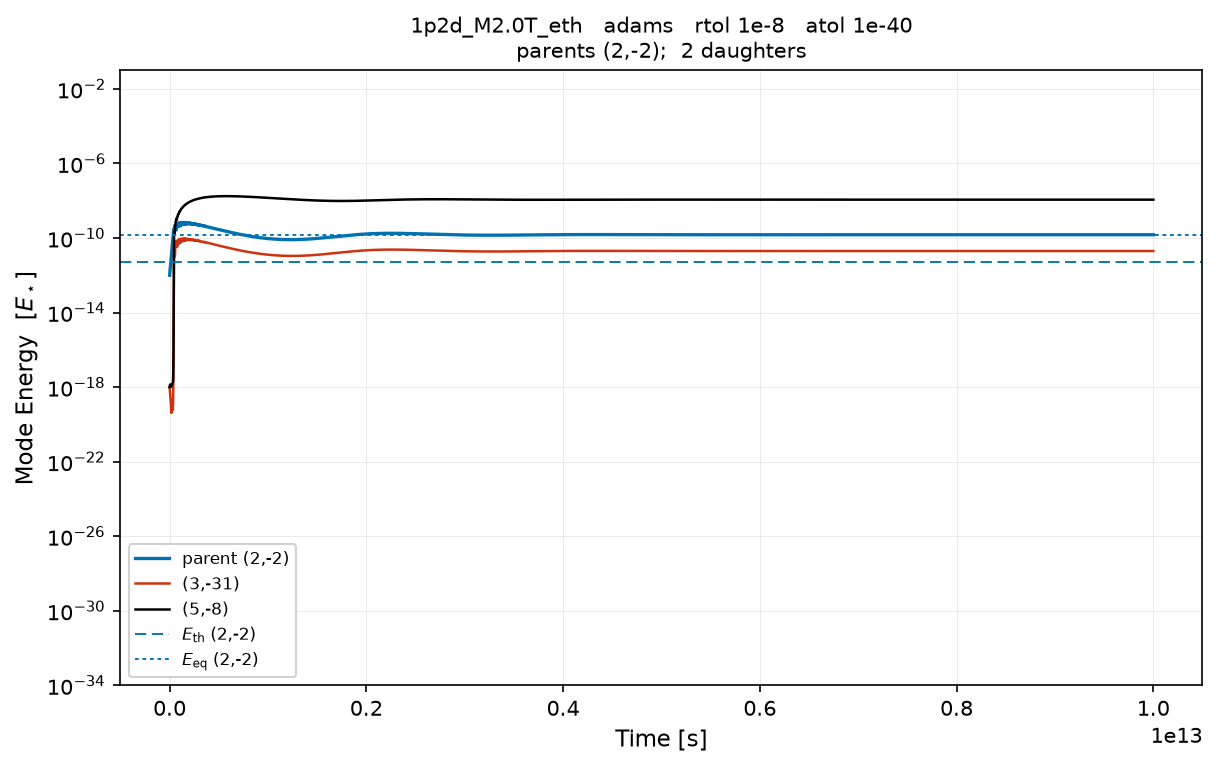
\includegraphics[width=0.21\textwidth,height=0.1323\textwidth]{../plots/adams/1p2d_M2.0T_eth/r1e-8_a1e-40.png} & 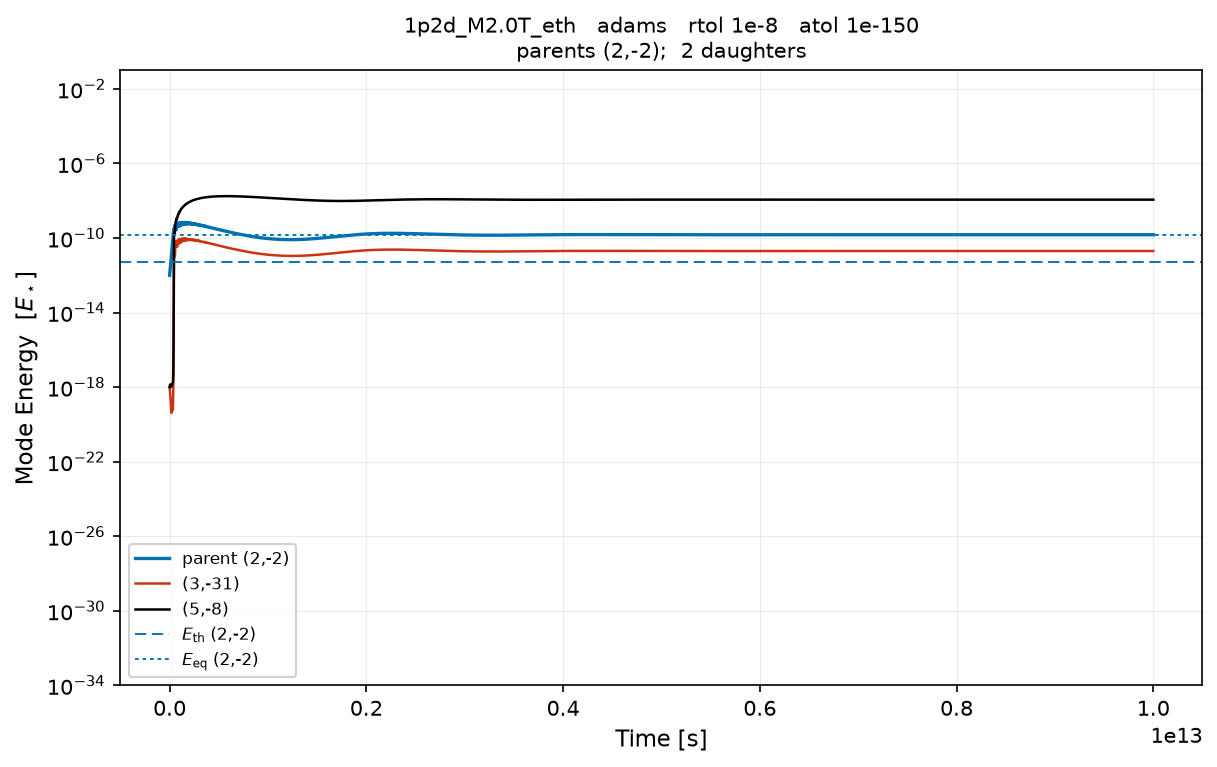
\includegraphics[width=0.21\textwidth,height=0.1323\textwidth]{../plots/adams/1p2d_M2.0T_eth/r1e-8_a1e-150.png} & 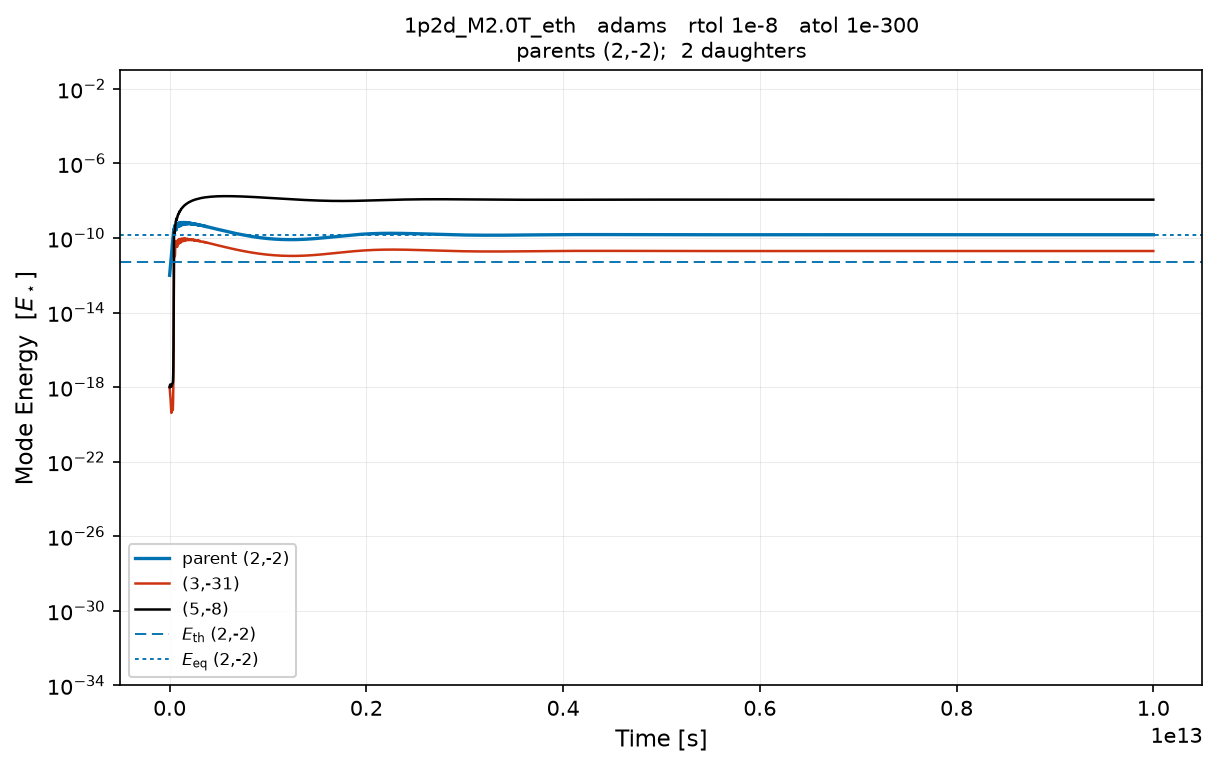
\includegraphics[width=0.21\textwidth,height=0.1323\textwidth]{../plots/adams/1p2d_M2.0T_eth/r1e-8_a1e-300.png} & 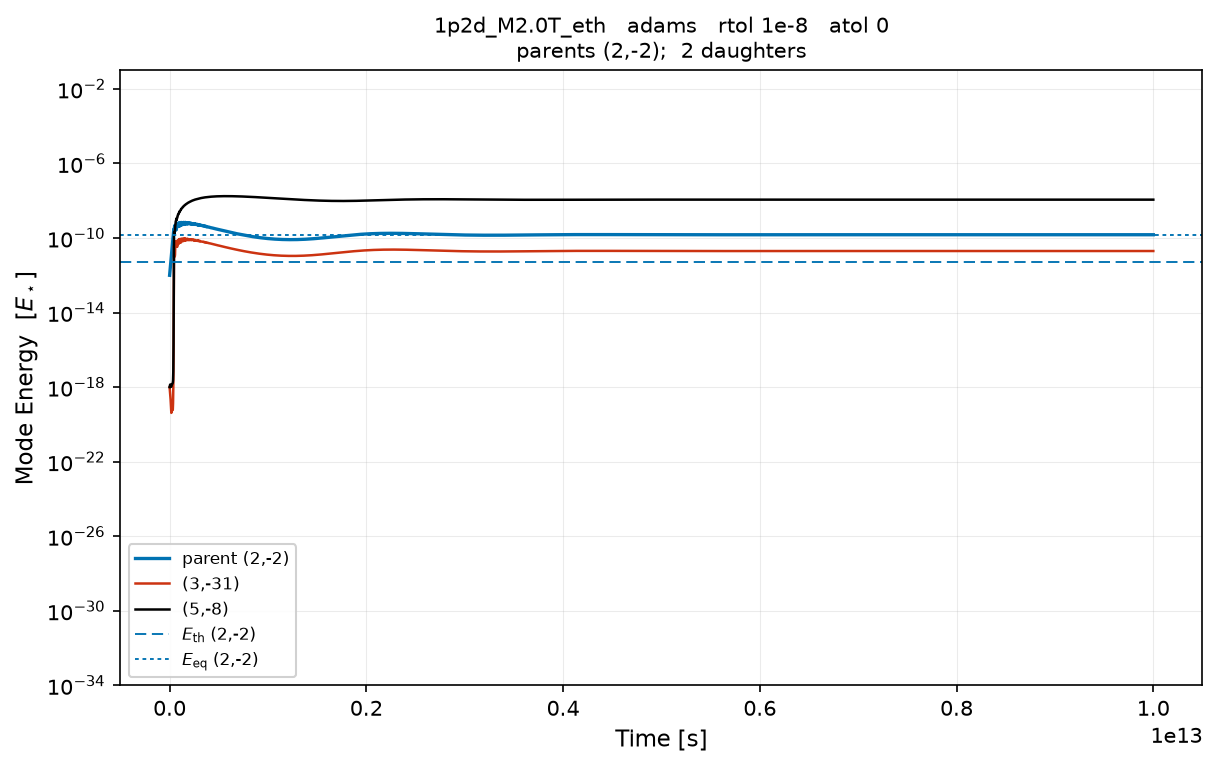
\includegraphics[width=0.21\textwidth,height=0.1323\textwidth]{../plots/adams/1p2d_M2.0T_eth/r1e-8_a0.png} \\[-1pt]
 & \parbox[t]{0.21\textwidth}{\centering\scriptsize 2.04\,M steps, 2.6\,s} & \parbox[t]{0.21\textwidth}{\centering\scriptsize 2.04\,M steps, 2.6\,s} & \parbox[t]{0.21\textwidth}{\centering\scriptsize 2.04\,M steps, 2.6\,s} & \parbox[t]{0.21\textwidth}{\centering\scriptsize 2.04\,M steps, 2.6\,s} \\[2pt]
\end{tabular}\par}
\par\noindent{\scriptsize\setlength\tabcolsep{3.5pt}\renewcommand\arraystretch{0.92}
\begin{tabular}{@{}llllrrrrrrr@{}}
\toprule
integrator & atol & stop & $t_{\rm stop}$ [s] & steps & rejected & RHS & Jac. & NL it. & lin. it. & wall [s] \\
\midrule
rk8pd & $10^{-40}$ & end & $1.00\times10^{13}$ & 385.4\,k & 83.7\,k & 5.01\,M & -- & -- & -- & 0.4 \\
 & $10^{-150}$ & end & $1.00\times10^{13}$ & 385.4\,k & 83.7\,k & 5.01\,M & -- & -- & -- & 0.6 \\
 & $10^{-300}$ & end & $1.00\times10^{13}$ & 385.4\,k & 83.7\,k & 5.01\,M & -- & -- & -- & 0.8 \\
 & $0$ & end & $1.00\times10^{13}$ & 385.4\,k & 83.7\,k & 5.01\,M & -- & -- & -- & 0.9 \\
\addlinespace[2pt]
BDF, dense analytic Jacobian & $10^{-40}$ & end & $1.00\times10^{13}$ & 3.60\,M & 59.0\,k & 3.99\,M & 77.3\,k & 3.99\,M & -- & 3.8 \\
 & $10^{-150}$ & end & $1.00\times10^{13}$ & 3.60\,M & 59.0\,k & 3.99\,M & 77.3\,k & 3.99\,M & -- & 2.5 \\
 & $10^{-300}$ & end & $1.00\times10^{13}$ & 3.60\,M & 59.0\,k & 3.99\,M & 77.3\,k & 3.99\,M & -- & 4.9 \\
 & $0$ & end & $1.00\times10^{13}$ & 3.60\,M & 59.0\,k & 3.99\,M & 77.3\,k & 3.99\,M & -- & 2.8 \\
\addlinespace[2pt]
BDF-Krylov, band full & $10^{-40}$ & end & $1.00\times10^{13}$ & 3.55\,M & 60.9\,k & 7.98\,M & 73.4\,k & 3.91\,M & 3.62\,M & 6.6 \\
 & $10^{-150}$ & end & $1.00\times10^{13}$ & 3.55\,M & 60.9\,k & 7.98\,M & 73.4\,k & 3.91\,M & 3.62\,M & 4.2 \\
 & $10^{-300}$ & end & $1.00\times10^{13}$ & 3.55\,M & 60.9\,k & 7.98\,M & 73.4\,k & 3.91\,M & 3.62\,M & 6.6 \\
 & $0$ & end & $1.00\times10^{13}$ & 3.55\,M & 60.9\,k & 7.98\,M & 73.4\,k & 3.91\,M & 3.62\,M & 6.9 \\
\addlinespace[2pt]
BDF-Krylov, band 3 & $10^{-40}$ & end & $1.00\times10^{13}$ & 3.54\,M & 61.1\,k & 7.98\,M & 73.2\,k & 3.91\,M & 3.63\,M & 4.4 \\
 & $10^{-150}$ & end & $1.00\times10^{13}$ & 3.54\,M & 61.1\,k & 7.98\,M & 73.2\,k & 3.91\,M & 3.63\,M & 6.8 \\
 & $10^{-300}$ & end & $1.00\times10^{13}$ & 3.54\,M & 61.1\,k & 7.98\,M & 73.2\,k & 3.91\,M & 3.63\,M & 6.5 \\
 & $0$ & end & $1.00\times10^{13}$ & 3.54\,M & 61.1\,k & 7.98\,M & 73.2\,k & 3.91\,M & 3.63\,M & 6.8 \\
\addlinespace[2pt]
Adams, fixed point & $10^{-40}$ & end & $1.00\times10^{13}$ & 2.04\,M & 134.1\,k & 3.35\,M & -- & 3.34\,M & -- & 2.6 \\
 & $10^{-150}$ & end & $1.00\times10^{13}$ & 2.04\,M & 134.1\,k & 3.35\,M & -- & 3.34\,M & -- & 2.6 \\
 & $10^{-300}$ & end & $1.00\times10^{13}$ & 2.04\,M & 134.1\,k & 3.35\,M & -- & 3.34\,M & -- & 2.6 \\
 & $0$ & end & $1.00\times10^{13}$ & 2.04\,M & 134.1\,k & 3.35\,M & -- & 3.34\,M & -- & 2.6 \\
\bottomrule
\end{tabular}}

\clearpage
\subsection{\texttt{1p2d\_M2.0\_dgamma}}\label{net:1p2d_M2.0_dgamma}
\noindent\begin{minipage}[t]{0.43\textwidth}\vspace{0pt}\footnotesize
\begin{tabular}{@{}rrlrr@{}}
\toprule
id & gen & $(\ell,n)$ & $\omega$ [rad\,s$^{-1}$] & $\gamma$ [s$^{-1}$] \\
\midrule
0 & 0 & (1,$-$1) & $7.581\times10^{-4}$ & $-2.276\times10^{-10}$ \\
1 & 1 & (5,$-$9) & $6.198\times10^{-4}$ & $4.584\times10^{-13}$ \\
2 & 1 & (6,$-$56) & $1.377\times10^{-4}$ & $2.817\times10^{-9}$ \\
\bottomrule
\end{tabular}
\end{minipage}\hfill
\begin{minipage}[t]{0.55\textwidth}\vspace{0pt}\footnotesize
\textbf{Model} \texttt{dsct\_M2.0}, rule dgamma, $N=1$, cut 0.15,
closure 0.005; 3 modes, 1 triplet(s).\\[2pt]
\textbf{Selecting pairs}\\ (1,$-$1) $\to$ (5,$-$9) + (6,$-$56): $\Delta/\omega_a=-6.83\times10^{-4}$, $\kappa=+0.085$, $E_{\rm th}=1.75\times10^{-8}$, $E_{\rm eq}=2.07\times10^{-8}$\\[2pt]
Deep dips between bursts.
\end{minipage}

\par\smallskip{\centering\begin{tabular}{@{}c@{\hspace{2pt}}c@{\hspace{2pt}}c@{\hspace{2pt}}c@{\hspace{2pt}}c@{}}
 & \small atol $10^{-40}$ & \small atol $10^{-150}$ & \small atol $10^{-300}$ & \small atol $0$ \\[1pt]
\rotatebox{90}{\parbox{0.1323\textwidth}{\centering\scriptsize\bfseries rk8pd}} & 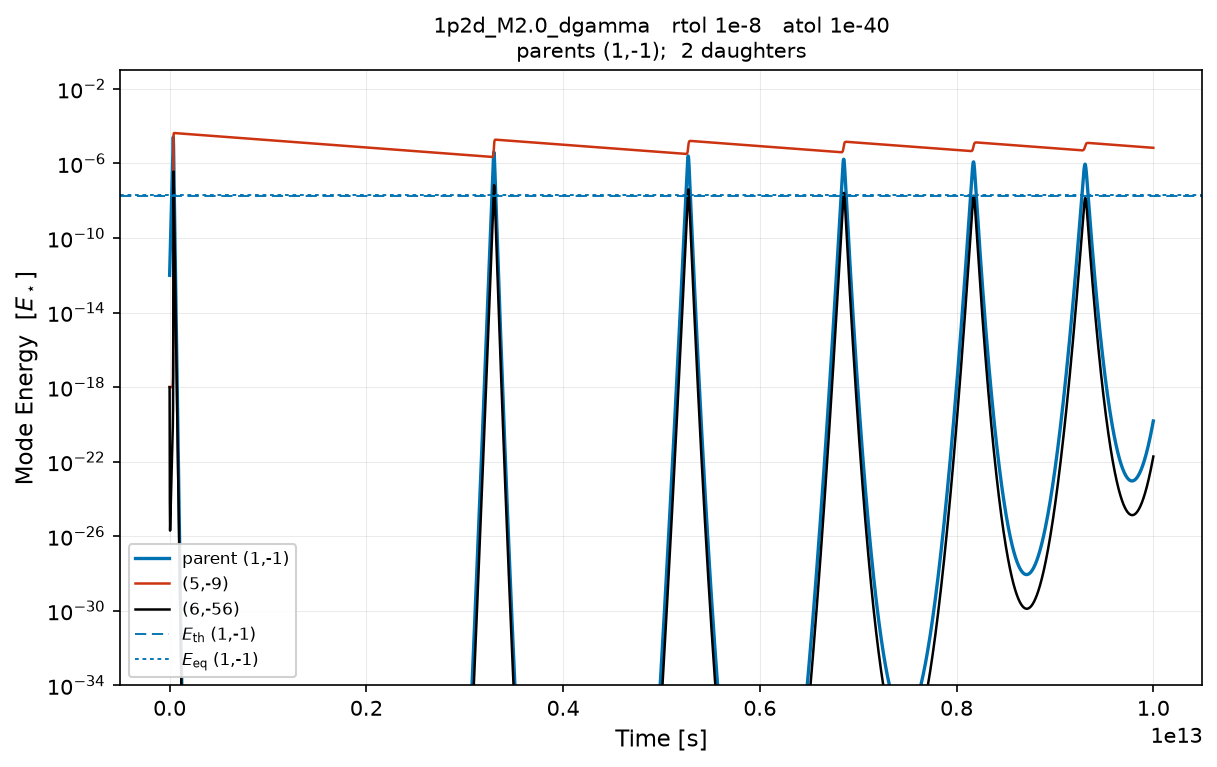
\includegraphics[width=0.21\textwidth,height=0.1323\textwidth]{../plots/rk8pd/1p2d_M2.0_dgamma/r1e-8_a1e-40.png} & 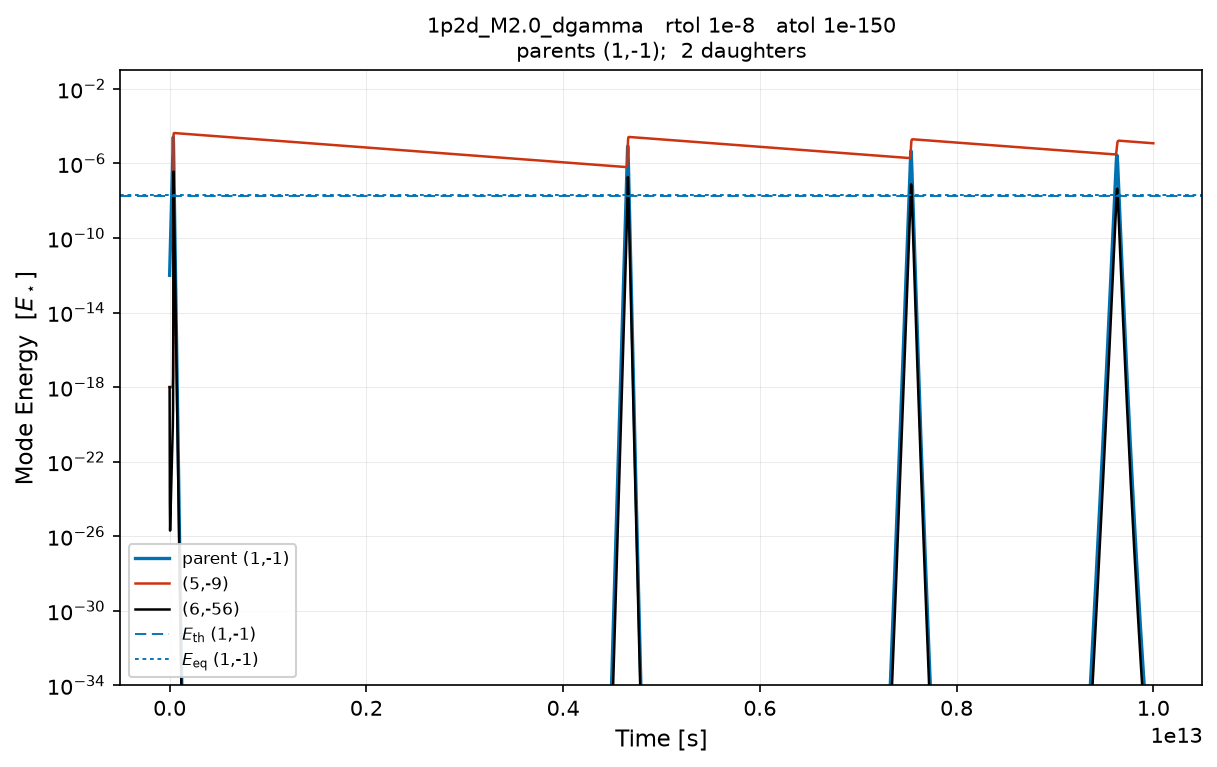
\includegraphics[width=0.21\textwidth,height=0.1323\textwidth]{../plots/rk8pd/1p2d_M2.0_dgamma/r1e-8_a1e-150.png} & 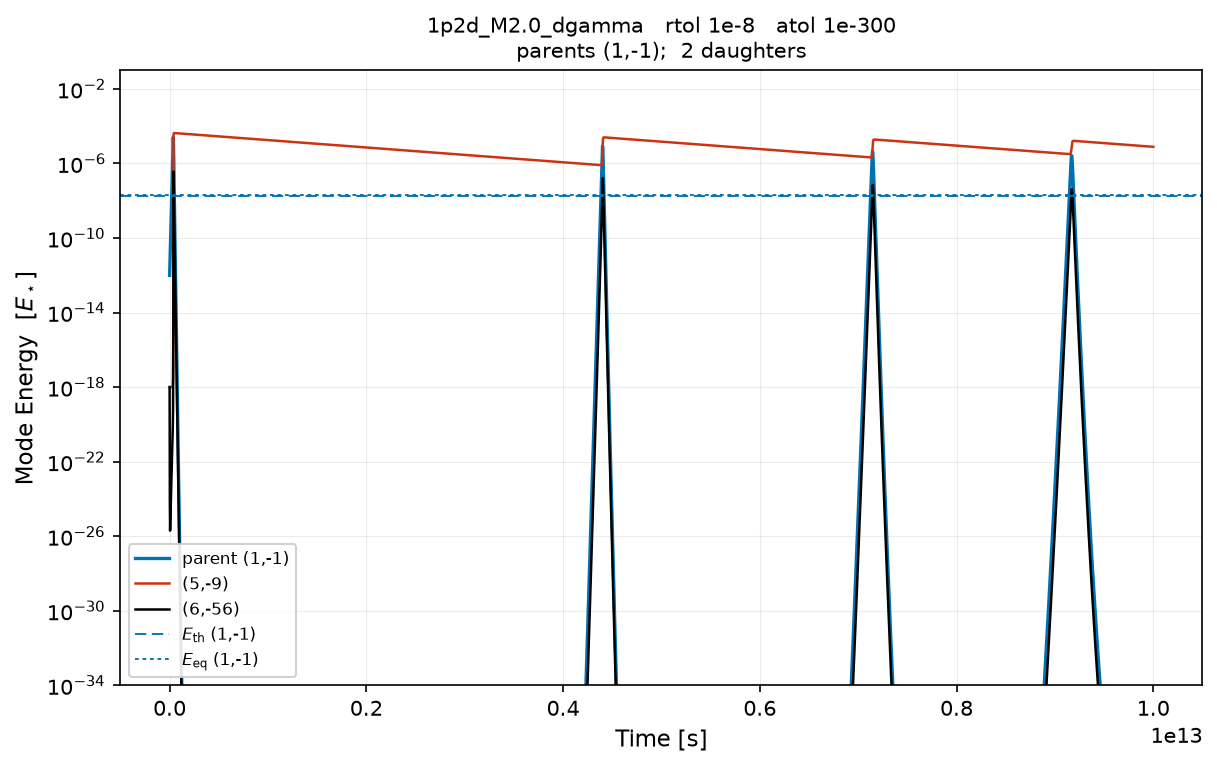
\includegraphics[width=0.21\textwidth,height=0.1323\textwidth]{../plots/rk8pd/1p2d_M2.0_dgamma/r1e-8_a1e-300.png} & 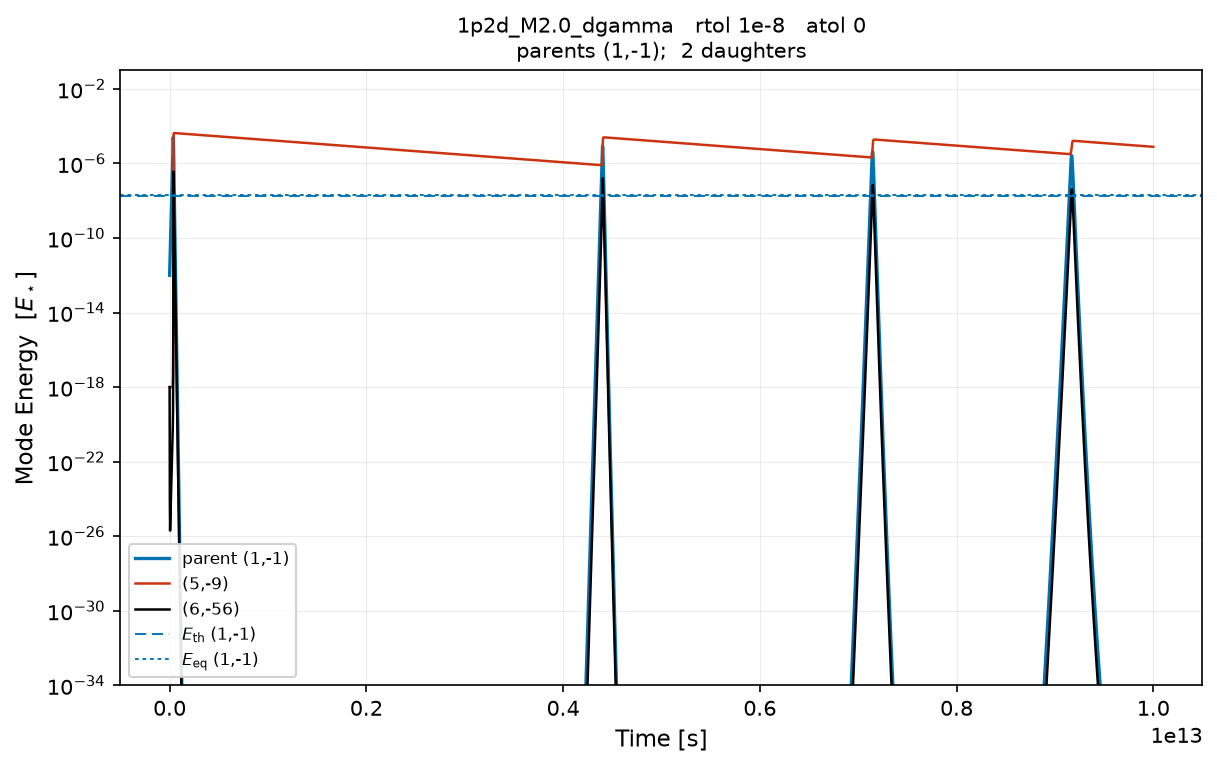
\includegraphics[width=0.21\textwidth,height=0.1323\textwidth]{../plots/rk8pd/1p2d_M2.0_dgamma/r1e-8_a0.png} \\[-1pt]
 & \parbox[t]{0.21\textwidth}{\centering\scriptsize 6.61\,M steps, 9.5\,s} & \parbox[t]{0.21\textwidth}{\centering\scriptsize 8.24\,M steps, 15.6\,s} & \parbox[t]{0.21\textwidth}{\centering\scriptsize 9.26\,M steps, 13.5\,s} & \parbox[t]{0.21\textwidth}{\centering\scriptsize 9.26\,M steps, 20.4\,s} \\[2pt]
\rotatebox{90}{\parbox{0.1323\textwidth}{\centering\scriptsize\bfseries BDF, dense analytic Jacobian}} & 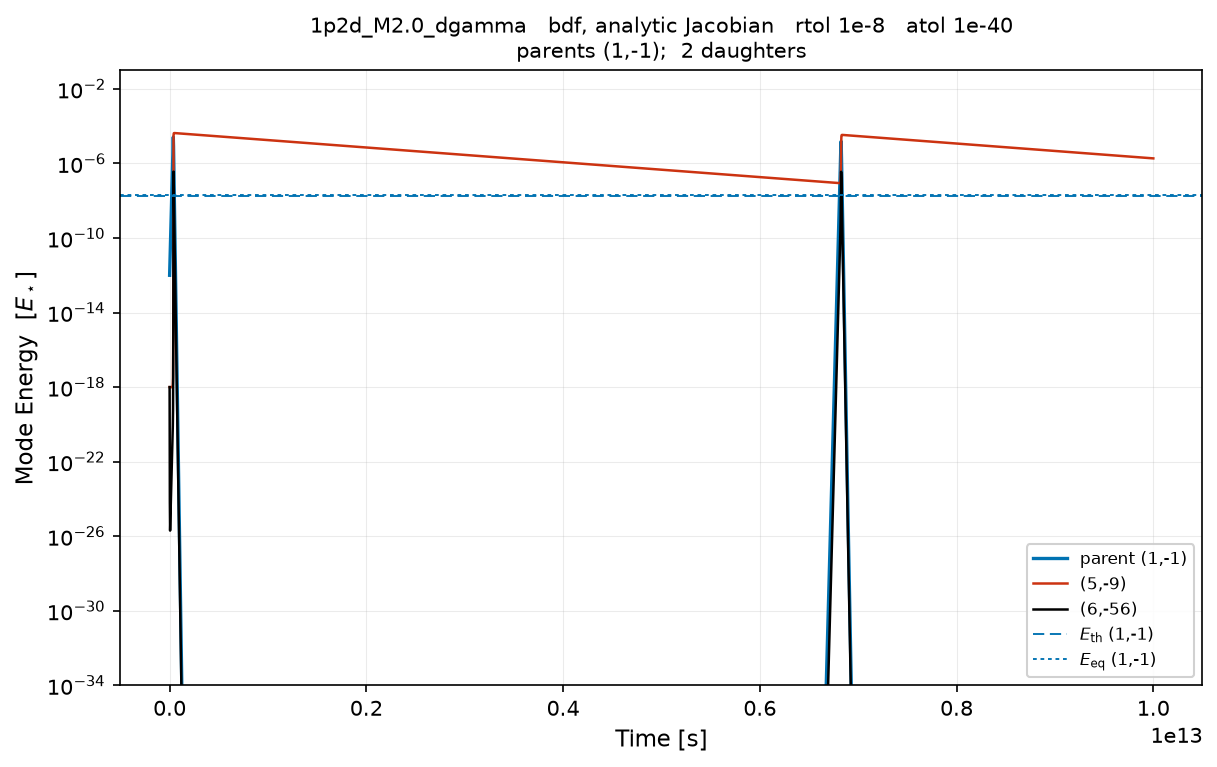
\includegraphics[width=0.21\textwidth,height=0.1323\textwidth]{../plots/bdf/1p2d_M2.0_dgamma/r1e-8_a1e-40.png} & 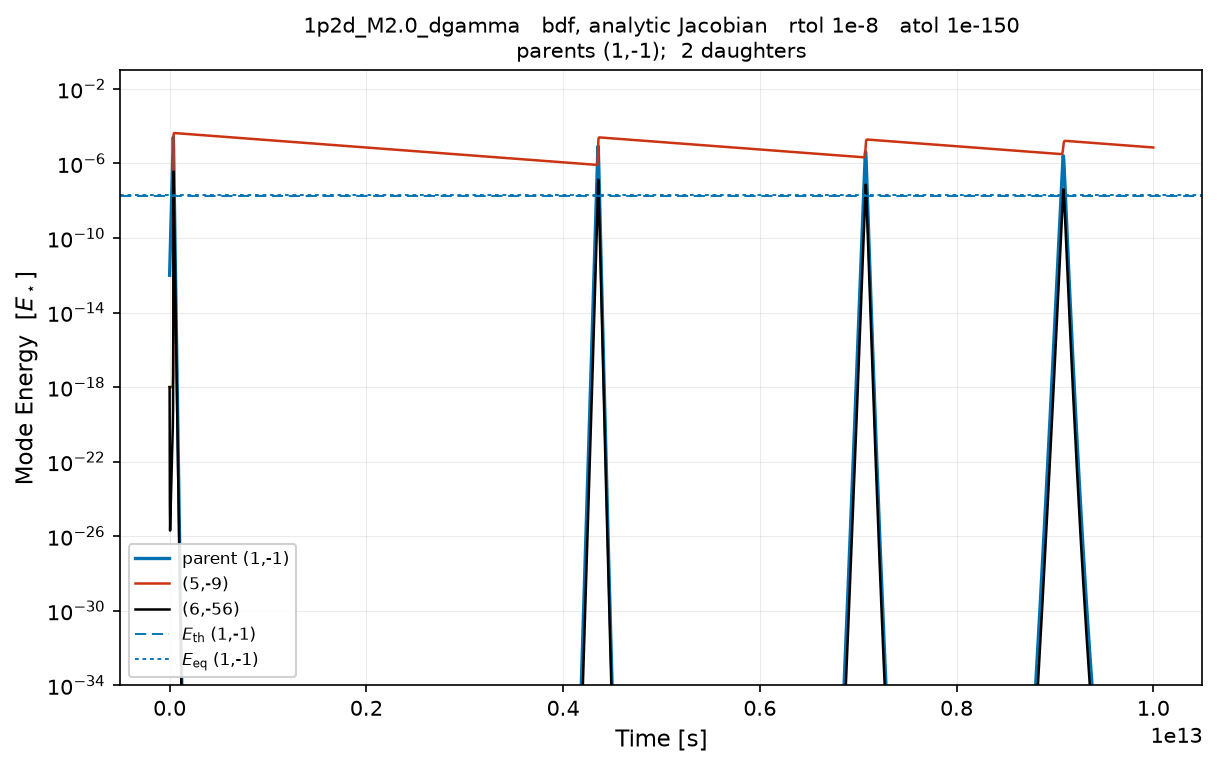
\includegraphics[width=0.21\textwidth,height=0.1323\textwidth]{../plots/bdf/1p2d_M2.0_dgamma/r1e-8_a1e-150.png} & 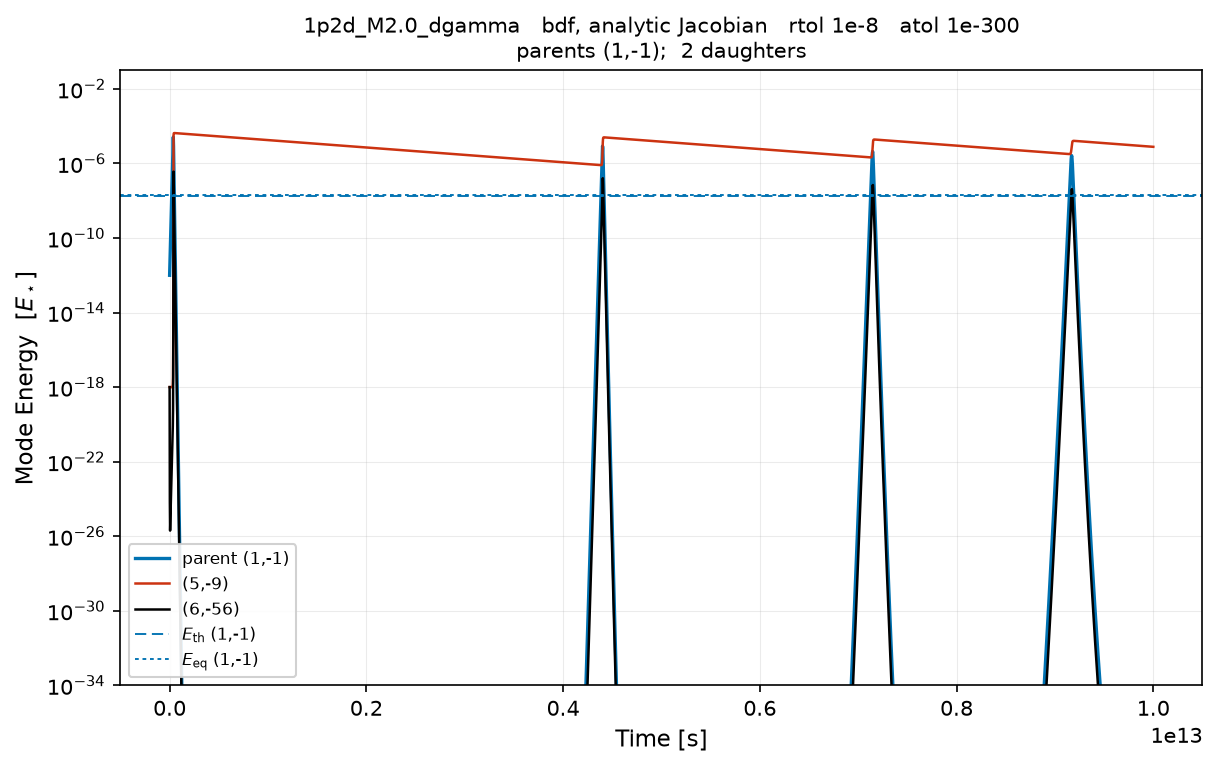
\includegraphics[width=0.21\textwidth,height=0.1323\textwidth]{../plots/bdf/1p2d_M2.0_dgamma/r1e-8_a1e-300.png} & 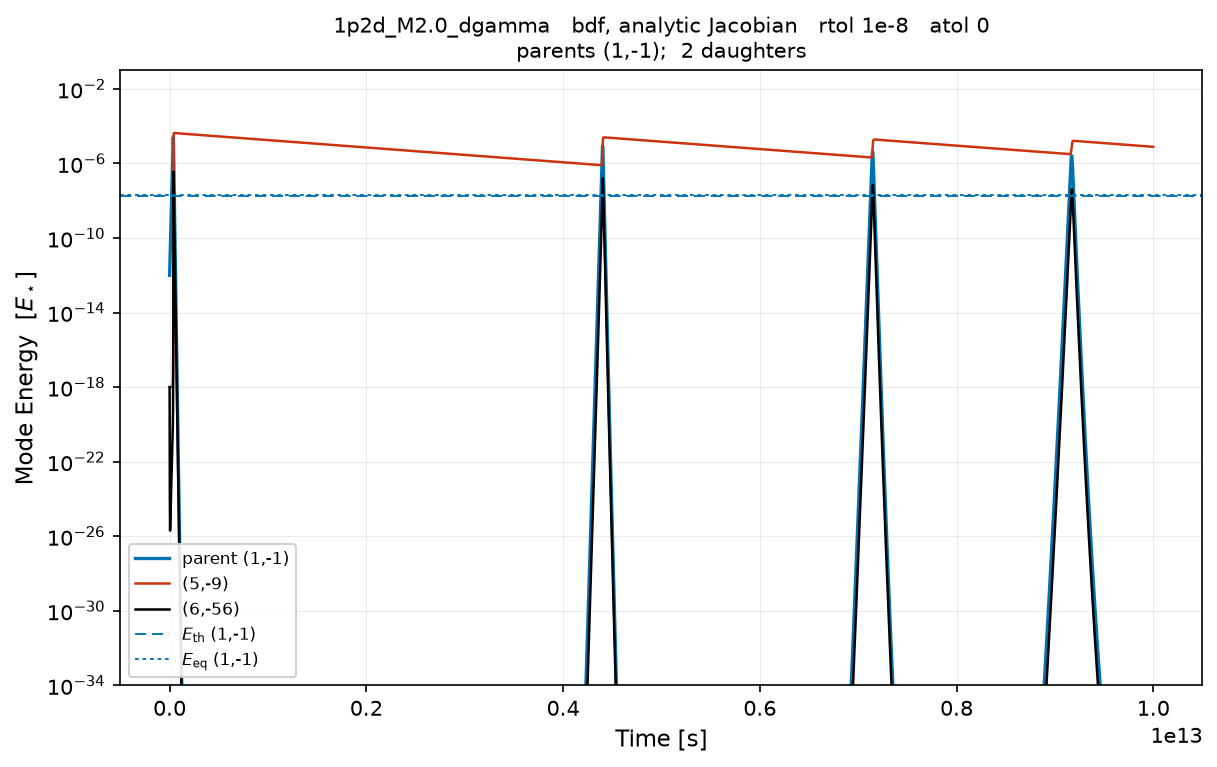
\includegraphics[width=0.21\textwidth,height=0.1323\textwidth]{../plots/bdf/1p2d_M2.0_dgamma/r1e-8_a0.png} \\[-1pt]
 & \parbox[t]{0.21\textwidth}{\centering\scriptsize 14.40\,M steps, 12.8\,s} & \parbox[t]{0.21\textwidth}{\centering\scriptsize 114.97\,M steps, 154.3\,s} & \parbox[t]{0.21\textwidth}{\centering\scriptsize 120.93\,M steps, 140.1\,s} & \parbox[t]{0.21\textwidth}{\centering\scriptsize 120.93\,M steps, 168.2\,s} \\[2pt]
\rotatebox{90}{\parbox{0.1323\textwidth}{\centering\scriptsize\bfseries BDF-Krylov, band full}} & 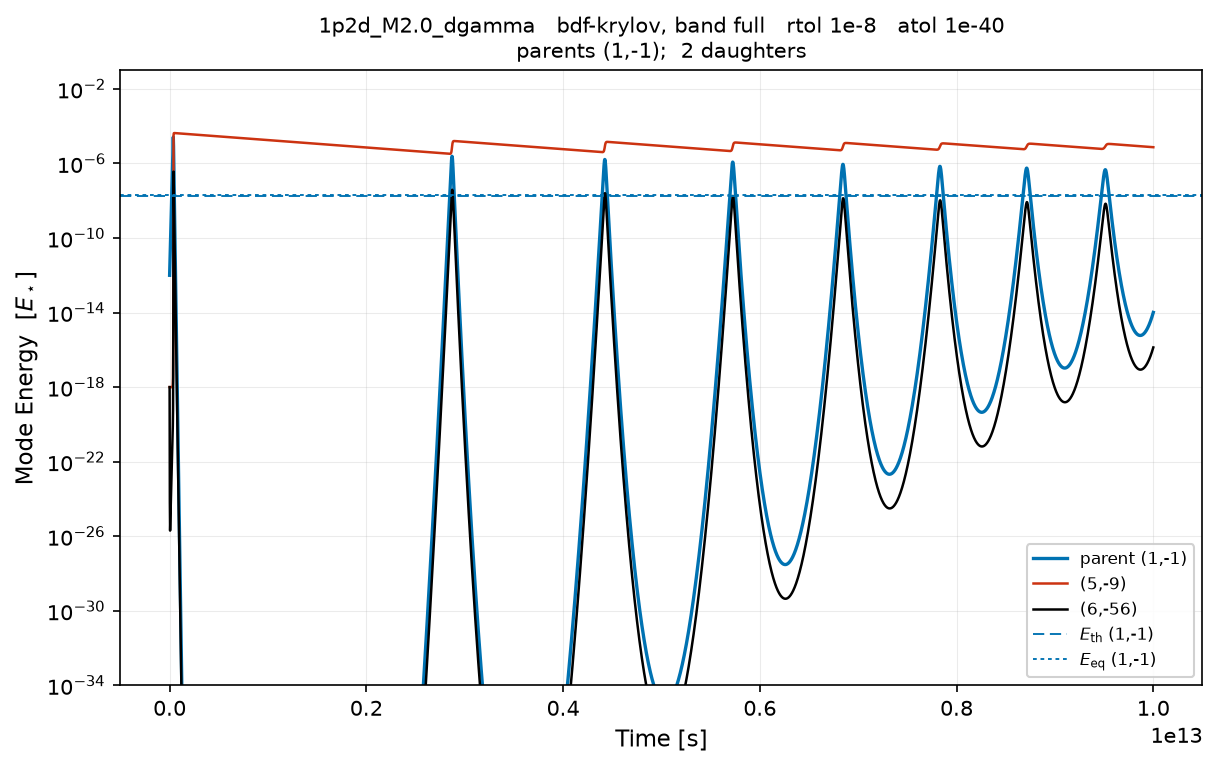
\includegraphics[width=0.21\textwidth,height=0.1323\textwidth]{../plots/krylov_full/1p2d_M2.0_dgamma/r1e-8_a1e-40.png} & 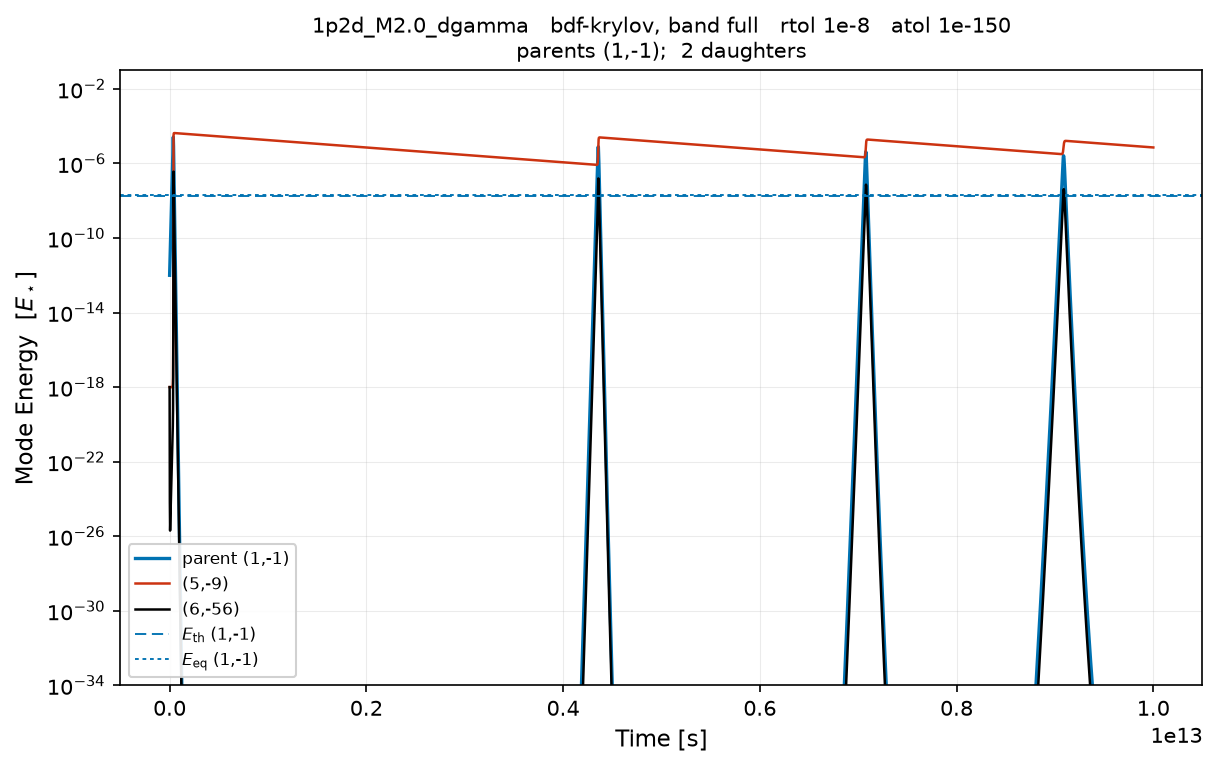
\includegraphics[width=0.21\textwidth,height=0.1323\textwidth]{../plots/krylov_full/1p2d_M2.0_dgamma/r1e-8_a1e-150.png} & 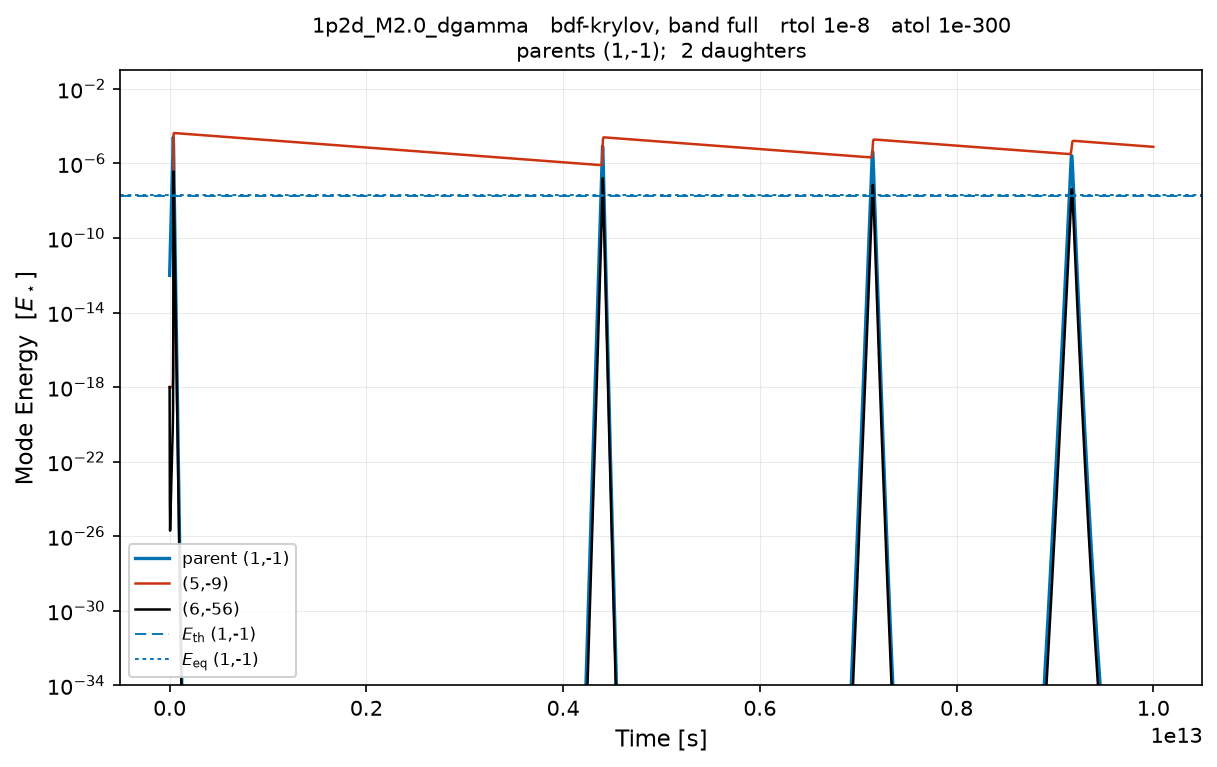
\includegraphics[width=0.21\textwidth,height=0.1323\textwidth]{../plots/krylov_full/1p2d_M2.0_dgamma/r1e-8_a1e-300.png} & 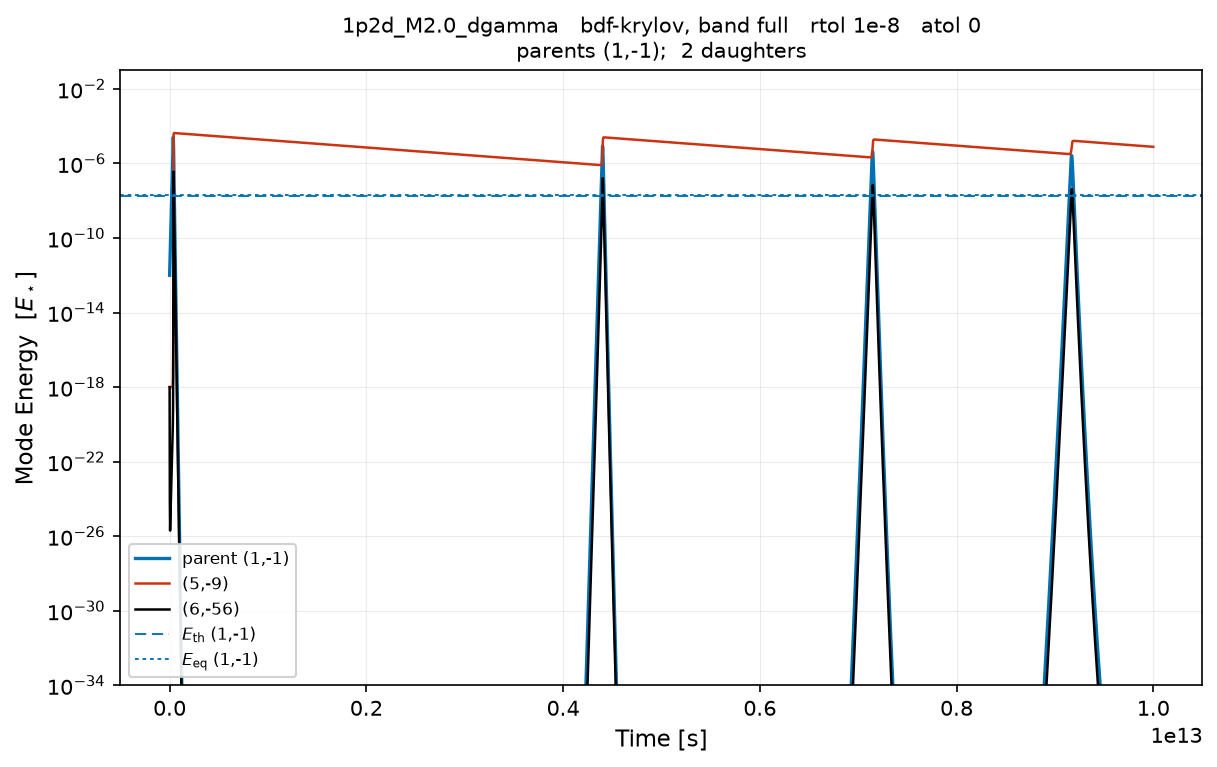
\includegraphics[width=0.21\textwidth,height=0.1323\textwidth]{../plots/krylov_full/1p2d_M2.0_dgamma/r1e-8_a0.png} \\[-1pt]
 & \parbox[t]{0.21\textwidth}{\centering\scriptsize 100.36\,M steps, 124.9\,s} & \parbox[t]{0.21\textwidth}{\centering\scriptsize 111.48\,M steps, 136.5\,s} & \parbox[t]{0.21\textwidth}{\centering\scriptsize 117.07\,M steps, 159.0\,s} & \parbox[t]{0.21\textwidth}{\centering\scriptsize 117.07\,M steps, 176.9\,s} \\[2pt]
\rotatebox{90}{\parbox{0.1323\textwidth}{\centering\scriptsize\bfseries BDF-Krylov, band 3}} & 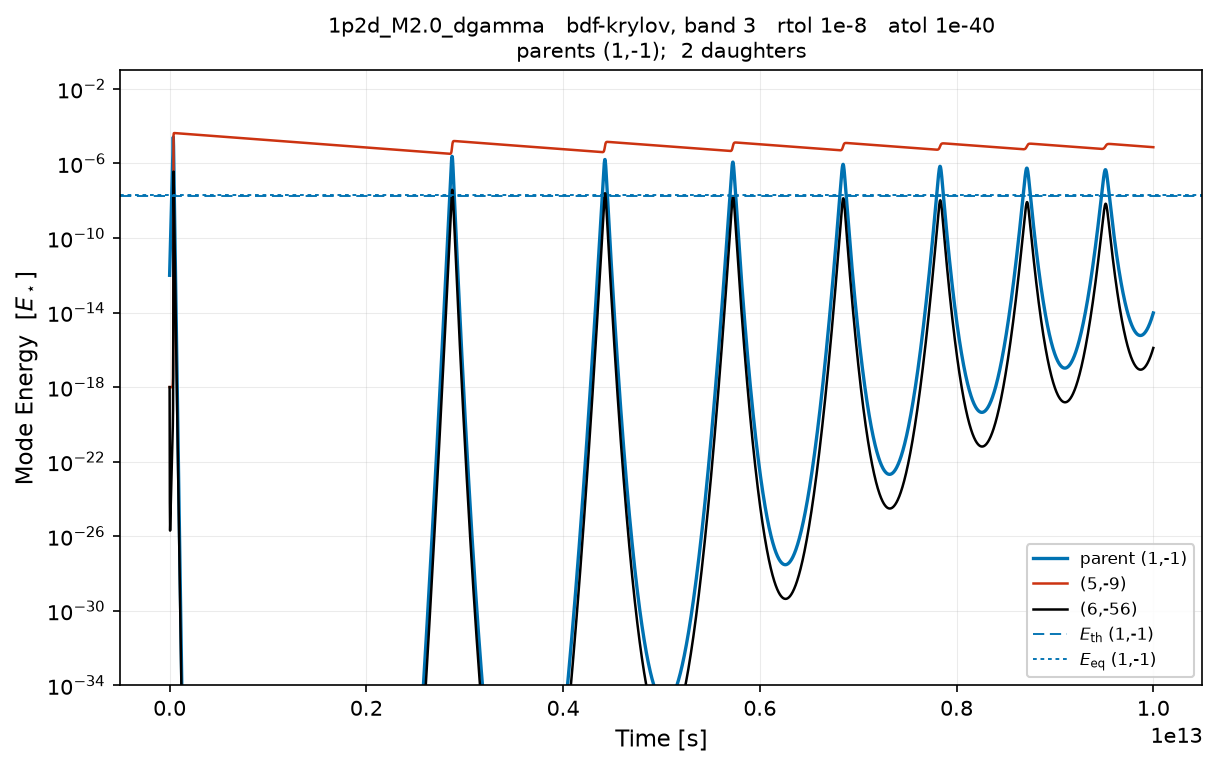
\includegraphics[width=0.21\textwidth,height=0.1323\textwidth]{../plots/krylov_b3/1p2d_M2.0_dgamma/r1e-8_a1e-40.png} & 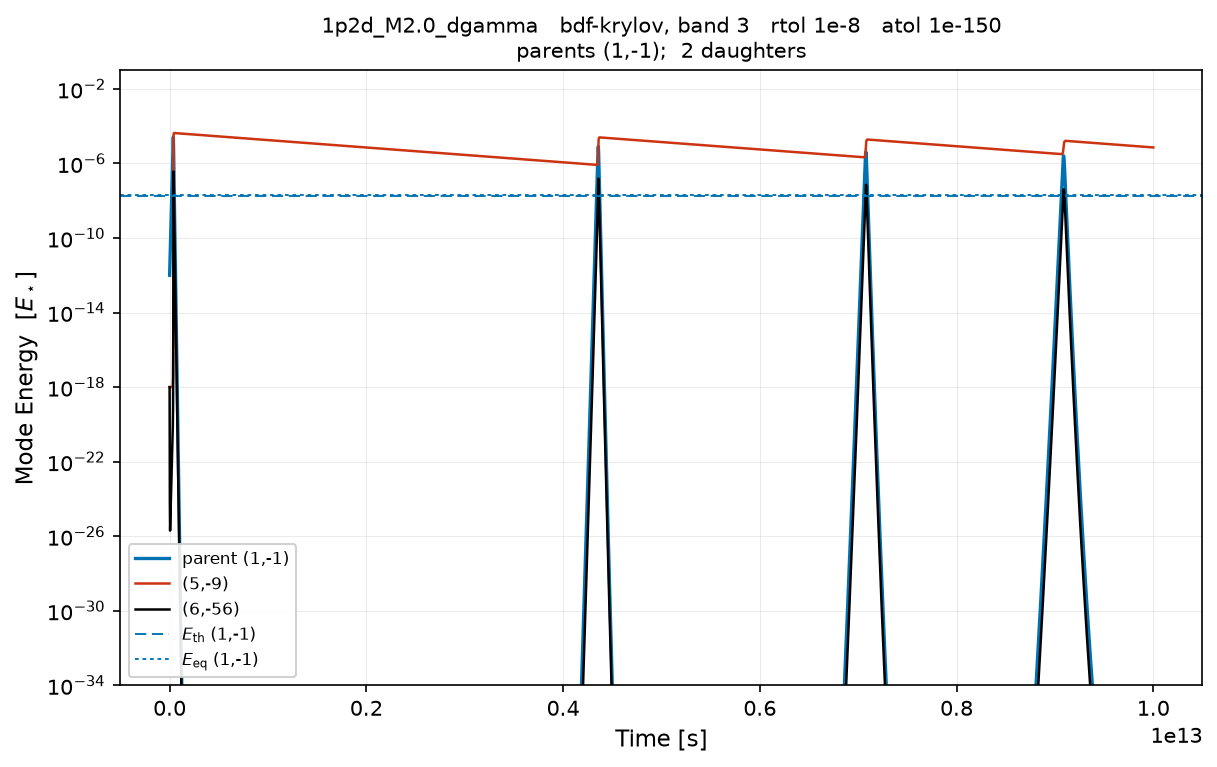
\includegraphics[width=0.21\textwidth,height=0.1323\textwidth]{../plots/krylov_b3/1p2d_M2.0_dgamma/r1e-8_a1e-150.png} & 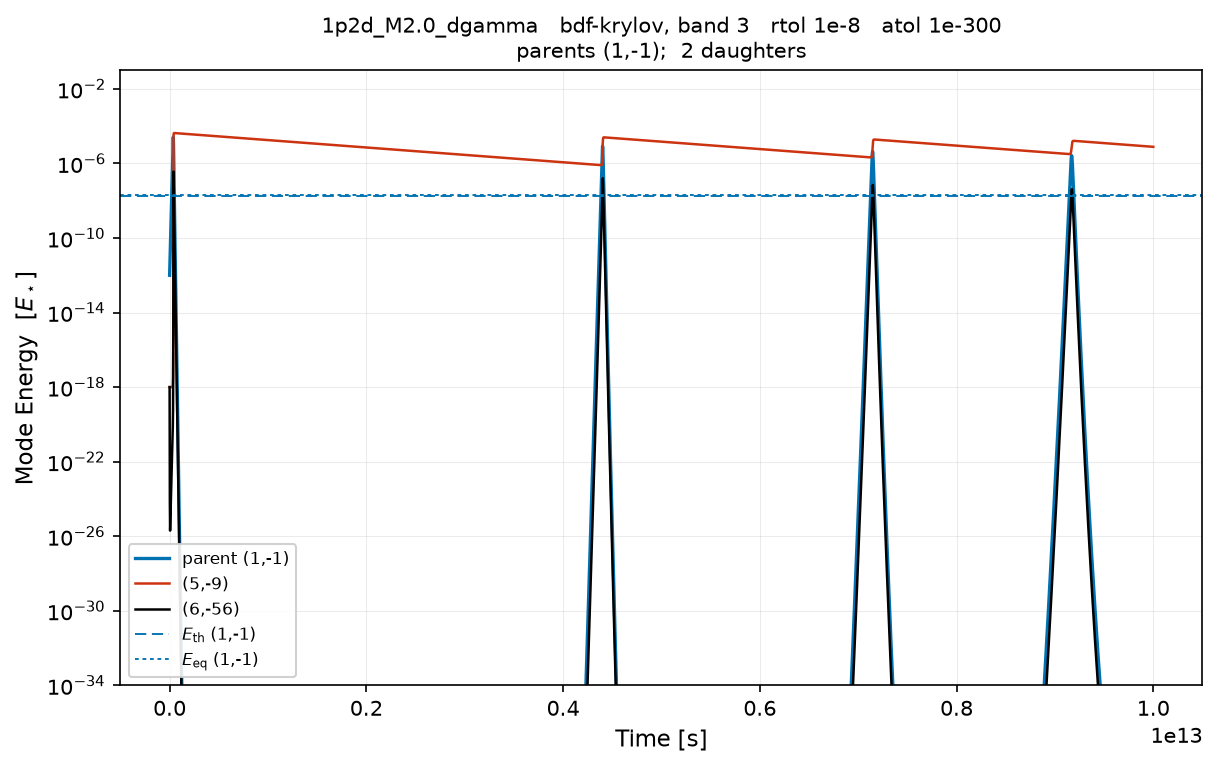
\includegraphics[width=0.21\textwidth,height=0.1323\textwidth]{../plots/krylov_b3/1p2d_M2.0_dgamma/r1e-8_a1e-300.png} & 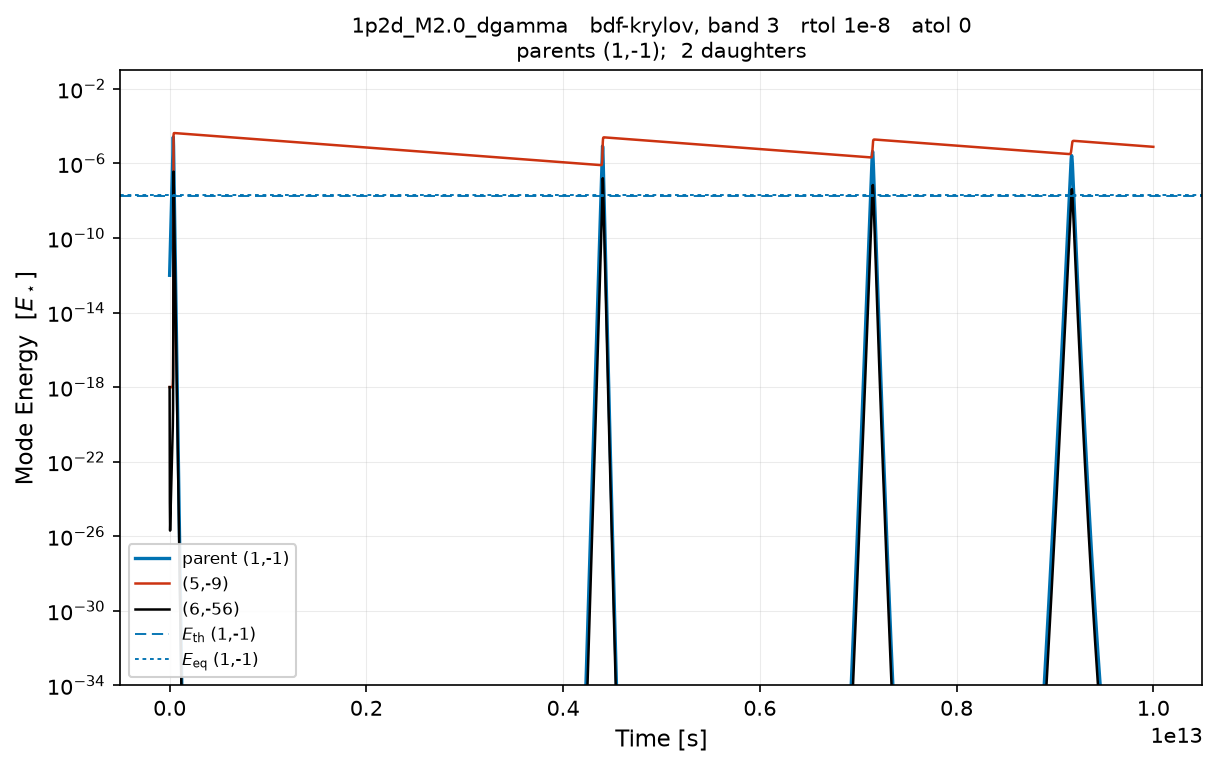
\includegraphics[width=0.21\textwidth,height=0.1323\textwidth]{../plots/krylov_b3/1p2d_M2.0_dgamma/r1e-8_a0.png} \\[-1pt]
 & \parbox[t]{0.21\textwidth}{\centering\scriptsize 99.14\,M steps, 140.6\,s} & \parbox[t]{0.21\textwidth}{\centering\scriptsize 110.16\,M steps, 156.8\,s} & \parbox[t]{0.21\textwidth}{\centering\scriptsize 115.72\,M steps, 155.0\,s} & \parbox[t]{0.21\textwidth}{\centering\scriptsize 115.72\,M steps, 204.6\,s} \\[2pt]
\rotatebox{90}{\parbox{0.1323\textwidth}{\centering\scriptsize\bfseries Adams, fixed point}} & 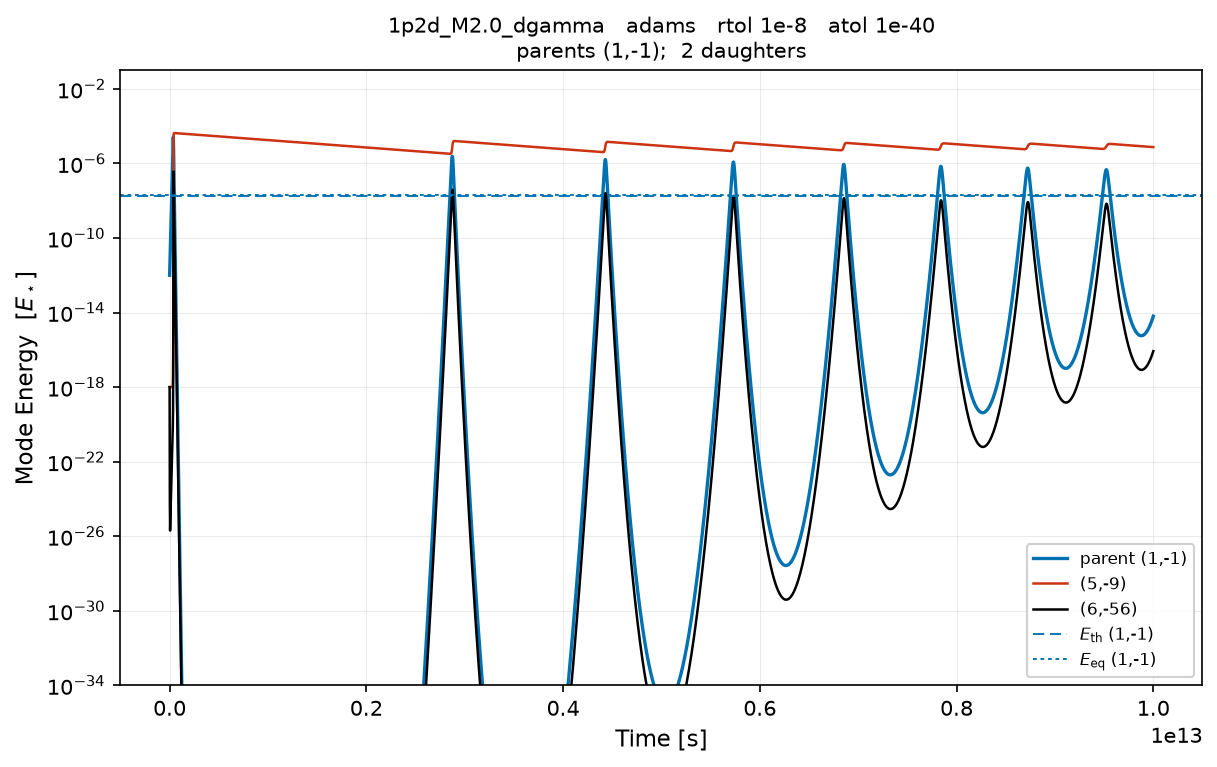
\includegraphics[width=0.21\textwidth,height=0.1323\textwidth]{../plots/adams/1p2d_M2.0_dgamma/r1e-8_a1e-40.png} & 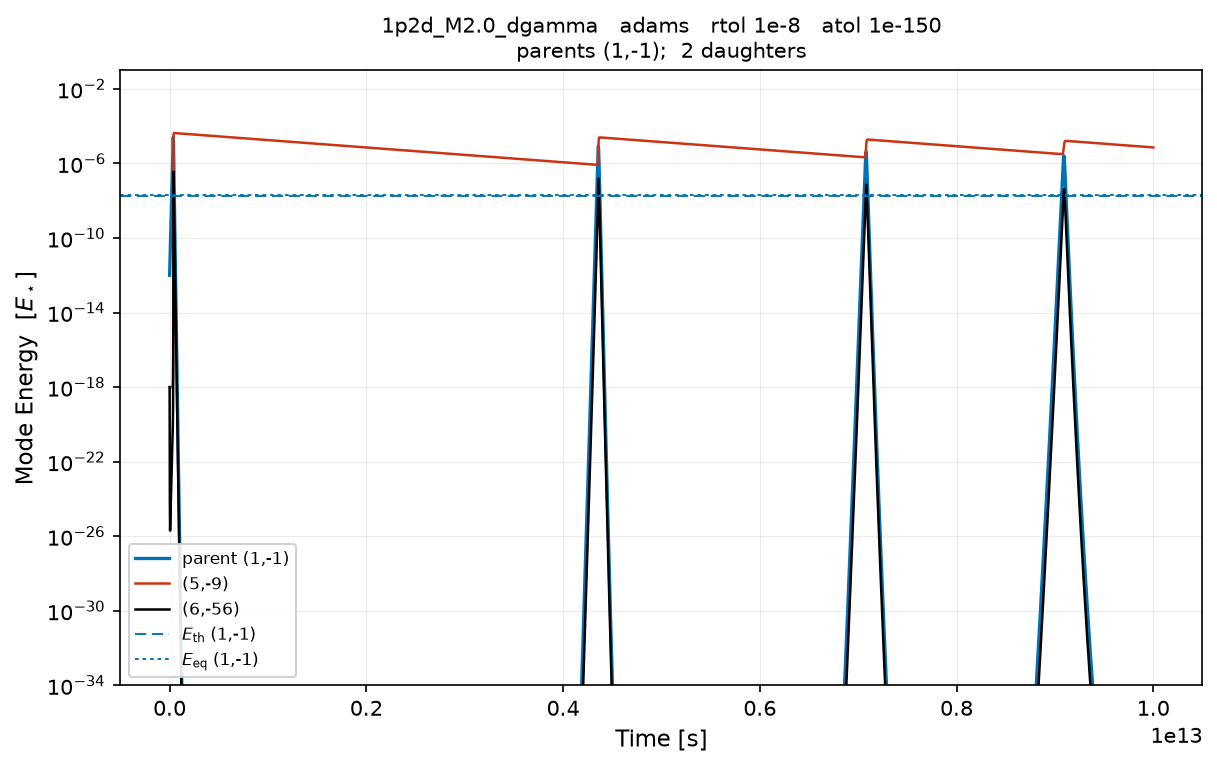
\includegraphics[width=0.21\textwidth,height=0.1323\textwidth]{../plots/adams/1p2d_M2.0_dgamma/r1e-8_a1e-150.png} & 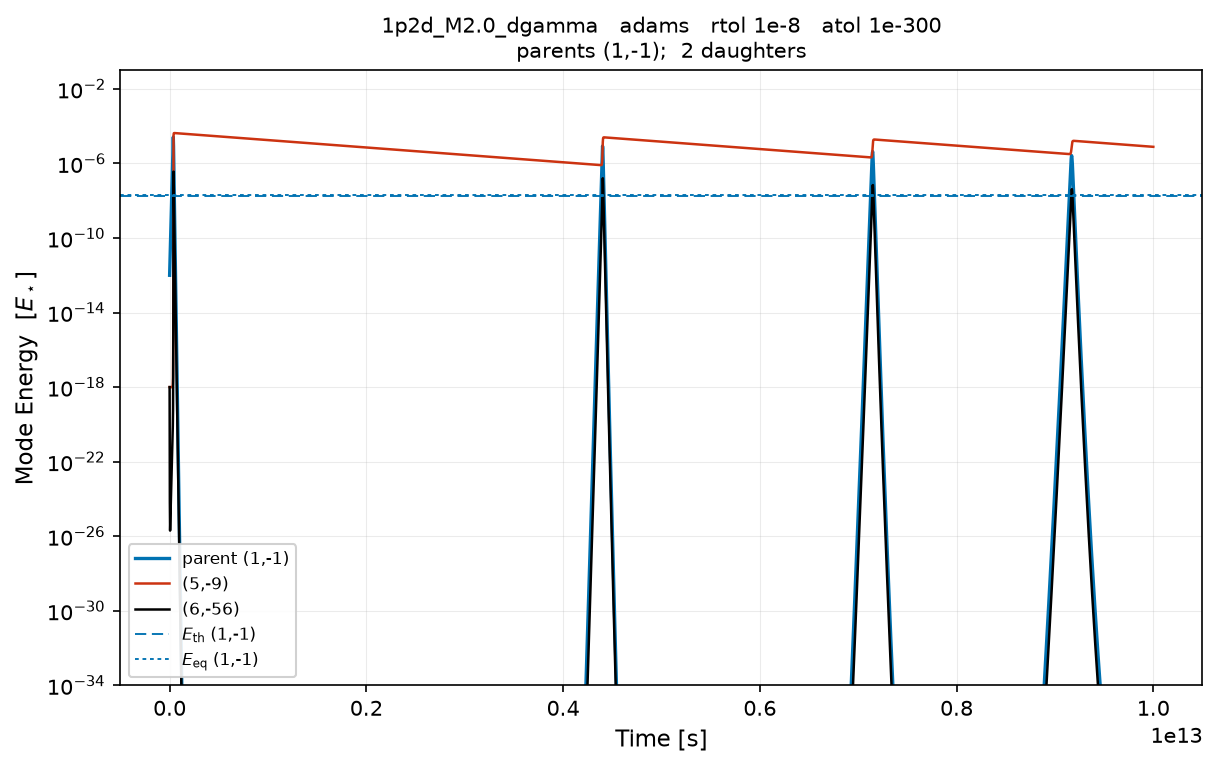
\includegraphics[width=0.21\textwidth,height=0.1323\textwidth]{../plots/adams/1p2d_M2.0_dgamma/r1e-8_a1e-300.png} & 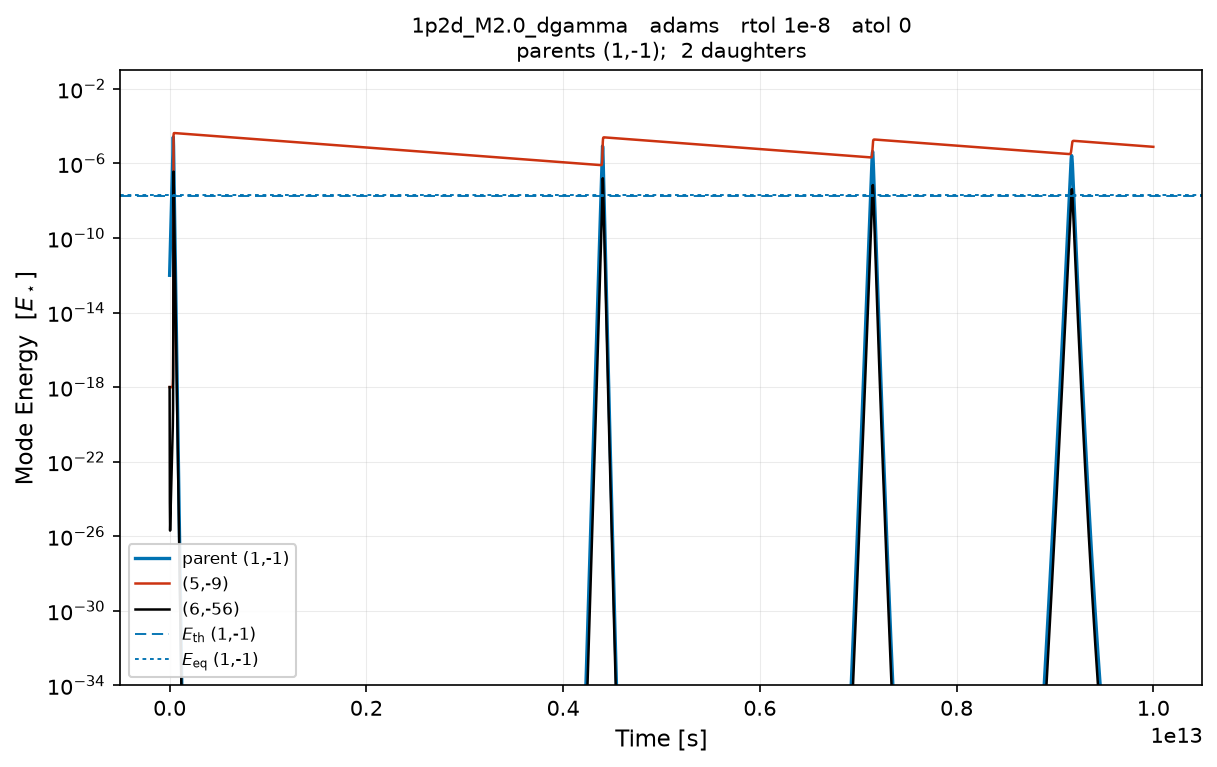
\includegraphics[width=0.21\textwidth,height=0.1323\textwidth]{../plots/adams/1p2d_M2.0_dgamma/r1e-8_a0.png} \\[-1pt]
 & \parbox[t]{0.21\textwidth}{\centering\scriptsize 43.17\,M steps, 39.5\,s} & \parbox[t]{0.21\textwidth}{\centering\scriptsize 47.54\,M steps, 45.3\,s} & \parbox[t]{0.21\textwidth}{\centering\scriptsize 48.28\,M steps, 54.4\,s} & \parbox[t]{0.21\textwidth}{\centering\scriptsize 48.28\,M steps, 43.5\,s} \\[2pt]
\end{tabular}\par}
\par\noindent{\scriptsize\setlength\tabcolsep{3.5pt}\renewcommand\arraystretch{0.92}
\begin{tabular}{@{}llllrrrrrrr@{}}
\toprule
integrator & atol & stop & $t_{\rm stop}$ [s] & steps & rejected & RHS & Jac. & NL it. & lin. it. & wall [s] \\
\midrule
rk8pd & $10^{-40}$ & end & $1.00\times10^{13}$ & 6.61\,M & 575.7\,k & 85.89\,M & -- & -- & -- & 9.5 \\
 & $10^{-150}$ & end & $1.00\times10^{13}$ & 8.24\,M & 937.9\,k & 107.11\,M & -- & -- & -- & 15.6 \\
 & $10^{-300}$ & end & $1.00\times10^{13}$ & 9.26\,M & 1.04\,M & 120.43\,M & -- & -- & -- & 13.5 \\
 & $0$ & end & $1.00\times10^{13}$ & 9.26\,M & 1.04\,M & 120.43\,M & -- & -- & -- & 20.4 \\
\addlinespace[2pt]
BDF, dense analytic Jacobian & $10^{-40}$ & end & $1.00\times10^{13}$ & 14.40\,M & 215.6\,k & 16.26\,M & 378.7\,k & 16.26\,M & -- & 12.8 \\
 & $10^{-150}$ & end & $1.00\times10^{13}$ & 114.97\,M & 655.1\,k & 121.60\,M & 1.93\,M & 121.59\,M & -- & 154.3 \\
 & $10^{-300}$ & end & $1.00\times10^{13}$ & 120.93\,M & 719.2\,k & 127.92\,M & 2.03\,M & 127.91\,M & -- & 140.1 \\
 & $0$ & end & $1.00\times10^{13}$ & 120.93\,M & 719.2\,k & 127.92\,M & 2.03\,M & 127.91\,M & -- & 168.2 \\
\addlinespace[2pt]
BDF-Krylov, band full & $10^{-40}$ & end & $1.00\times10^{13}$ & 100.36\,M & 648.8\,k & 225.12\,M & 1.69\,M & 107.09\,M & 107.90\,M & 124.9 \\
 & $10^{-150}$ & end & $1.00\times10^{13}$ & 111.48\,M & 738.1\,k & 246.46\,M & 1.87\,M & 118.93\,M & 116.29\,M & 136.5 \\
 & $10^{-300}$ & end & $1.00\times10^{13}$ & 117.07\,M & 821.6\,k & 257.00\,M & 1.97\,M & 124.94\,M & 120.27\,M & 159.0 \\
 & $0$ & end & $1.00\times10^{13}$ & 117.07\,M & 821.6\,k & 257.00\,M & 1.97\,M & 124.94\,M & 120.27\,M & 176.9 \\
\addlinespace[2pt]
BDF-Krylov, band 3 & $10^{-40}$ & end & $1.00\times10^{13}$ & 99.14\,M & 679.3\,k & 223.80\,M & 1.66\,M & 106.16\,M & 107.65\,M & 140.6 \\
 & $10^{-150}$ & end & $1.00\times10^{13}$ & 110.16\,M & 777.2\,k & 244.85\,M & 1.85\,M & 117.94\,M & 115.81\,M & 156.8 \\
 & $10^{-300}$ & end & $1.00\times10^{13}$ & 115.72\,M & 853.2\,k & 255.64\,M & 1.94\,M & 123.92\,M & 120.06\,M & 155.0 \\
 & $0$ & end & $1.00\times10^{13}$ & 115.72\,M & 853.2\,k & 255.64\,M & 1.94\,M & 123.92\,M & 120.06\,M & 204.6 \\
\addlinespace[2pt]
Adams, fixed point & $10^{-40}$ & end & $1.00\times10^{13}$ & 43.17\,M & 1.65\,M & 61.88\,M & -- & 61.88\,M & -- & 39.5 \\
 & $10^{-150}$ & end & $1.00\times10^{13}$ & 47.54\,M & 2.13\,M & 69.35\,M & -- & 69.35\,M & -- & 45.3 \\
 & $10^{-300}$ & end & $1.00\times10^{13}$ & 48.28\,M & 2.32\,M & 68.68\,M & -- & 68.68\,M & -- & 54.4 \\
 & $0$ & end & $1.00\times10^{13}$ & 48.28\,M & 2.32\,M & 68.68\,M & -- & 68.68\,M & -- & 43.5 \\
\bottomrule
\end{tabular}}

\clearpage
\subsection{\texttt{1p4d\_M1.7\_eth}}\label{net:1p4d_M1.7_eth}
\noindent\begin{minipage}[t]{0.43\textwidth}\vspace{0pt}\footnotesize
\begin{tabular}{@{}rrlrr@{}}
\toprule
id & gen & $(\ell,n)$ & $\omega$ [rad\,s$^{-1}$] & $\gamma$ [s$^{-1}$] \\
\midrule
0 & 0 & (1,+1) & $1.402\times10^{-3}$ & $-1.150\times10^{-10}$ \\
1 & 1 & (6,$-$6) & $1.070\times10^{-3}$ & $4.184\times10^{-13}$ \\
2 & 1 & (7,$-$27) & $3.326\times10^{-4}$ & $8.612\times10^{-10}$ \\
3 & 1 & (5,$-$14) & $4.541\times10^{-4}$ & $7.998\times10^{-12}$ \\
4 & 1 & (6,$-$7) & $9.483\times10^{-4}$ & $7.855\times10^{-13}$ \\
\bottomrule
\end{tabular}
\end{minipage}\hfill
\begin{minipage}[t]{0.55\textwidth}\vspace{0pt}\footnotesize
\textbf{Model} \texttt{dsct\_M1.7\_T7750}, rule eth, $N=4$, cut 0.15,
closure 0.005; 5 modes, 2 triplet(s).\\[2pt]
\textbf{Selecting pairs}\\ (1,+1) $\to$ (6,$-$6) + (7,$-$27): $\Delta/\omega_a=-3.98\times10^{-5}$, $\kappa=+0.107$, $E_{\rm th}=9.22\times10^{-11}$, $E_{\rm eq}=1.23\times10^{-10}$\\
(1,+1) $\to$ (5,$-$14) + (6,$-$7): $\Delta/\omega_a=1.51\times10^{-5}$, $\kappa=+0.369$, $E_{\rm th}=1.57\times10^{-10}$, no $E_{\rm eq}$\\[2pt]
Runaway near $3\times10^{11}$\,s.
\end{minipage}

\par\smallskip{\centering\begin{tabular}{@{}c@{\hspace{2pt}}c@{\hspace{2pt}}c@{\hspace{2pt}}c@{\hspace{2pt}}c@{}}
 & \small atol $10^{-40}$ & \small atol $10^{-150}$ & \small atol $10^{-300}$ & \small atol $0$ \\[1pt]
\rotatebox{90}{\parbox{0.1323\textwidth}{\centering\scriptsize\bfseries rk8pd}} & 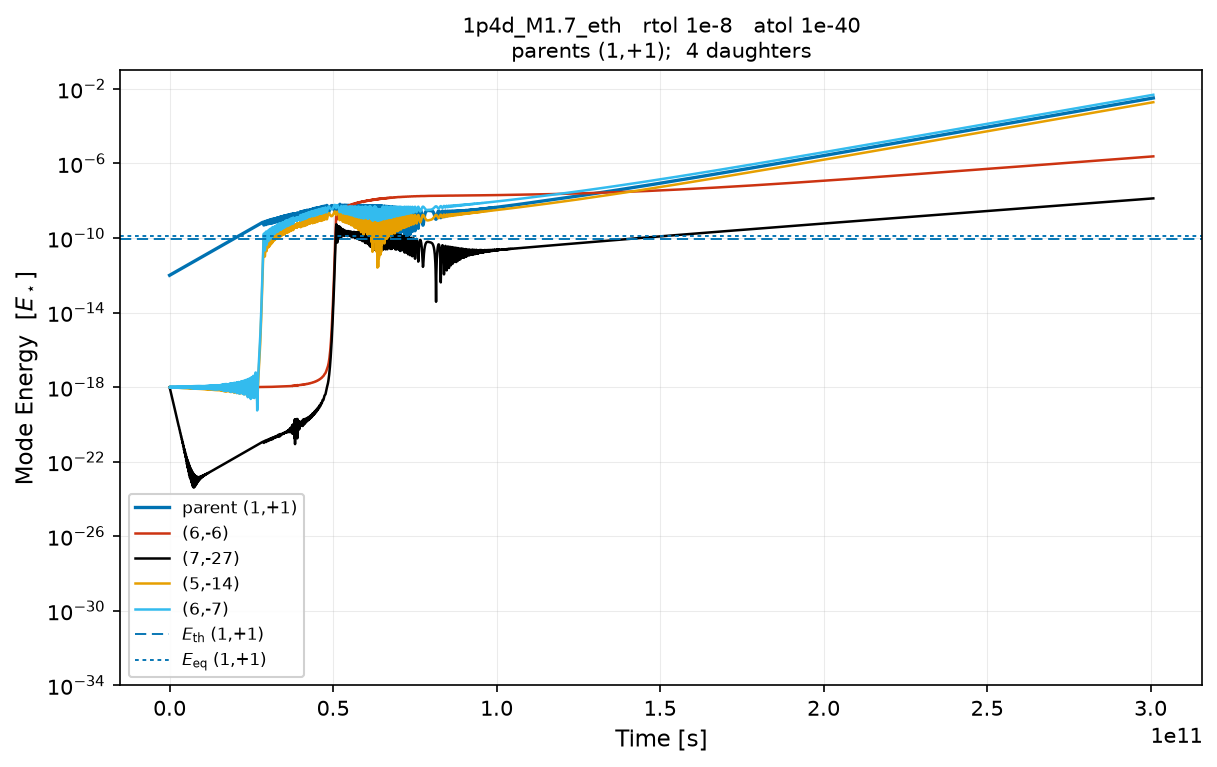
\includegraphics[width=0.21\textwidth,height=0.1323\textwidth]{../plots/rk8pd/1p4d_M1.7_eth/r1e-8_a1e-40.png} & 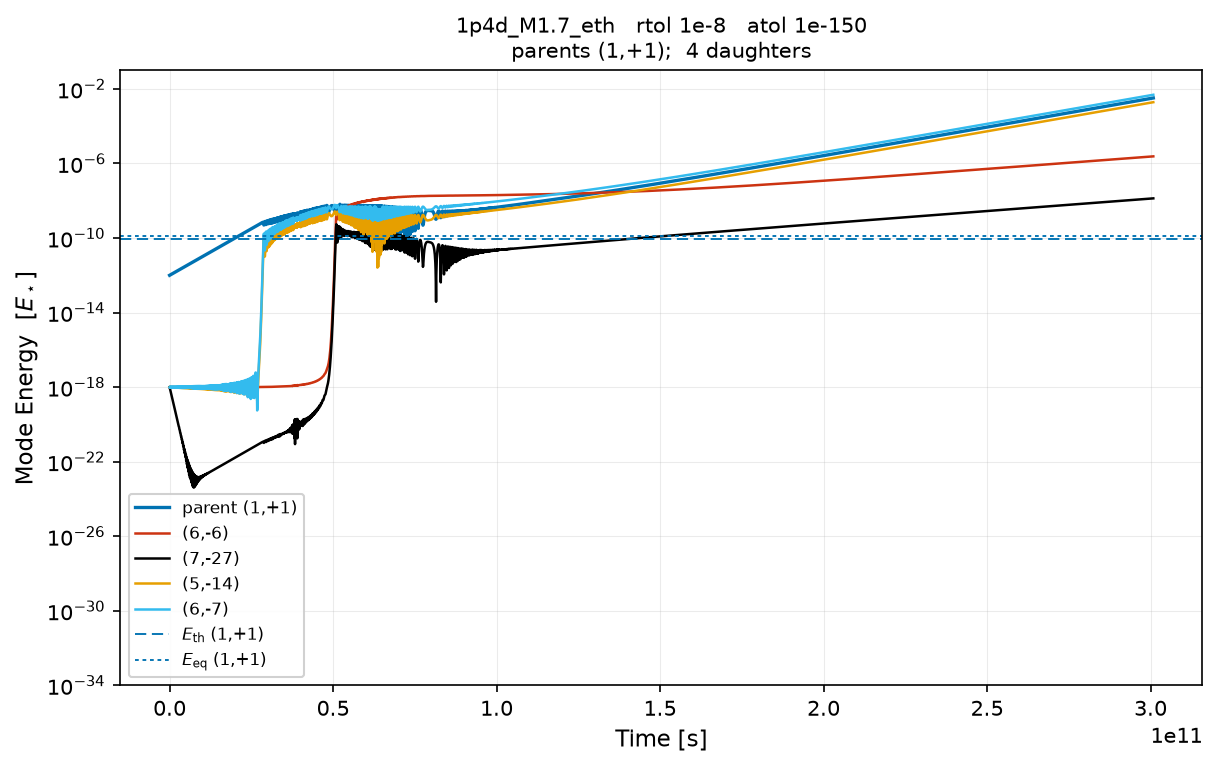
\includegraphics[width=0.21\textwidth,height=0.1323\textwidth]{../plots/rk8pd/1p4d_M1.7_eth/r1e-8_a1e-150.png} & 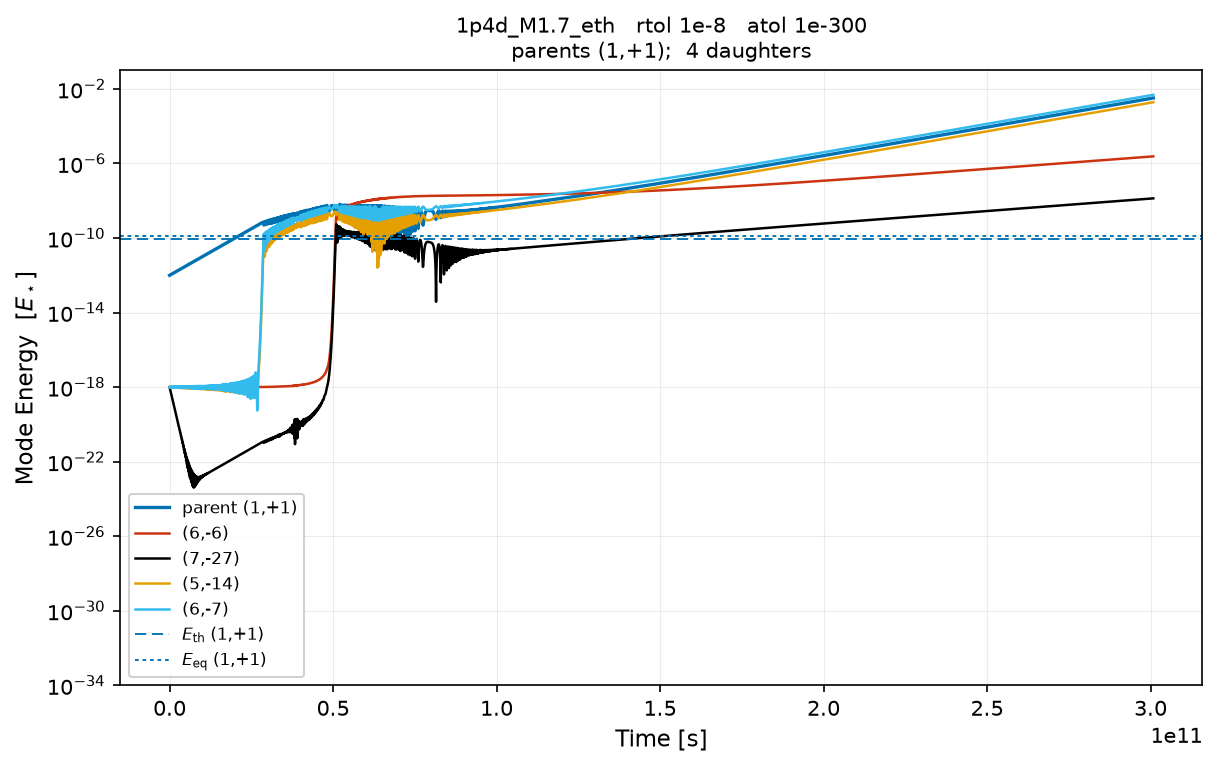
\includegraphics[width=0.21\textwidth,height=0.1323\textwidth]{../plots/rk8pd/1p4d_M1.7_eth/r1e-8_a1e-300.png} & 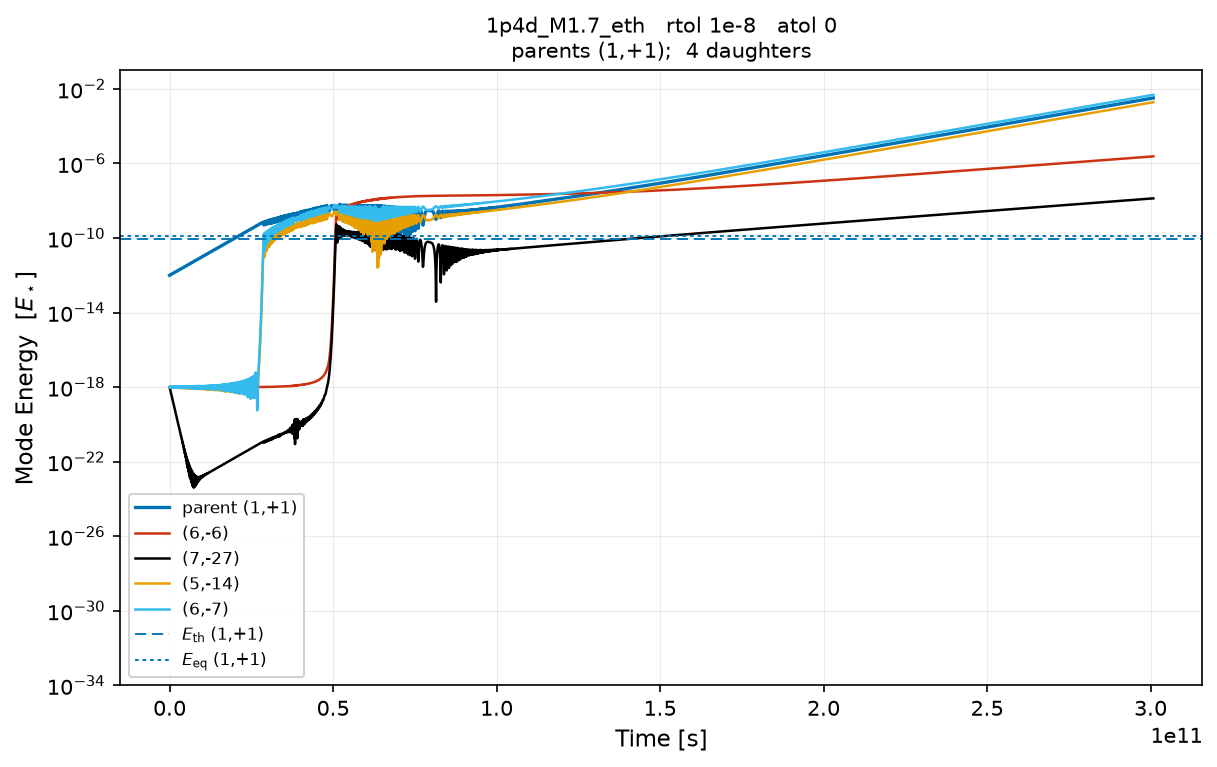
\includegraphics[width=0.21\textwidth,height=0.1323\textwidth]{../plots/rk8pd/1p4d_M1.7_eth/r1e-8_a0.png} \\[-1pt]
 & \parbox[t]{0.21\textwidth}{\centering\scriptsize 7.58\,M steps, 19.8\,s, runaway} & \parbox[t]{0.21\textwidth}{\centering\scriptsize 7.58\,M steps, 17.7\,s, runaway} & \parbox[t]{0.21\textwidth}{\centering\scriptsize 7.58\,M steps, 18.4\,s, runaway} & \parbox[t]{0.21\textwidth}{\centering\scriptsize 7.58\,M steps, 19.8\,s, runaway} \\[2pt]
\rotatebox{90}{\parbox{0.1323\textwidth}{\centering\scriptsize\bfseries BDF, dense analytic Jacobian}} & 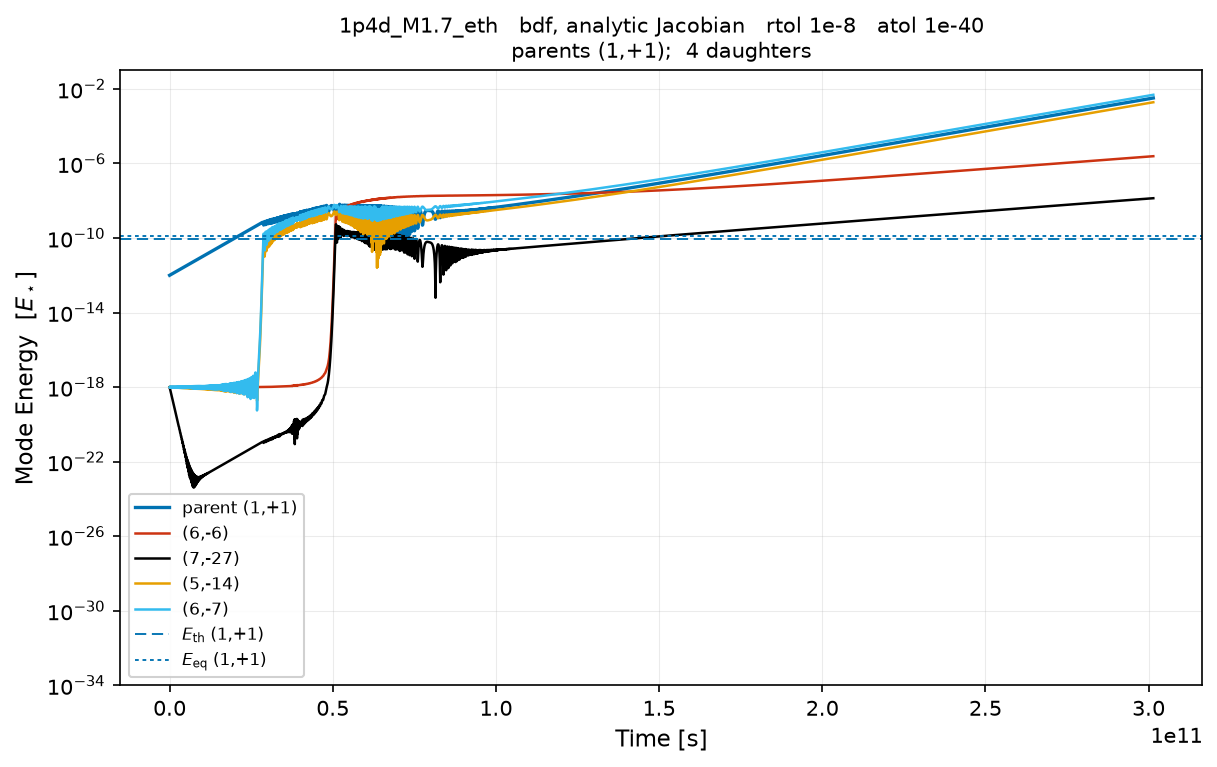
\includegraphics[width=0.21\textwidth,height=0.1323\textwidth]{../plots/bdf/1p4d_M1.7_eth/r1e-8_a1e-40.png} & 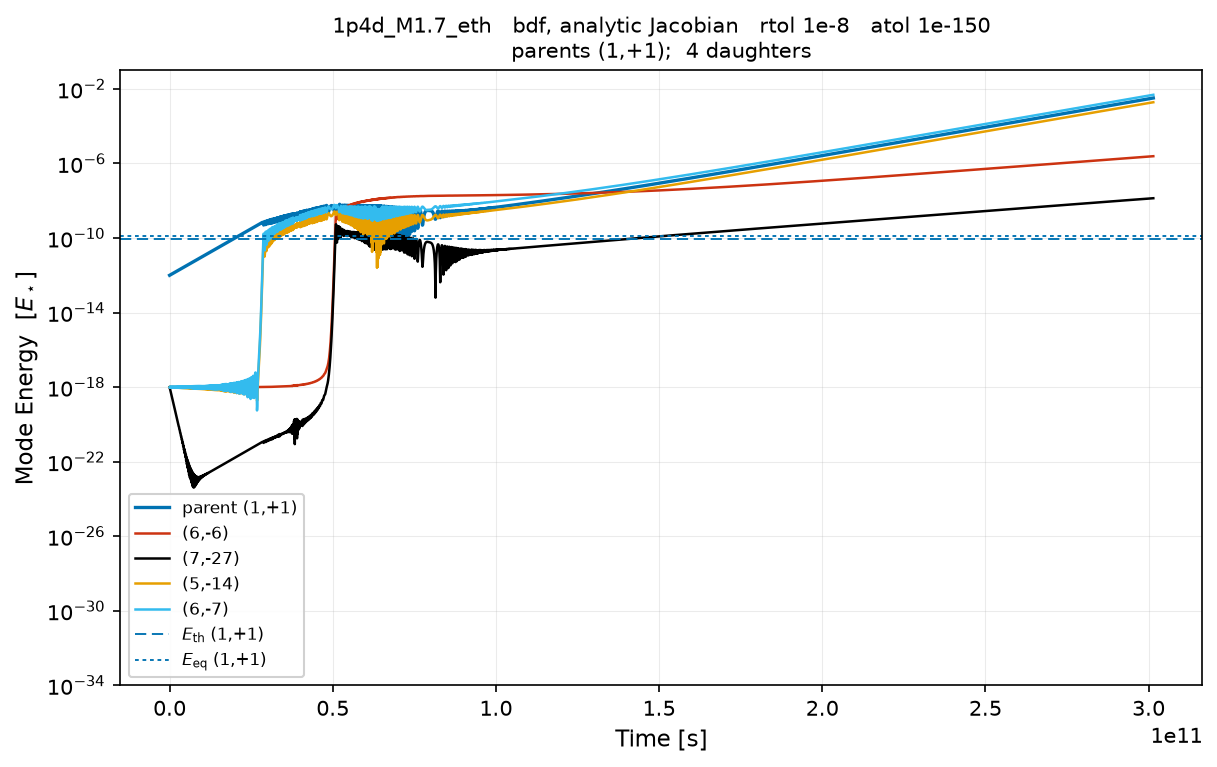
\includegraphics[width=0.21\textwidth,height=0.1323\textwidth]{../plots/bdf/1p4d_M1.7_eth/r1e-8_a1e-150.png} & 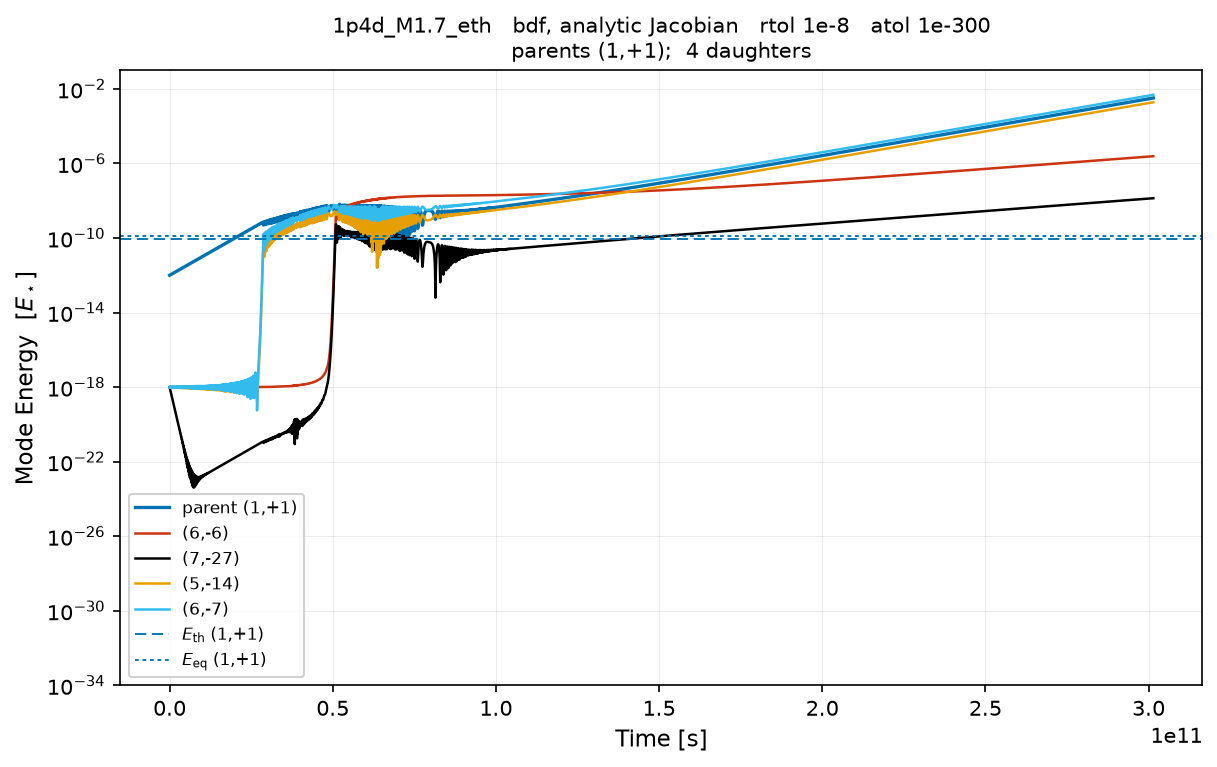
\includegraphics[width=0.21\textwidth,height=0.1323\textwidth]{../plots/bdf/1p4d_M1.7_eth/r1e-8_a1e-300.png} & 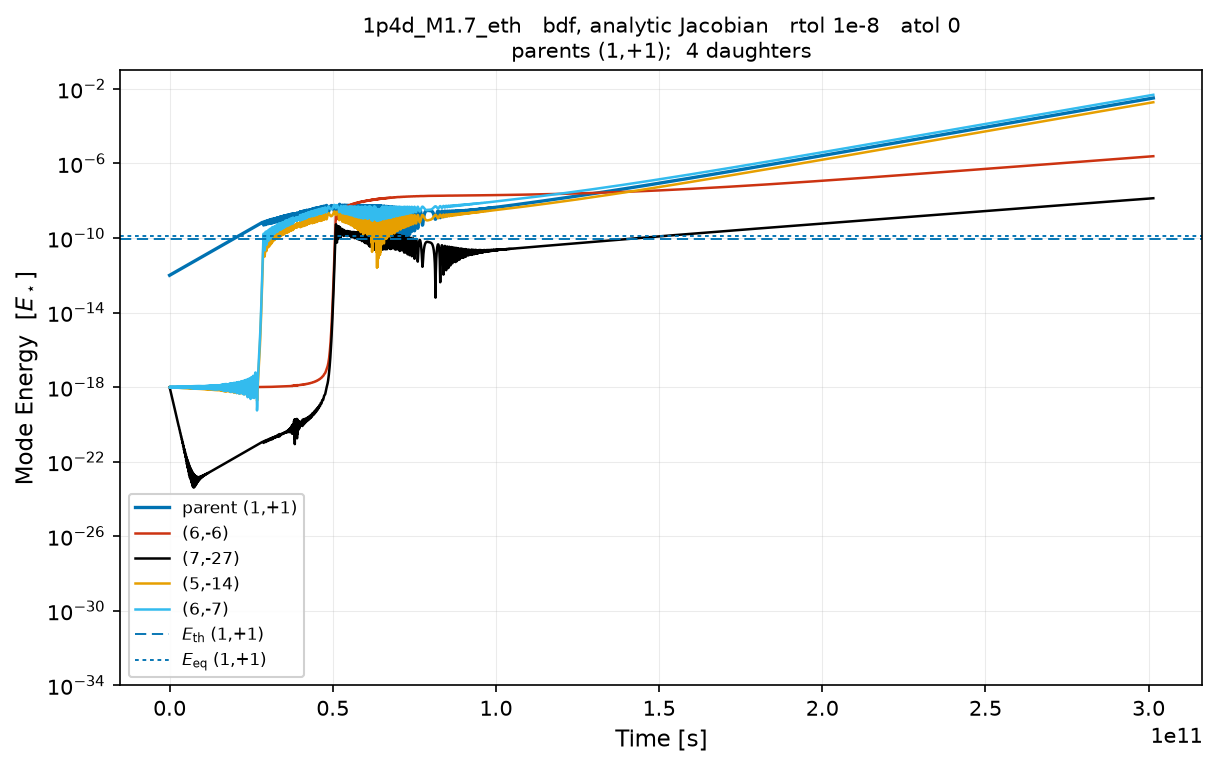
\includegraphics[width=0.21\textwidth,height=0.1323\textwidth]{../plots/bdf/1p4d_M1.7_eth/r1e-8_a0.png} \\[-1pt]
 & \parbox[t]{0.21\textwidth}{\centering\scriptsize 72.42\,M steps, 74.9\,s, runaway} & \parbox[t]{0.21\textwidth}{\centering\scriptsize 72.41\,M steps, 74.4\,s, runaway} & \parbox[t]{0.21\textwidth}{\centering\scriptsize 72.41\,M steps, 122.1\,s, runaway} & \parbox[t]{0.21\textwidth}{\centering\scriptsize 72.41\,M steps, 90.0\,s, runaway} \\[2pt]
\rotatebox{90}{\parbox{0.1323\textwidth}{\centering\scriptsize\bfseries BDF-Krylov, band full}} & 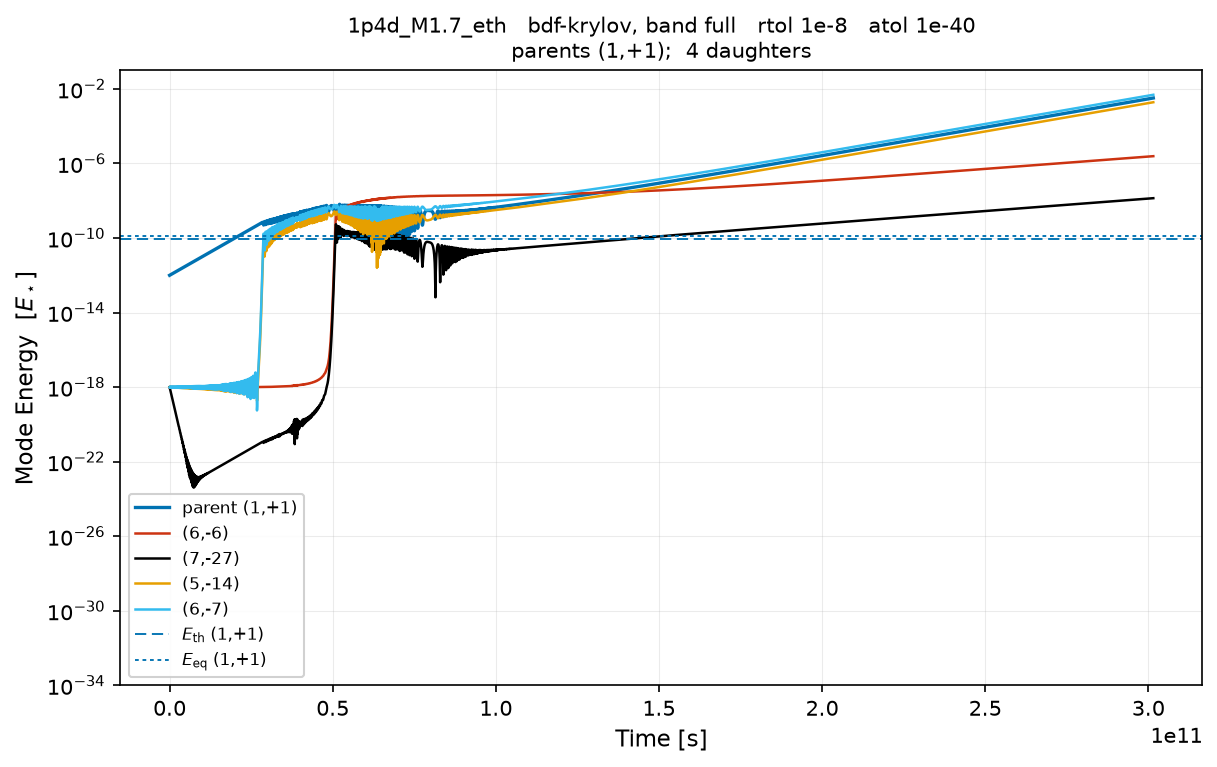
\includegraphics[width=0.21\textwidth,height=0.1323\textwidth]{../plots/krylov_full/1p4d_M1.7_eth/r1e-8_a1e-40.png} & 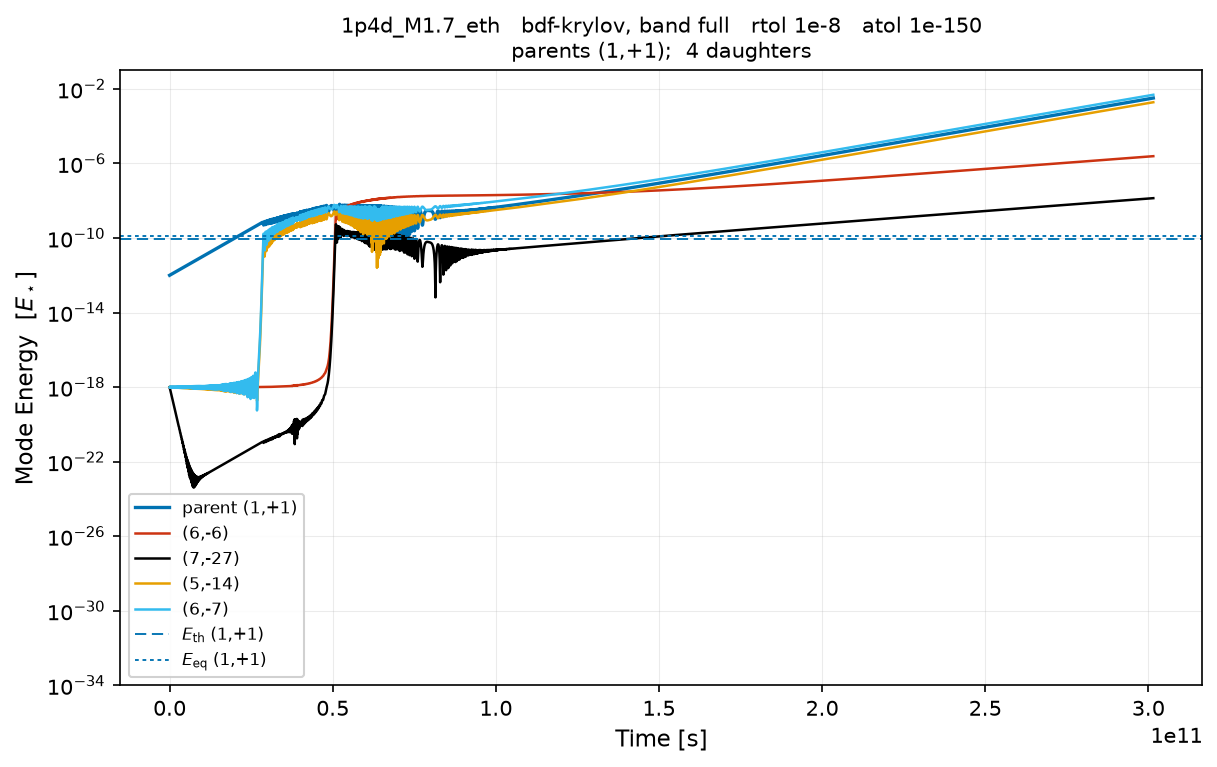
\includegraphics[width=0.21\textwidth,height=0.1323\textwidth]{../plots/krylov_full/1p4d_M1.7_eth/r1e-8_a1e-150.png} & 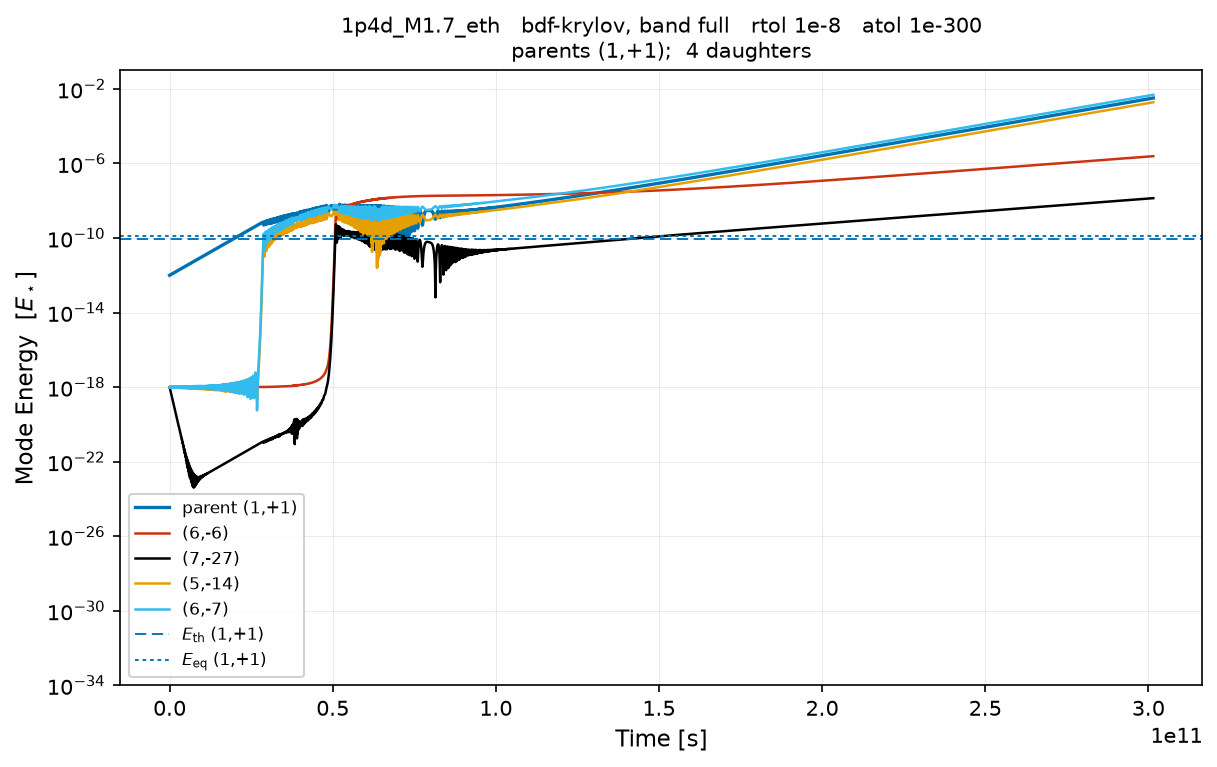
\includegraphics[width=0.21\textwidth,height=0.1323\textwidth]{../plots/krylov_full/1p4d_M1.7_eth/r1e-8_a1e-300.png} & 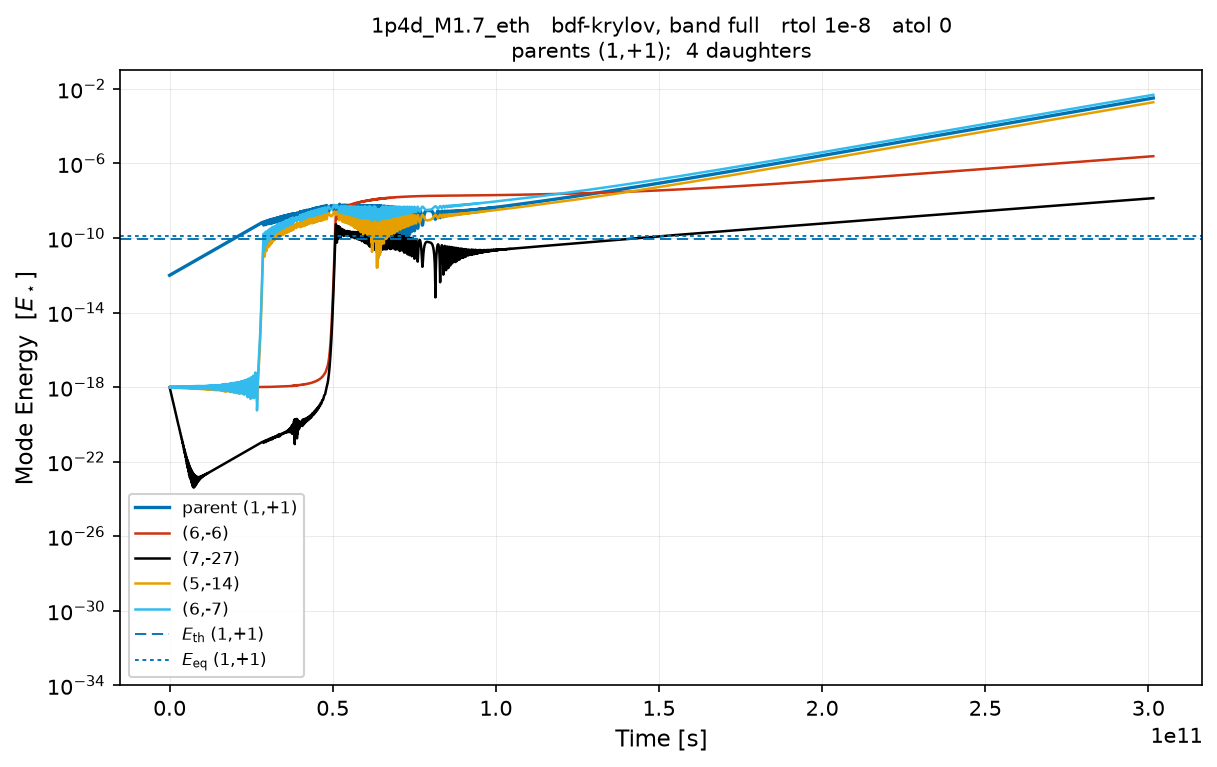
\includegraphics[width=0.21\textwidth,height=0.1323\textwidth]{../plots/krylov_full/1p4d_M1.7_eth/r1e-8_a0.png} \\[-1pt]
 & \parbox[t]{0.21\textwidth}{\centering\scriptsize 69.74\,M steps, 133.2\,s, runaway} & \parbox[t]{0.21\textwidth}{\centering\scriptsize 69.63\,M steps, 134.7\,s, runaway} & \parbox[t]{0.21\textwidth}{\centering\scriptsize 69.63\,M steps, 109.1\,s, runaway} & \parbox[t]{0.21\textwidth}{\centering\scriptsize 69.63\,M steps, 117.5\,s, runaway} \\[2pt]
\rotatebox{90}{\parbox{0.1323\textwidth}{\centering\scriptsize\bfseries BDF-Krylov, band 3}} & 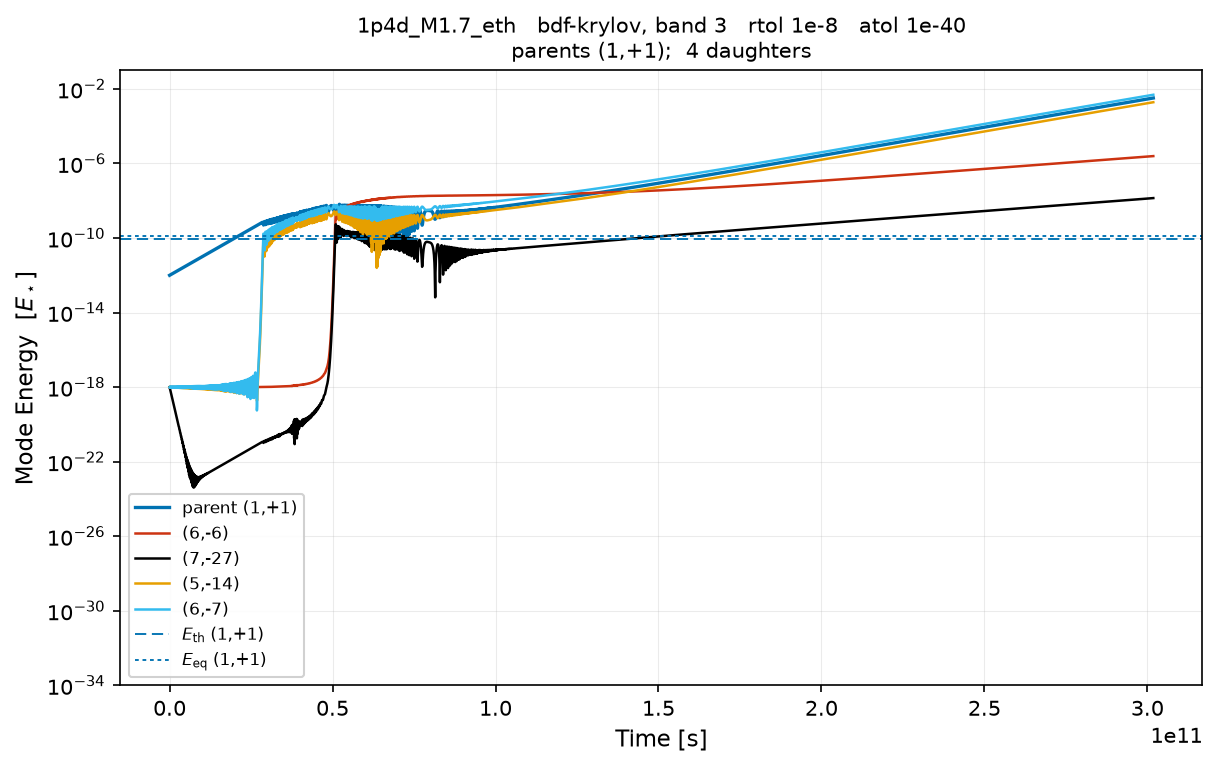
\includegraphics[width=0.21\textwidth,height=0.1323\textwidth]{../plots/krylov_b3/1p4d_M1.7_eth/r1e-8_a1e-40.png} & 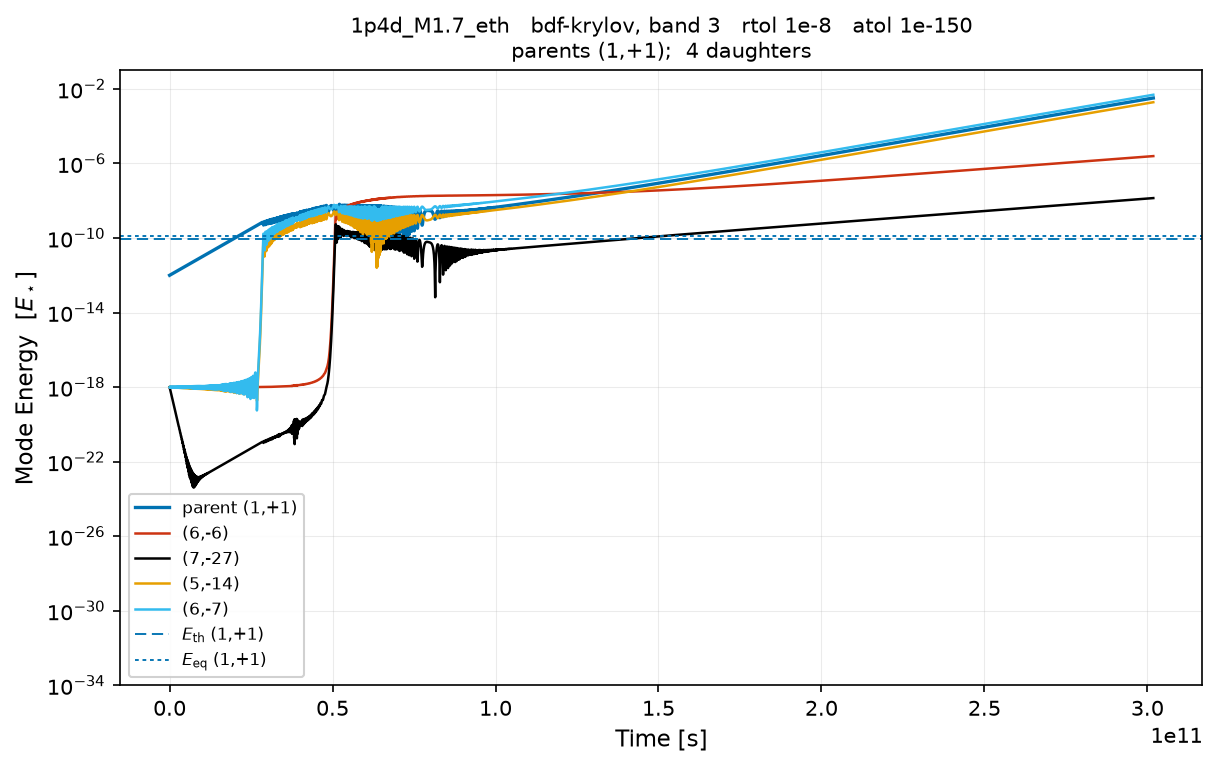
\includegraphics[width=0.21\textwidth,height=0.1323\textwidth]{../plots/krylov_b3/1p4d_M1.7_eth/r1e-8_a1e-150.png} & 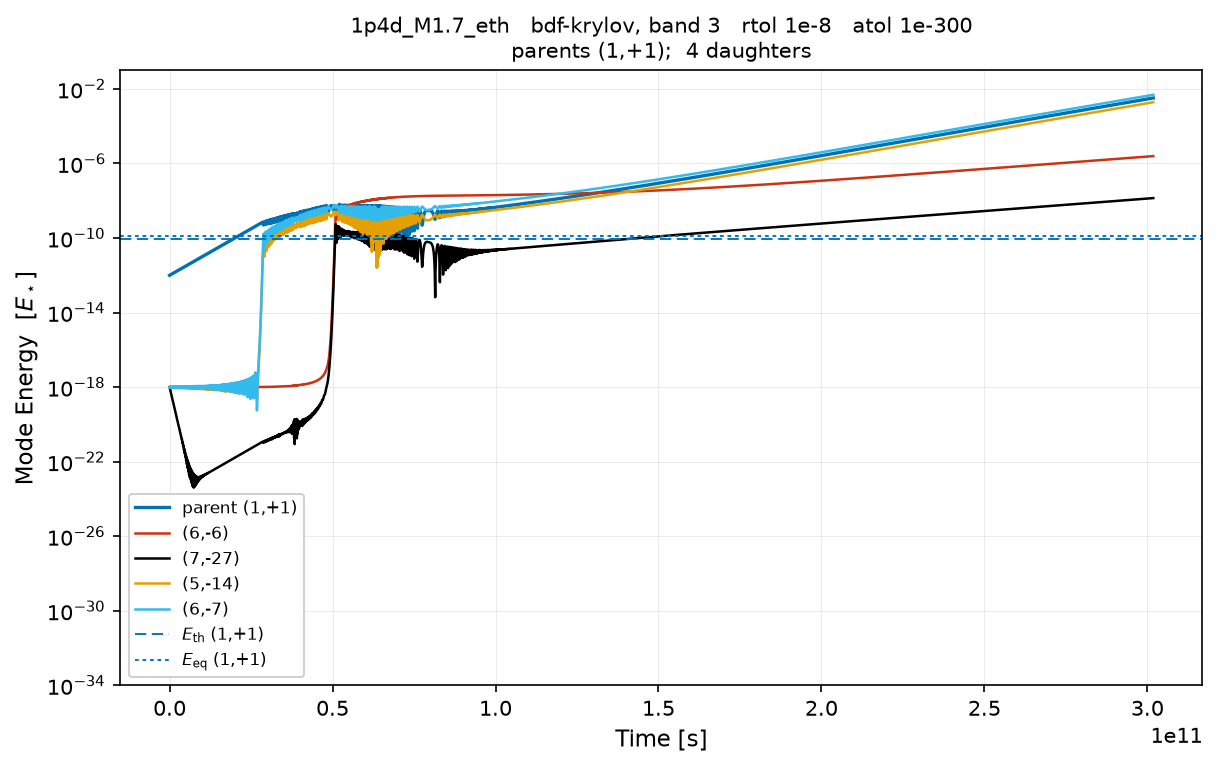
\includegraphics[width=0.21\textwidth,height=0.1323\textwidth]{../plots/krylov_b3/1p4d_M1.7_eth/r1e-8_a1e-300.png} & 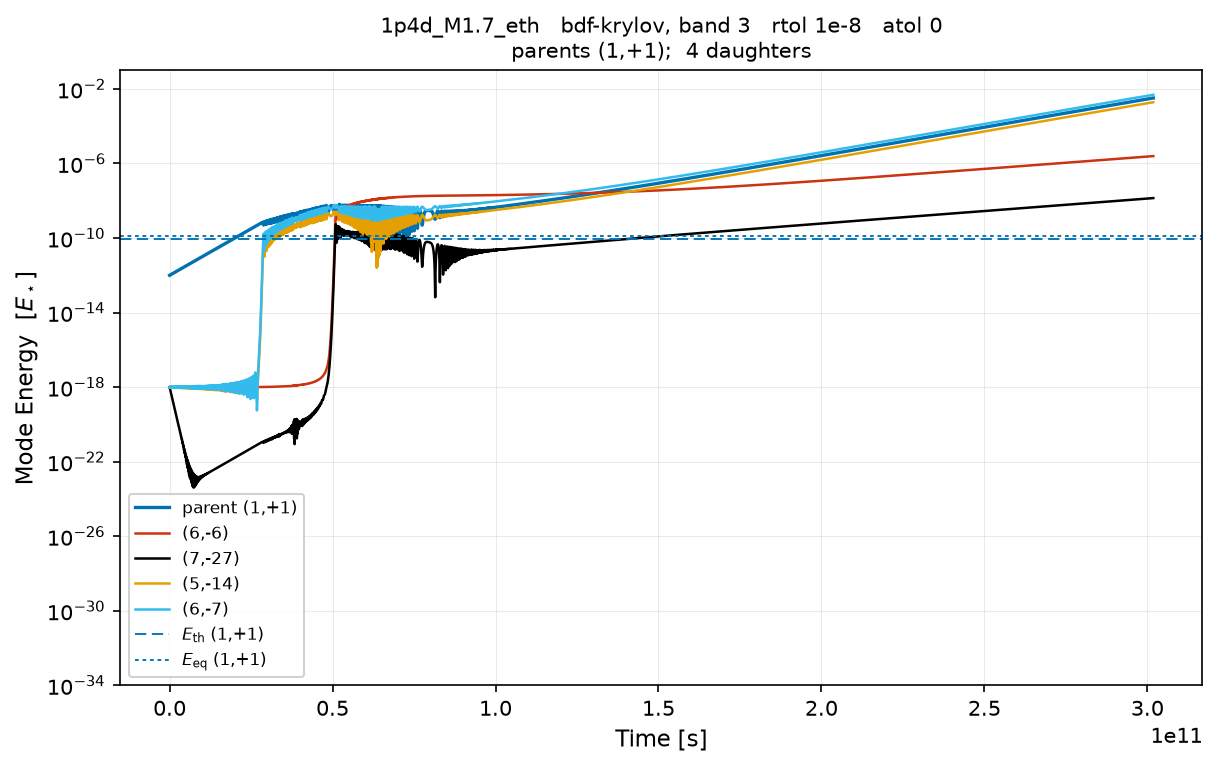
\includegraphics[width=0.21\textwidth,height=0.1323\textwidth]{../plots/krylov_b3/1p4d_M1.7_eth/r1e-8_a0.png} \\[-1pt]
 & \parbox[t]{0.21\textwidth}{\centering\scriptsize 66.98\,M steps, 163.0\,s, runaway} & \parbox[t]{0.21\textwidth}{\centering\scriptsize 66.99\,M steps, 172.6\,s, runaway} & \parbox[t]{0.21\textwidth}{\centering\scriptsize 66.99\,M steps, 176.3\,s, runaway} & \parbox[t]{0.21\textwidth}{\centering\scriptsize 66.99\,M steps, 170.4\,s, runaway} \\[2pt]
\rotatebox{90}{\parbox{0.1323\textwidth}{\centering\scriptsize\bfseries Adams, fixed point}} & 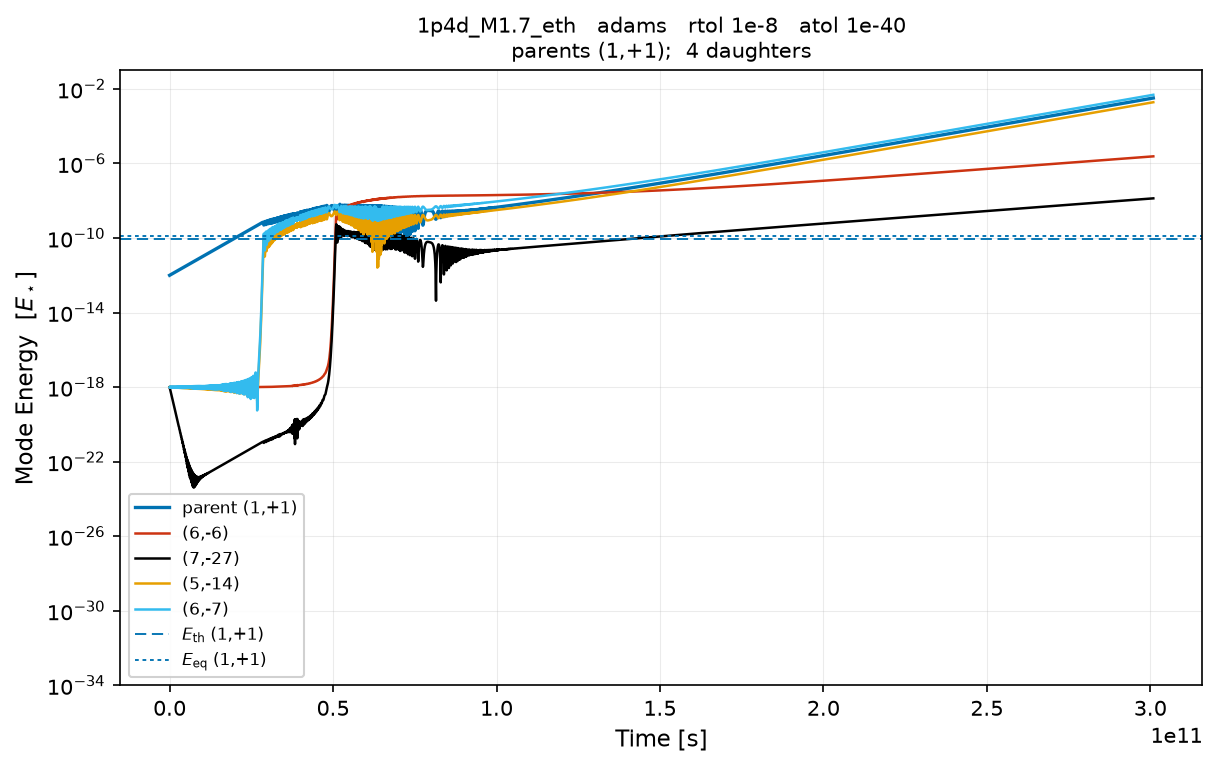
\includegraphics[width=0.21\textwidth,height=0.1323\textwidth]{../plots/adams/1p4d_M1.7_eth/r1e-8_a1e-40.png} & 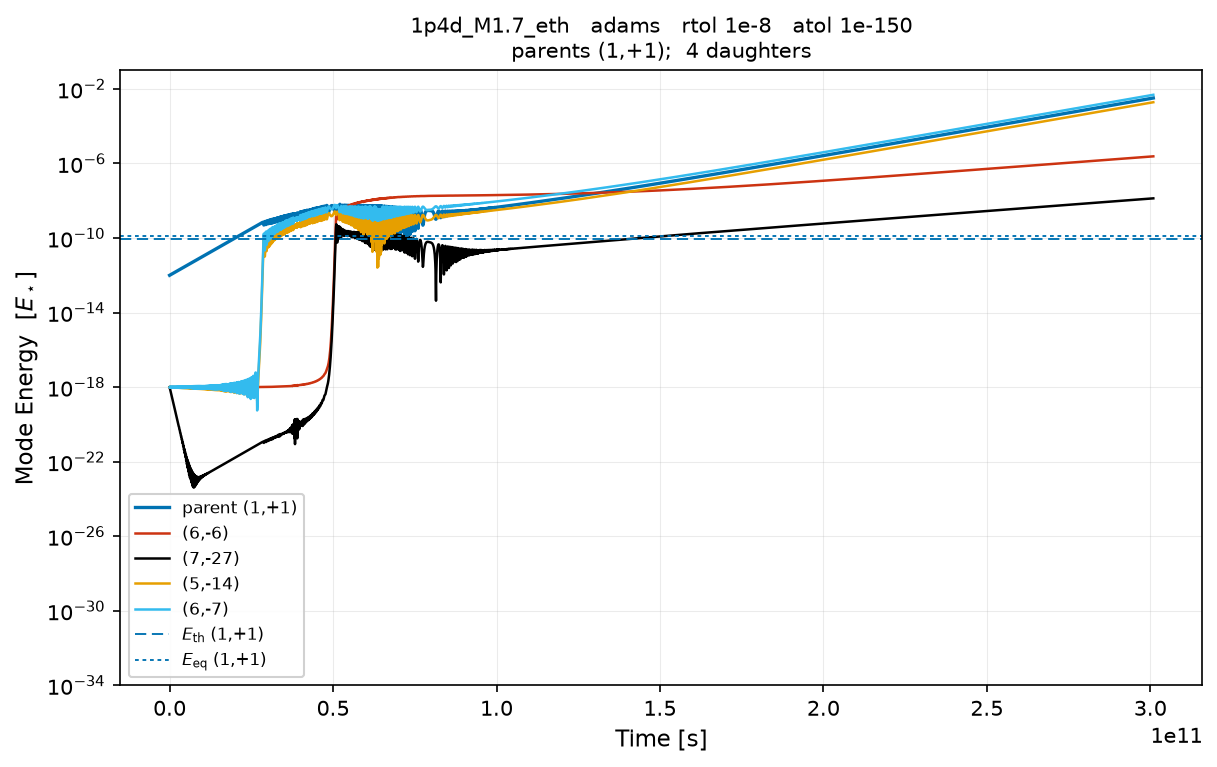
\includegraphics[width=0.21\textwidth,height=0.1323\textwidth]{../plots/adams/1p4d_M1.7_eth/r1e-8_a1e-150.png} & 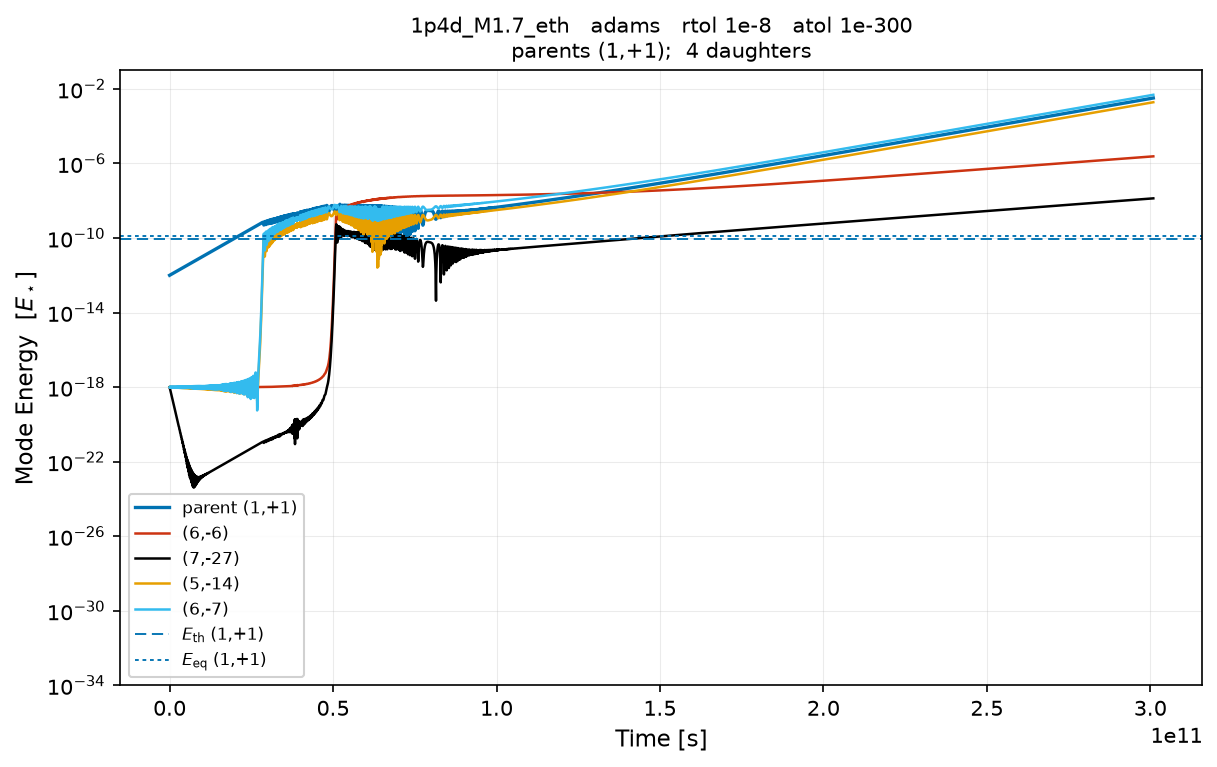
\includegraphics[width=0.21\textwidth,height=0.1323\textwidth]{../plots/adams/1p4d_M1.7_eth/r1e-8_a1e-300.png} & 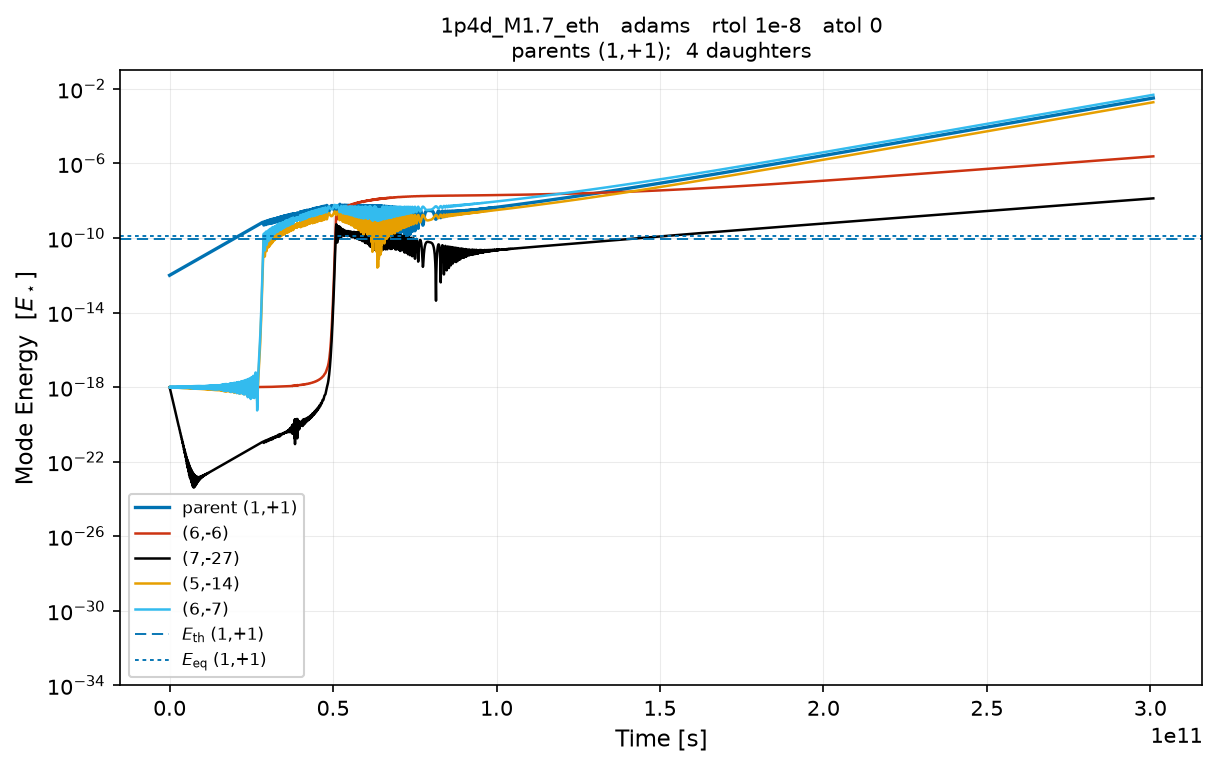
\includegraphics[width=0.21\textwidth,height=0.1323\textwidth]{../plots/adams/1p4d_M1.7_eth/r1e-8_a0.png} \\[-1pt]
 & \parbox[t]{0.21\textwidth}{\centering\scriptsize 42.69\,M steps, 64.2\,s, runaway} & \parbox[t]{0.21\textwidth}{\centering\scriptsize 42.69\,M steps, 50.1\,s, runaway} & \parbox[t]{0.21\textwidth}{\centering\scriptsize 42.69\,M steps, 52.2\,s, runaway} & \parbox[t]{0.21\textwidth}{\centering\scriptsize 42.69\,M steps, 42.8\,s, runaway} \\[2pt]
\end{tabular}\par}
\par\noindent{\scriptsize\setlength\tabcolsep{3.5pt}\renewcommand\arraystretch{0.92}
\begin{tabular}{@{}llllrrrrrrr@{}}
\toprule
integrator & atol & stop & $t_{\rm stop}$ [s] & steps & rejected & RHS & Jac. & NL it. & lin. it. & wall [s] \\
\midrule
rk8pd & $10^{-40}$ & runaway & $3.01\times10^{11}$ & 7.58\,M & 1.01\,M & 98.48\,M & -- & -- & -- & 19.8 \\
 & $10^{-150}$ & runaway & $3.01\times10^{11}$ & 7.58\,M & 1.01\,M & 98.48\,M & -- & -- & -- & 17.7 \\
 & $10^{-300}$ & runaway & $3.01\times10^{11}$ & 7.58\,M & 1.01\,M & 98.48\,M & -- & -- & -- & 18.4 \\
 & $0$ & runaway & $3.01\times10^{11}$ & 7.58\,M & 1.01\,M & 98.48\,M & -- & -- & -- & 19.8 \\
\addlinespace[2pt]
BDF, dense analytic Jacobian & $10^{-40}$ & runaway & $3.01\times10^{11}$ & 72.42\,M & 911.7\,k & 78.90\,M & 1.27\,M & 78.90\,M & -- & 74.9 \\
 & $10^{-150}$ & runaway & $3.01\times10^{11}$ & 72.41\,M & 918.0\,k & 78.93\,M & 1.27\,M & 78.93\,M & -- & 74.4 \\
 & $10^{-300}$ & runaway & $3.01\times10^{11}$ & 72.41\,M & 918.0\,k & 78.93\,M & 1.27\,M & 78.93\,M & -- & 122.1 \\
 & $0$ & runaway & $3.01\times10^{11}$ & 72.41\,M & 918.0\,k & 78.93\,M & 1.27\,M & 78.93\,M & -- & 90.0 \\
\addlinespace[2pt]
BDF-Krylov, band full & $10^{-40}$ & runaway & $3.02\times10^{11}$ & 69.74\,M & 989.6\,k & 163.10\,M & 1.19\,M & 76.22\,M & 75.01\,M & 133.2 \\
 & $10^{-150}$ & runaway & $3.02\times10^{11}$ & 69.63\,M & 1.00\,M & 162.99\,M & 1.19\,M & 76.17\,M & 74.96\,M & 134.7 \\
 & $10^{-300}$ & runaway & $3.02\times10^{11}$ & 69.63\,M & 1.00\,M & 162.99\,M & 1.19\,M & 76.17\,M & 74.96\,M & 109.1 \\
 & $0$ & runaway & $3.02\times10^{11}$ & 69.63\,M & 1.00\,M & 162.99\,M & 1.19\,M & 76.17\,M & 74.96\,M & 117.5 \\
\addlinespace[2pt]
BDF-Krylov, band 3 & $10^{-40}$ & runaway & $3.02\times10^{11}$ & 66.98\,M & 1.31\,M & 186.37\,M & 1.14\,M & 75.07\,M & 103.28\,M & 163.0 \\
 & $10^{-150}$ & runaway & $3.02\times10^{11}$ & 66.99\,M & 1.31\,M & 186.37\,M & 1.14\,M & 75.09\,M & 103.26\,M & 172.6 \\
 & $10^{-300}$ & runaway & $3.02\times10^{11}$ & 66.99\,M & 1.31\,M & 186.37\,M & 1.14\,M & 75.09\,M & 103.26\,M & 176.3 \\
 & $0$ & runaway & $3.02\times10^{11}$ & 66.99\,M & 1.31\,M & 186.37\,M & 1.14\,M & 75.09\,M & 103.26\,M & 170.4 \\
\addlinespace[2pt]
Adams, fixed point & $10^{-40}$ & runaway & $3.01\times10^{11}$ & 42.69\,M & 2.54\,M & 68.34\,M & -- & 68.34\,M & -- & 64.2 \\
 & $10^{-150}$ & runaway & $3.01\times10^{11}$ & 42.69\,M & 2.54\,M & 68.34\,M & -- & 68.34\,M & -- & 50.1 \\
 & $10^{-300}$ & runaway & $3.01\times10^{11}$ & 42.69\,M & 2.54\,M & 68.34\,M & -- & 68.34\,M & -- & 52.2 \\
 & $0$ & runaway & $3.01\times10^{11}$ & 42.69\,M & 2.54\,M & 68.34\,M & -- & 68.34\,M & -- & 42.8 \\
\bottomrule
\end{tabular}}

\clearpage
\subsection{\texttt{1p4d\_M2.0T\_eth}}\label{net:1p4d_M2.0T_eth}
\noindent\begin{minipage}[t]{0.43\textwidth}\vspace{0pt}\footnotesize
\begin{tabular}{@{}rrlrr@{}}
\toprule
id & gen & $(\ell,n)$ & $\omega$ [rad\,s$^{-1}$] & $\gamma$ [s$^{-1}$] \\
\midrule
0 & 0 & (2,$-$2) & $7.959\times10^{-4}$ & $-6.697\times10^{-11}$ \\
1 & 1 & (3,$-$31) & $1.287\times10^{-4}$ & $8.096\times10^{-11}$ \\
2 & 1 & (5,$-$8) & $6.672\times10^{-4}$ & $7.367\times10^{-13}$ \\
3 & 1 & (5,$-$9) & $6.216\times10^{-4}$ & $1.110\times10^{-12}$ \\
4 & 1 & (7,$-$50) & $1.743\times10^{-4}$ & $2.546\times10^{-9}$ \\
\bottomrule
\end{tabular}
\end{minipage}\hfill
\begin{minipage}[t]{0.55\textwidth}\vspace{0pt}\footnotesize
\textbf{Model} \texttt{dsct\_M2.0\_T7696}, rule eth, $N=4$, cut 0.15,
closure 0.005; 5 modes, 2 triplet(s).\\[2pt]
\textbf{Selecting pairs}\\ (2,$-$2) $\to$ (3,$-$31) + (5,$-$8): $\Delta/\omega_a=-3.69\times10^{-6}$, $\kappa=+0.215$, $E_{\rm th}=4.87\times10^{-12}$, $E_{\rm eq}=1.50\times10^{-10}$\\
(2,$-$2) $\to$ (5,$-$9) + (7,$-$50): $\Delta/\omega_a=7.51\times10^{-5}$, $\kappa=+0.053$, $E_{\rm th}=1.30\times10^{-9}$, $E_{\rm eq}=1.37\times10^{-9}$\\[2pt]

\end{minipage}

\par\smallskip{\centering\begin{tabular}{@{}c@{\hspace{2pt}}c@{\hspace{2pt}}c@{\hspace{2pt}}c@{\hspace{2pt}}c@{}}
 & \small atol $10^{-40}$ & \small atol $10^{-150}$ & \small atol $10^{-300}$ & \small atol $0$ \\[1pt]
\rotatebox{90}{\parbox{0.1323\textwidth}{\centering\scriptsize\bfseries rk8pd}} & 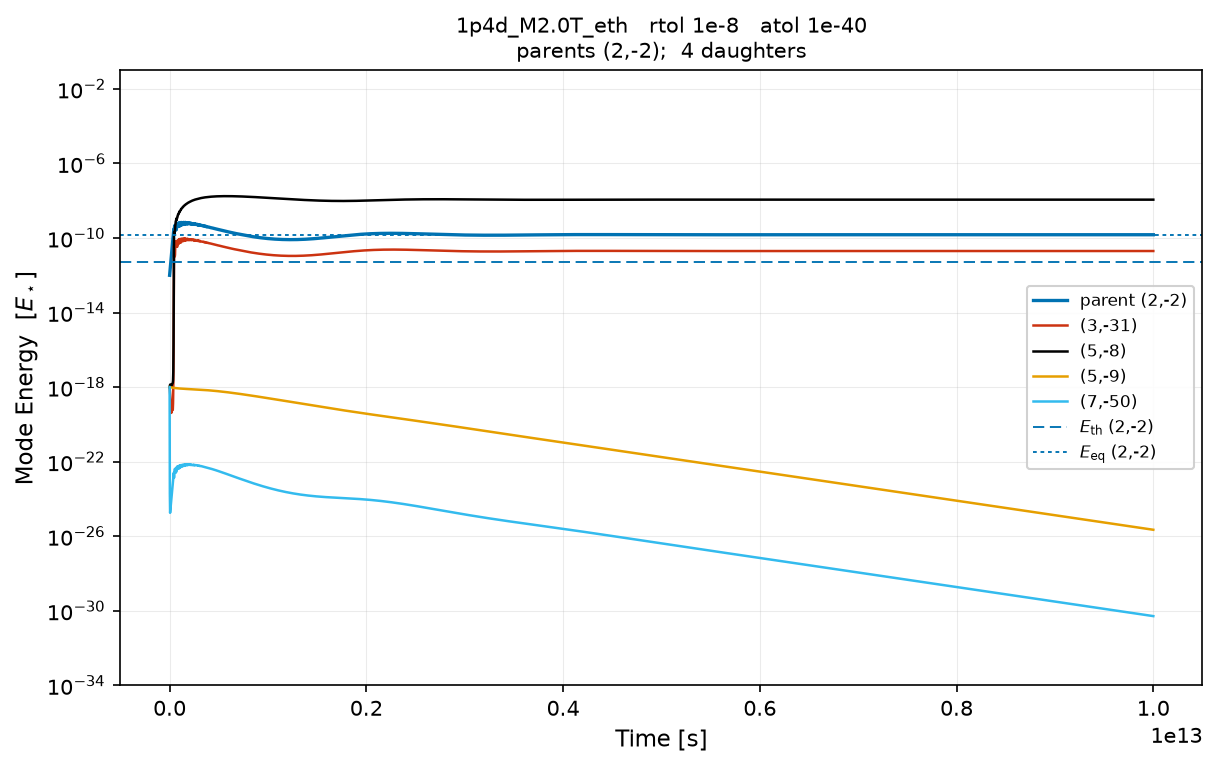
\includegraphics[width=0.21\textwidth,height=0.1323\textwidth]{../plots/rk8pd/1p4d_M2.0T_eth/r1e-8_a1e-40.png} & 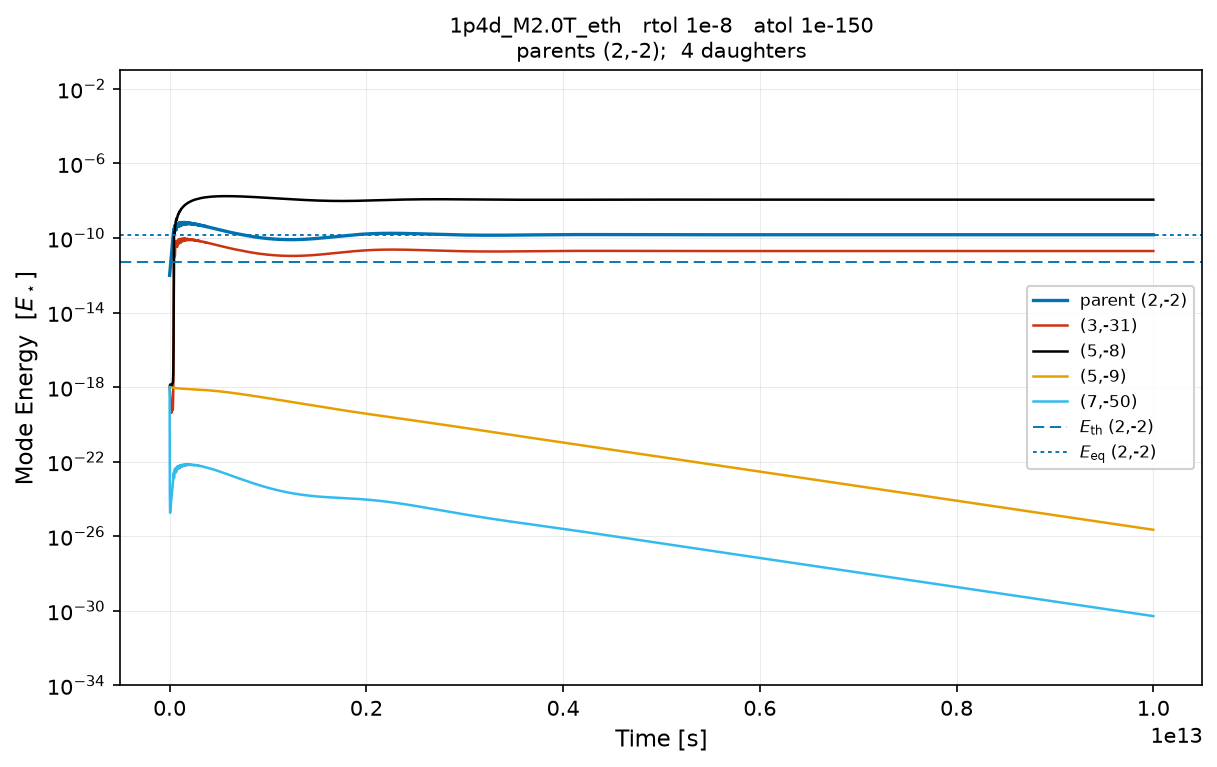
\includegraphics[width=0.21\textwidth,height=0.1323\textwidth]{../plots/rk8pd/1p4d_M2.0T_eth/r1e-8_a1e-150.png} & 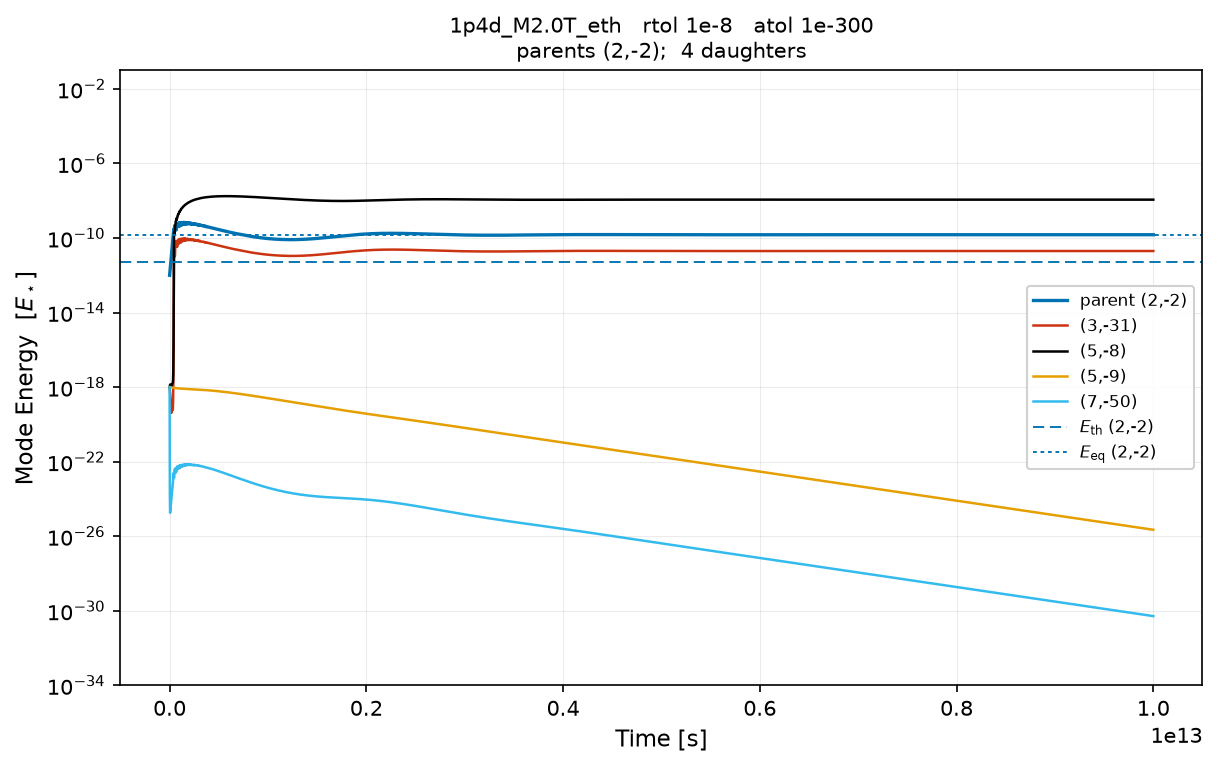
\includegraphics[width=0.21\textwidth,height=0.1323\textwidth]{../plots/rk8pd/1p4d_M2.0T_eth/r1e-8_a1e-300.png} & 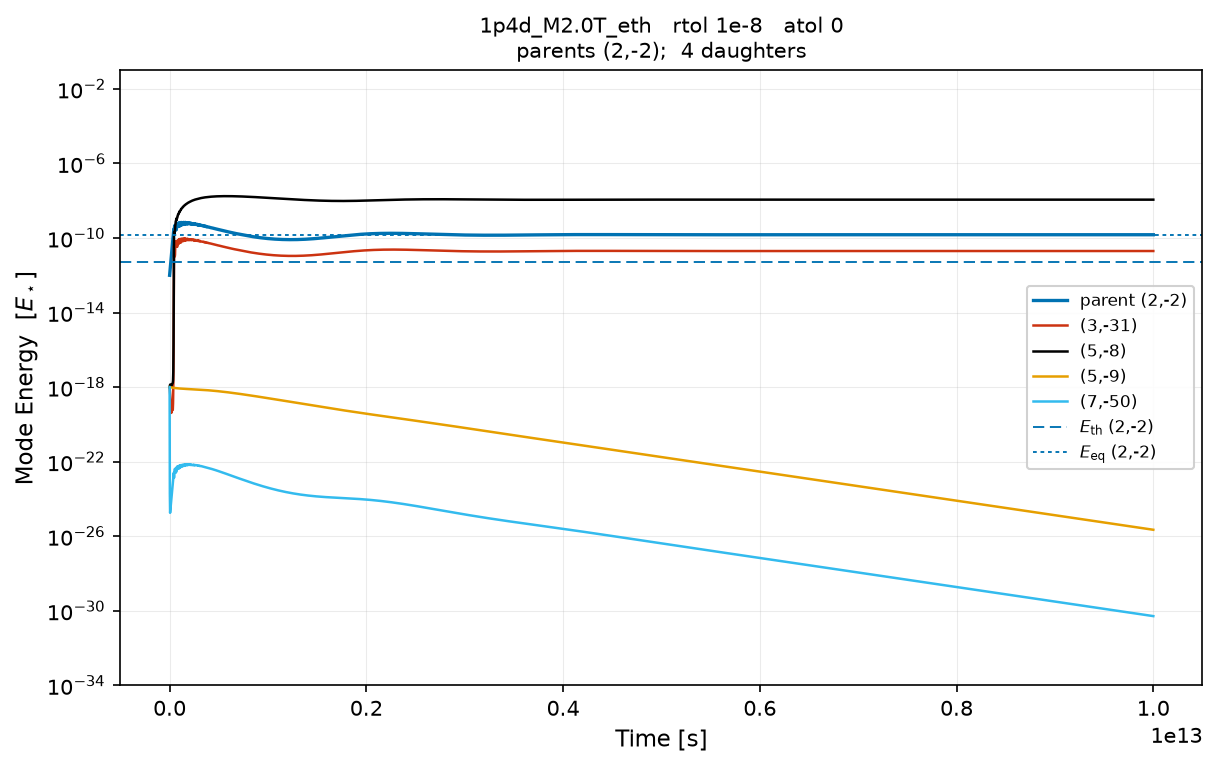
\includegraphics[width=0.21\textwidth,height=0.1323\textwidth]{../plots/rk8pd/1p4d_M2.0T_eth/r1e-8_a0.png} \\[-1pt]
 & \parbox[t]{0.21\textwidth}{\centering\scriptsize 618.4\,k steps, 1.8\,s} & \parbox[t]{0.21\textwidth}{\centering\scriptsize 618.5\,k steps, 2.5\,s} & \parbox[t]{0.21\textwidth}{\centering\scriptsize 618.5\,k steps, 1.2\,s} & \parbox[t]{0.21\textwidth}{\centering\scriptsize 618.5\,k steps, 2.7\,s} \\[2pt]
\rotatebox{90}{\parbox{0.1323\textwidth}{\centering\scriptsize\bfseries BDF, dense analytic Jacobian}} & 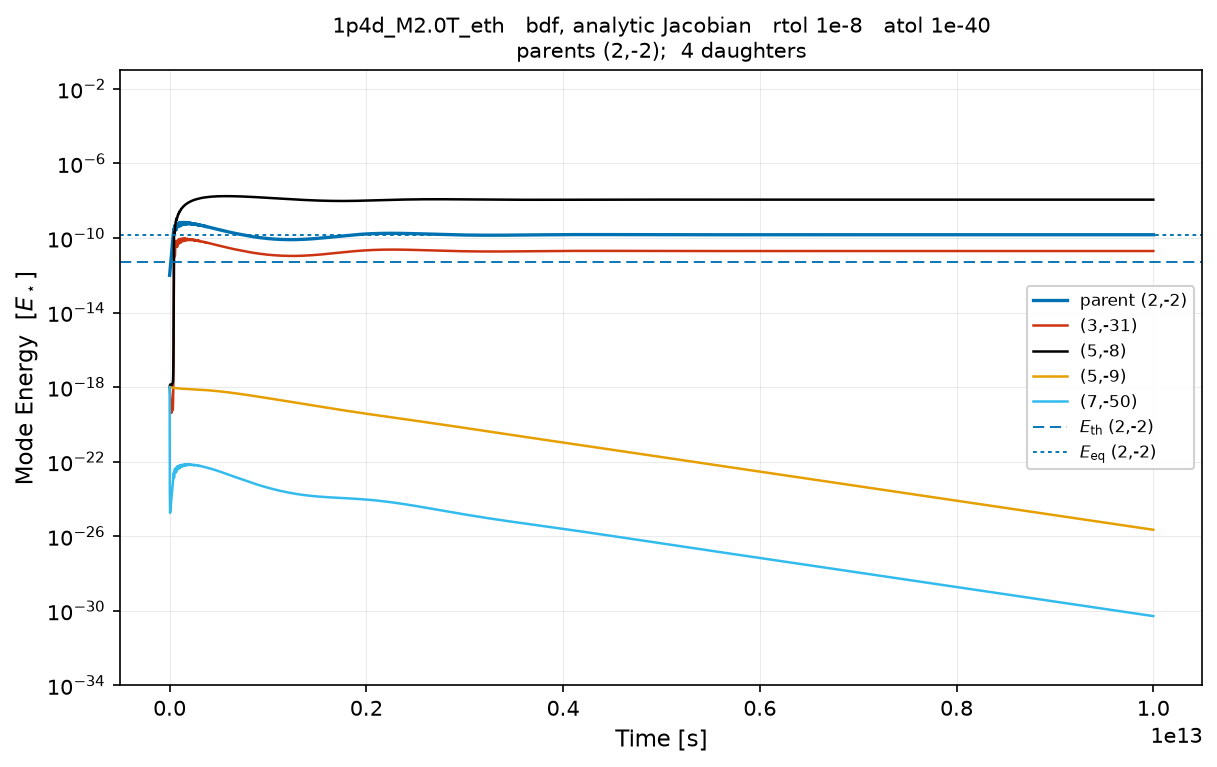
\includegraphics[width=0.21\textwidth,height=0.1323\textwidth]{../plots/bdf/1p4d_M2.0T_eth/r1e-8_a1e-40.png} & 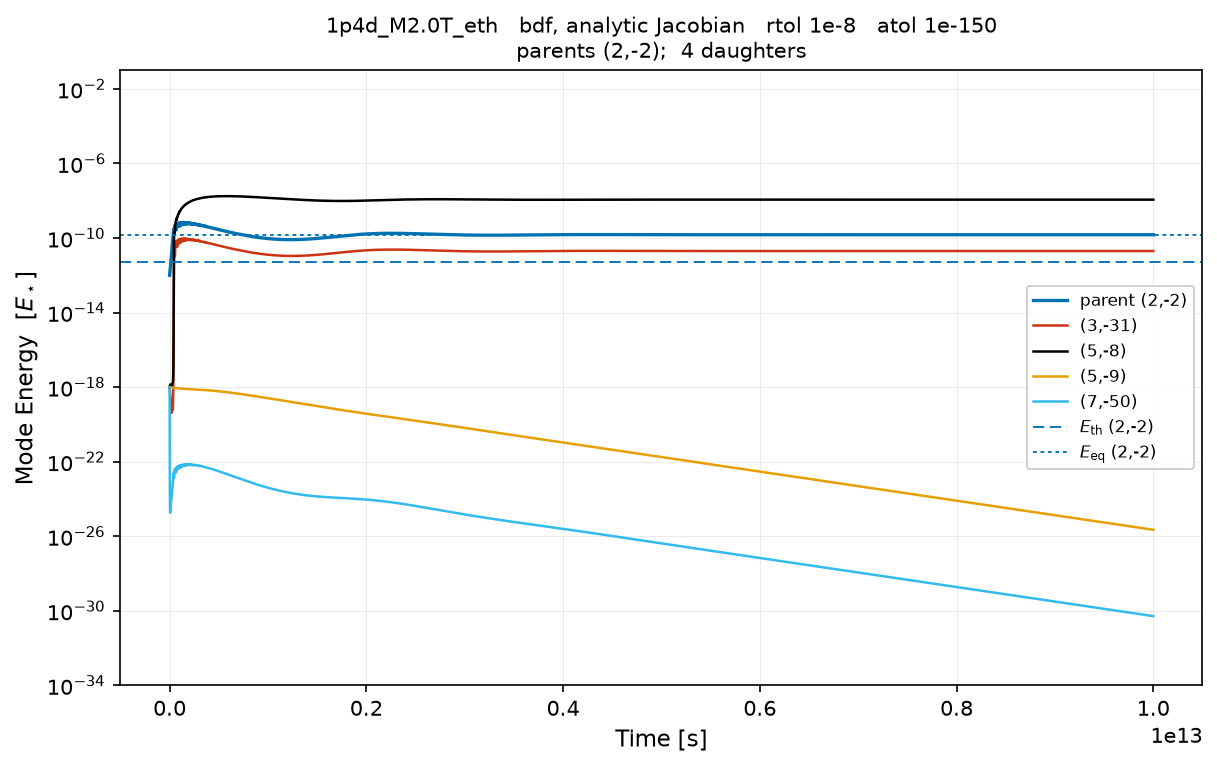
\includegraphics[width=0.21\textwidth,height=0.1323\textwidth]{../plots/bdf/1p4d_M2.0T_eth/r1e-8_a1e-150.png} & 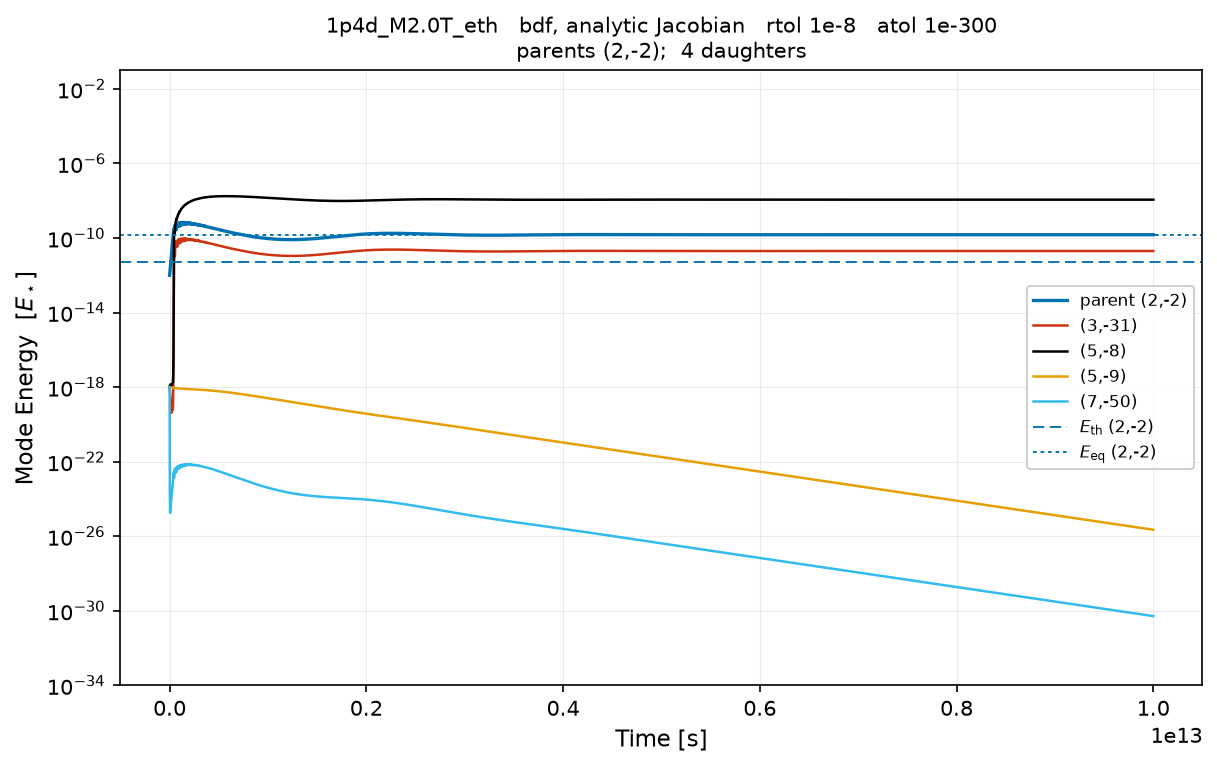
\includegraphics[width=0.21\textwidth,height=0.1323\textwidth]{../plots/bdf/1p4d_M2.0T_eth/r1e-8_a1e-300.png} & 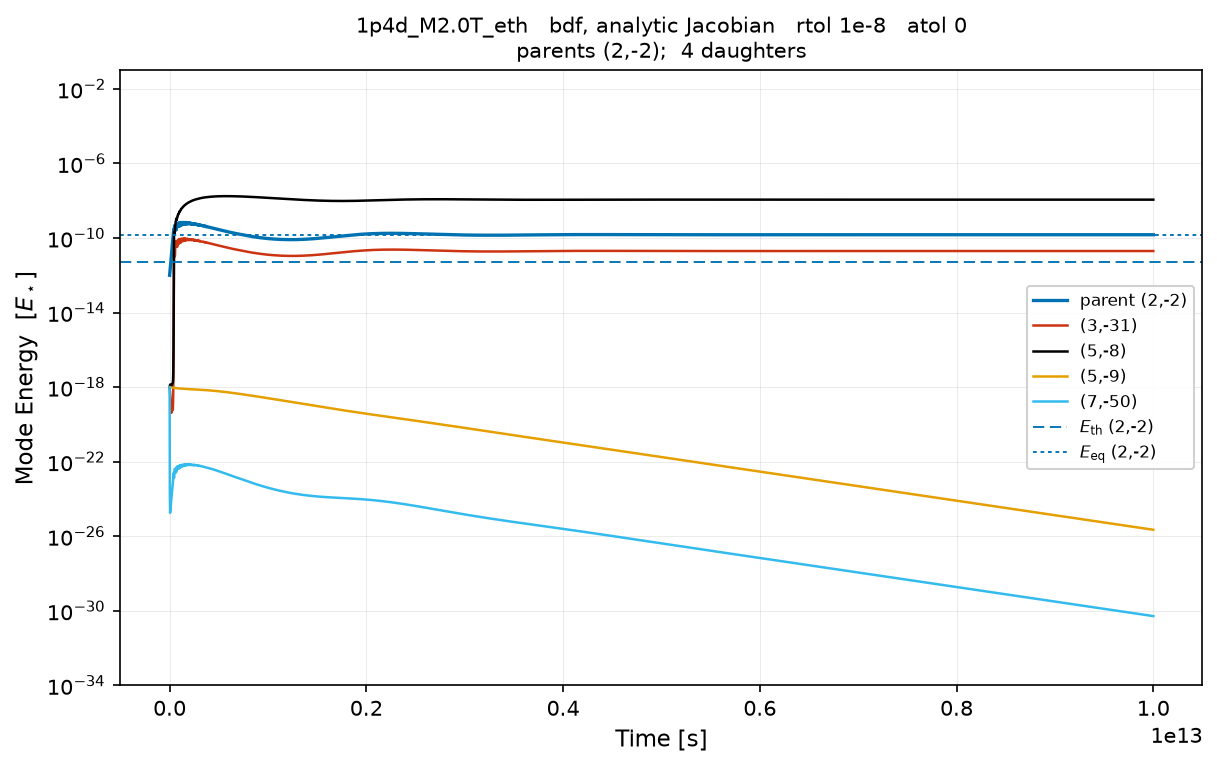
\includegraphics[width=0.21\textwidth,height=0.1323\textwidth]{../plots/bdf/1p4d_M2.0T_eth/r1e-8_a0.png} \\[-1pt]
 & \parbox[t]{0.21\textwidth}{\centering\scriptsize 9.43\,M steps, 8.3\,s} & \parbox[t]{0.21\textwidth}{\centering\scriptsize 9.42\,M steps, 9.5\,s} & \parbox[t]{0.21\textwidth}{\centering\scriptsize 9.42\,M steps, 9.7\,s} & \parbox[t]{0.21\textwidth}{\centering\scriptsize 9.42\,M steps, 11.1\,s} \\[2pt]
\rotatebox{90}{\parbox{0.1323\textwidth}{\centering\scriptsize\bfseries BDF-Krylov, band full}} & 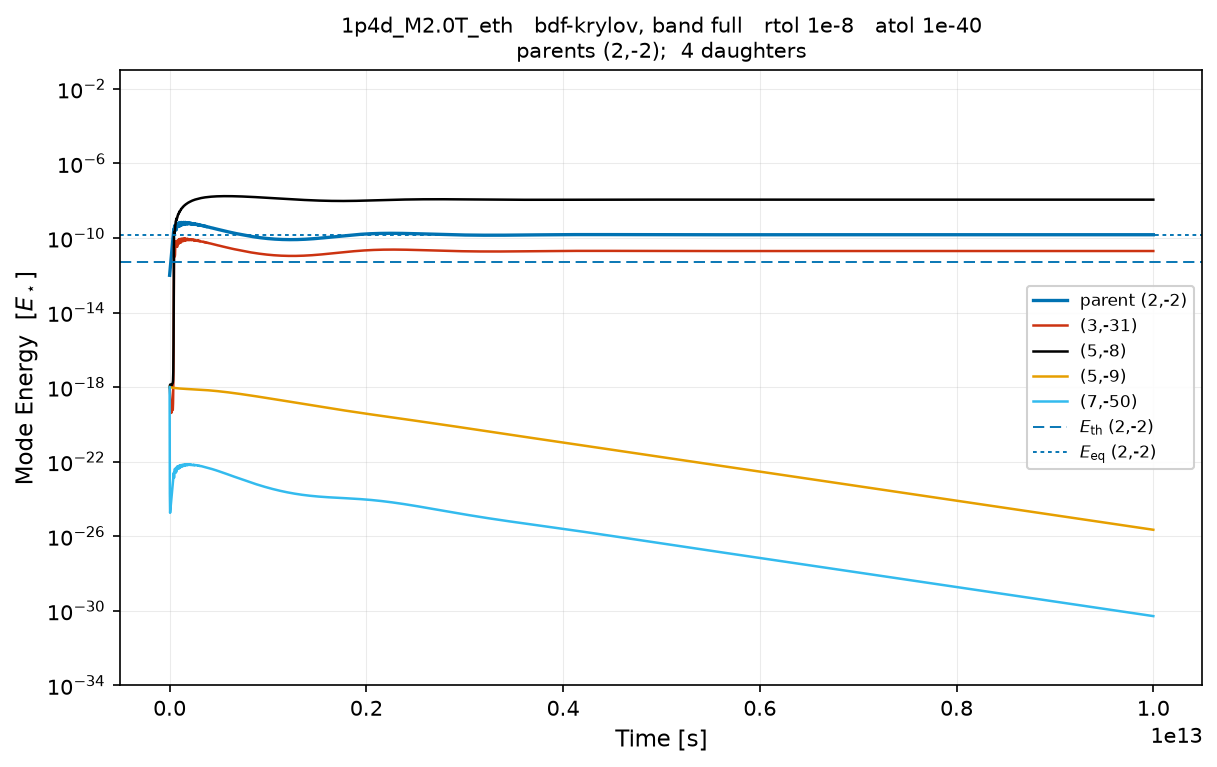
\includegraphics[width=0.21\textwidth,height=0.1323\textwidth]{../plots/krylov_full/1p4d_M2.0T_eth/r1e-8_a1e-40.png} & 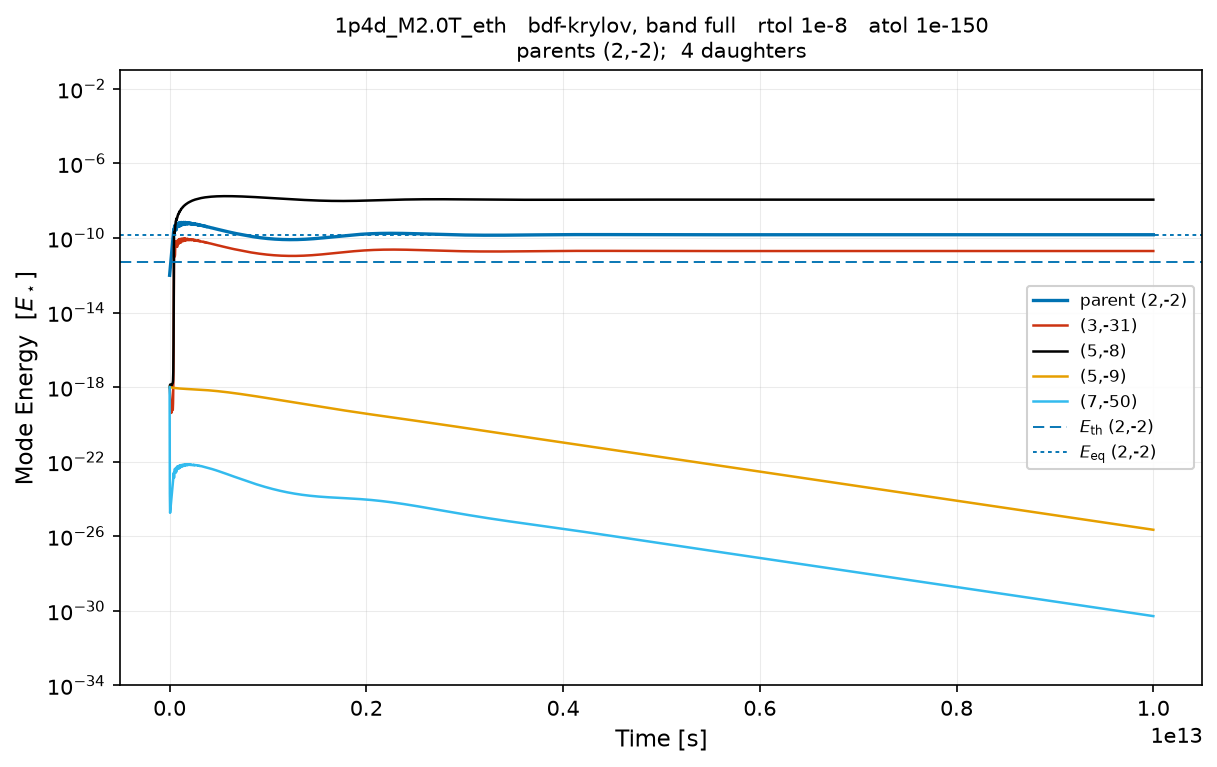
\includegraphics[width=0.21\textwidth,height=0.1323\textwidth]{../plots/krylov_full/1p4d_M2.0T_eth/r1e-8_a1e-150.png} & 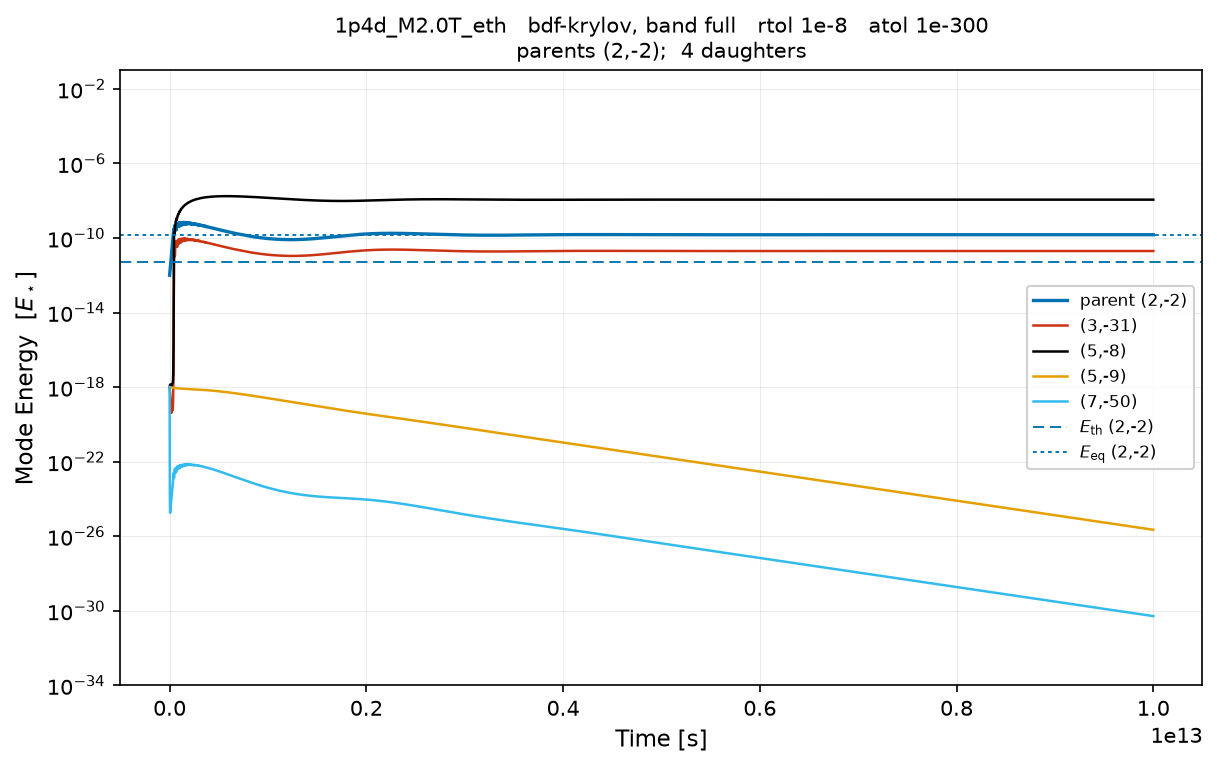
\includegraphics[width=0.21\textwidth,height=0.1323\textwidth]{../plots/krylov_full/1p4d_M2.0T_eth/r1e-8_a1e-300.png} & 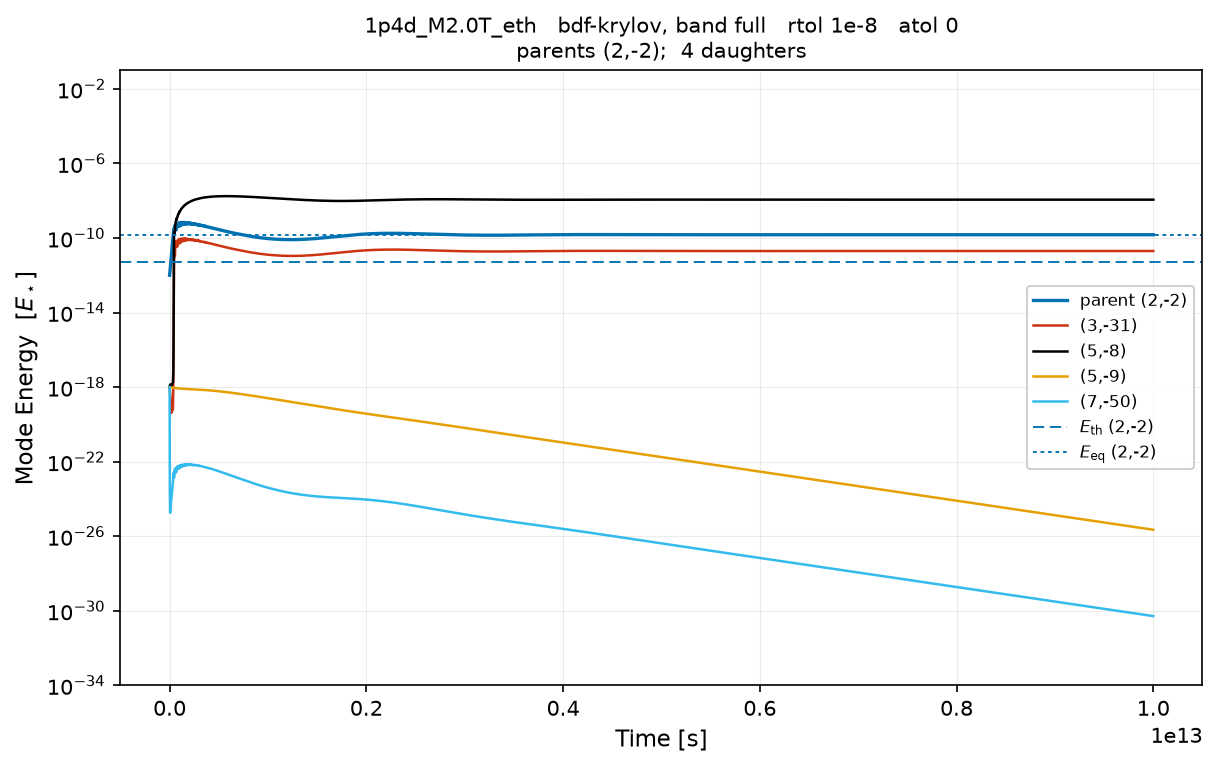
\includegraphics[width=0.21\textwidth,height=0.1323\textwidth]{../plots/krylov_full/1p4d_M2.0T_eth/r1e-8_a0.png} \\[-1pt]
 & \parbox[t]{0.21\textwidth}{\centering\scriptsize 9.43\,M steps, 23.2\,s} & \parbox[t]{0.21\textwidth}{\centering\scriptsize 9.43\,M steps, 23.7\,s} & \parbox[t]{0.21\textwidth}{\centering\scriptsize 9.43\,M steps, 13.0\,s} & \parbox[t]{0.21\textwidth}{\centering\scriptsize 9.43\,M steps, 14.4\,s} \\[2pt]
\rotatebox{90}{\parbox{0.1323\textwidth}{\centering\scriptsize\bfseries BDF-Krylov, band 3}} & 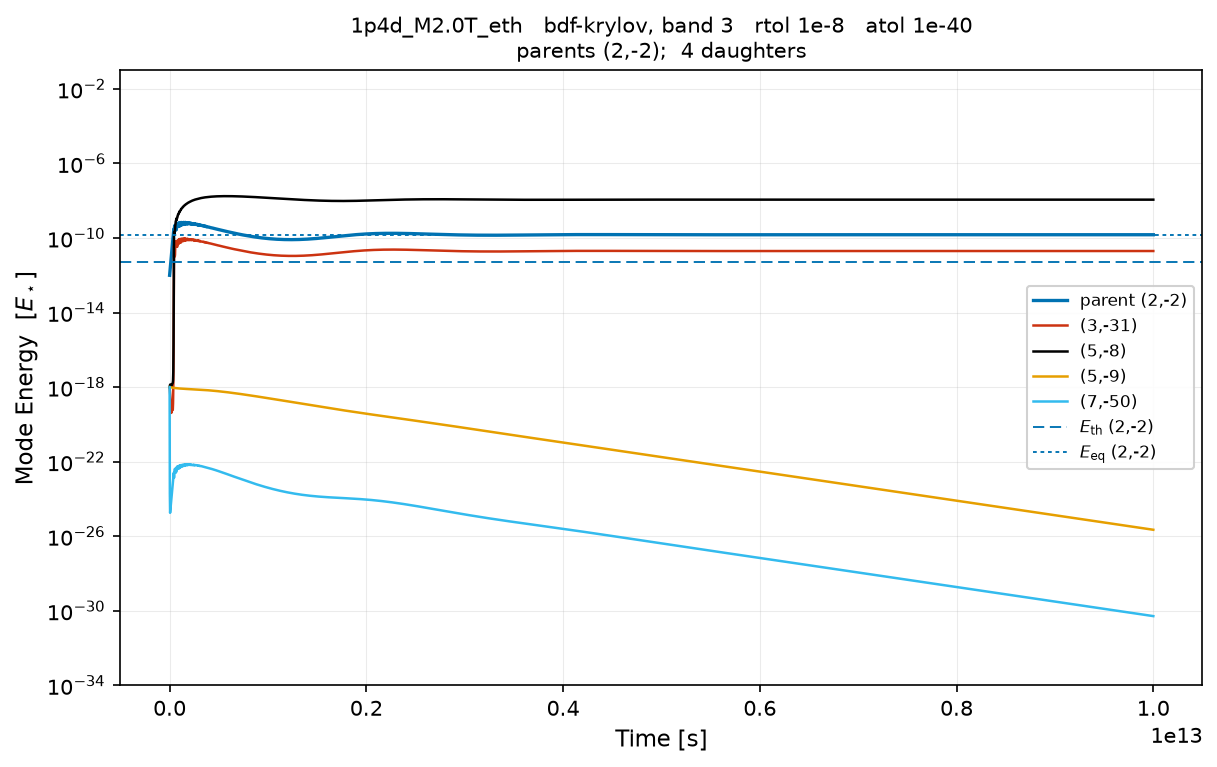
\includegraphics[width=0.21\textwidth,height=0.1323\textwidth]{../plots/krylov_b3/1p4d_M2.0T_eth/r1e-8_a1e-40.png} & 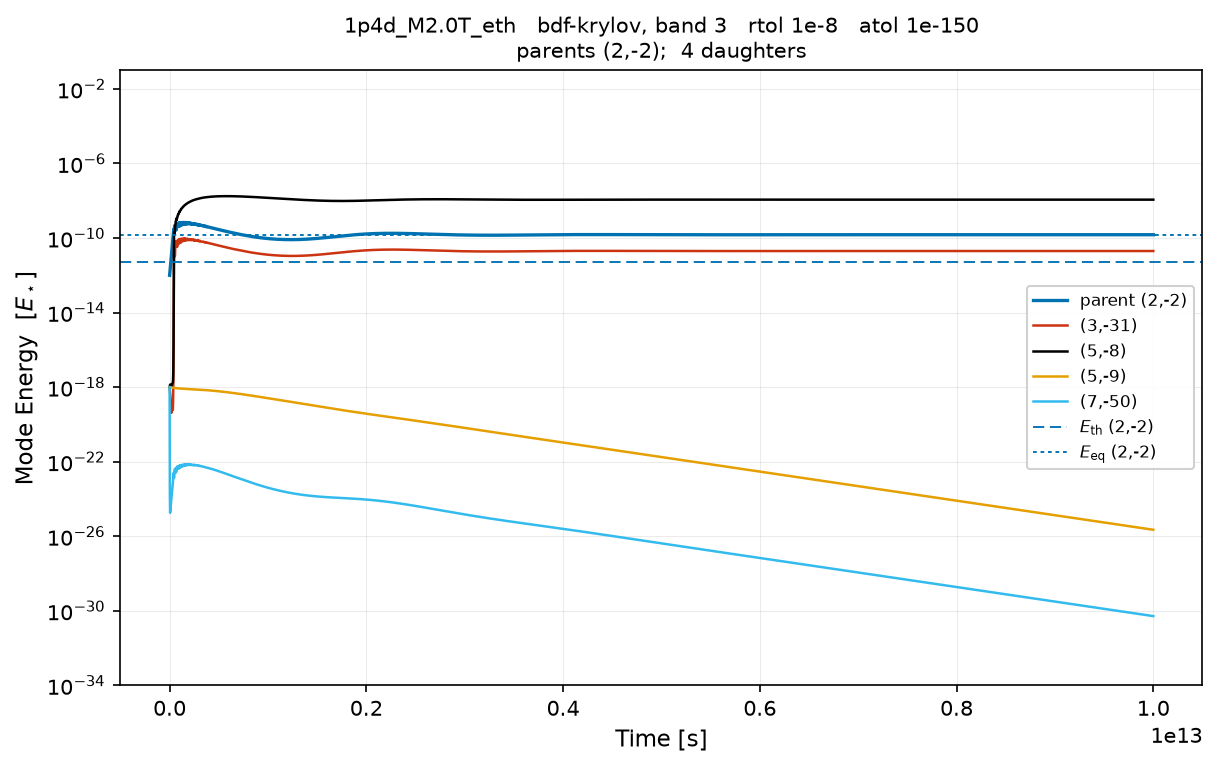
\includegraphics[width=0.21\textwidth,height=0.1323\textwidth]{../plots/krylov_b3/1p4d_M2.0T_eth/r1e-8_a1e-150.png} & 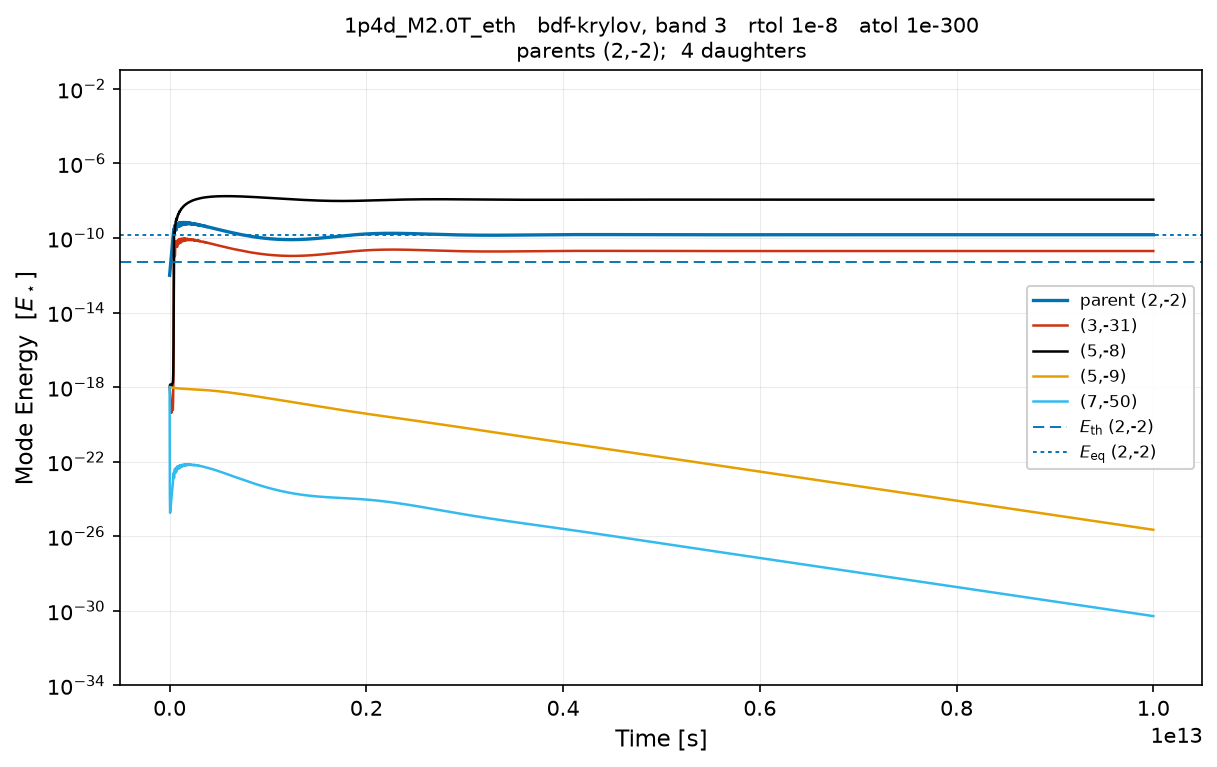
\includegraphics[width=0.21\textwidth,height=0.1323\textwidth]{../plots/krylov_b3/1p4d_M2.0T_eth/r1e-8_a1e-300.png} & 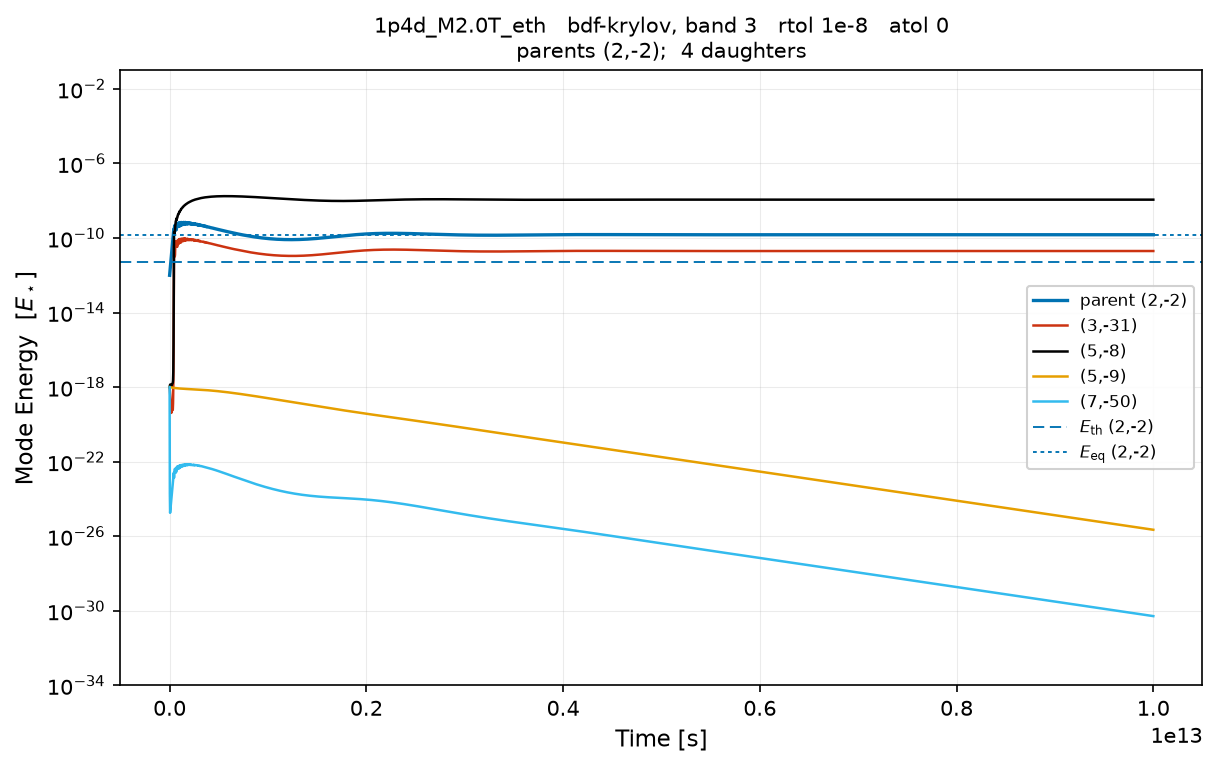
\includegraphics[width=0.21\textwidth,height=0.1323\textwidth]{../plots/krylov_b3/1p4d_M2.0T_eth/r1e-8_a0.png} \\[-1pt]
 & \parbox[t]{0.21\textwidth}{\centering\scriptsize 8.99\,M steps, 20.7\,s} & \parbox[t]{0.21\textwidth}{\centering\scriptsize 8.99\,M steps, 15.9\,s} & \parbox[t]{0.21\textwidth}{\centering\scriptsize 8.99\,M steps, 23.0\,s} & \parbox[t]{0.21\textwidth}{\centering\scriptsize 8.99\,M steps, 21.5\,s} \\[2pt]
\rotatebox{90}{\parbox{0.1323\textwidth}{\centering\scriptsize\bfseries Adams, fixed point}} & 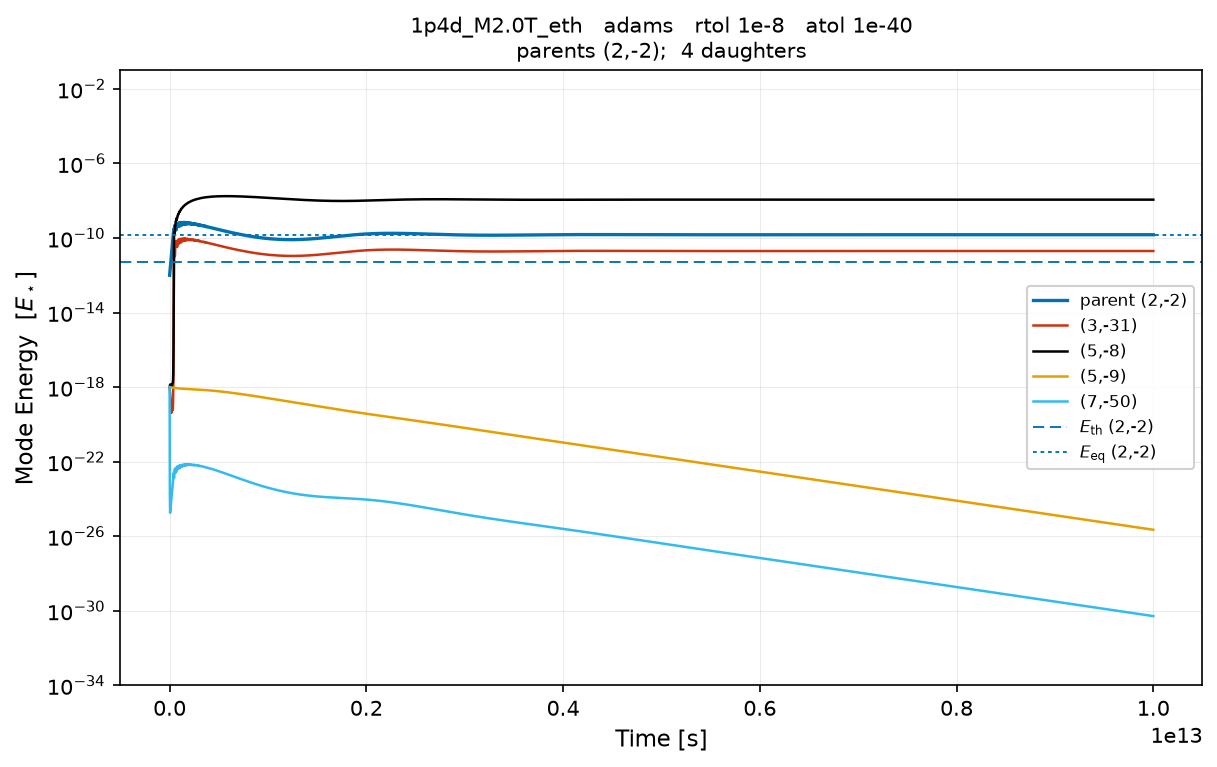
\includegraphics[width=0.21\textwidth,height=0.1323\textwidth]{../plots/adams/1p4d_M2.0T_eth/r1e-8_a1e-40.png} & 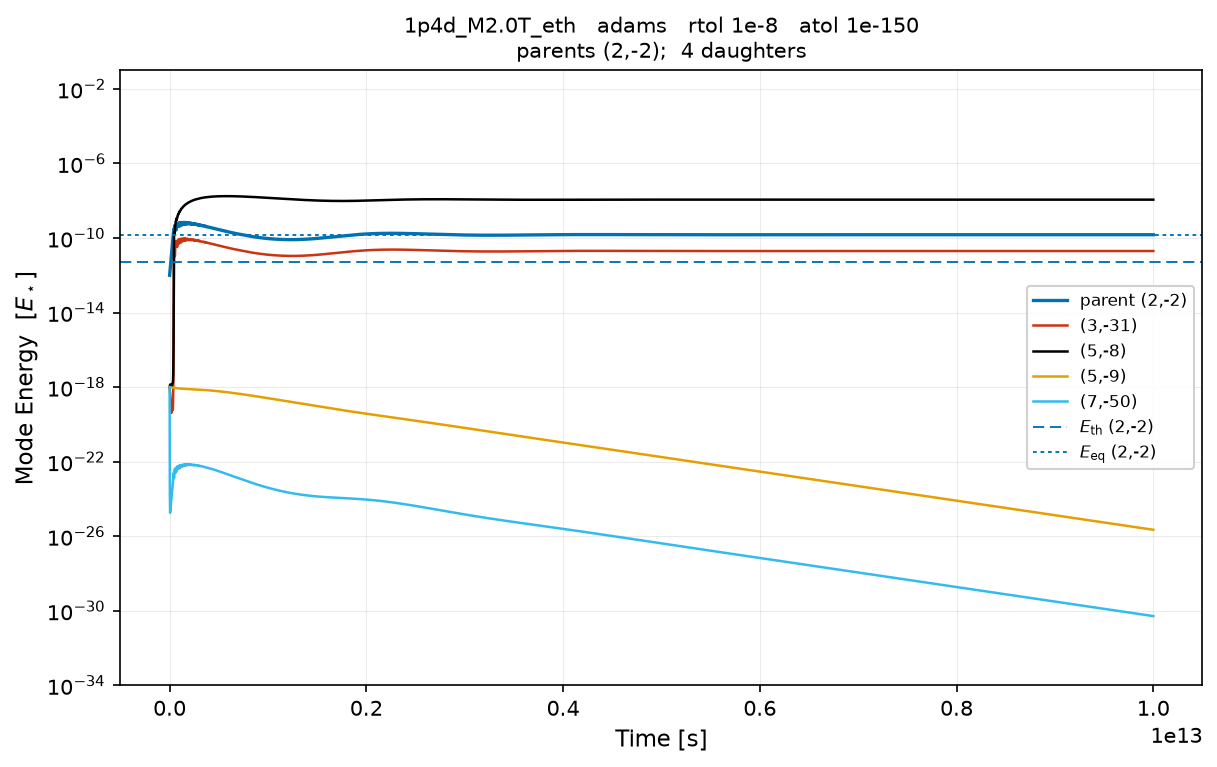
\includegraphics[width=0.21\textwidth,height=0.1323\textwidth]{../plots/adams/1p4d_M2.0T_eth/r1e-8_a1e-150.png} & 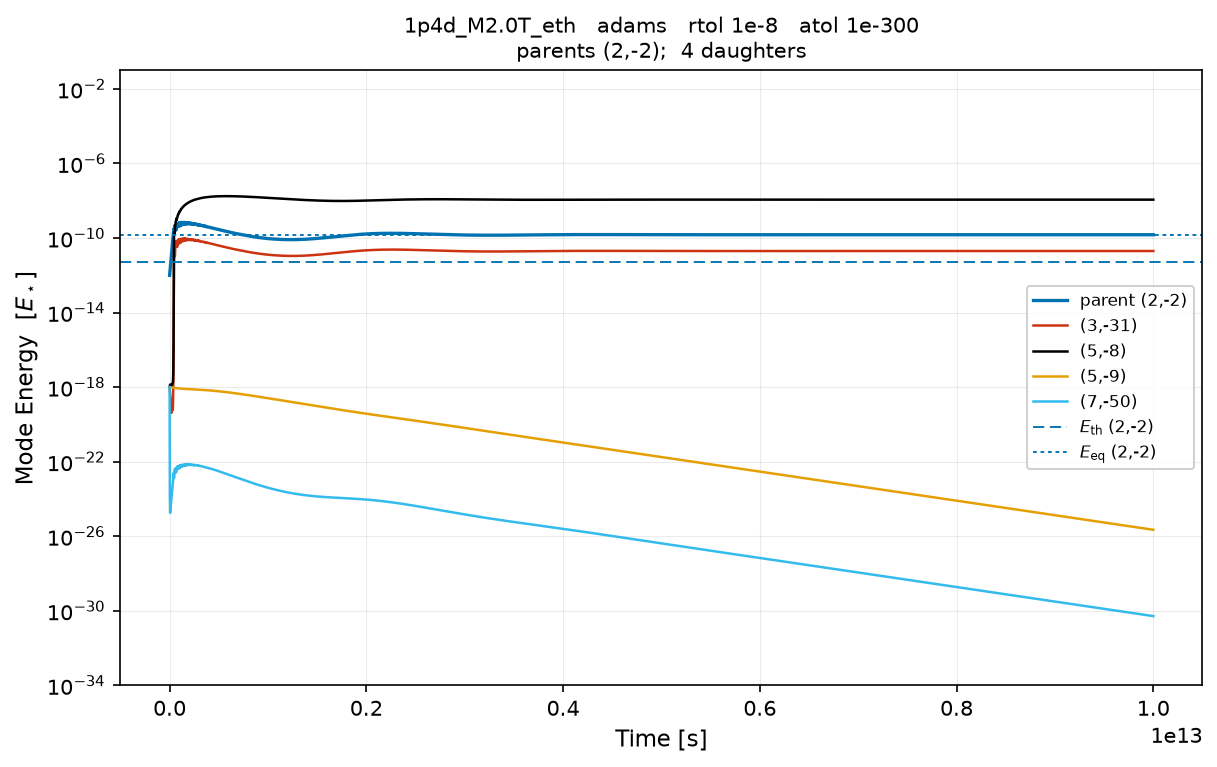
\includegraphics[width=0.21\textwidth,height=0.1323\textwidth]{../plots/adams/1p4d_M2.0T_eth/r1e-8_a1e-300.png} & 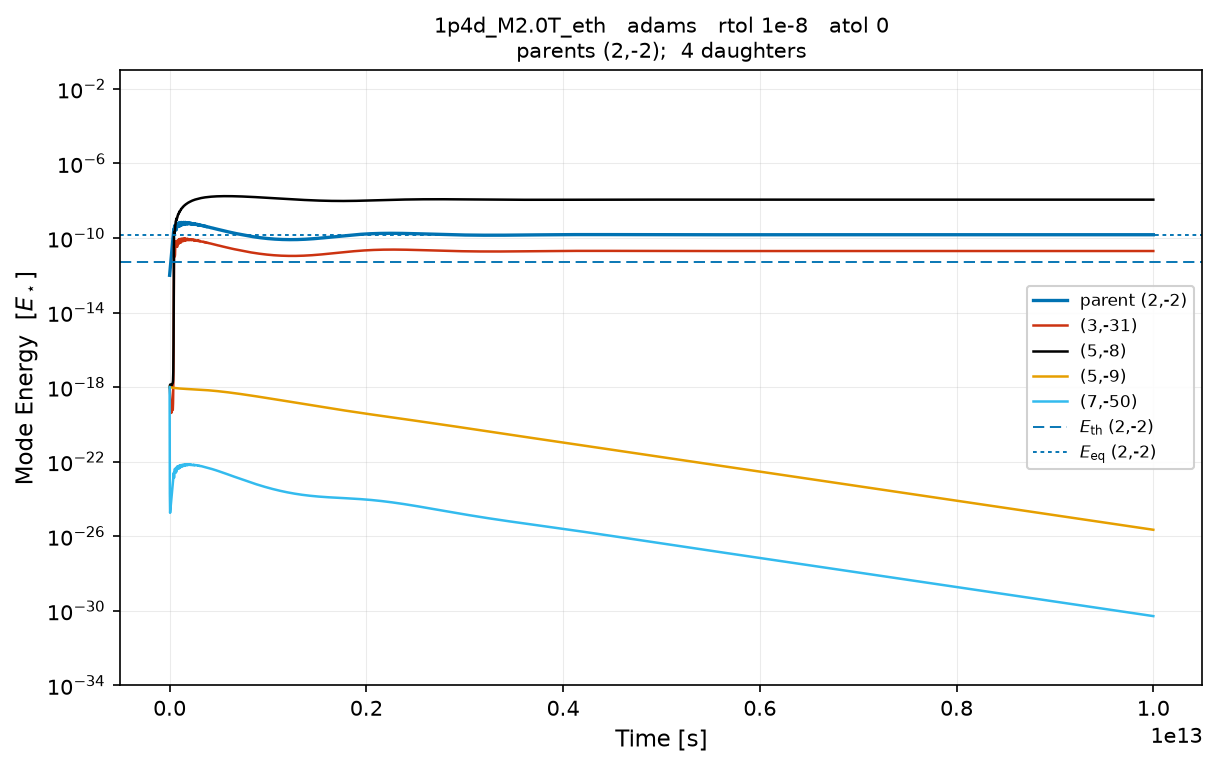
\includegraphics[width=0.21\textwidth,height=0.1323\textwidth]{../plots/adams/1p4d_M2.0T_eth/r1e-8_a0.png} \\[-1pt]
 & \parbox[t]{0.21\textwidth}{\centering\scriptsize 4.10\,M steps, 6.9\,s} & \parbox[t]{0.21\textwidth}{\centering\scriptsize 4.11\,M steps, 6.2\,s} & \parbox[t]{0.21\textwidth}{\centering\scriptsize 4.11\,M steps, 4.1\,s} & \parbox[t]{0.21\textwidth}{\centering\scriptsize 4.11\,M steps, 4.3\,s} \\[2pt]
\end{tabular}\par}
\par\noindent{\scriptsize\setlength\tabcolsep{3.5pt}\renewcommand\arraystretch{0.92}
\begin{tabular}{@{}llllrrrrrrr@{}}
\toprule
integrator & atol & stop & $t_{\rm stop}$ [s] & steps & rejected & RHS & Jac. & NL it. & lin. it. & wall [s] \\
\midrule
rk8pd & $10^{-40}$ & end & $1.00\times10^{13}$ & 618.4\,k & 18.4\,k & 8.04\,M & -- & -- & -- & 1.8 \\
 & $10^{-150}$ & end & $1.00\times10^{13}$ & 618.5\,k & 18.4\,k & 8.04\,M & -- & -- & -- & 2.5 \\
 & $10^{-300}$ & end & $1.00\times10^{13}$ & 618.5\,k & 18.4\,k & 8.04\,M & -- & -- & -- & 1.2 \\
 & $0$ & end & $1.00\times10^{13}$ & 618.5\,k & 18.4\,k & 8.04\,M & -- & -- & -- & 2.7 \\
\addlinespace[2pt]
BDF, dense analytic Jacobian & $10^{-40}$ & end & $1.00\times10^{13}$ & 9.43\,M & 89.6\,k & 10.13\,M & 167.6\,k & 10.13\,M & -- & 8.3 \\
 & $10^{-150}$ & end & $1.00\times10^{13}$ & 9.42\,M & 89.5\,k & 10.12\,M & 167.4\,k & 10.12\,M & -- & 9.5 \\
 & $10^{-300}$ & end & $1.00\times10^{13}$ & 9.42\,M & 89.5\,k & 10.12\,M & 167.4\,k & 10.12\,M & -- & 9.7 \\
 & $0$ & end & $1.00\times10^{13}$ & 9.42\,M & 89.5\,k & 10.12\,M & 167.4\,k & 10.12\,M & -- & 11.1 \\
\addlinespace[2pt]
BDF-Krylov, band full & $10^{-40}$ & end & $1.00\times10^{13}$ & 9.43\,M & 89.3\,k & 21.30\,M & 167.6\,k & 10.12\,M & 9.49\,M & 23.2 \\
 & $10^{-150}$ & end & $1.00\times10^{13}$ & 9.43\,M & 89.6\,k & 21.29\,M & 167.5\,k & 10.12\,M & 9.49\,M & 23.7 \\
 & $10^{-300}$ & end & $1.00\times10^{13}$ & 9.43\,M & 89.6\,k & 21.29\,M & 167.5\,k & 10.12\,M & 9.49\,M & 13.0 \\
 & $0$ & end & $1.00\times10^{13}$ & 9.43\,M & 89.6\,k & 21.29\,M & 167.5\,k & 10.12\,M & 9.49\,M & 14.4 \\
\addlinespace[2pt]
BDF-Krylov, band 3 & $10^{-40}$ & end & $1.00\times10^{13}$ & 8.99\,M & 122.0\,k & 21.67\,M & 160.4\,k & 9.86\,M & 10.69\,M & 20.7 \\
 & $10^{-150}$ & end & $1.00\times10^{13}$ & 8.99\,M & 122.3\,k & 21.67\,M & 160.4\,k & 9.86\,M & 10.68\,M & 15.9 \\
 & $10^{-300}$ & end & $1.00\times10^{13}$ & 8.99\,M & 122.3\,k & 21.67\,M & 160.4\,k & 9.86\,M & 10.68\,M & 23.0 \\
 & $0$ & end & $1.00\times10^{13}$ & 8.99\,M & 122.3\,k & 21.67\,M & 160.4\,k & 9.86\,M & 10.68\,M & 21.5 \\
\addlinespace[2pt]
Adams, fixed point & $10^{-40}$ & end & $1.00\times10^{13}$ & 4.10\,M & 287.6\,k & 6.43\,M & -- & 6.42\,M & -- & 6.9 \\
 & $10^{-150}$ & end & $1.00\times10^{13}$ & 4.11\,M & 283.9\,k & 6.44\,M & -- & 6.44\,M & -- & 6.2 \\
 & $10^{-300}$ & end & $1.00\times10^{13}$ & 4.11\,M & 283.9\,k & 6.44\,M & -- & 6.44\,M & -- & 4.1 \\
 & $0$ & end & $1.00\times10^{13}$ & 4.11\,M & 283.9\,k & 6.44\,M & -- & 6.44\,M & -- & 4.3 \\
\bottomrule
\end{tabular}}

\clearpage
\subsection{\texttt{1p4d\_M2.0\_eth}}\label{net:1p4d_M2.0_eth}
\noindent\begin{minipage}[t]{0.43\textwidth}\vspace{0pt}\footnotesize
\begin{tabular}{@{}rrlrr@{}}
\toprule
id & gen & $(\ell,n)$ & $\omega$ [rad\,s$^{-1}$] & $\gamma$ [s$^{-1}$] \\
\midrule
0 & 0 & (1,$-$1) & $7.581\times10^{-4}$ & $-2.276\times10^{-10}$ \\
1 & 1 & (4,$-$38) & $1.383\times10^{-4}$ & $2.224\times10^{-10}$ \\
2 & 1 & (5,$-$9) & $6.198\times10^{-4}$ & $4.584\times10^{-13}$ \\
3 & 1 & (4,$-$8) & $5.844\times10^{-4}$ & $4.902\times10^{-13}$ \\
4 & 1 & (5,$-$37) & $1.736\times10^{-4}$ & $1.454\times10^{-10}$ \\
\bottomrule
\end{tabular}
\end{minipage}\hfill
\begin{minipage}[t]{0.55\textwidth}\vspace{0pt}\footnotesize
\textbf{Model} \texttt{dsct\_M2.0}, rule eth, $N=4$, cut 0.15,
closure 0.005; 5 modes, 2 triplet(s).\\[2pt]
\textbf{Selecting pairs}\\ (1,$-$1) $\to$ (4,$-$38) + (5,$-$9): $\Delta/\omega_a=6.73\times10^{-5}$, $\kappa=+0.342$, $E_{\rm th}=1.33\times10^{-10}$, no $E_{\rm eq}$\\
(1,$-$1) $\to$ (4,$-$8) + (5,$-$37): $\Delta/\omega_a=-1.23\times10^{-4}$, $\kappa=+0.171$, $E_{\rm th}=2.46\times10^{-9}$, no $E_{\rm eq}$\\[2pt]

\end{minipage}

\par\smallskip{\centering\begin{tabular}{@{}c@{\hspace{2pt}}c@{\hspace{2pt}}c@{\hspace{2pt}}c@{\hspace{2pt}}c@{}}
 & \small atol $10^{-40}$ & \small atol $10^{-150}$ & \small atol $10^{-300}$ & \small atol $0$ \\[1pt]
\rotatebox{90}{\parbox{0.1323\textwidth}{\centering\scriptsize\bfseries rk8pd}} & 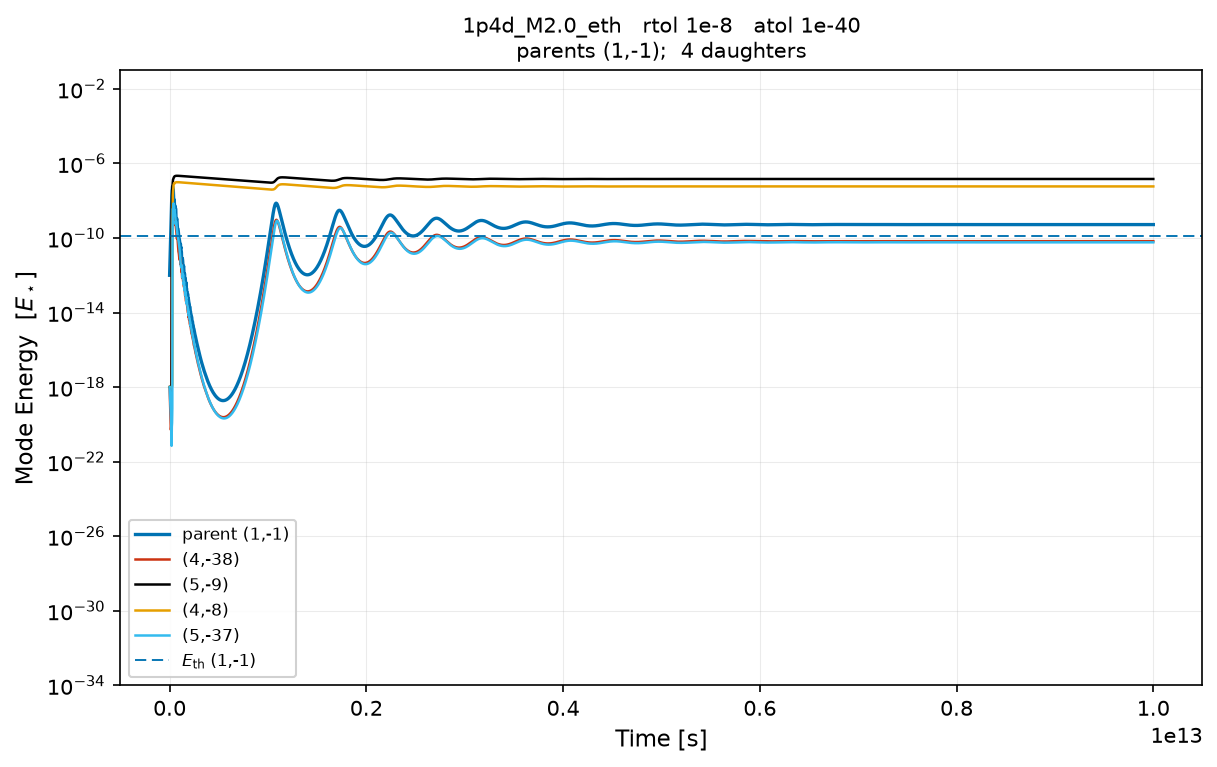
\includegraphics[width=0.21\textwidth,height=0.1323\textwidth]{../plots/rk8pd/1p4d_M2.0_eth/r1e-8_a1e-40.png} & 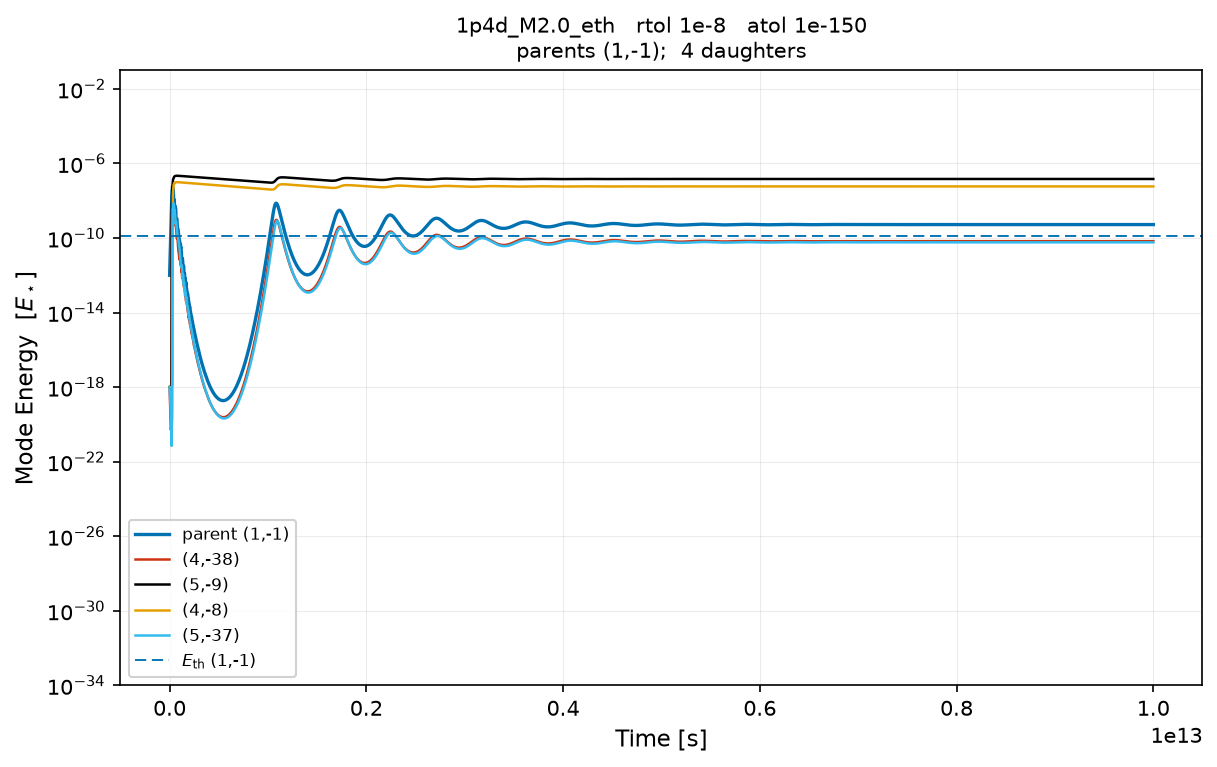
\includegraphics[width=0.21\textwidth,height=0.1323\textwidth]{../plots/rk8pd/1p4d_M2.0_eth/r1e-8_a1e-150.png} & 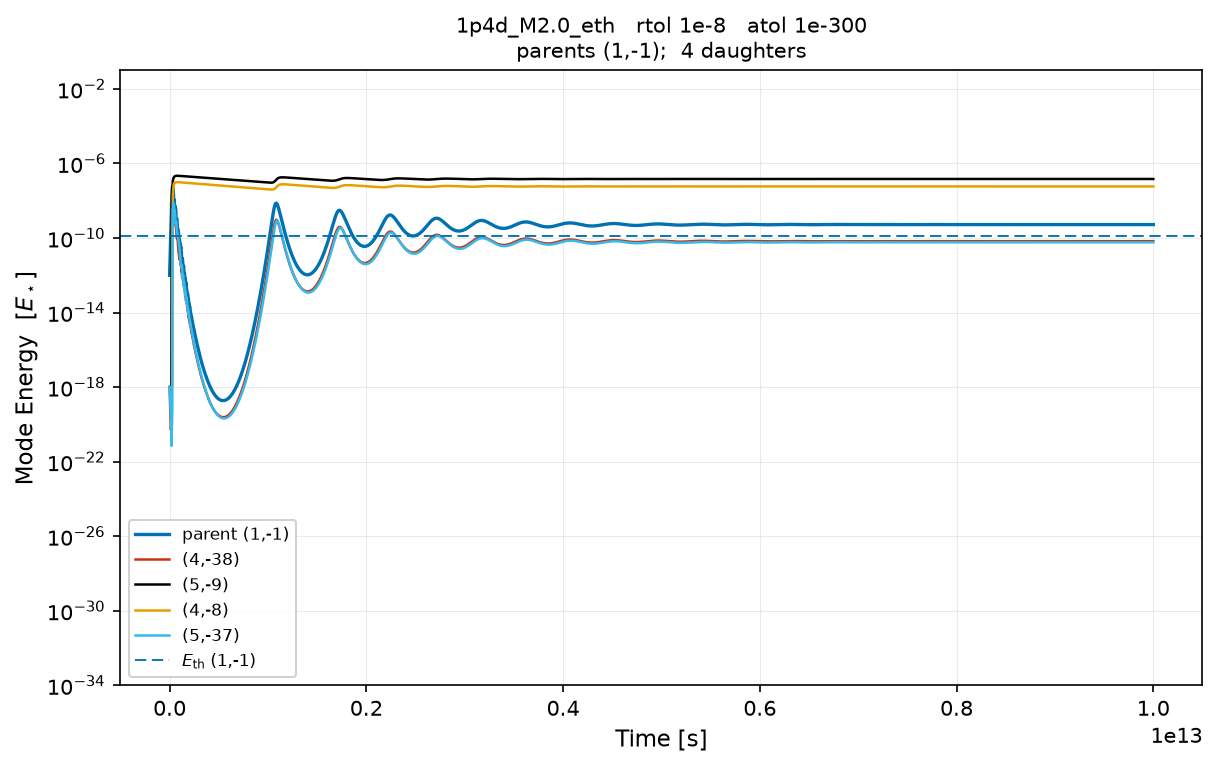
\includegraphics[width=0.21\textwidth,height=0.1323\textwidth]{../plots/rk8pd/1p4d_M2.0_eth/r1e-8_a1e-300.png} & 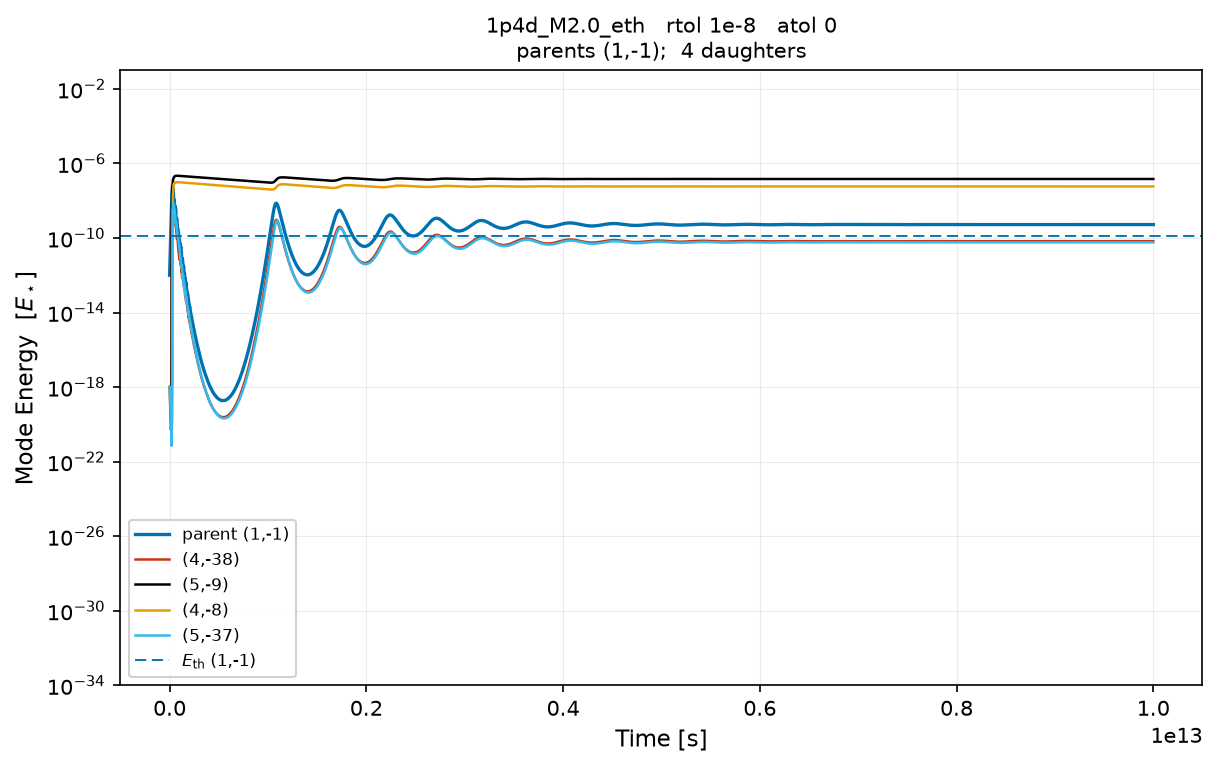
\includegraphics[width=0.21\textwidth,height=0.1323\textwidth]{../plots/rk8pd/1p4d_M2.0_eth/r1e-8_a0.png} \\[-1pt]
 & \parbox[t]{0.21\textwidth}{\centering\scriptsize 2.41\,M steps, 5.2\,s} & \parbox[t]{0.21\textwidth}{\centering\scriptsize 2.41\,M steps, 10.5\,s} & \parbox[t]{0.21\textwidth}{\centering\scriptsize 2.41\,M steps, 7.6\,s} & \parbox[t]{0.21\textwidth}{\centering\scriptsize 2.41\,M steps, 10.1\,s} \\[2pt]
\rotatebox{90}{\parbox{0.1323\textwidth}{\centering\scriptsize\bfseries BDF, dense analytic Jacobian}} & 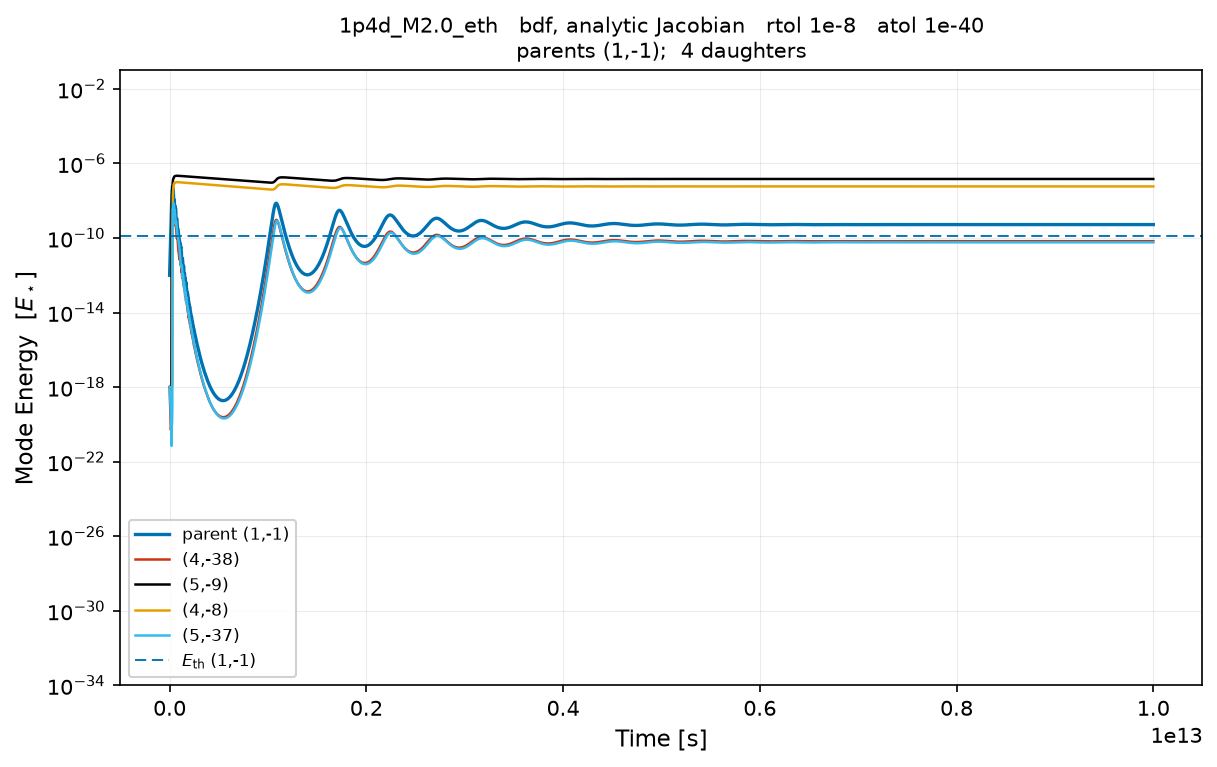
\includegraphics[width=0.21\textwidth,height=0.1323\textwidth]{../plots/bdf/1p4d_M2.0_eth/r1e-8_a1e-40.png} & 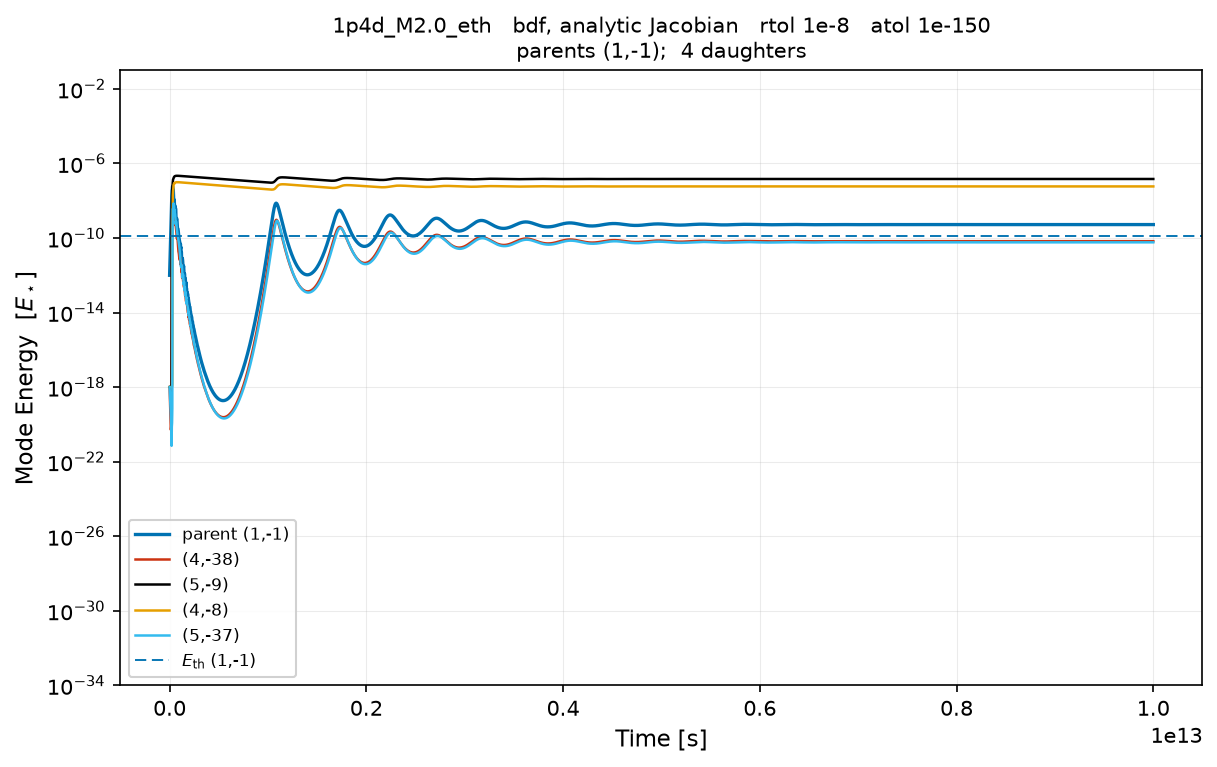
\includegraphics[width=0.21\textwidth,height=0.1323\textwidth]{../plots/bdf/1p4d_M2.0_eth/r1e-8_a1e-150.png} & 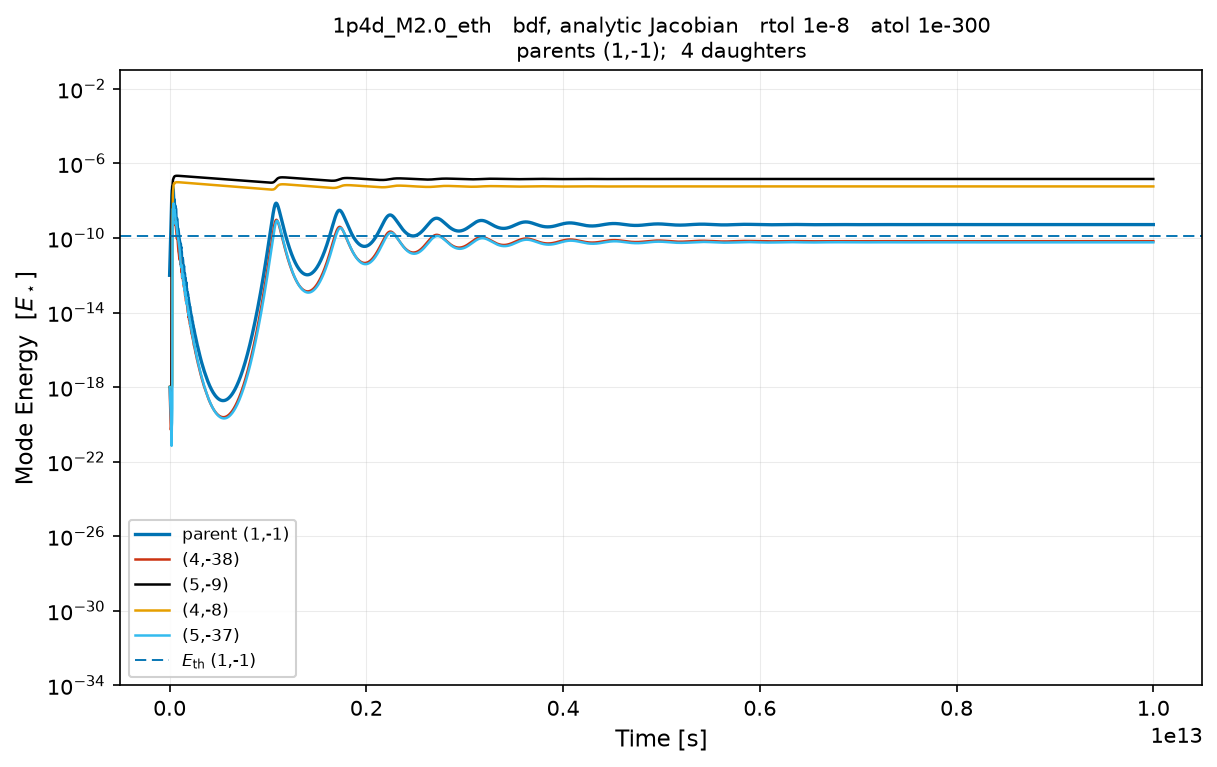
\includegraphics[width=0.21\textwidth,height=0.1323\textwidth]{../plots/bdf/1p4d_M2.0_eth/r1e-8_a1e-300.png} & 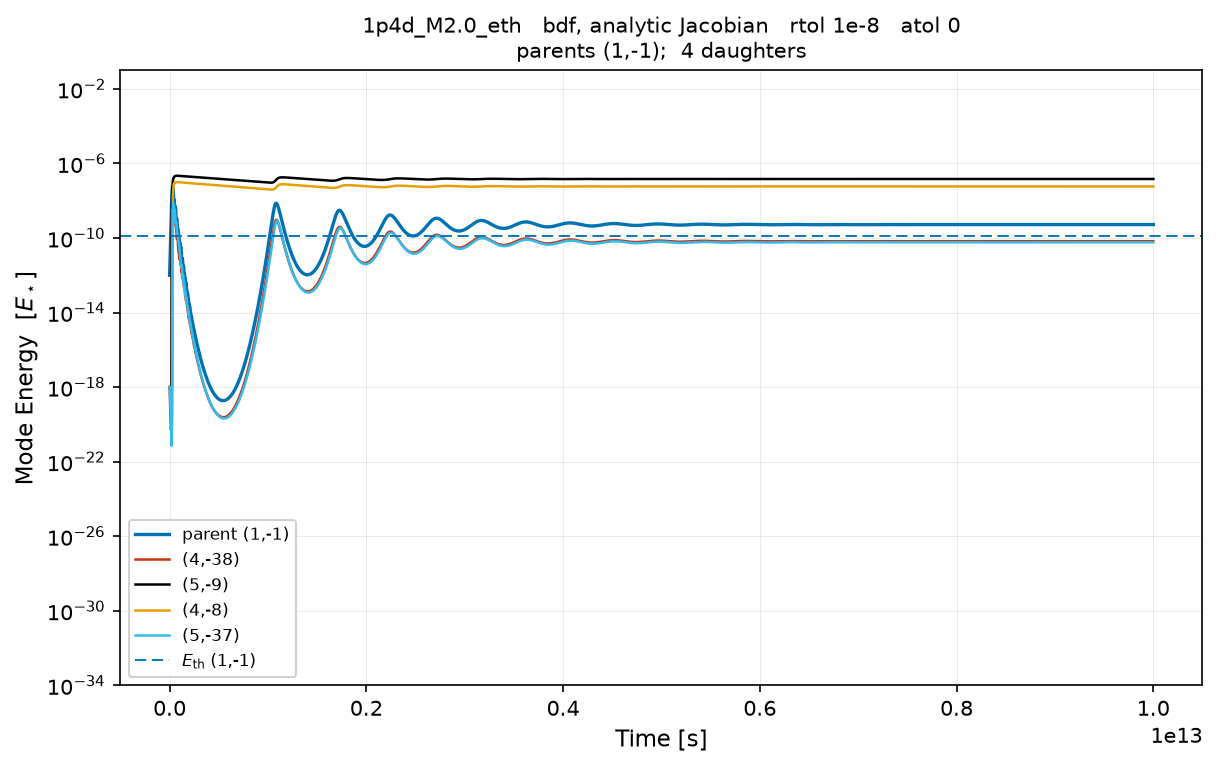
\includegraphics[width=0.21\textwidth,height=0.1323\textwidth]{../plots/bdf/1p4d_M2.0_eth/r1e-8_a0.png} \\[-1pt]
 & \parbox[t]{0.21\textwidth}{\centering\scriptsize 20.95\,M steps, 33.9\,s} & \parbox[t]{0.21\textwidth}{\centering\scriptsize 20.95\,M steps, 30.8\,s} & \parbox[t]{0.21\textwidth}{\centering\scriptsize 20.95\,M steps, 26.4\,s} & \parbox[t]{0.21\textwidth}{\centering\scriptsize 20.95\,M steps, 34.6\,s} \\[2pt]
\rotatebox{90}{\parbox{0.1323\textwidth}{\centering\scriptsize\bfseries BDF-Krylov, band full}} & 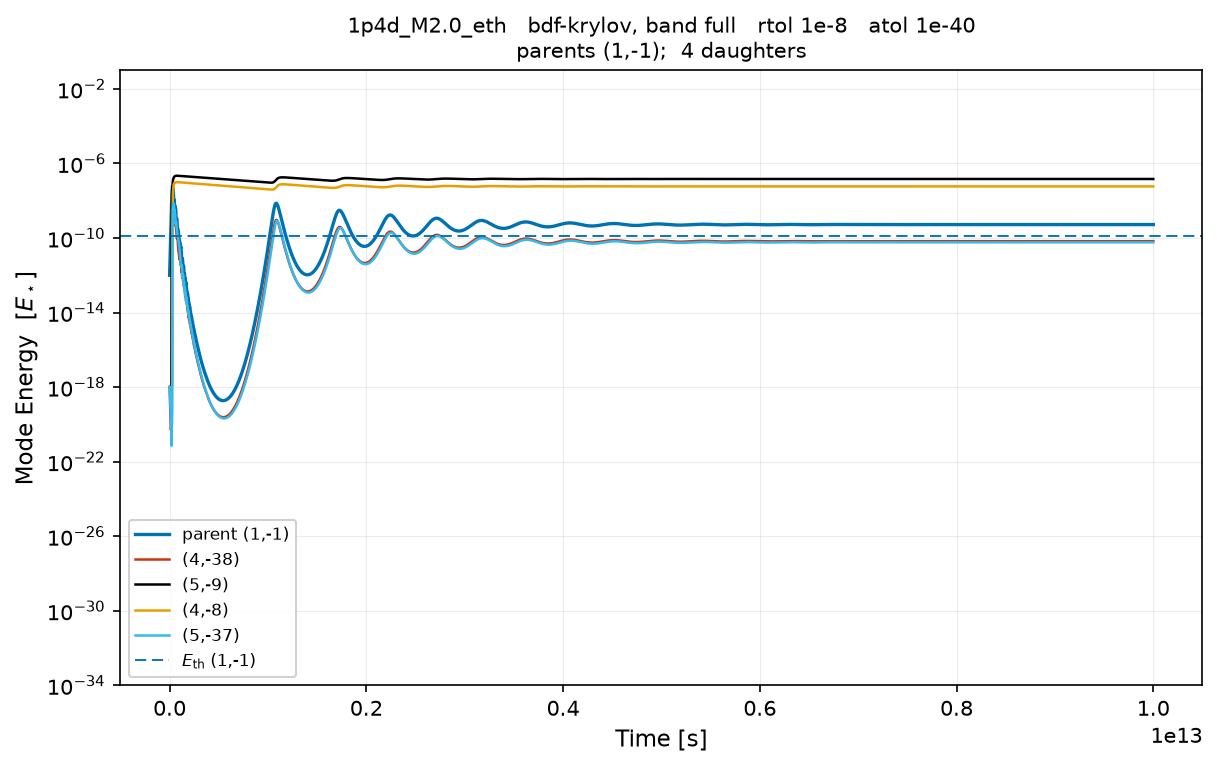
\includegraphics[width=0.21\textwidth,height=0.1323\textwidth]{../plots/krylov_full/1p4d_M2.0_eth/r1e-8_a1e-40.png} & 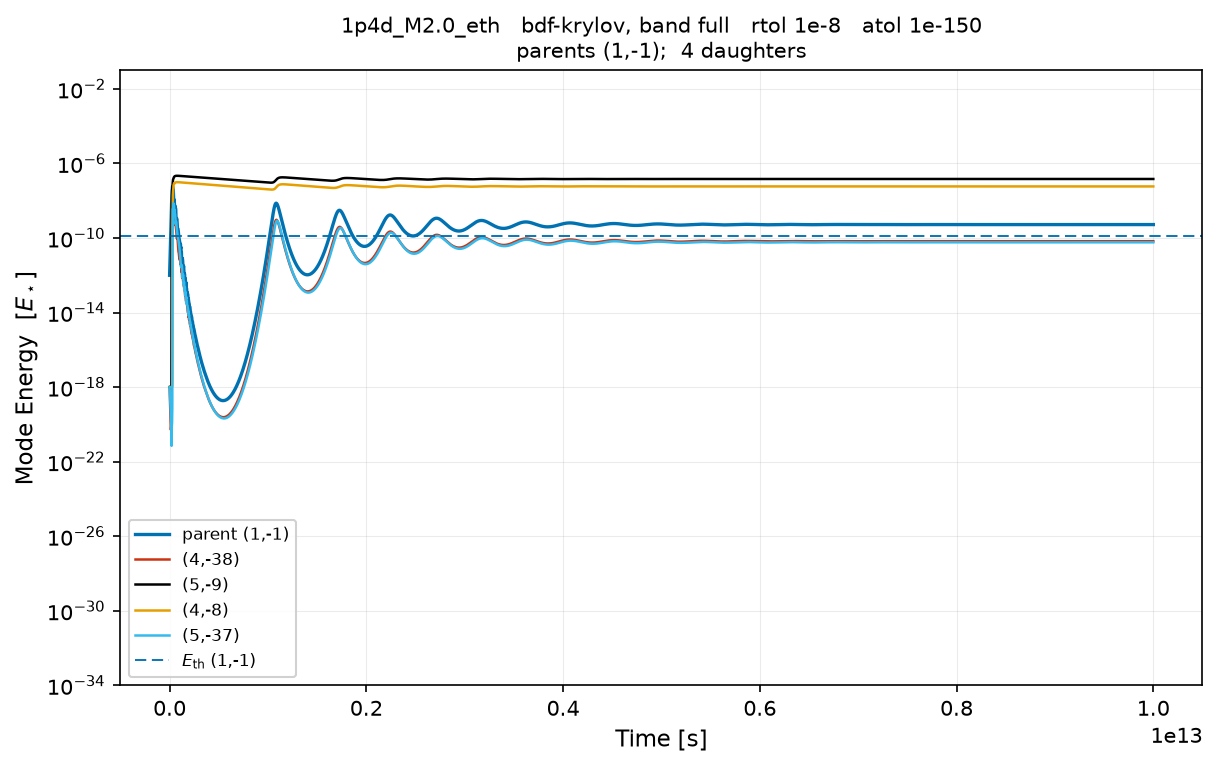
\includegraphics[width=0.21\textwidth,height=0.1323\textwidth]{../plots/krylov_full/1p4d_M2.0_eth/r1e-8_a1e-150.png} & 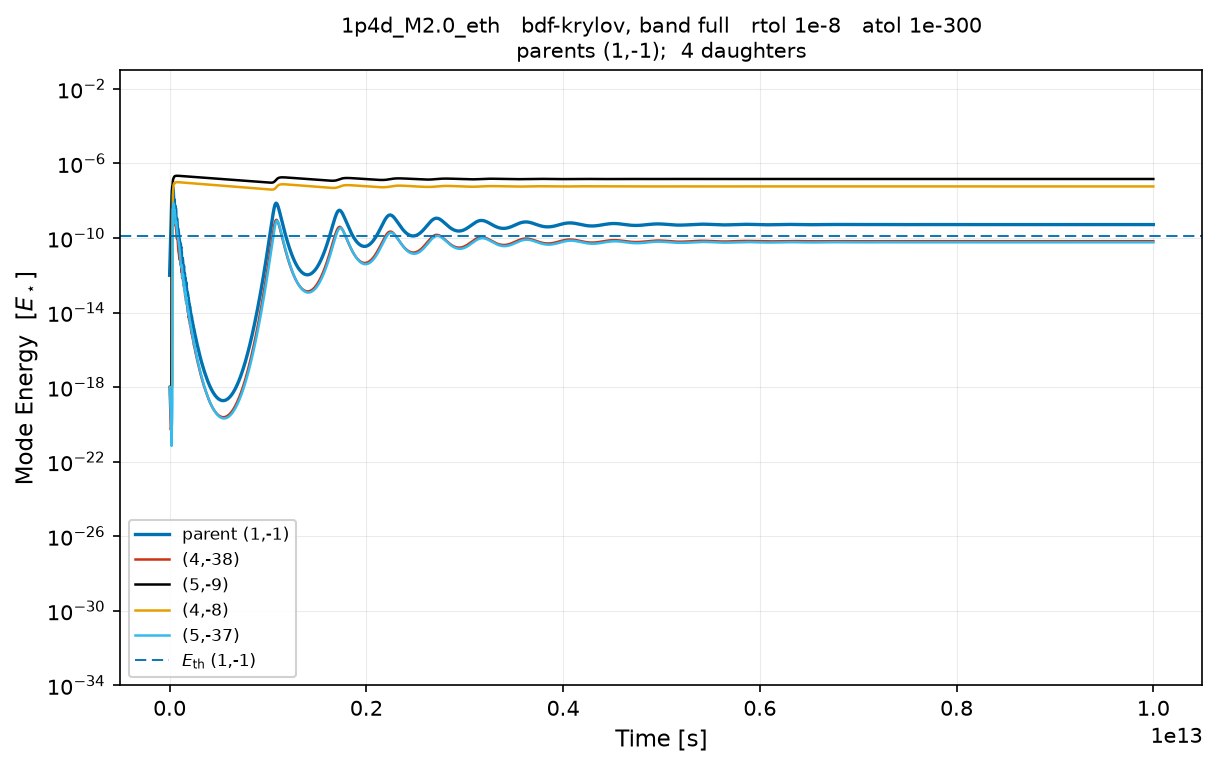
\includegraphics[width=0.21\textwidth,height=0.1323\textwidth]{../plots/krylov_full/1p4d_M2.0_eth/r1e-8_a1e-300.png} & 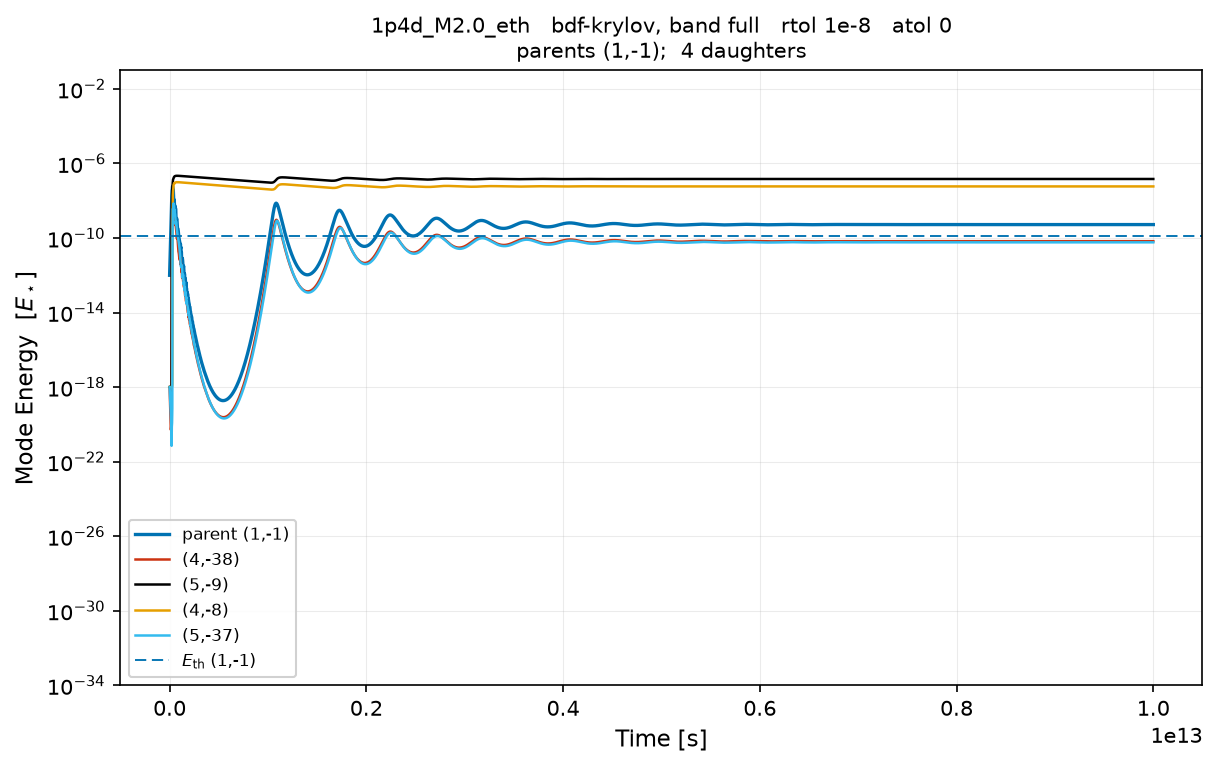
\includegraphics[width=0.21\textwidth,height=0.1323\textwidth]{../plots/krylov_full/1p4d_M2.0_eth/r1e-8_a0.png} \\[-1pt]
 & \parbox[t]{0.21\textwidth}{\centering\scriptsize 19.99\,M steps, 29.7\,s} & \parbox[t]{0.21\textwidth}{\centering\scriptsize 19.99\,M steps, 50.6\,s} & \parbox[t]{0.21\textwidth}{\centering\scriptsize 19.99\,M steps, 28.5\,s} & \parbox[t]{0.21\textwidth}{\centering\scriptsize 19.99\,M steps, 49.4\,s} \\[2pt]
\rotatebox{90}{\parbox{0.1323\textwidth}{\centering\scriptsize\bfseries BDF-Krylov, band 3}} & 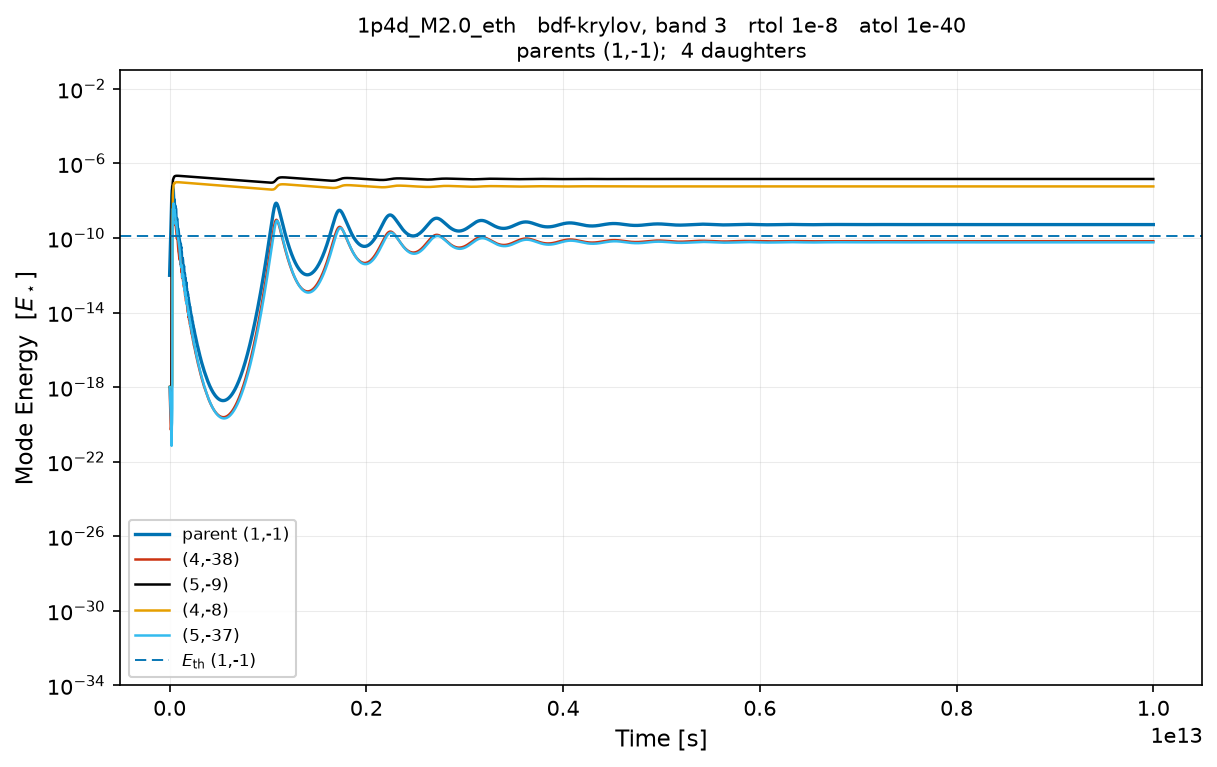
\includegraphics[width=0.21\textwidth,height=0.1323\textwidth]{../plots/krylov_b3/1p4d_M2.0_eth/r1e-8_a1e-40.png} & 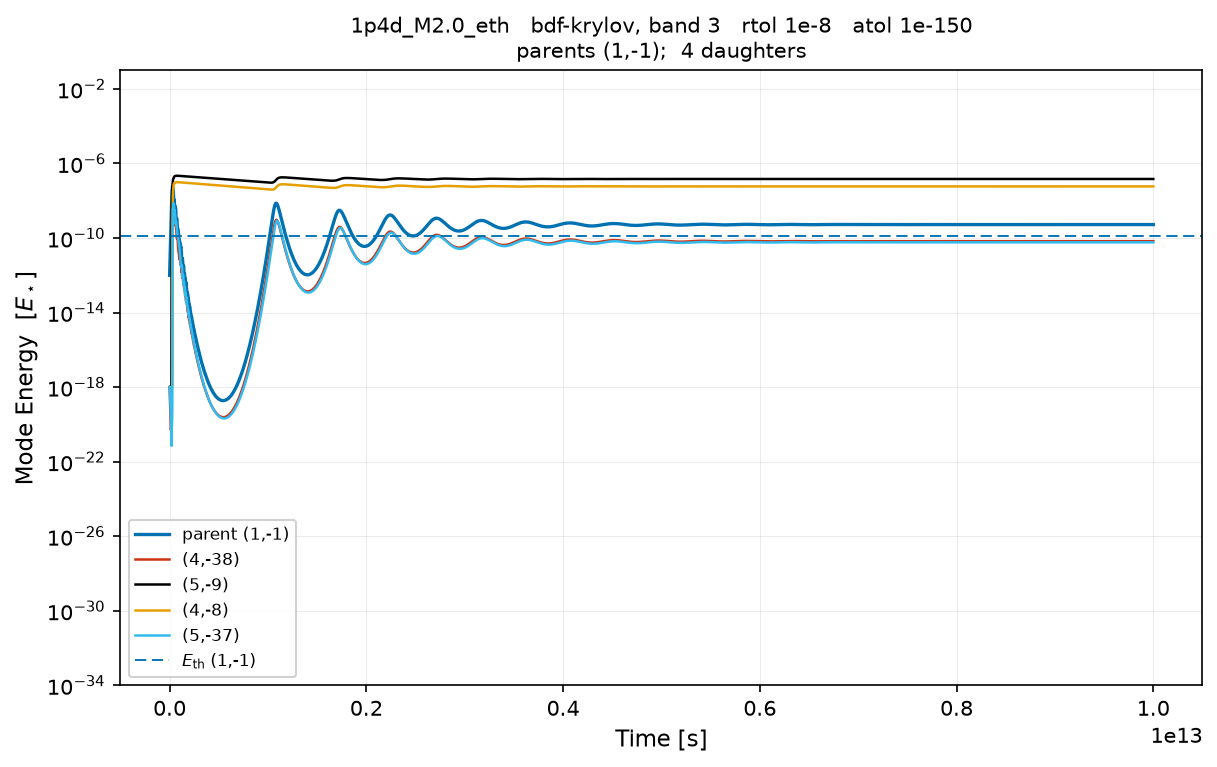
\includegraphics[width=0.21\textwidth,height=0.1323\textwidth]{../plots/krylov_b3/1p4d_M2.0_eth/r1e-8_a1e-150.png} & 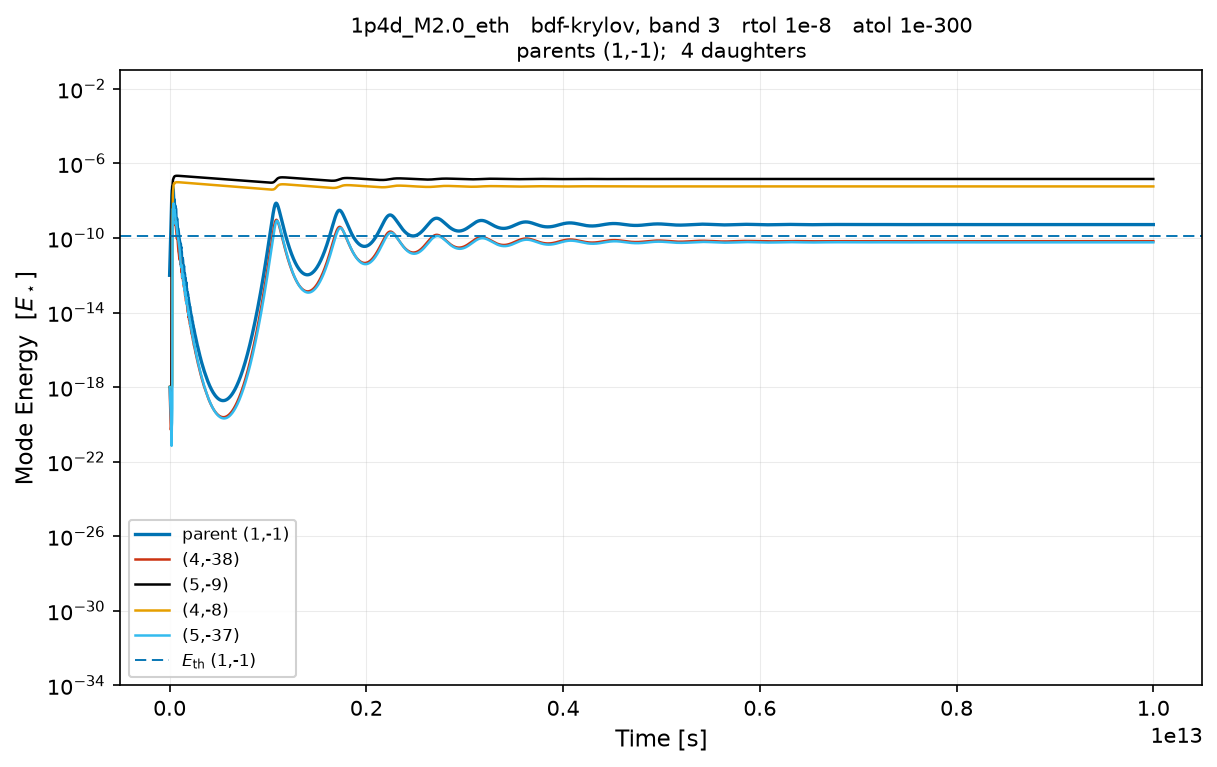
\includegraphics[width=0.21\textwidth,height=0.1323\textwidth]{../plots/krylov_b3/1p4d_M2.0_eth/r1e-8_a1e-300.png} & 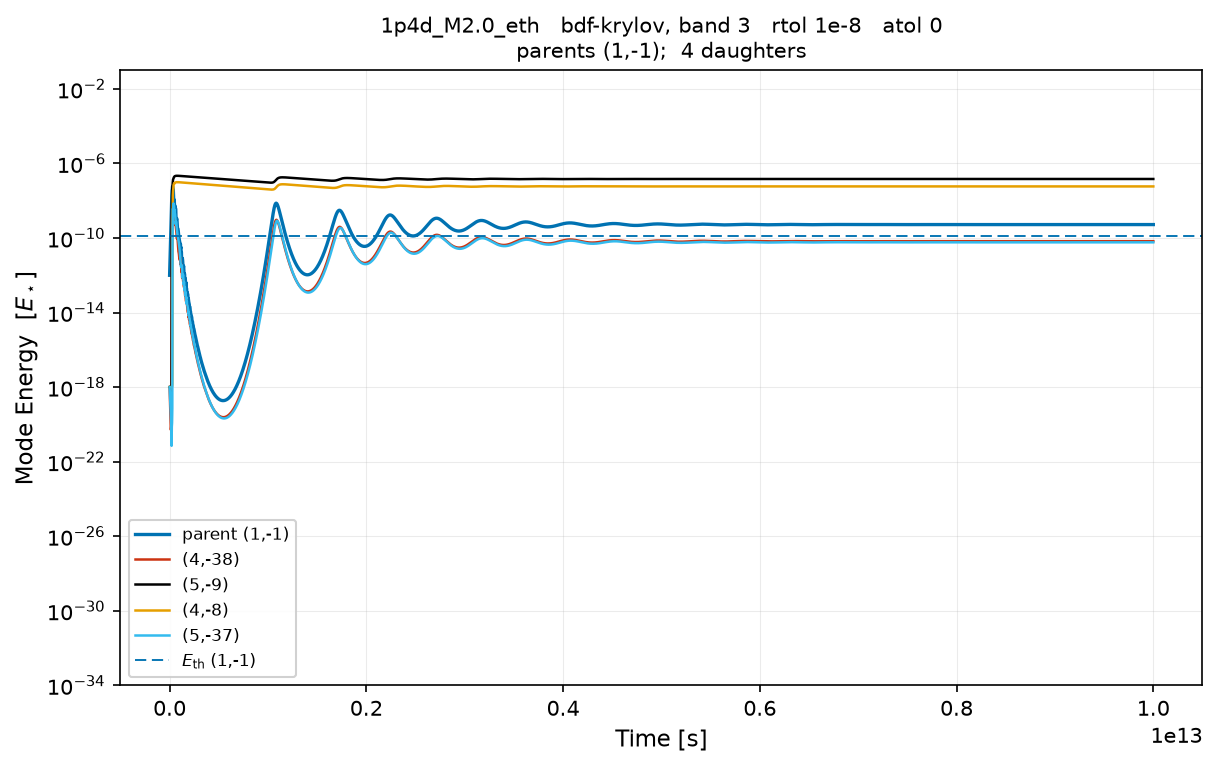
\includegraphics[width=0.21\textwidth,height=0.1323\textwidth]{../plots/krylov_b3/1p4d_M2.0_eth/r1e-8_a0.png} \\[-1pt]
 & \parbox[t]{0.21\textwidth}{\centering\scriptsize 19.90\,M steps, 30.2\,s} & \parbox[t]{0.21\textwidth}{\centering\scriptsize 19.89\,M steps, 50.7\,s} & \parbox[t]{0.21\textwidth}{\centering\scriptsize 19.89\,M steps, 35.2\,s} & \parbox[t]{0.21\textwidth}{\centering\scriptsize 19.89\,M steps, 36.8\,s} \\[2pt]
\rotatebox{90}{\parbox{0.1323\textwidth}{\centering\scriptsize\bfseries Adams, fixed point}} & 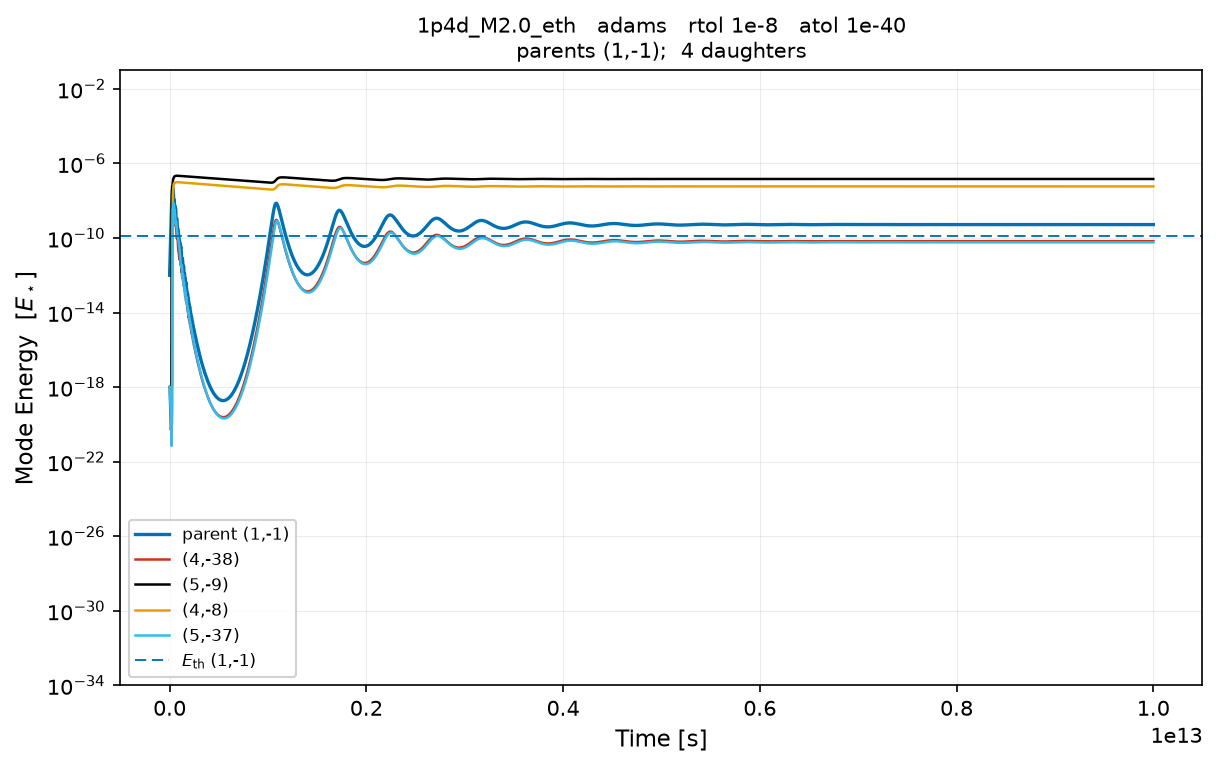
\includegraphics[width=0.21\textwidth,height=0.1323\textwidth]{../plots/adams/1p4d_M2.0_eth/r1e-8_a1e-40.png} & 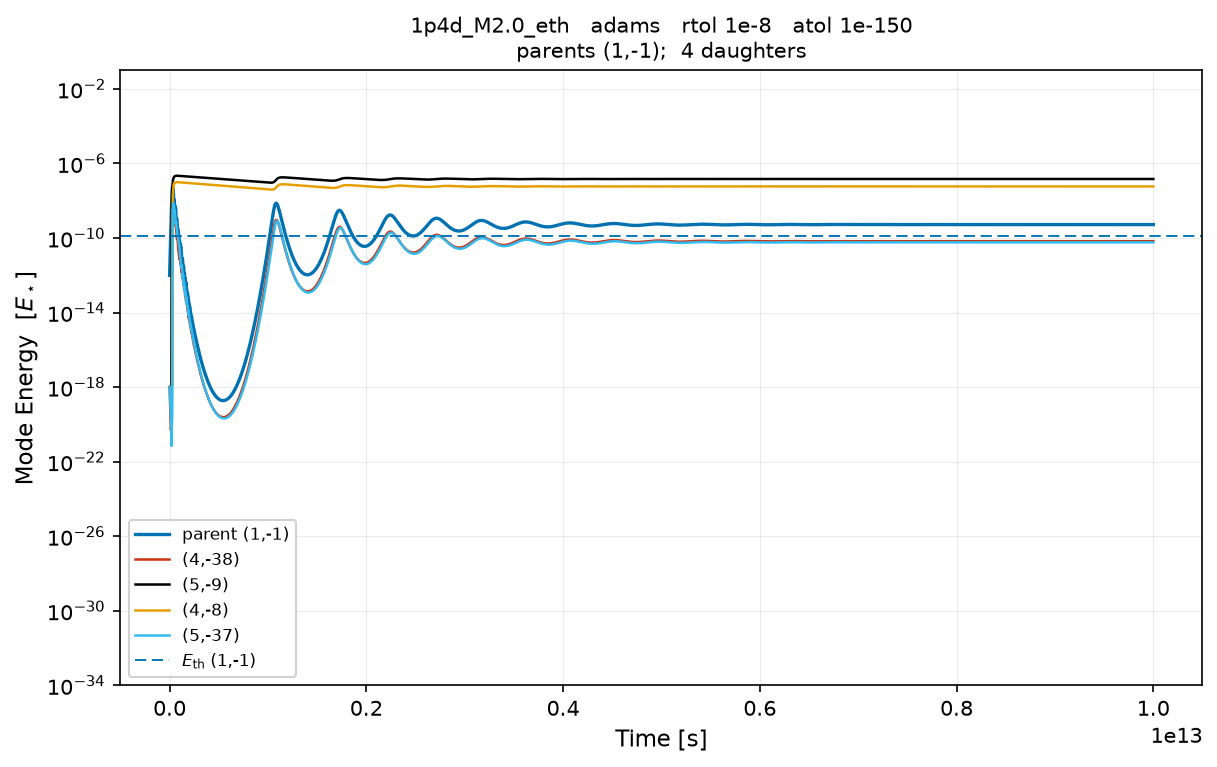
\includegraphics[width=0.21\textwidth,height=0.1323\textwidth]{../plots/adams/1p4d_M2.0_eth/r1e-8_a1e-150.png} & 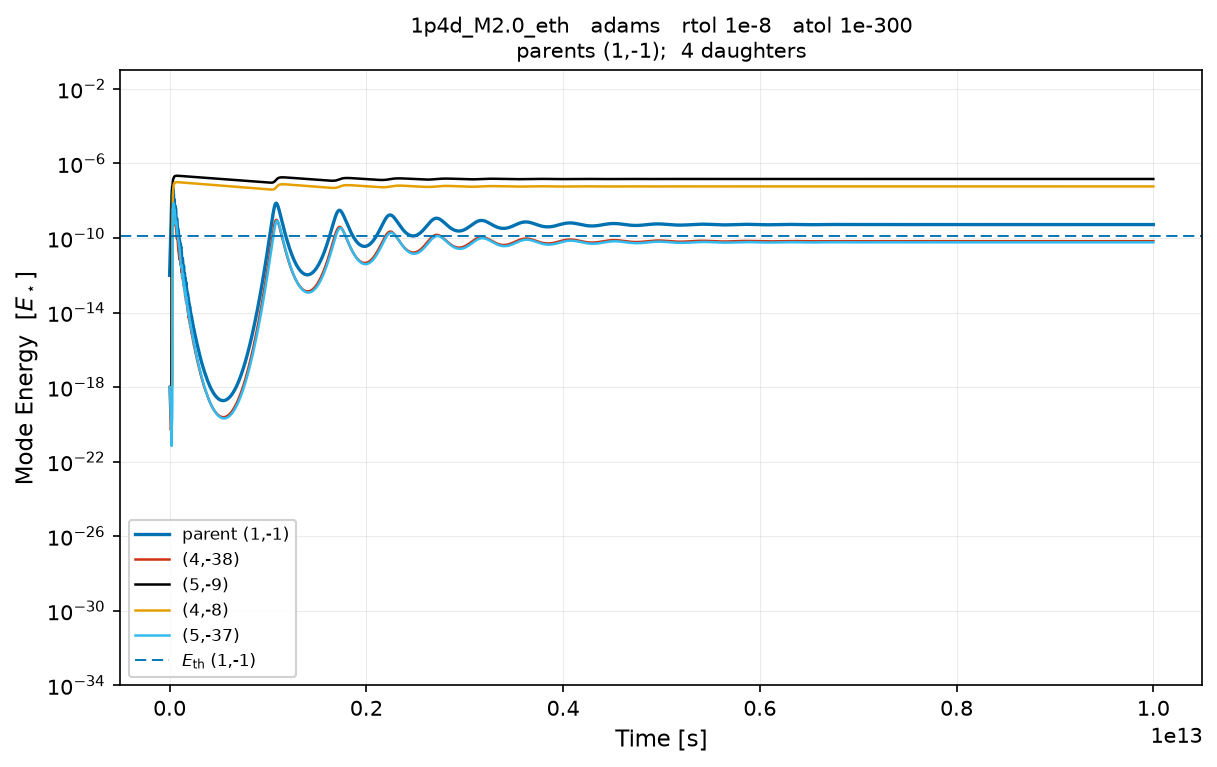
\includegraphics[width=0.21\textwidth,height=0.1323\textwidth]{../plots/adams/1p4d_M2.0_eth/r1e-8_a1e-300.png} & 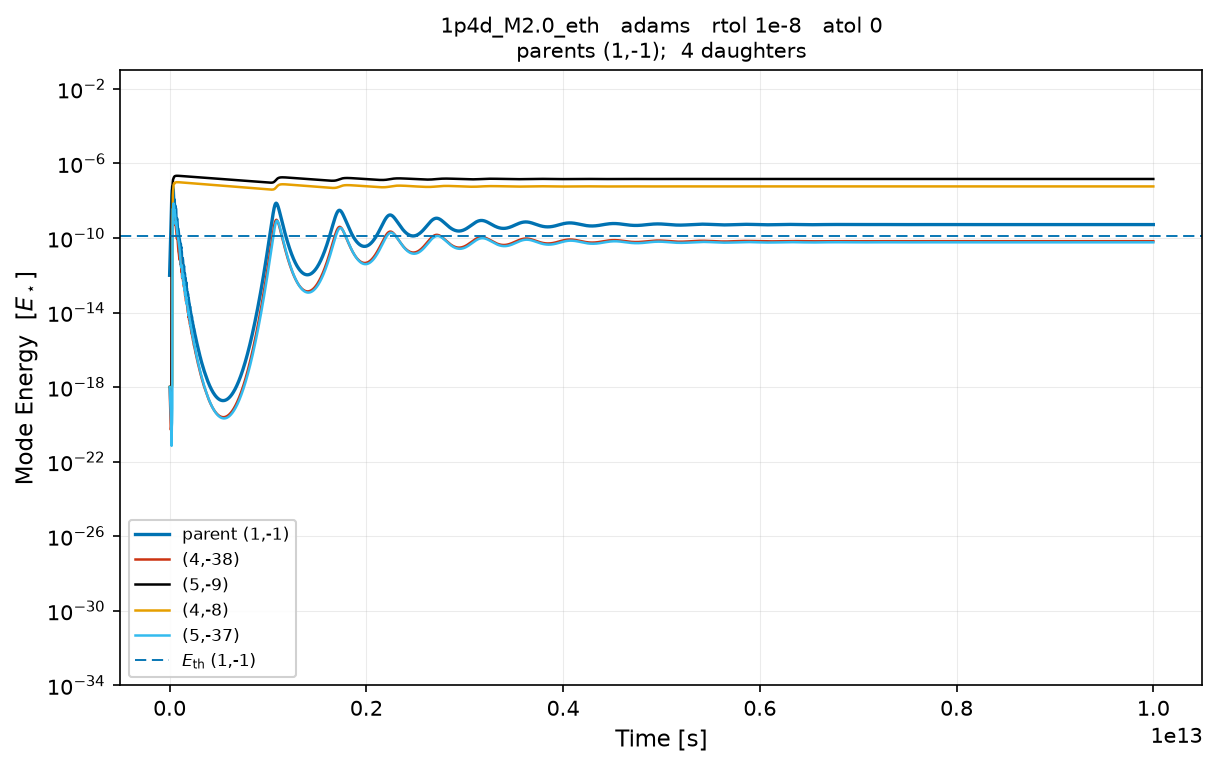
\includegraphics[width=0.21\textwidth,height=0.1323\textwidth]{../plots/adams/1p4d_M2.0_eth/r1e-8_a0.png} \\[-1pt]
 & \parbox[t]{0.21\textwidth}{\centering\scriptsize 12.04\,M steps, 18.8\,s} & \parbox[t]{0.21\textwidth}{\centering\scriptsize 12.04\,M steps, 15.4\,s} & \parbox[t]{0.21\textwidth}{\centering\scriptsize 12.04\,M steps, 18.5\,s} & \parbox[t]{0.21\textwidth}{\centering\scriptsize 12.04\,M steps, 11.4\,s} \\[2pt]
\end{tabular}\par}
\par\noindent{\scriptsize\setlength\tabcolsep{3.5pt}\renewcommand\arraystretch{0.92}
\begin{tabular}{@{}llllrrrrrrr@{}}
\toprule
integrator & atol & stop & $t_{\rm stop}$ [s] & steps & rejected & RHS & Jac. & NL it. & lin. it. & wall [s] \\
\midrule
rk8pd & $10^{-40}$ & end & $1.00\times10^{13}$ & 2.41\,M & 469.8\,k & 31.29\,M & -- & -- & -- & 5.2 \\
 & $10^{-150}$ & end & $1.00\times10^{13}$ & 2.41\,M & 469.8\,k & 31.29\,M & -- & -- & -- & 10.5 \\
 & $10^{-300}$ & end & $1.00\times10^{13}$ & 2.41\,M & 469.8\,k & 31.29\,M & -- & -- & -- & 7.6 \\
 & $0$ & end & $1.00\times10^{13}$ & 2.41\,M & 469.8\,k & 31.29\,M & -- & -- & -- & 10.1 \\
\addlinespace[2pt]
BDF, dense analytic Jacobian & $10^{-40}$ & end & $1.00\times10^{13}$ & 20.95\,M & 234.2\,k & 22.64\,M & 370.5\,k & 22.63\,M & -- & 33.9 \\
 & $10^{-150}$ & end & $1.00\times10^{13}$ & 20.95\,M & 234.2\,k & 22.64\,M & 370.5\,k & 22.63\,M & -- & 30.8 \\
 & $10^{-300}$ & end & $1.00\times10^{13}$ & 20.95\,M & 234.2\,k & 22.64\,M & 370.5\,k & 22.63\,M & -- & 26.4 \\
 & $0$ & end & $1.00\times10^{13}$ & 20.95\,M & 234.2\,k & 22.64\,M & 370.5\,k & 22.63\,M & -- & 34.6 \\
\addlinespace[2pt]
BDF-Krylov, band full & $10^{-40}$ & end & $1.00\times10^{13}$ & 19.99\,M & 229.1\,k & 47.20\,M & 345.1\,k & 21.71\,M & 22.04\,M & 29.7 \\
 & $10^{-150}$ & end & $1.00\times10^{13}$ & 19.99\,M & 229.1\,k & 47.20\,M & 345.1\,k & 21.71\,M & 22.04\,M & 50.6 \\
 & $10^{-300}$ & end & $1.00\times10^{13}$ & 19.99\,M & 229.1\,k & 47.20\,M & 345.1\,k & 21.71\,M & 22.04\,M & 28.5 \\
 & $0$ & end & $1.00\times10^{13}$ & 19.99\,M & 229.1\,k & 47.20\,M & 345.1\,k & 21.71\,M & 22.04\,M & 49.4 \\
\addlinespace[2pt]
BDF-Krylov, band 3 & $10^{-40}$ & end & $1.00\times10^{13}$ & 19.90\,M & 240.9\,k & 47.57\,M & 343.7\,k & 21.69\,M & 23.47\,M & 30.2 \\
 & $10^{-150}$ & end & $1.00\times10^{13}$ & 19.89\,M & 240.0\,k & 47.56\,M & 343.5\,k & 21.68\,M & 23.48\,M & 50.7 \\
 & $10^{-300}$ & end & $1.00\times10^{13}$ & 19.89\,M & 240.0\,k & 47.56\,M & 343.5\,k & 21.68\,M & 23.48\,M & 35.2 \\
 & $0$ & end & $1.00\times10^{13}$ & 19.89\,M & 240.0\,k & 47.56\,M & 343.5\,k & 21.68\,M & 23.48\,M & 36.8 \\
\addlinespace[2pt]
Adams, fixed point & $10^{-40}$ & end & $1.00\times10^{13}$ & 12.04\,M & 642.1\,k & 19.37\,M & -- & 19.36\,M & -- & 18.8 \\
 & $10^{-150}$ & end & $1.00\times10^{13}$ & 12.04\,M & 642.1\,k & 19.37\,M & -- & 19.36\,M & -- & 15.4 \\
 & $10^{-300}$ & end & $1.00\times10^{13}$ & 12.04\,M & 642.1\,k & 19.37\,M & -- & 19.36\,M & -- & 18.5 \\
 & $0$ & end & $1.00\times10^{13}$ & 12.04\,M & 642.1\,k & 19.37\,M & -- & 19.36\,M & -- & 11.4 \\
\bottomrule
\end{tabular}}

\clearpage
\subsection{\texttt{2p\_M1.7\_eth}}\label{net:2p_M1.7_eth}
\noindent\begin{minipage}[t]{0.43\textwidth}\vspace{0pt}\footnotesize
\begin{tabular}{@{}rrlrr@{}}
\toprule
id & gen & $(\ell,n)$ & $\omega$ [rad\,s$^{-1}$] & $\gamma$ [s$^{-1}$] \\
\midrule
0 & 0 & (1,+1) & $1.402\times10^{-3}$ & $-1.150\times10^{-10}$ \\
1 & 0 & (2,$-$3) & $8.582\times10^{-4}$ & $-3.458\times10^{-14}$ \\
2 & 1 & (6,$-$6) & $1.070\times10^{-3}$ & $4.184\times10^{-13}$ \\
3 & 1 & (7,$-$27) & $3.326\times10^{-4}$ & $8.612\times10^{-10}$ \\
4 & 1 & (6,$-$27) & $2.895\times10^{-4}$ & $8.836\times10^{-10}$ \\
5 & 1 & (8,$-$17) & $5.688\times10^{-4}$ & $3.001\times10^{-11}$ \\
\bottomrule
\end{tabular}
\end{minipage}\hfill
\begin{minipage}[t]{0.55\textwidth}\vspace{0pt}\footnotesize
\textbf{Model} \texttt{dsct\_M1.7\_T7750}, rule eth, $N=1$, cut 0.15,
closure 0.005; 6 modes, 2 triplet(s).\\[2pt]
\textbf{Selecting pairs}\\ (1,+1) $\to$ (6,$-$6) + (7,$-$27): $\Delta/\omega_a=-3.98\times10^{-5}$, $\kappa=+0.107$, $E_{\rm th}=9.22\times10^{-11}$, $E_{\rm eq}=1.23\times10^{-10}$\\
(2,$-$3) $\to$ (6,$-$27) + (8,$-$17): $\Delta/\omega_a=5.08\times10^{-5}$, $\kappa=+0.156$, $E_{\rm th}=3.75\times10^{-9}$, $E_{\rm eq}=3.75\times10^{-9}$\\[2pt]

\end{minipage}

\par\smallskip{\centering\begin{tabular}{@{}c@{\hspace{2pt}}c@{\hspace{2pt}}c@{\hspace{2pt}}c@{\hspace{2pt}}c@{}}
 & \small atol $10^{-40}$ & \small atol $10^{-150}$ & \small atol $10^{-300}$ & \small atol $0$ \\[1pt]
\rotatebox{90}{\parbox{0.1323\textwidth}{\centering\scriptsize\bfseries rk8pd}} & 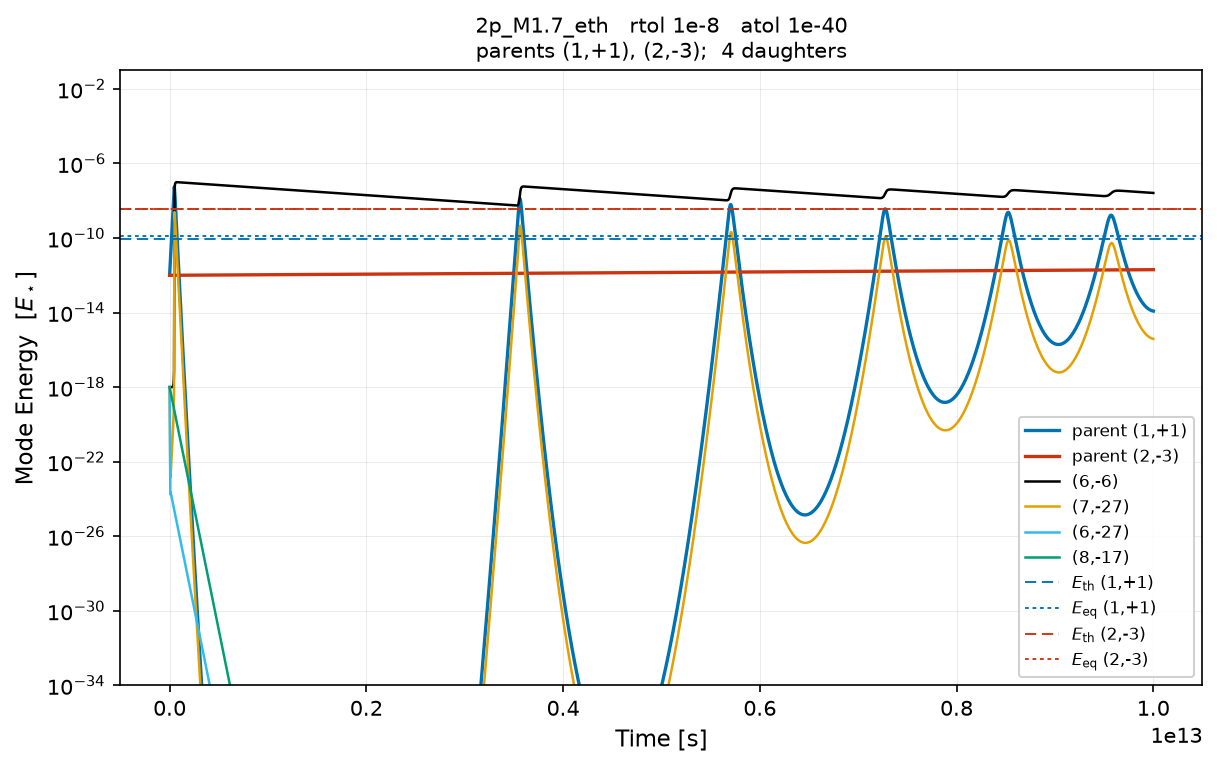
\includegraphics[width=0.21\textwidth,height=0.1323\textwidth]{../plots/rk8pd/2p_M1.7_eth/r1e-8_a1e-40.png} & 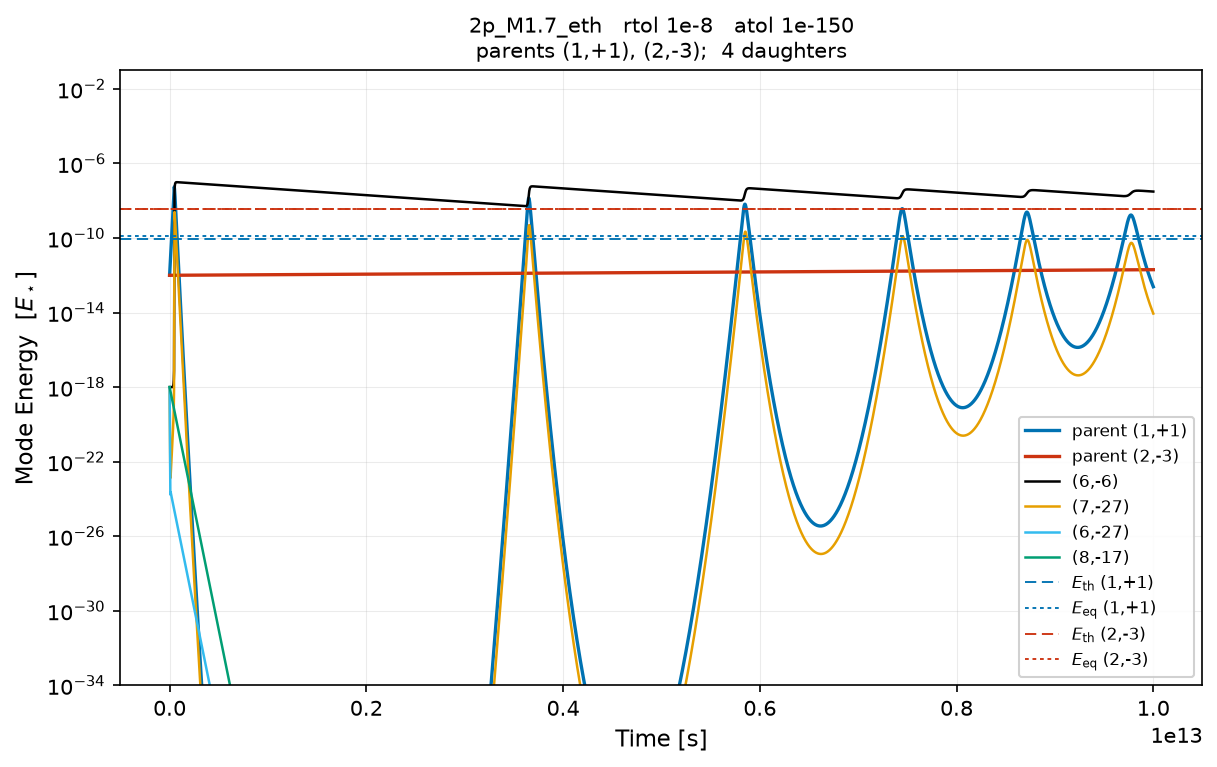
\includegraphics[width=0.21\textwidth,height=0.1323\textwidth]{../plots/rk8pd/2p_M1.7_eth/r1e-8_a1e-150.png} & 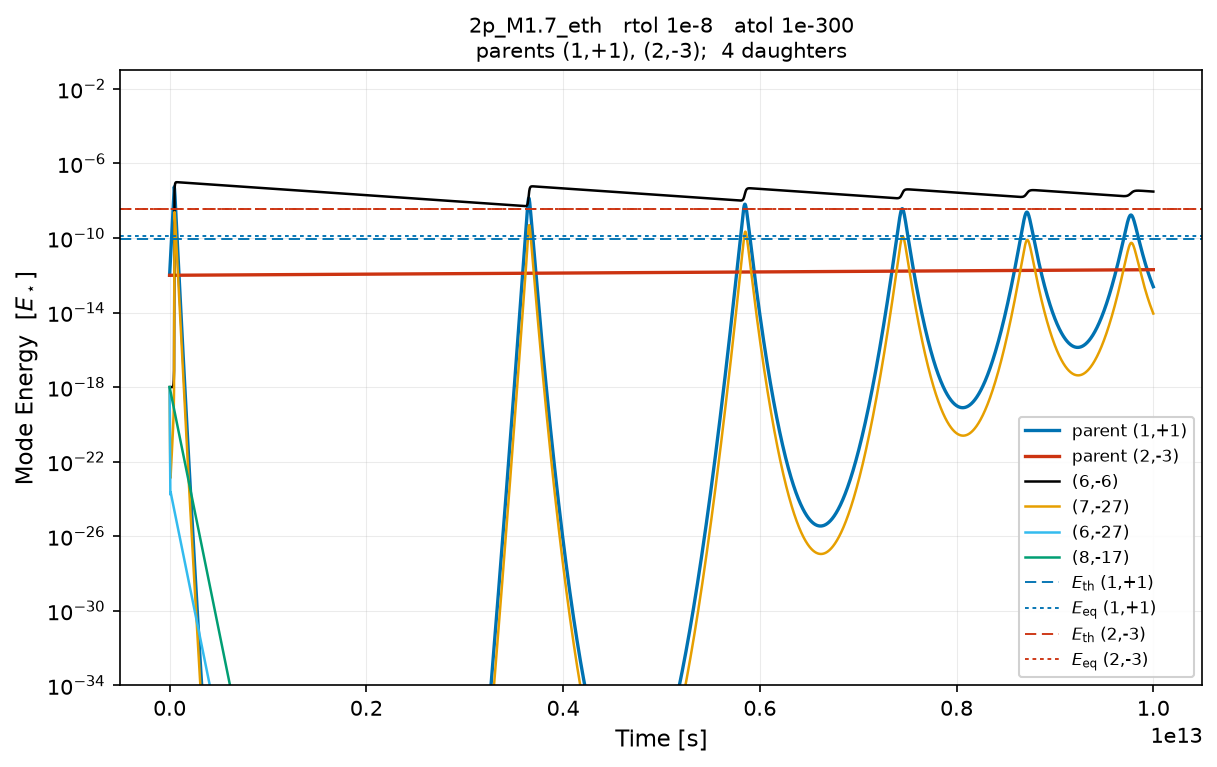
\includegraphics[width=0.21\textwidth,height=0.1323\textwidth]{../plots/rk8pd/2p_M1.7_eth/r1e-8_a1e-300.png} & 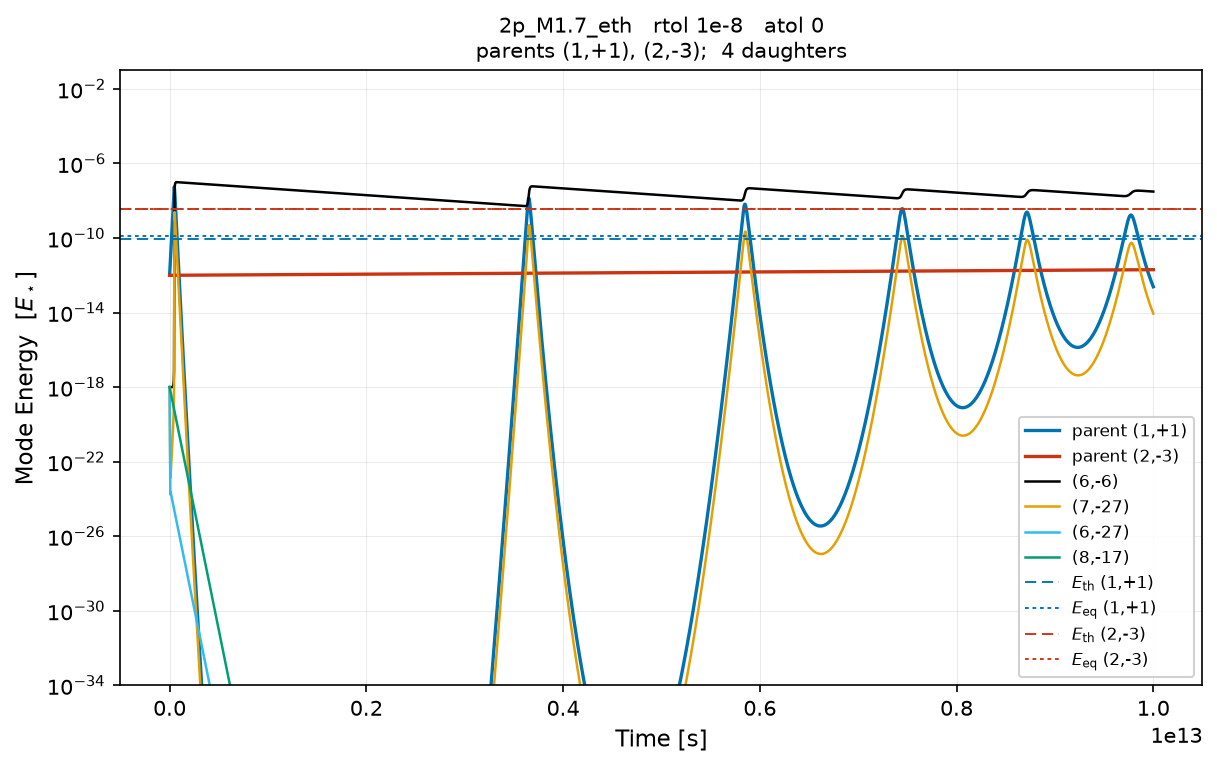
\includegraphics[width=0.21\textwidth,height=0.1323\textwidth]{../plots/rk8pd/2p_M1.7_eth/r1e-8_a0.png} \\[-1pt]
 & \parbox[t]{0.21\textwidth}{\centering\scriptsize 990.0\,k steps, 1.9\,s} & \parbox[t]{0.21\textwidth}{\centering\scriptsize 1.13\,M steps, 5.3\,s} & \parbox[t]{0.21\textwidth}{\centering\scriptsize 1.13\,M steps, 3.3\,s} & \parbox[t]{0.21\textwidth}{\centering\scriptsize 1.13\,M steps, 5.3\,s} \\[2pt]
\rotatebox{90}{\parbox{0.1323\textwidth}{\centering\scriptsize\bfseries BDF, dense analytic Jacobian}} & 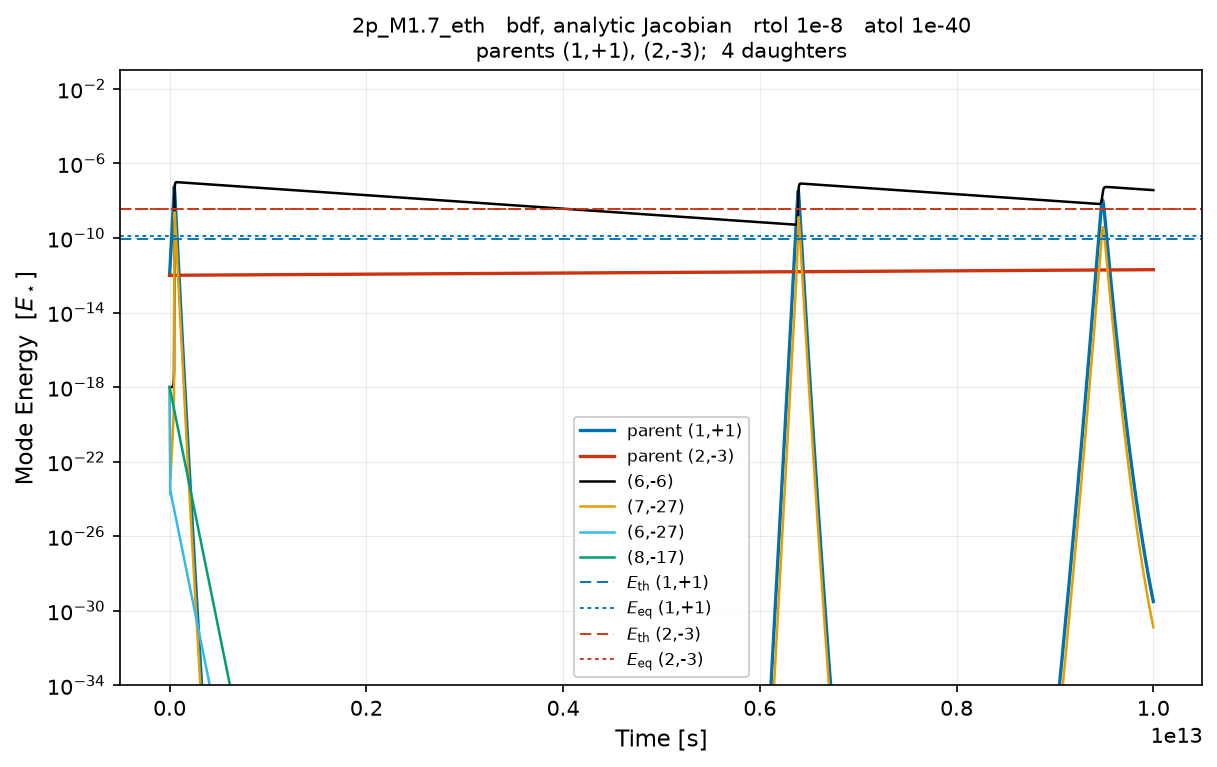
\includegraphics[width=0.21\textwidth,height=0.1323\textwidth]{../plots/bdf/2p_M1.7_eth/r1e-8_a1e-40.png} & 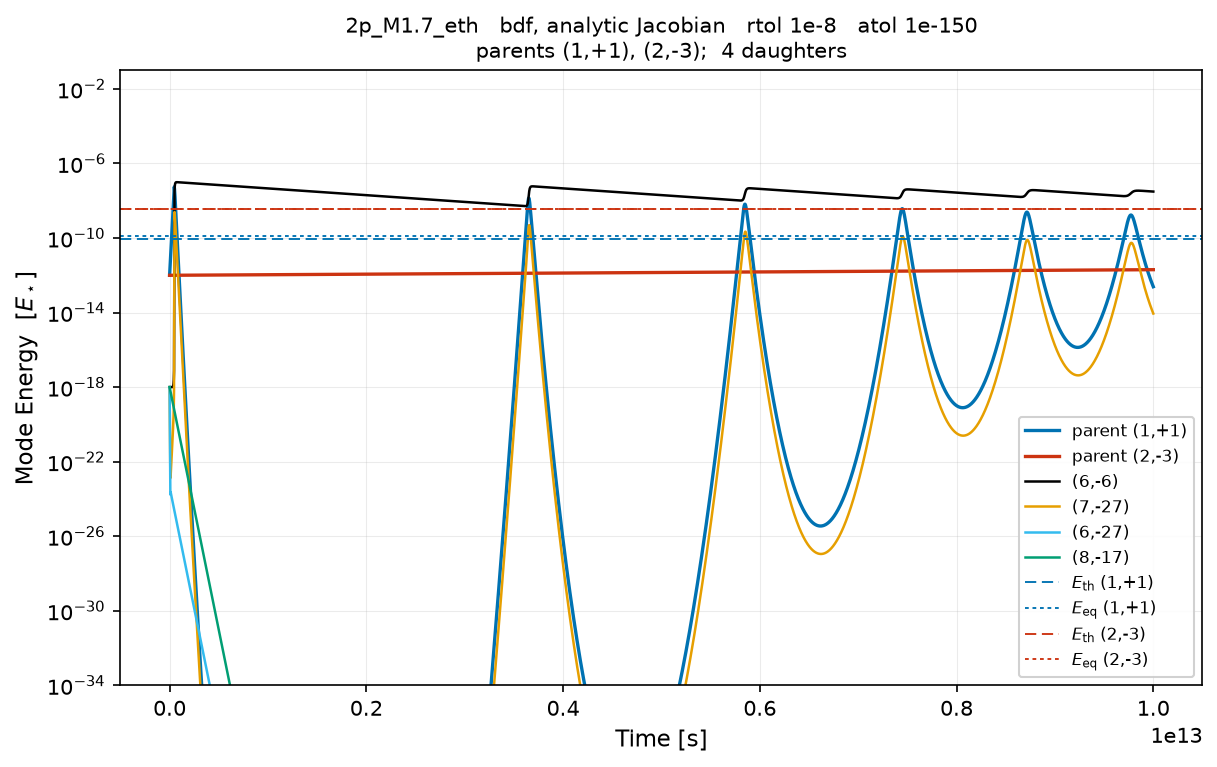
\includegraphics[width=0.21\textwidth,height=0.1323\textwidth]{../plots/bdf/2p_M1.7_eth/r1e-8_a1e-150.png} & 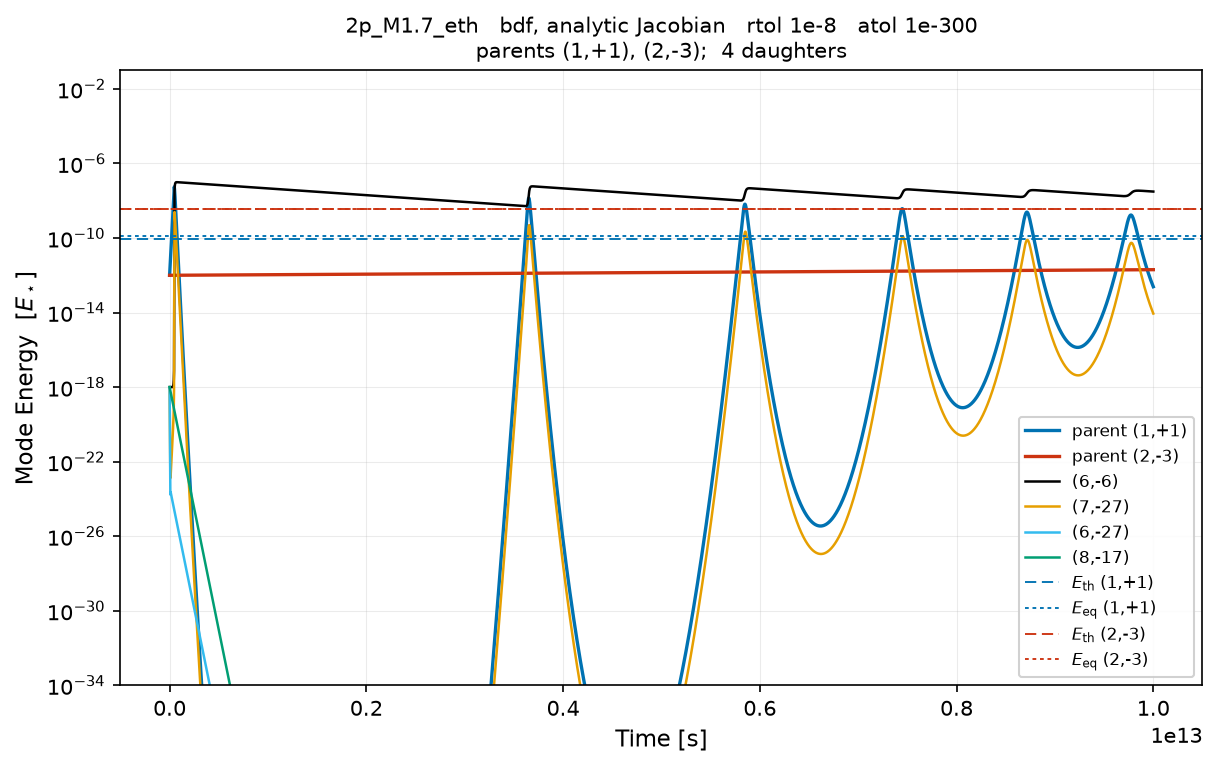
\includegraphics[width=0.21\textwidth,height=0.1323\textwidth]{../plots/bdf/2p_M1.7_eth/r1e-8_a1e-300.png} & 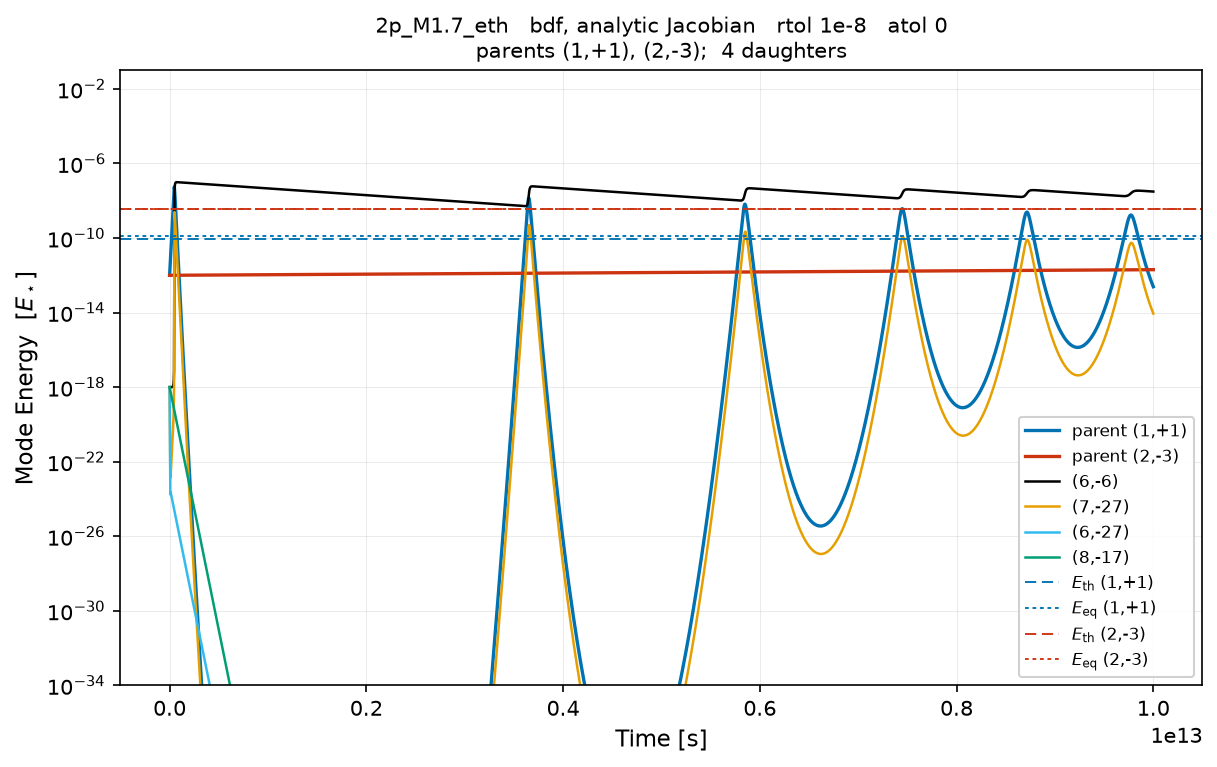
\includegraphics[width=0.21\textwidth,height=0.1323\textwidth]{../plots/bdf/2p_M1.7_eth/r1e-8_a0.png} \\[-1pt]
 & \parbox[t]{0.21\textwidth}{\centering\scriptsize 6.79\,M steps, 8.6\,s} & \parbox[t]{0.21\textwidth}{\centering\scriptsize 13.11\,M steps, 24.6\,s} & \parbox[t]{0.21\textwidth}{\centering\scriptsize 13.10\,M steps, 18.9\,s} & \parbox[t]{0.21\textwidth}{\centering\scriptsize 13.10\,M steps, 21.0\,s} \\[2pt]
\rotatebox{90}{\parbox{0.1323\textwidth}{\centering\scriptsize\bfseries BDF-Krylov, band full}} & 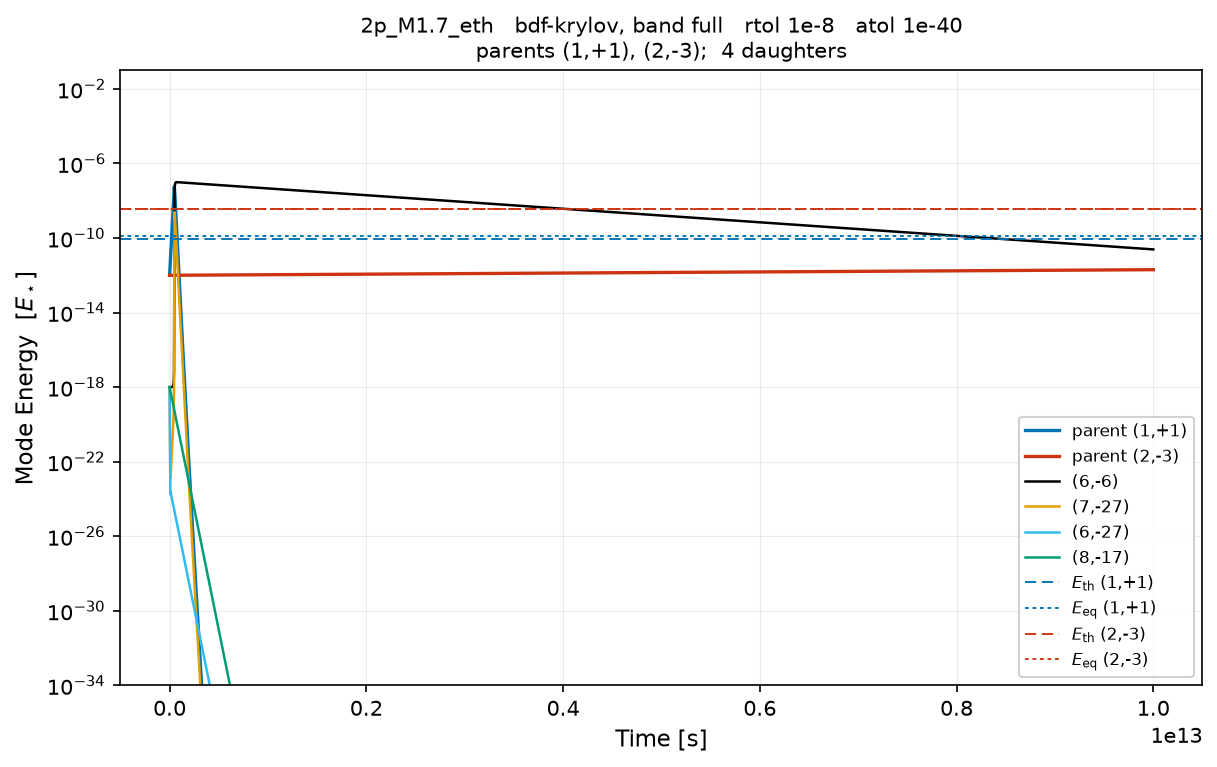
\includegraphics[width=0.21\textwidth,height=0.1323\textwidth]{../plots/krylov_full/2p_M1.7_eth/r1e-8_a1e-40.png} & 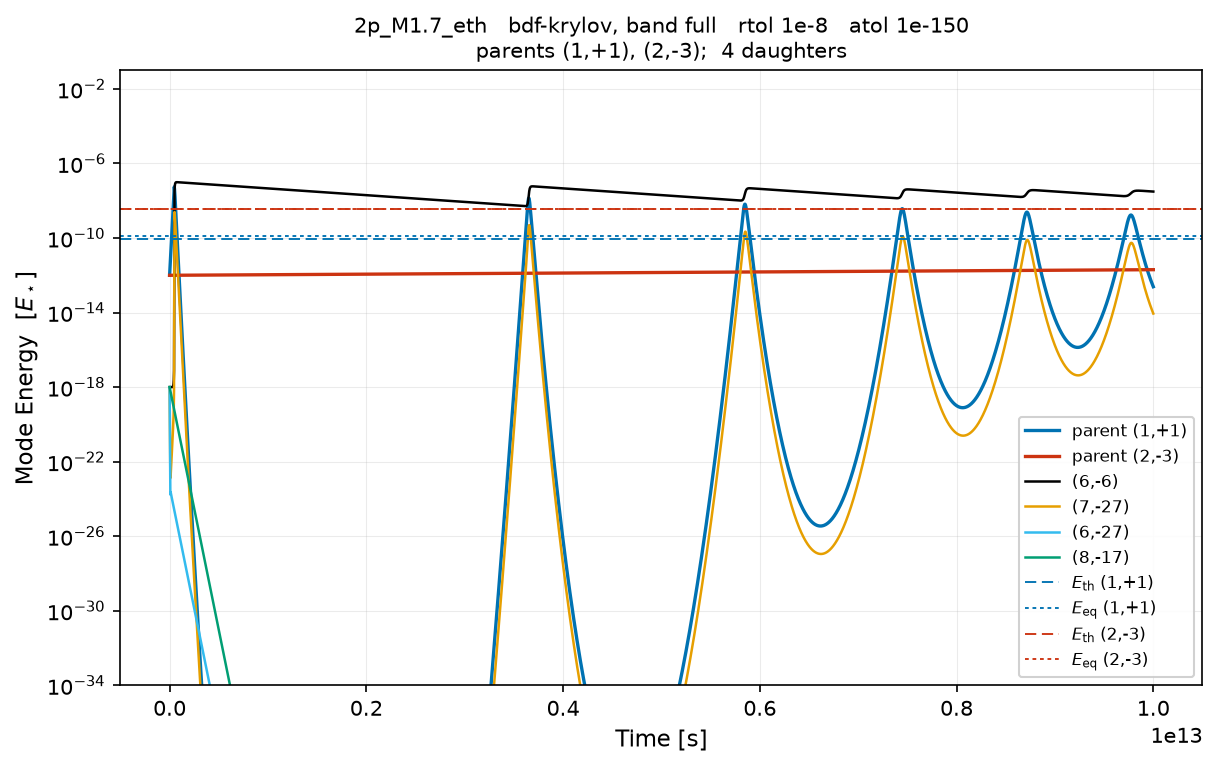
\includegraphics[width=0.21\textwidth,height=0.1323\textwidth]{../plots/krylov_full/2p_M1.7_eth/r1e-8_a1e-150.png} & 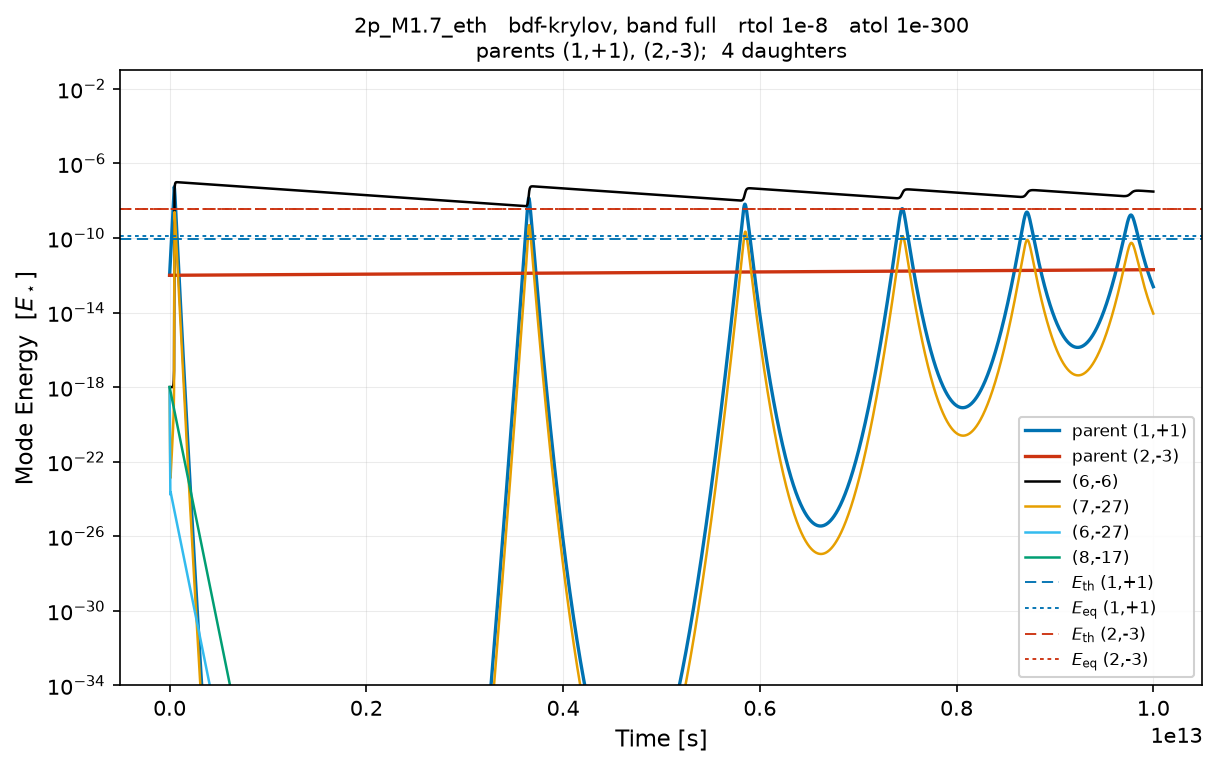
\includegraphics[width=0.21\textwidth,height=0.1323\textwidth]{../plots/krylov_full/2p_M1.7_eth/r1e-8_a1e-300.png} & 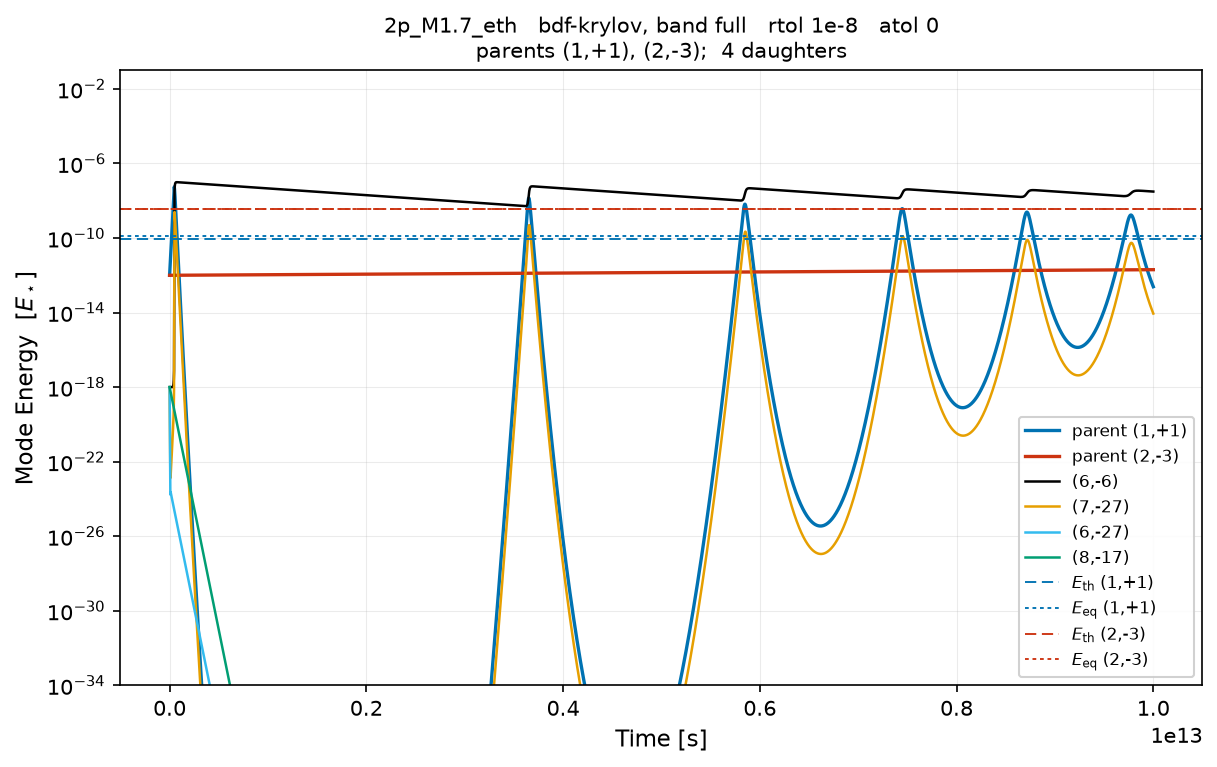
\includegraphics[width=0.21\textwidth,height=0.1323\textwidth]{../plots/krylov_full/2p_M1.7_eth/r1e-8_a0.png} \\[-1pt]
 & \parbox[t]{0.21\textwidth}{\centering\scriptsize 1.98\,M steps, 3.2\,s} & \parbox[t]{0.21\textwidth}{\centering\scriptsize 12.77\,M steps, 33.2\,s} & \parbox[t]{0.21\textwidth}{\centering\scriptsize 12.78\,M steps, 19.5\,s} & \parbox[t]{0.21\textwidth}{\centering\scriptsize 12.78\,M steps, 37.6\,s} \\[2pt]
\rotatebox{90}{\parbox{0.1323\textwidth}{\centering\scriptsize\bfseries BDF-Krylov, band 3}} & 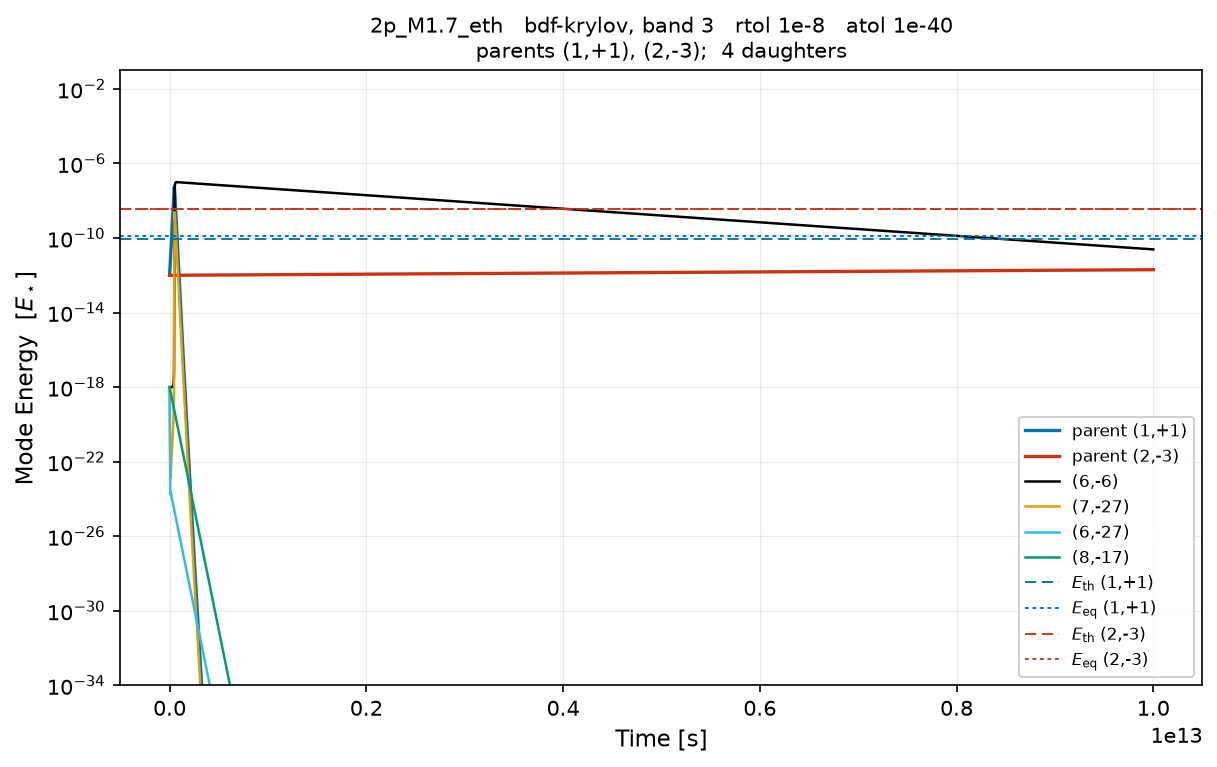
\includegraphics[width=0.21\textwidth,height=0.1323\textwidth]{../plots/krylov_b3/2p_M1.7_eth/r1e-8_a1e-40.png} & 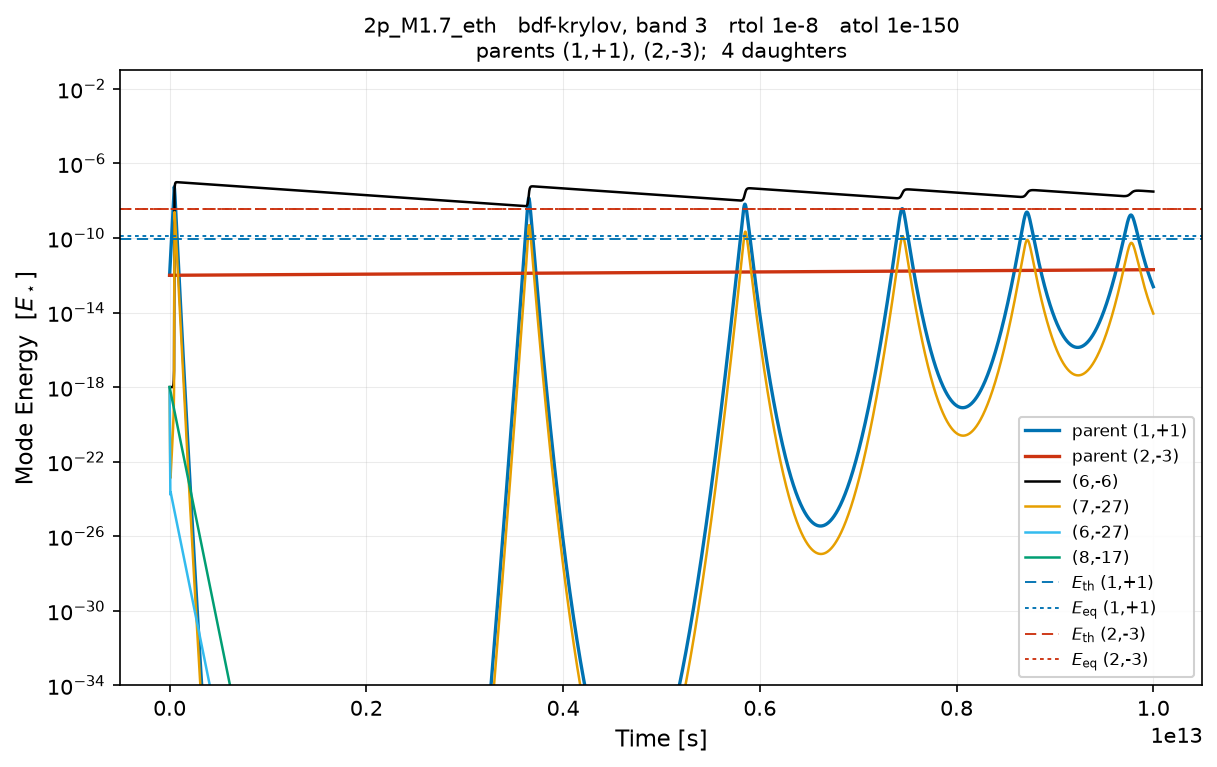
\includegraphics[width=0.21\textwidth,height=0.1323\textwidth]{../plots/krylov_b3/2p_M1.7_eth/r1e-8_a1e-150.png} & 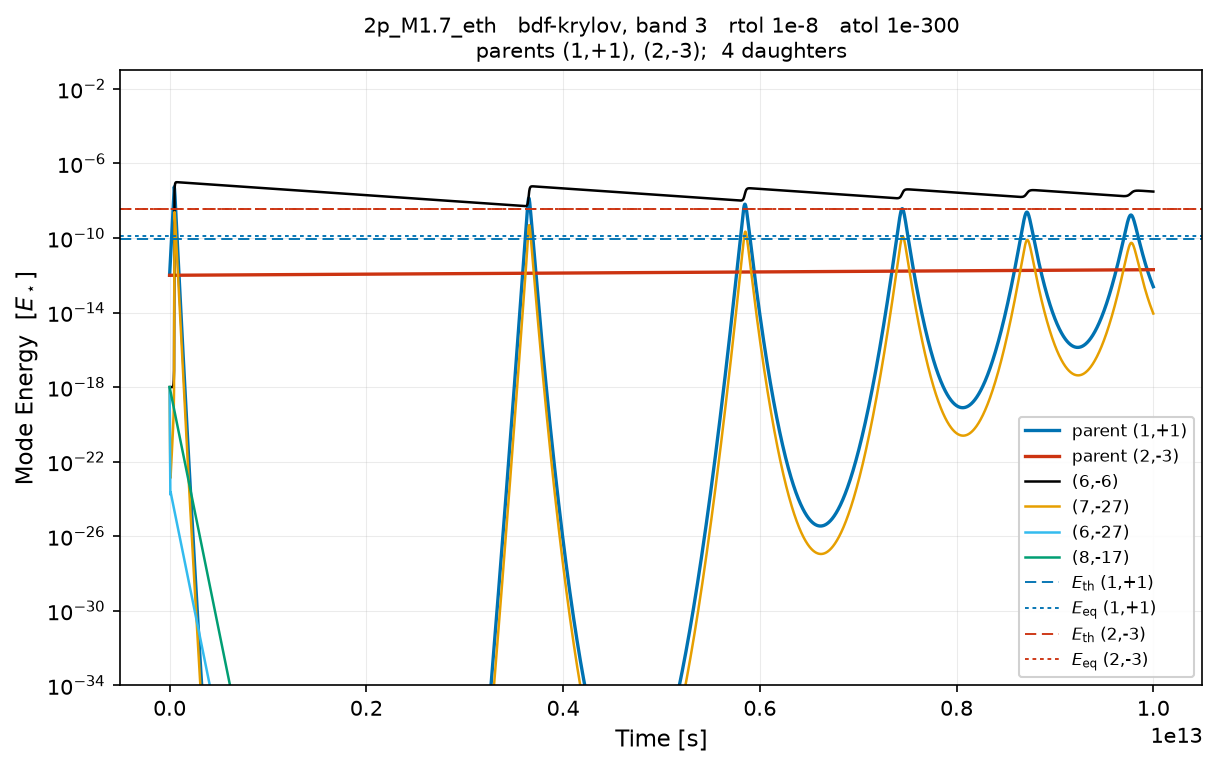
\includegraphics[width=0.21\textwidth,height=0.1323\textwidth]{../plots/krylov_b3/2p_M1.7_eth/r1e-8_a1e-300.png} & 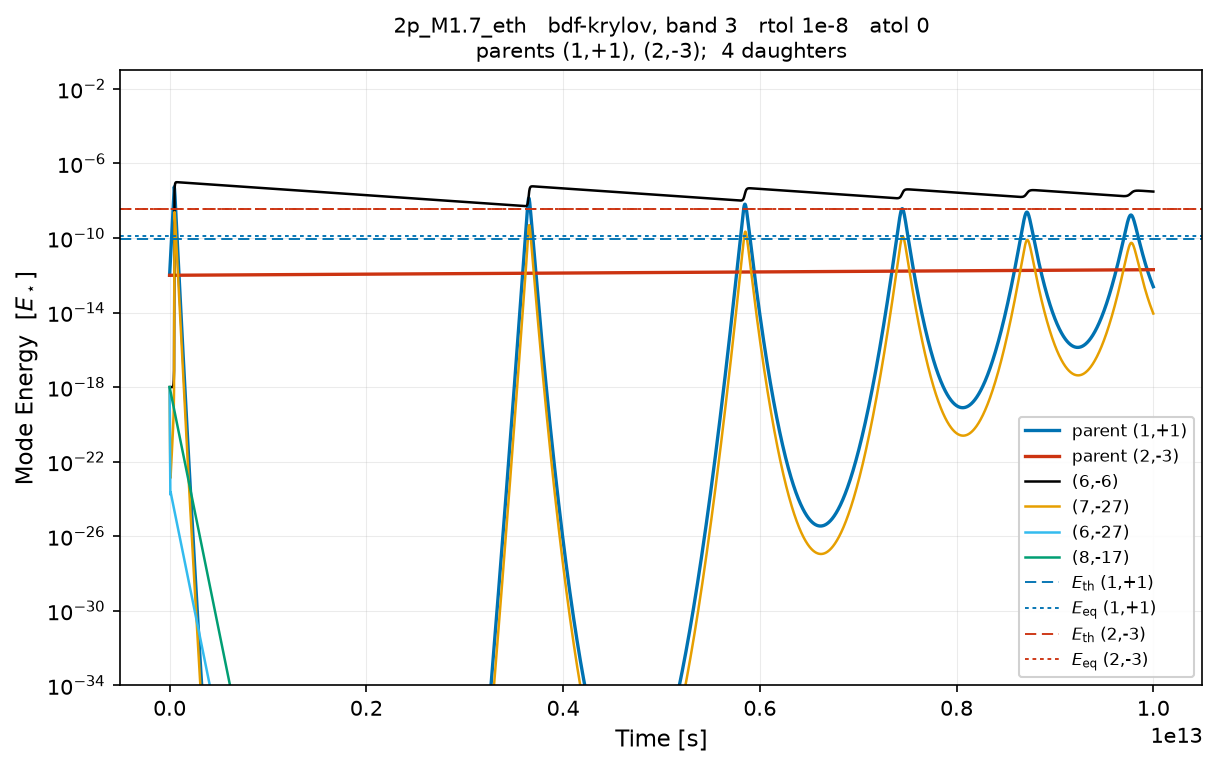
\includegraphics[width=0.21\textwidth,height=0.1323\textwidth]{../plots/krylov_b3/2p_M1.7_eth/r1e-8_a0.png} \\[-1pt]
 & \parbox[t]{0.21\textwidth}{\centering\scriptsize 2.19\,M steps, 6.3\,s} & \parbox[t]{0.21\textwidth}{\centering\scriptsize 12.40\,M steps, 38.2\,s} & \parbox[t]{0.21\textwidth}{\centering\scriptsize 12.41\,M steps, 27.7\,s} & \parbox[t]{0.21\textwidth}{\centering\scriptsize 12.41\,M steps, 24.7\,s} \\[2pt]
\rotatebox{90}{\parbox{0.1323\textwidth}{\centering\scriptsize\bfseries Adams, fixed point}} & 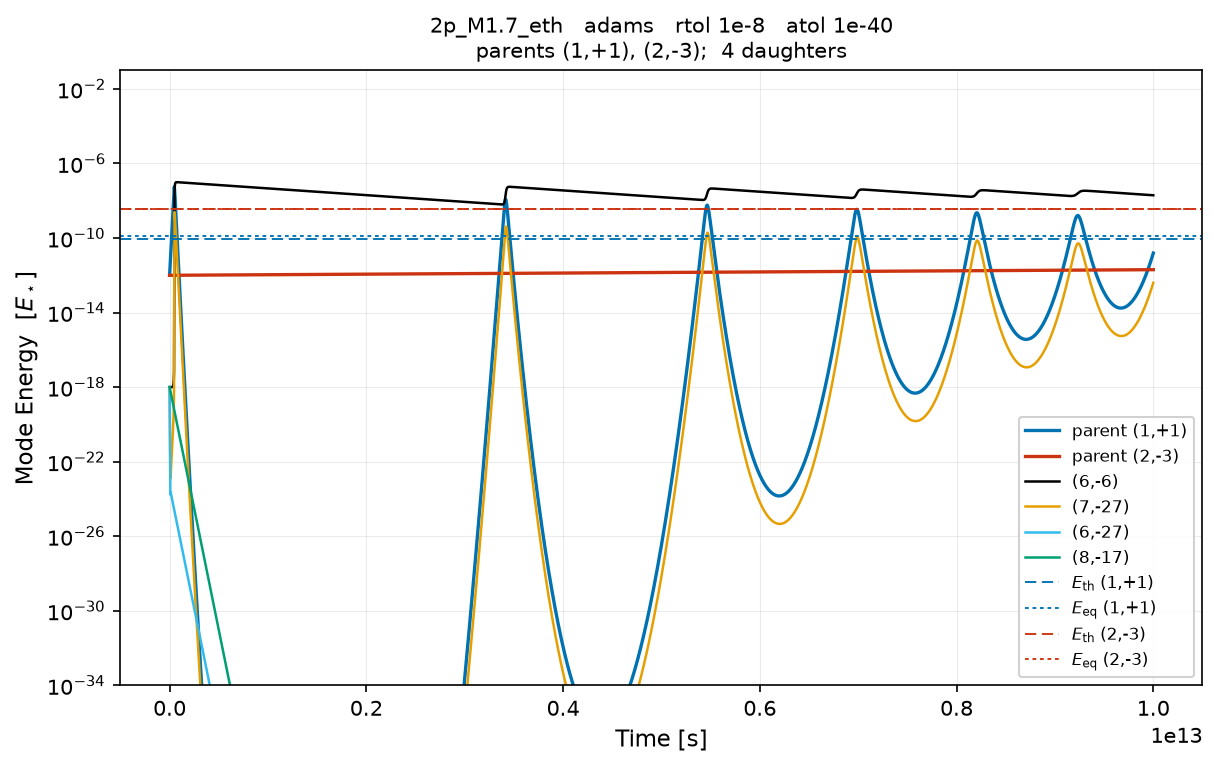
\includegraphics[width=0.21\textwidth,height=0.1323\textwidth]{../plots/adams/2p_M1.7_eth/r1e-8_a1e-40.png} & 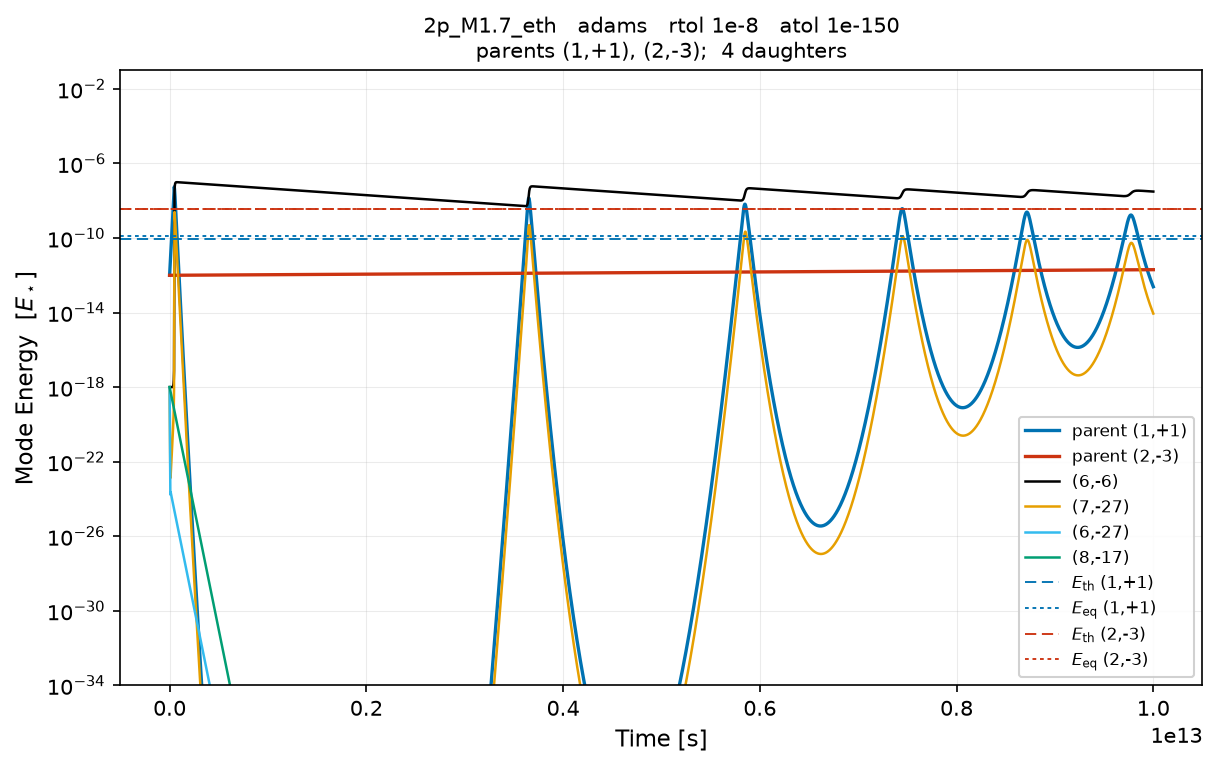
\includegraphics[width=0.21\textwidth,height=0.1323\textwidth]{../plots/adams/2p_M1.7_eth/r1e-8_a1e-150.png} & 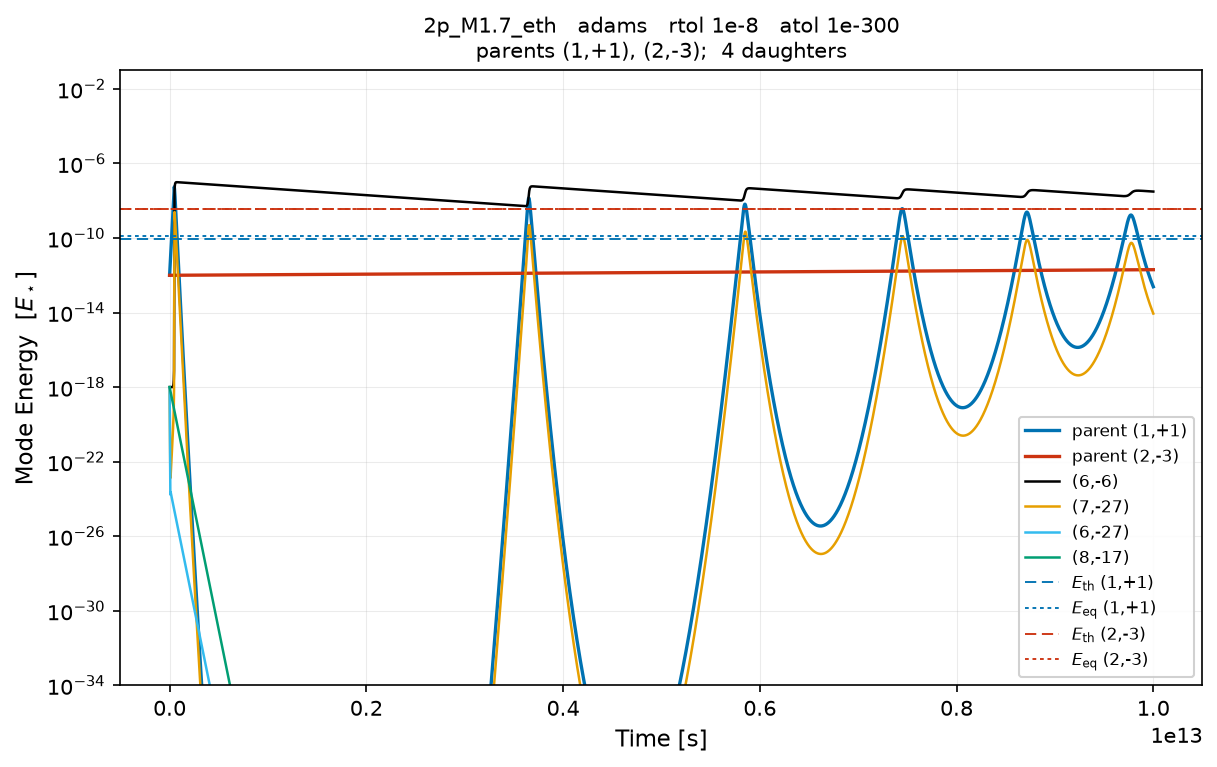
\includegraphics[width=0.21\textwidth,height=0.1323\textwidth]{../plots/adams/2p_M1.7_eth/r1e-8_a1e-300.png} & 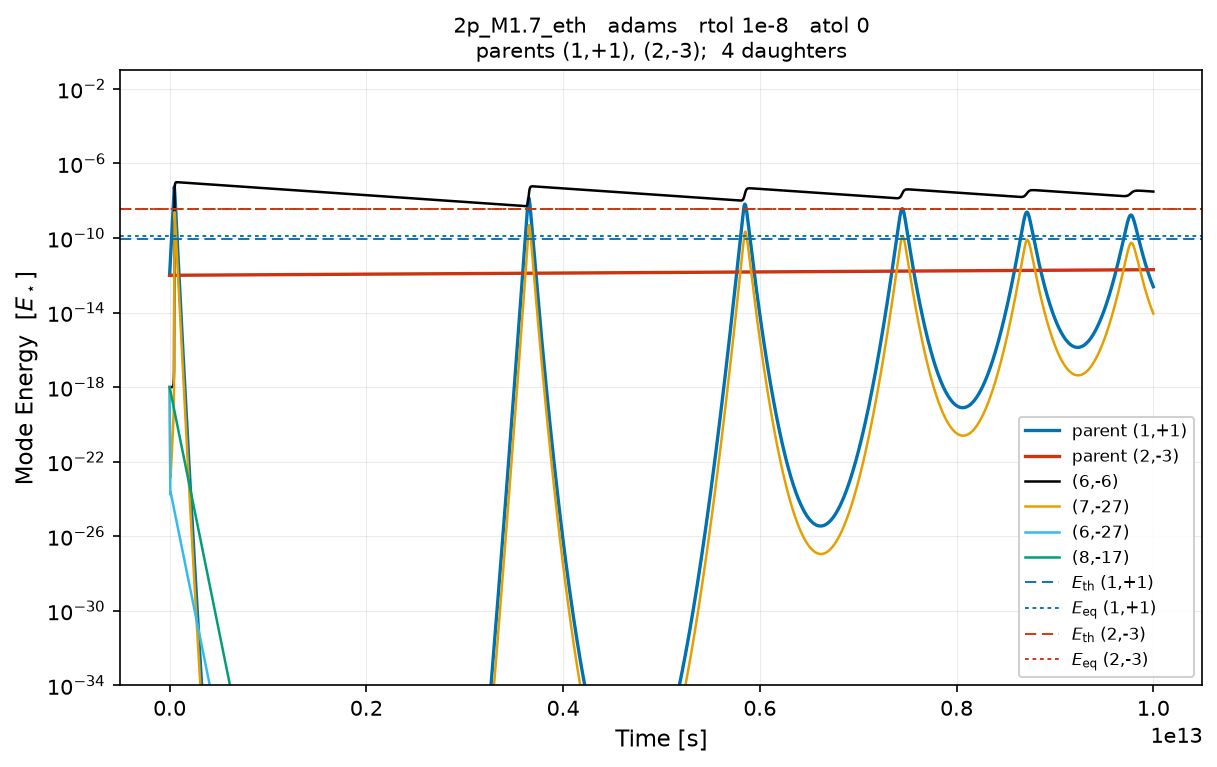
\includegraphics[width=0.21\textwidth,height=0.1323\textwidth]{../plots/adams/2p_M1.7_eth/r1e-8_a0.png} \\[-1pt]
 & \parbox[t]{0.21\textwidth}{\centering\scriptsize 5.42\,M steps, 9.2\,s} & \parbox[t]{0.21\textwidth}{\centering\scriptsize 5.69\,M steps, 9.5\,s} & \parbox[t]{0.21\textwidth}{\centering\scriptsize 5.69\,M steps, 5.6\,s} & \parbox[t]{0.21\textwidth}{\centering\scriptsize 5.69\,M steps, 6.3\,s} \\[2pt]
\end{tabular}\par}
\par\noindent{\scriptsize\setlength\tabcolsep{3.5pt}\renewcommand\arraystretch{0.92}
\begin{tabular}{@{}llllrrrrrrr@{}}
\toprule
integrator & atol & stop & $t_{\rm stop}$ [s] & steps & rejected & RHS & Jac. & NL it. & lin. it. & wall [s] \\
\midrule
rk8pd & $10^{-40}$ & end & $1.00\times10^{13}$ & 990.0\,k & 104.5\,k & 12.87\,M & -- & -- & -- & 1.9 \\
 & $10^{-150}$ & end & $1.00\times10^{13}$ & 1.13\,M & 128.5\,k & 14.69\,M & -- & -- & -- & 5.3 \\
 & $10^{-300}$ & end & $1.00\times10^{13}$ & 1.13\,M & 128.6\,k & 14.69\,M & -- & -- & -- & 3.3 \\
 & $0$ & end & $1.00\times10^{13}$ & 1.13\,M & 128.6\,k & 14.69\,M & -- & -- & -- & 5.3 \\
\addlinespace[2pt]
BDF, dense analytic Jacobian & $10^{-40}$ & end & $1.00\times10^{13}$ & 6.79\,M & 49.2\,k & 7.26\,M & 120.3\,k & 7.26\,M & -- & 8.6 \\
 & $10^{-150}$ & end & $1.00\times10^{13}$ & 13.11\,M & 133.6\,k & 14.11\,M & 230.1\,k & 14.11\,M & -- & 24.6 \\
 & $10^{-300}$ & end & $1.00\times10^{13}$ & 13.10\,M & 133.6\,k & 14.11\,M & 230.1\,k & 14.10\,M & -- & 18.9 \\
 & $0$ & end & $1.00\times10^{13}$ & 13.10\,M & 133.6\,k & 14.11\,M & 230.1\,k & 14.10\,M & -- & 21.0 \\
\addlinespace[2pt]
BDF-Krylov, band full & $10^{-40}$ & end & $1.00\times10^{13}$ & 1.98\,M & 16.0\,k & 4.65\,M & 37.6\,k & 2.12\,M & 2.08\,M & 3.2 \\
 & $10^{-150}$ & end & $1.00\times10^{13}$ & 12.77\,M & 148.3\,k & 29.89\,M & 223.9\,k & 13.86\,M & 13.34\,M & 33.2 \\
 & $10^{-300}$ & end & $1.00\times10^{13}$ & 12.78\,M & 147.9\,k & 29.90\,M & 224.0\,k & 13.86\,M & 13.34\,M & 19.5 \\
 & $0$ & end & $1.00\times10^{13}$ & 12.78\,M & 147.9\,k & 29.90\,M & 224.0\,k & 13.86\,M & 13.34\,M & 37.6 \\
\addlinespace[2pt]
BDF-Krylov, band 3 & $10^{-40}$ & end & $1.00\times10^{13}$ & 2.19\,M & 24.0\,k & 5.58\,M & 41.3\,k & 2.39\,M & 2.90\,M & 6.3 \\
 & $10^{-150}$ & end & $1.00\times10^{13}$ & 12.40\,M & 183.1\,k & 31.21\,M & 217.9\,k & 13.67\,M & 16.01\,M & 38.2 \\
 & $10^{-300}$ & end & $1.00\times10^{13}$ & 12.41\,M & 183.7\,k & 31.21\,M & 217.9\,k & 13.67\,M & 16.01\,M & 27.7 \\
 & $0$ & end & $1.00\times10^{13}$ & 12.41\,M & 183.7\,k & 31.21\,M & 217.9\,k & 13.67\,M & 16.01\,M & 24.7 \\
\addlinespace[2pt]
Adams, fixed point & $10^{-40}$ & end & $1.00\times10^{13}$ & 5.42\,M & 223.9\,k & 8.29\,M & -- & 8.29\,M & -- & 9.2 \\
 & $10^{-150}$ & end & $1.00\times10^{13}$ & 5.69\,M & 277.3\,k & 8.45\,M & -- & 8.44\,M & -- & 9.5 \\
 & $10^{-300}$ & end & $1.00\times10^{13}$ & 5.69\,M & 277.7\,k & 8.43\,M & -- & 8.43\,M & -- & 5.6 \\
 & $0$ & end & $1.00\times10^{13}$ & 5.69\,M & 277.7\,k & 8.43\,M & -- & 8.43\,M & -- & 6.3 \\
\bottomrule
\end{tabular}}

\clearpage
\subsection{\texttt{2p\_M2.0T\_eth}}\label{net:2p_M2.0T_eth}
\noindent\begin{minipage}[t]{0.43\textwidth}\vspace{0pt}\footnotesize
\begin{tabular}{@{}rrlrr@{}}
\toprule
id & gen & $(\ell,n)$ & $\omega$ [rad\,s$^{-1}$] & $\gamma$ [s$^{-1}$] \\
\midrule
0 & 0 & (2,$-$3) & $6.816\times10^{-4}$ & $-8.642\times10^{-13}$ \\
1 & 0 & (2,$-$2) & $7.959\times10^{-4}$ & $-6.697\times10^{-11}$ \\
2 & 1 & (14,$-$48) & $3.408\times10^{-4}$ & $1.376\times10^{-9}$ \\
3 & 1 & (3,$-$31) & $1.287\times10^{-4}$ & $8.096\times10^{-11}$ \\
4 & 1 & (5,$-$8) & $6.672\times10^{-4}$ & $7.367\times10^{-13}$ \\
\bottomrule
\end{tabular}
\end{minipage}\hfill
\begin{minipage}[t]{0.55\textwidth}\vspace{0pt}\footnotesize
\textbf{Model} \texttt{dsct\_M2.0\_T7696}, rule eth, $N=1$, cut 0.15,
closure 0.005; 5 modes, 2 triplet(s).\\[2pt]
\textbf{Selecting pairs}\\ (2,$-$3) $\to$ (14,$-$48) + (14,$-$48): $\Delta/\omega_a=-6.00\times10^{-6}$, $\kappa=-0.452$, $E_{\rm th}=6.40\times10^{-11}$, $E_{\rm eq}=6.40\times10^{-11}$\\
(2,$-$2) $\to$ (3,$-$31) + (5,$-$8): $\Delta/\omega_a=-3.69\times10^{-6}$, $\kappa=+0.215$, $E_{\rm th}=4.87\times10^{-12}$, $E_{\rm eq}=1.50\times10^{-10}$\\[2pt]
Daughter (14,$-48$) decays to $E\sim10^{-3600}$ in exact arithmetic; its regrowth time is set by each run's floor.
\end{minipage}

\par\smallskip{\centering\begin{tabular}{@{}c@{\hspace{2pt}}c@{\hspace{2pt}}c@{\hspace{2pt}}c@{\hspace{2pt}}c@{}}
 & \small atol $10^{-40}$ & \small atol $10^{-150}$ & \small atol $10^{-300}$ & \small atol $0$ \\[1pt]
\rotatebox{90}{\parbox{0.1323\textwidth}{\centering\scriptsize\bfseries rk8pd}} & 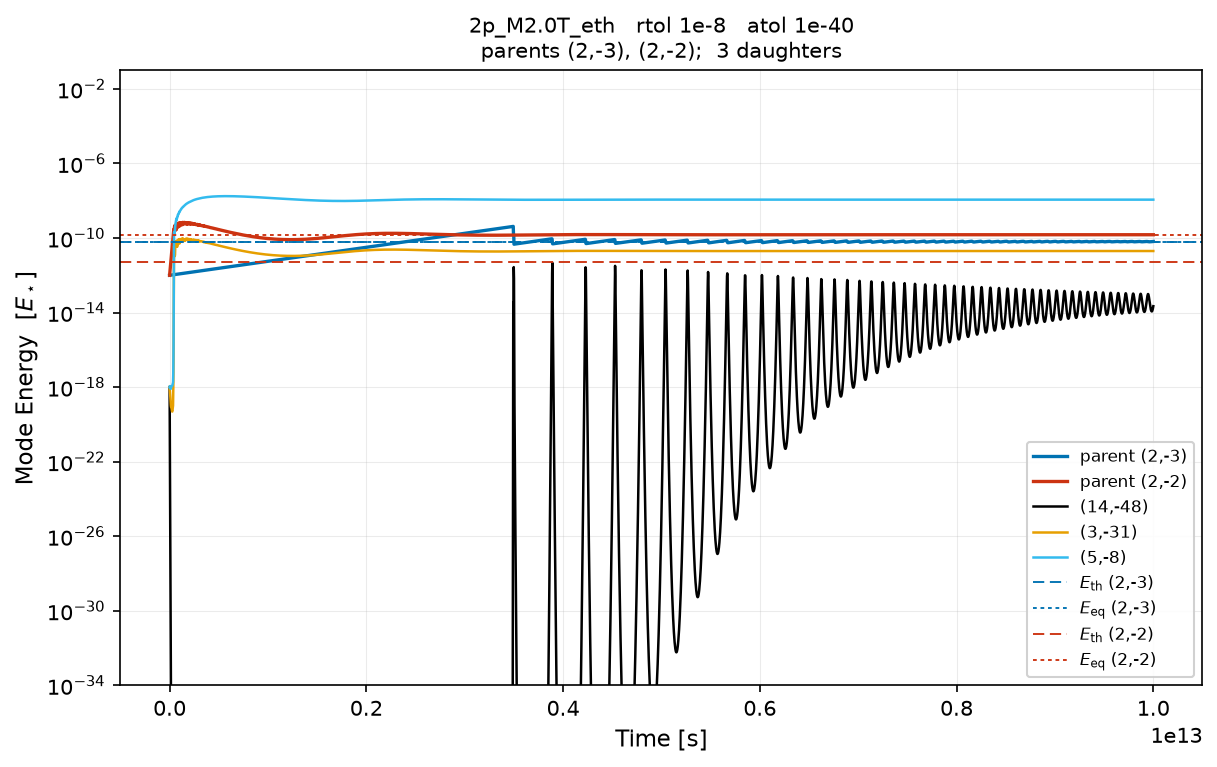
\includegraphics[width=0.21\textwidth,height=0.1323\textwidth]{../plots/rk8pd/2p_M2.0T_eth/r1e-8_a1e-40.png} & 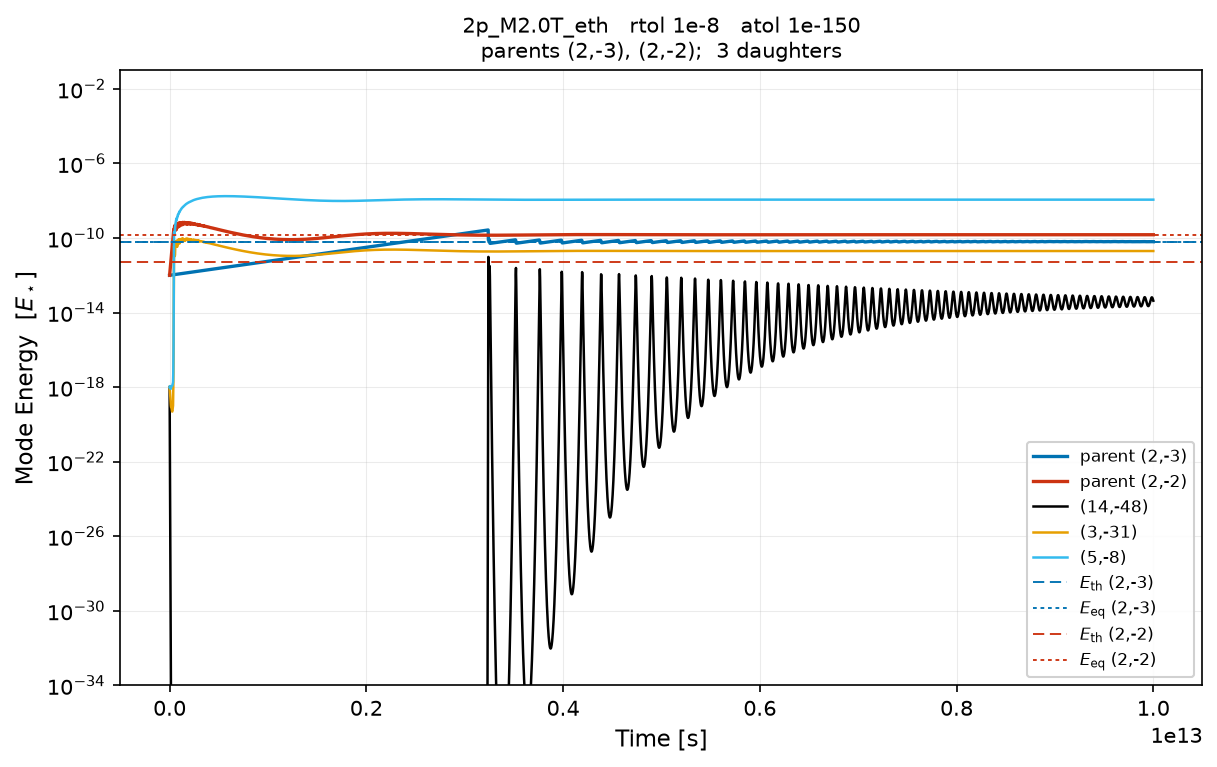
\includegraphics[width=0.21\textwidth,height=0.1323\textwidth]{../plots/rk8pd/2p_M2.0T_eth/r1e-8_a1e-150.png} & 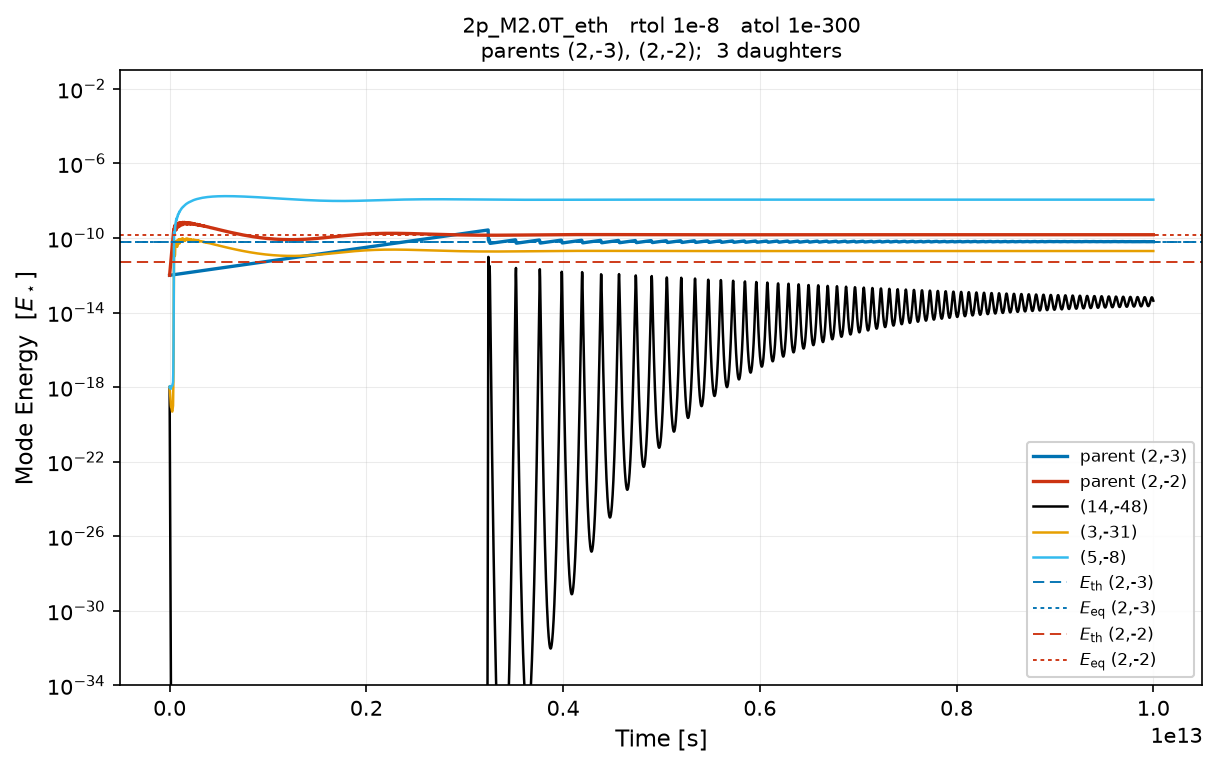
\includegraphics[width=0.21\textwidth,height=0.1323\textwidth]{../plots/rk8pd/2p_M2.0T_eth/r1e-8_a1e-300.png} & 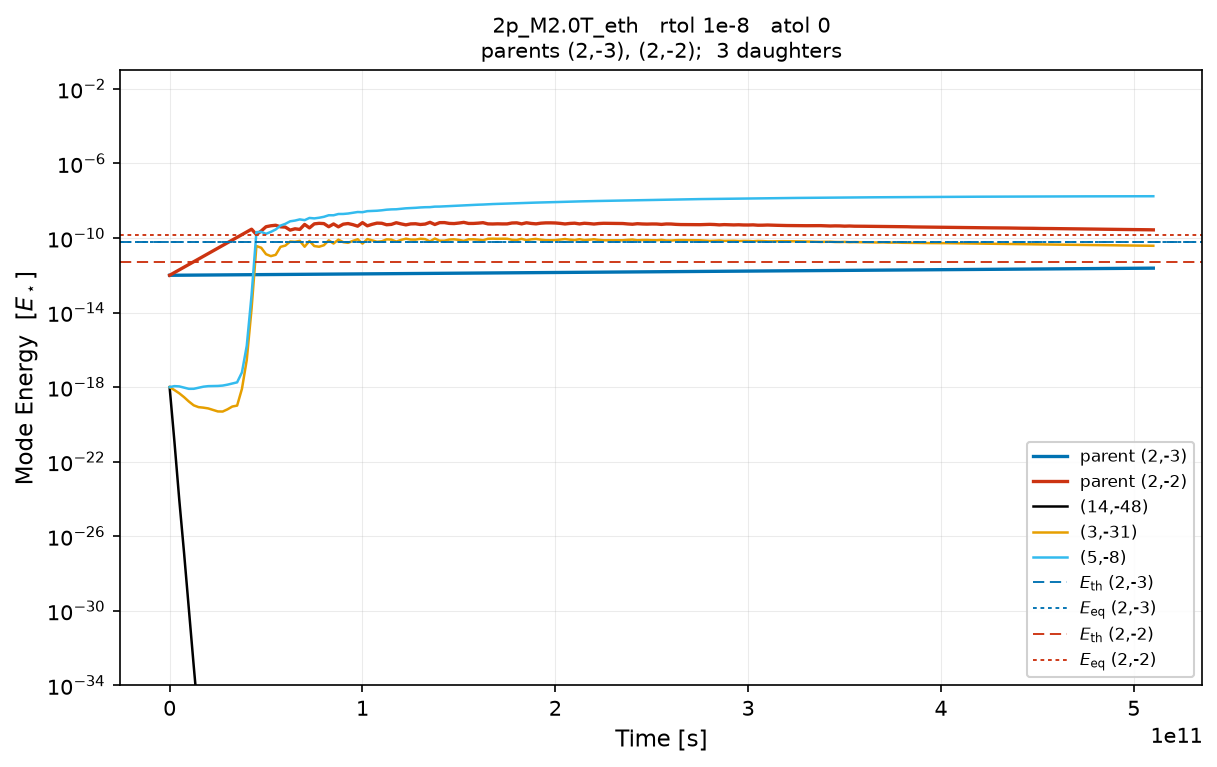
\includegraphics[width=0.21\textwidth,height=0.1323\textwidth]{../plots/rk8pd/2p_M2.0T_eth/r1e-8_a0.png} \\[-1pt]
 & \parbox[t]{0.21\textwidth}{\centering\scriptsize 385.6\,k steps, 1.5\,s} & \parbox[t]{0.21\textwidth}{\centering\scriptsize 385.4\,k steps, 9.3\,s} & \parbox[t]{0.21\textwidth}{\centering\scriptsize 385.4\,k steps, 2.4\,s} & \parbox[t]{0.21\textwidth}{\centering\scriptsize 50.17\,M steps, 1522.6\,s, wall} \\[2pt]
\rotatebox{90}{\parbox{0.1323\textwidth}{\centering\scriptsize\bfseries BDF, dense analytic Jacobian}} & 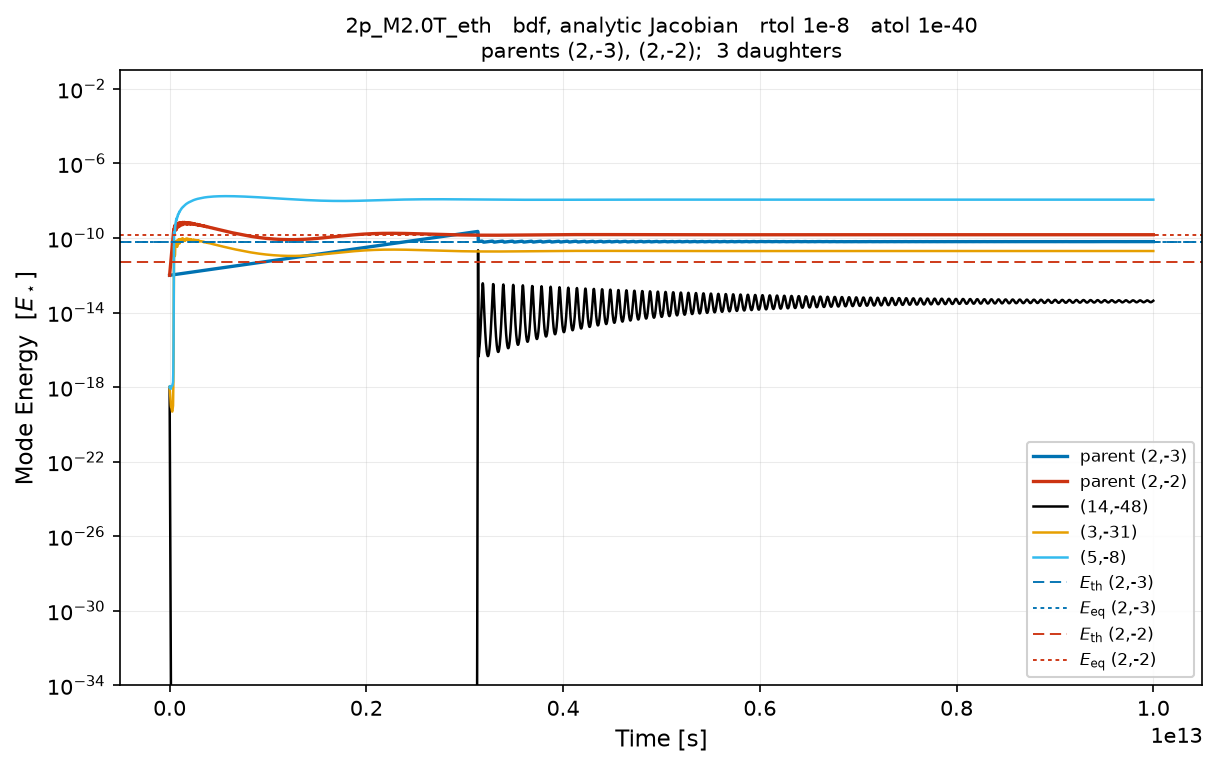
\includegraphics[width=0.21\textwidth,height=0.1323\textwidth]{../plots/bdf/2p_M2.0T_eth/r1e-8_a1e-40.png} & 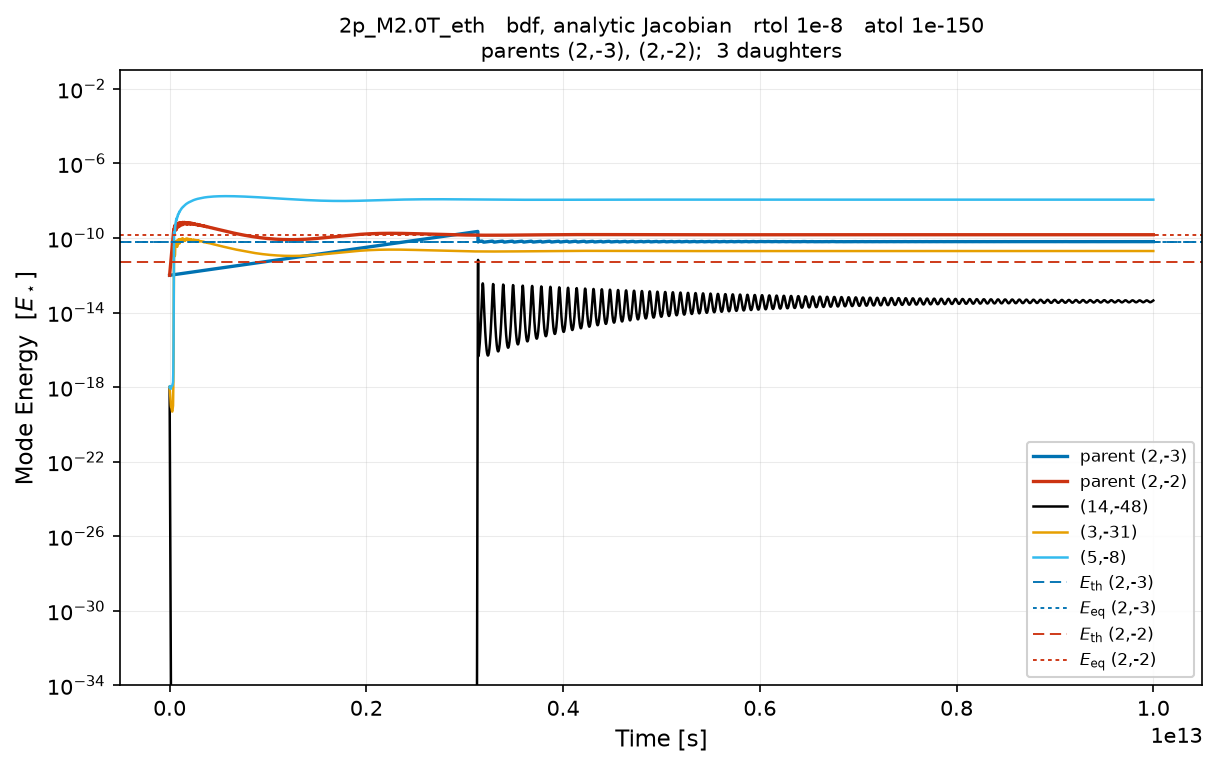
\includegraphics[width=0.21\textwidth,height=0.1323\textwidth]{../plots/bdf/2p_M2.0T_eth/r1e-8_a1e-150.png} & 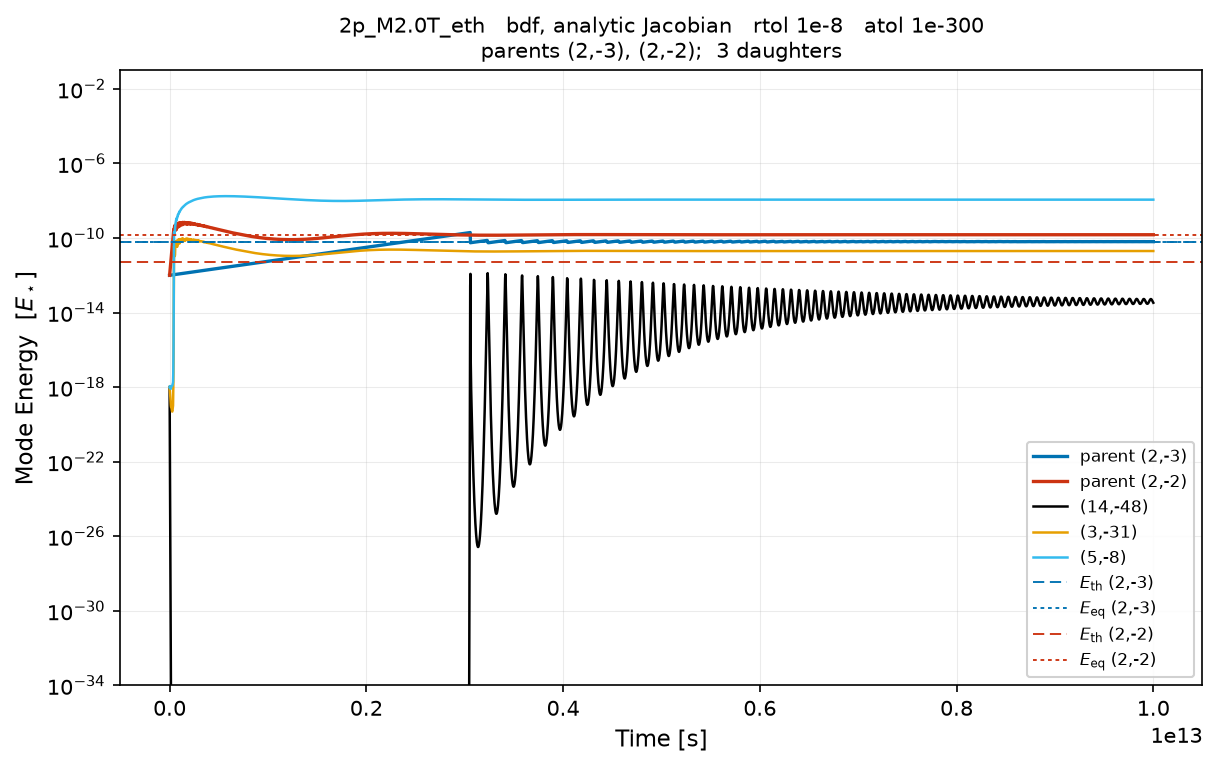
\includegraphics[width=0.21\textwidth,height=0.1323\textwidth]{../plots/bdf/2p_M2.0T_eth/r1e-8_a1e-300.png} & 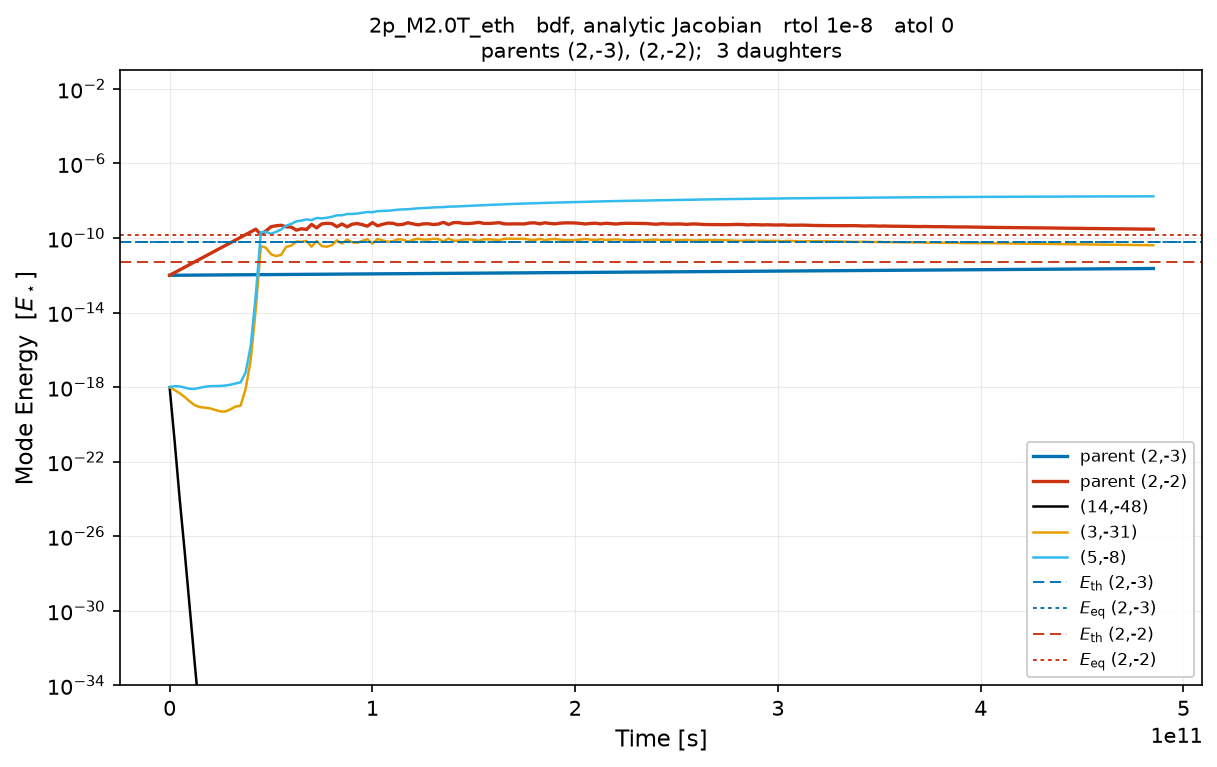
\includegraphics[width=0.21\textwidth,height=0.1323\textwidth]{../plots/bdf/2p_M2.0T_eth/r1e-8_a0.png} \\[-1pt]
 & \parbox[t]{0.21\textwidth}{\centering\scriptsize 3.45\,M steps, 3.7\,s} & \parbox[t]{0.21\textwidth}{\centering\scriptsize 3.45\,M steps, 13.0\,s} & \parbox[t]{0.21\textwidth}{\centering\scriptsize 3.45\,M steps, 4.3\,s} & \parbox[t]{0.21\textwidth}{\centering\scriptsize 145.3\,k steps, 0.4\,s, failed} \\[2pt]
\rotatebox{90}{\parbox{0.1323\textwidth}{\centering\scriptsize\bfseries BDF-Krylov, band full}} & 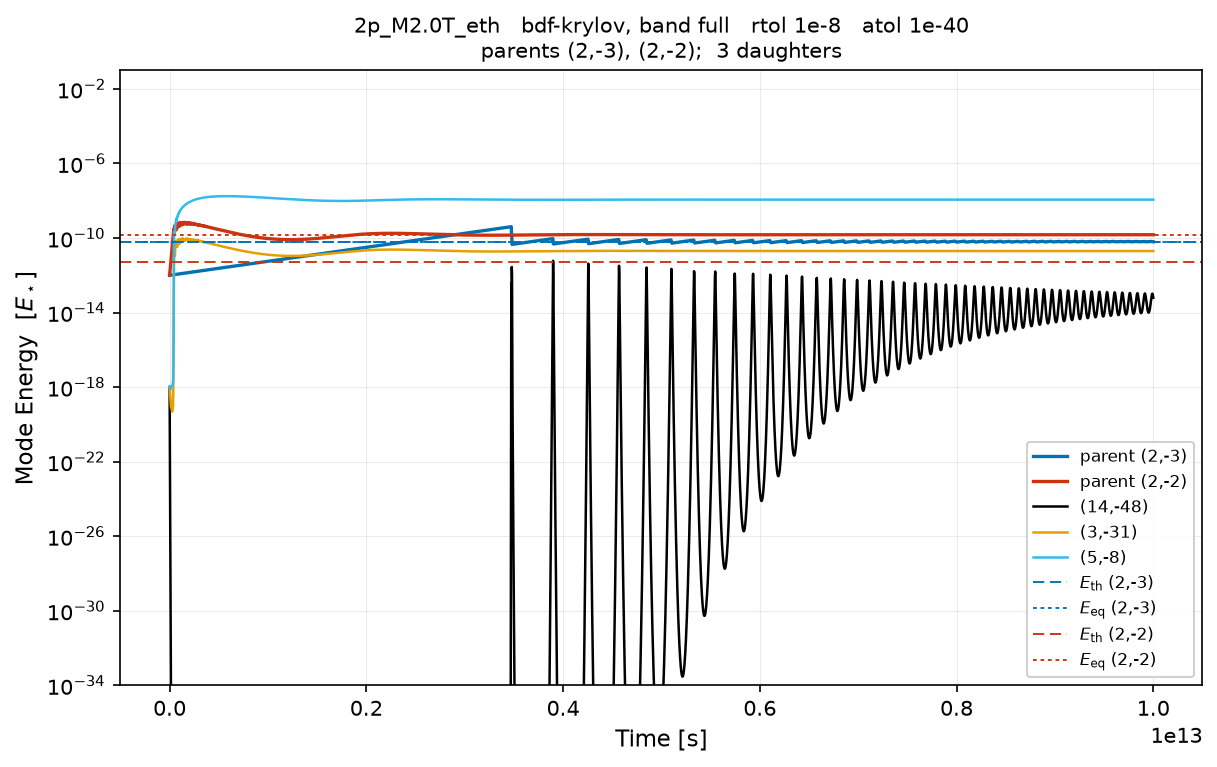
\includegraphics[width=0.21\textwidth,height=0.1323\textwidth]{../plots/krylov_full/2p_M2.0T_eth/r1e-8_a1e-40.png} & 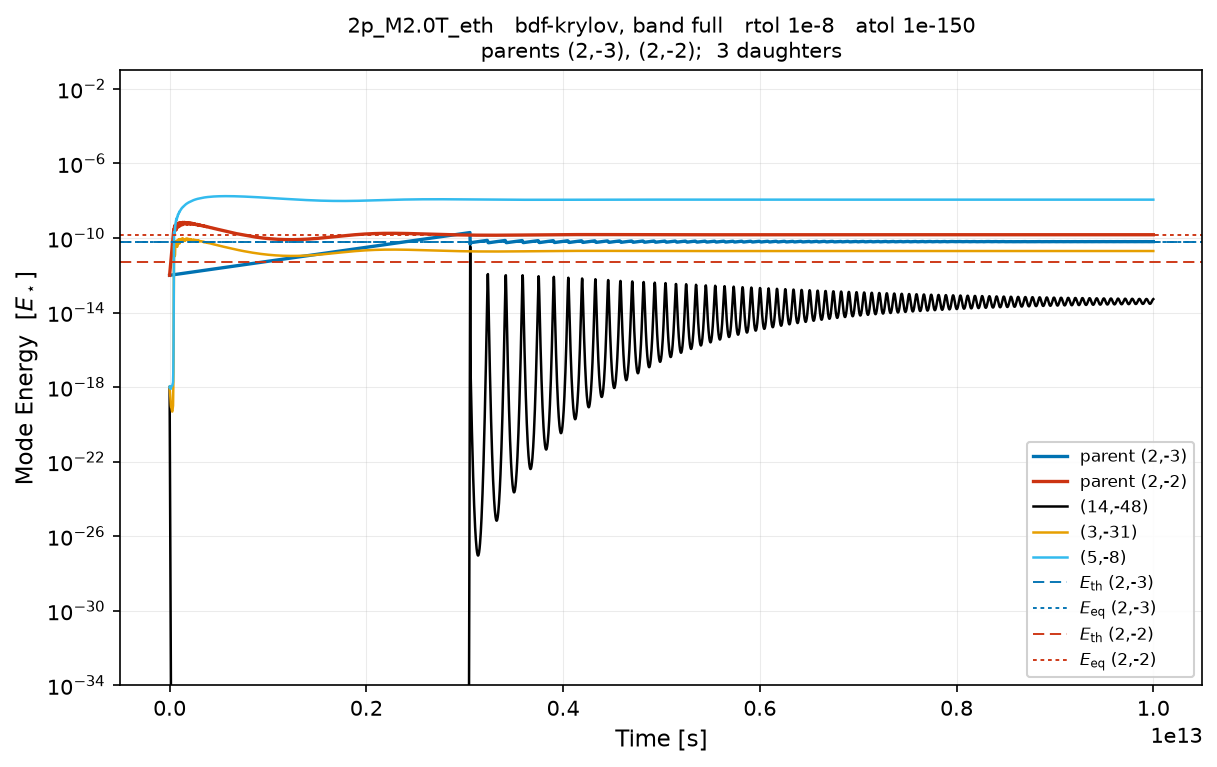
\includegraphics[width=0.21\textwidth,height=0.1323\textwidth]{../plots/krylov_full/2p_M2.0T_eth/r1e-8_a1e-150.png} & 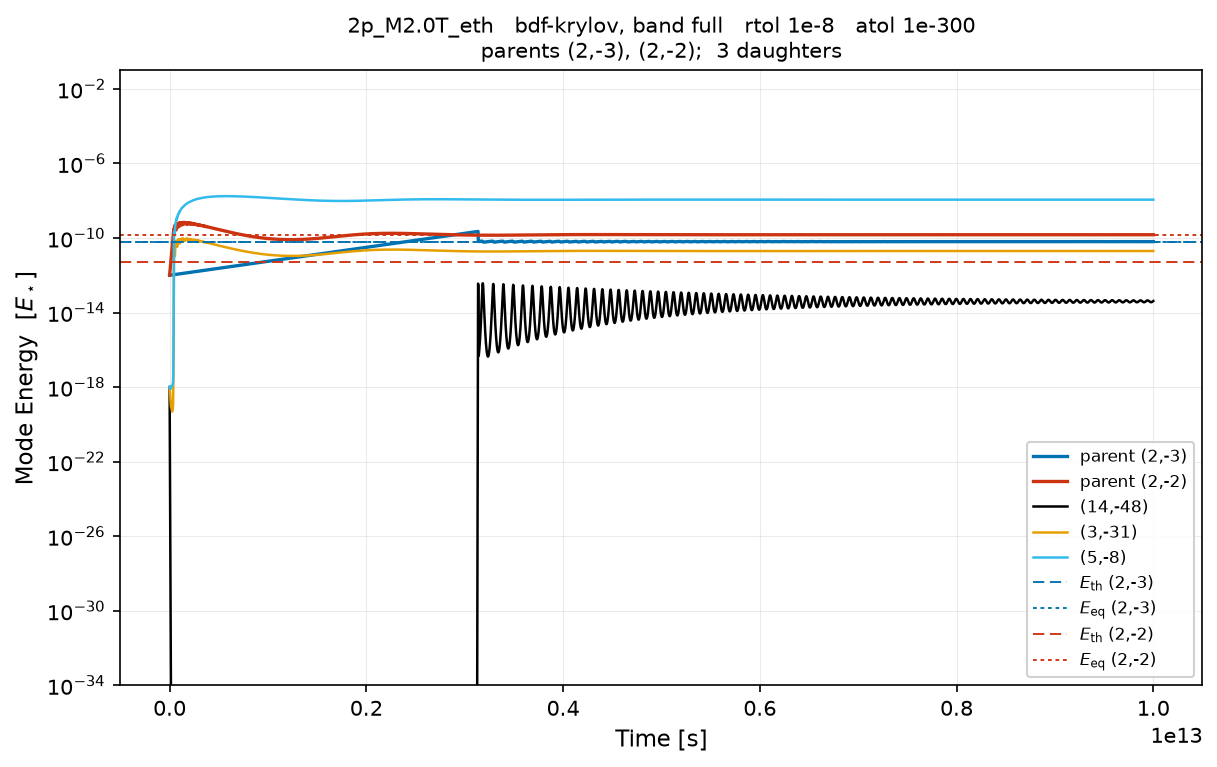
\includegraphics[width=0.21\textwidth,height=0.1323\textwidth]{../plots/krylov_full/2p_M2.0T_eth/r1e-8_a1e-300.png} & 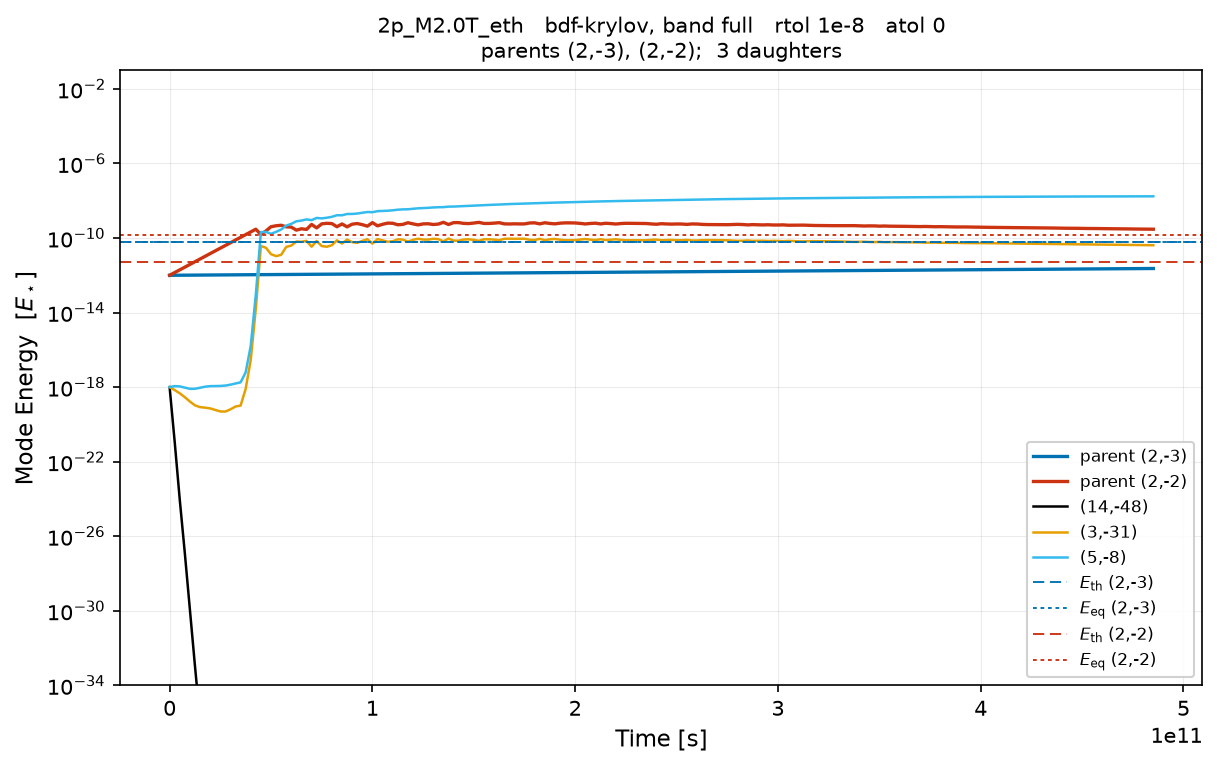
\includegraphics[width=0.21\textwidth,height=0.1323\textwidth]{../plots/krylov_full/2p_M2.0T_eth/r1e-8_a0.png} \\[-1pt]
 & \parbox[t]{0.21\textwidth}{\centering\scriptsize 3.41\,M steps, 10.0\,s} & \parbox[t]{0.21\textwidth}{\centering\scriptsize 3.40\,M steps, 7.4\,s} & \parbox[t]{0.21\textwidth}{\centering\scriptsize 3.41\,M steps, 18.4\,s} & \parbox[t]{0.21\textwidth}{\centering\scriptsize 143.2\,k steps, 0.6\,s, failed} \\[2pt]
\rotatebox{90}{\parbox{0.1323\textwidth}{\centering\scriptsize\bfseries BDF-Krylov, band 3}} & 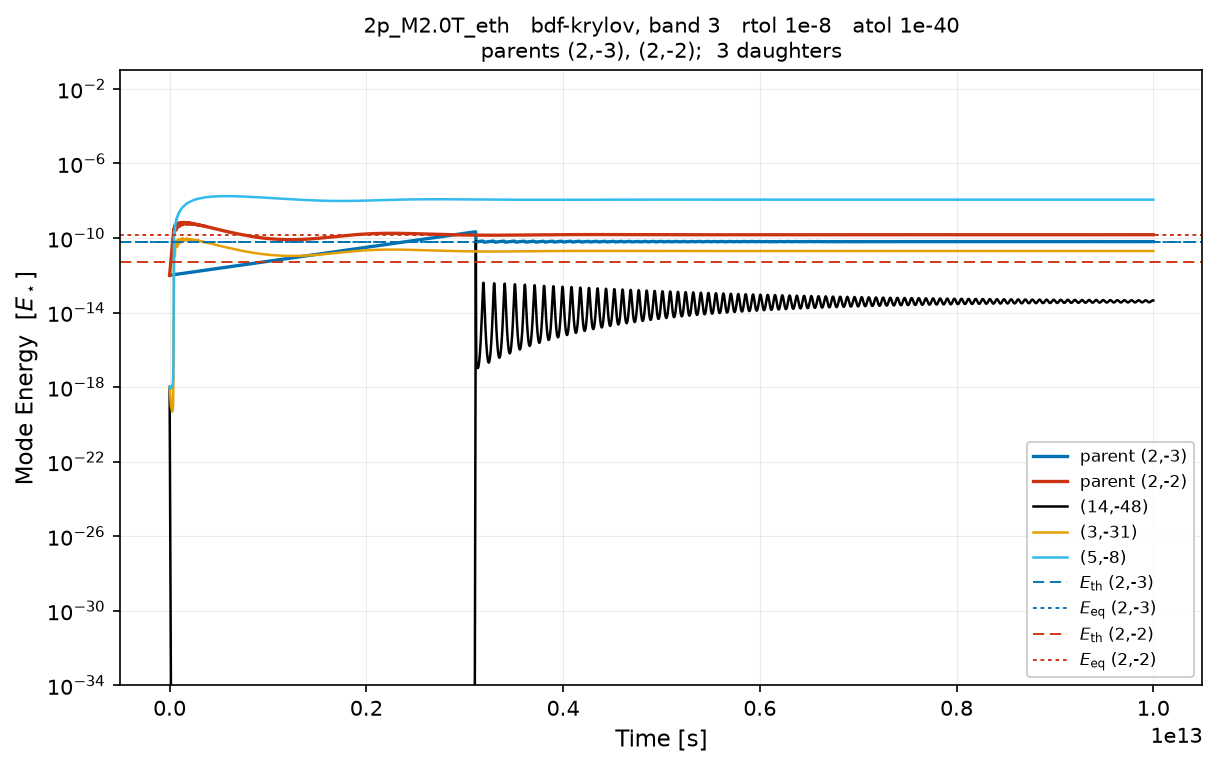
\includegraphics[width=0.21\textwidth,height=0.1323\textwidth]{../plots/krylov_b3/2p_M2.0T_eth/r1e-8_a1e-40.png} & 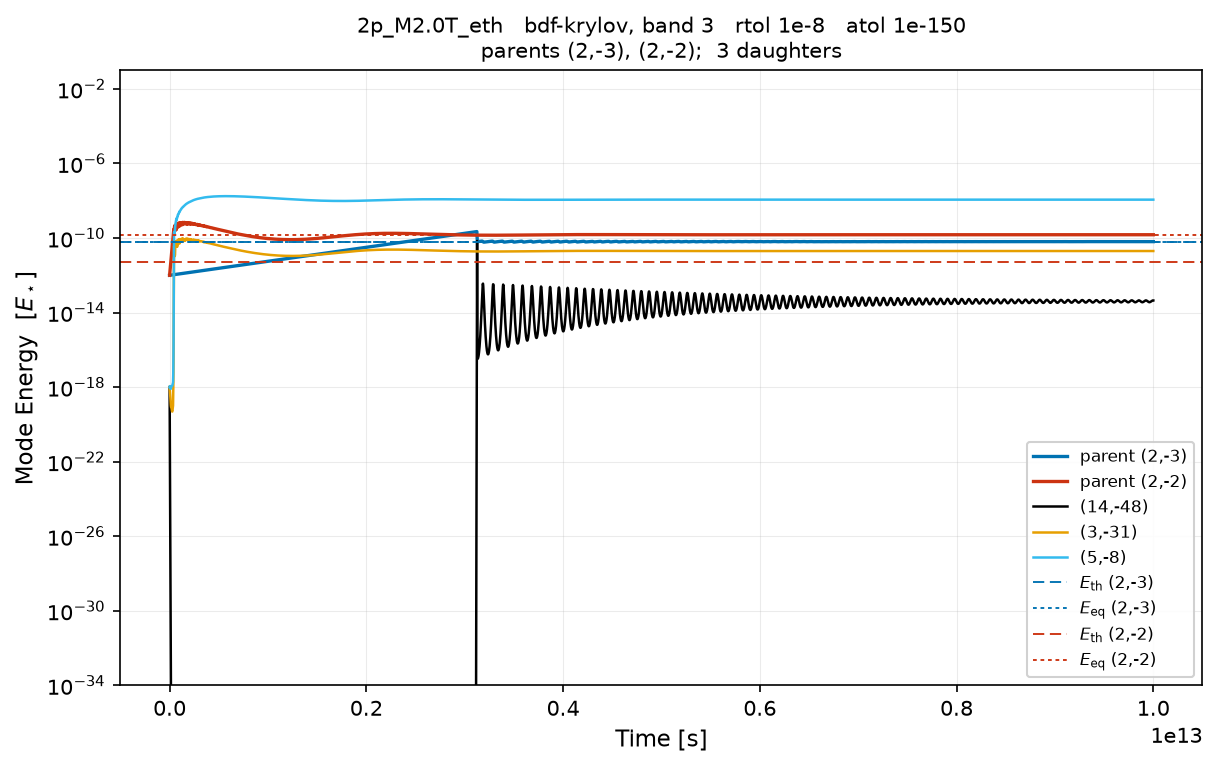
\includegraphics[width=0.21\textwidth,height=0.1323\textwidth]{../plots/krylov_b3/2p_M2.0T_eth/r1e-8_a1e-150.png} & 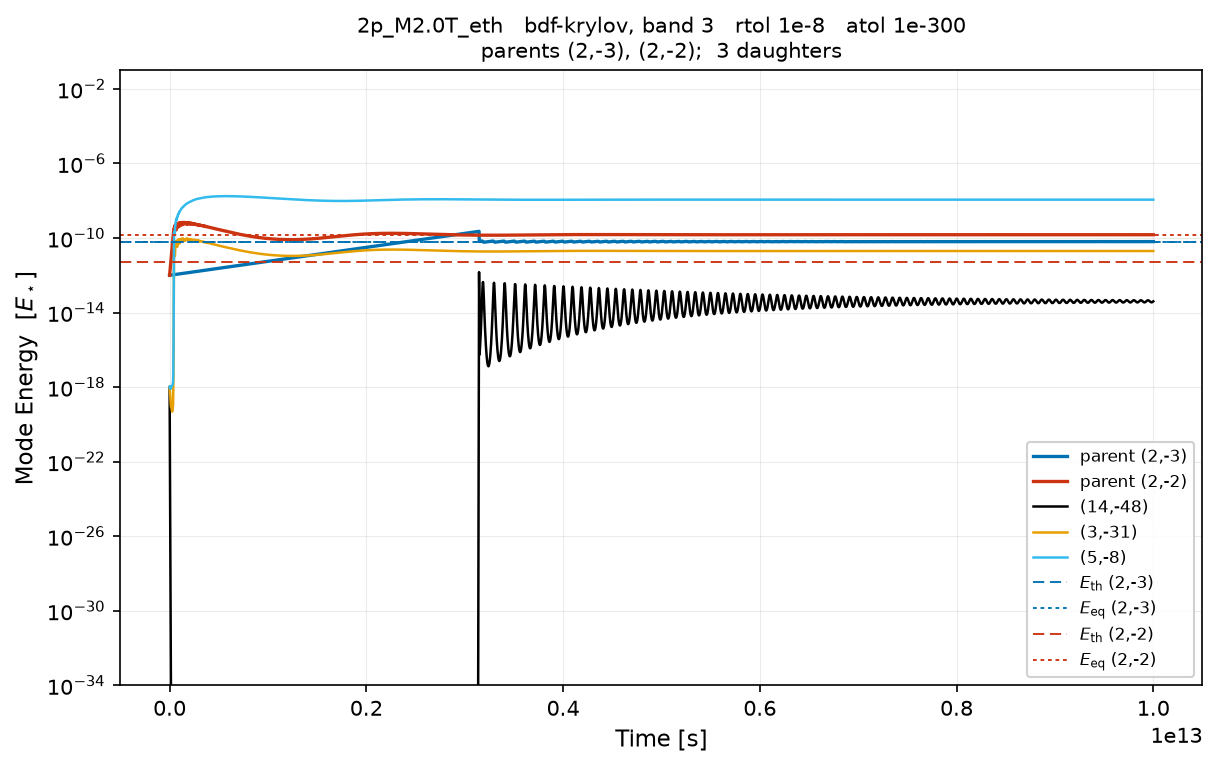
\includegraphics[width=0.21\textwidth,height=0.1323\textwidth]{../plots/krylov_b3/2p_M2.0T_eth/r1e-8_a1e-300.png} & 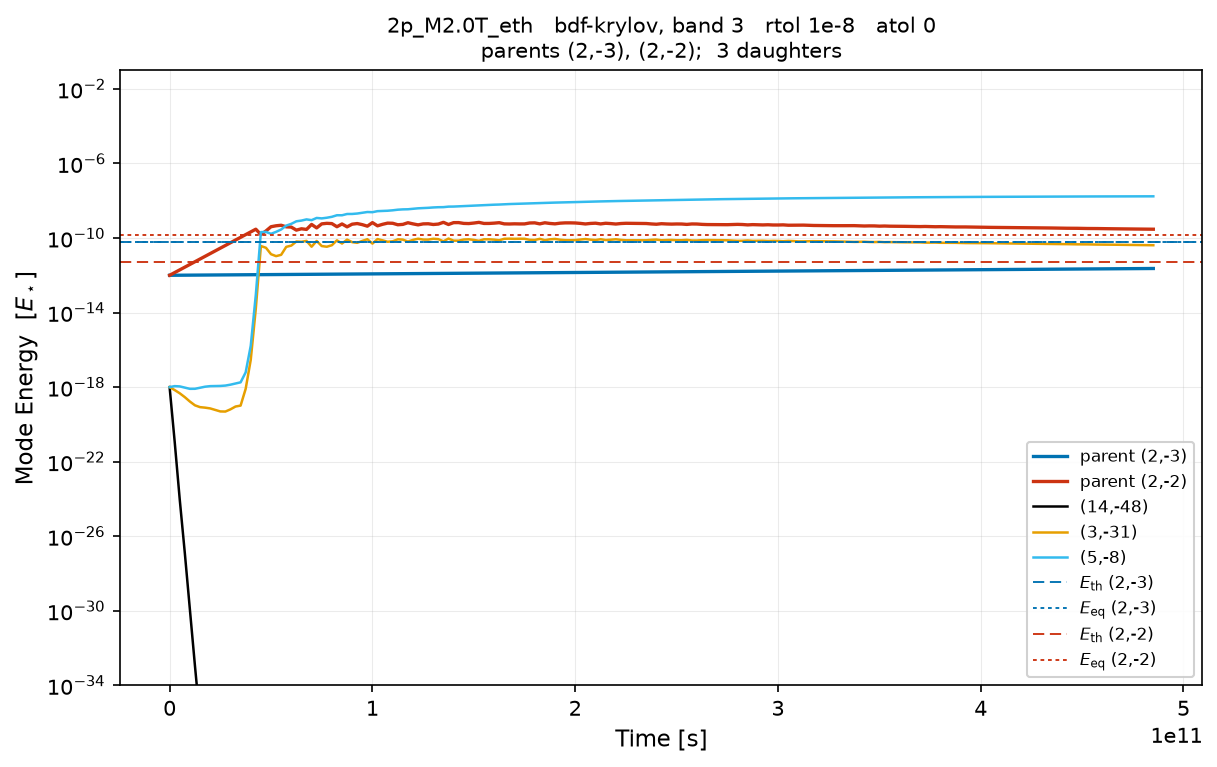
\includegraphics[width=0.21\textwidth,height=0.1323\textwidth]{../plots/krylov_b3/2p_M2.0T_eth/r1e-8_a0.png} \\[-1pt]
 & \parbox[t]{0.21\textwidth}{\centering\scriptsize 3.32\,M steps, 18.6\,s} & \parbox[t]{0.21\textwidth}{\centering\scriptsize 3.32\,M steps, 20.7\,s} & \parbox[t]{0.21\textwidth}{\centering\scriptsize 3.32\,M steps, 17.6\,s} & \parbox[t]{0.21\textwidth}{\centering\scriptsize 141.8\,k steps, 0.2\,s, failed} \\[2pt]
\rotatebox{90}{\parbox{0.1323\textwidth}{\centering\scriptsize\bfseries Adams, fixed point}} & 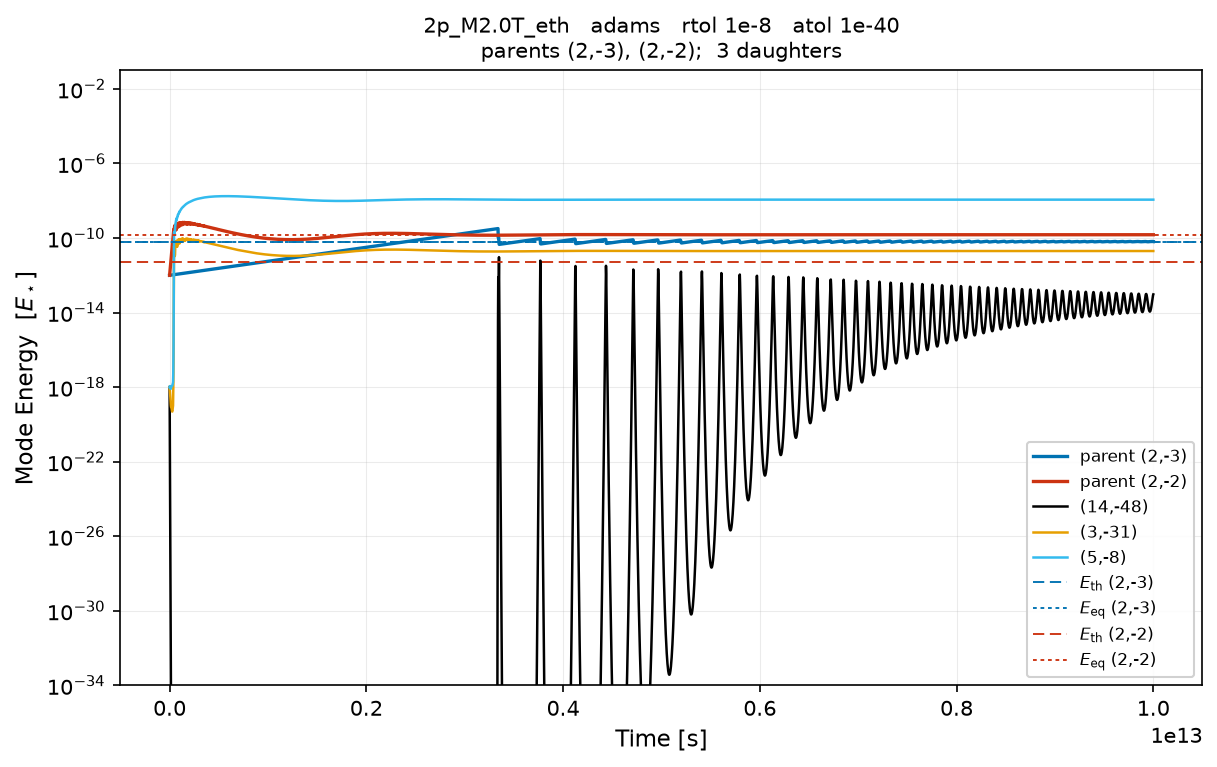
\includegraphics[width=0.21\textwidth,height=0.1323\textwidth]{../plots/adams/2p_M2.0T_eth/r1e-8_a1e-40.png} & 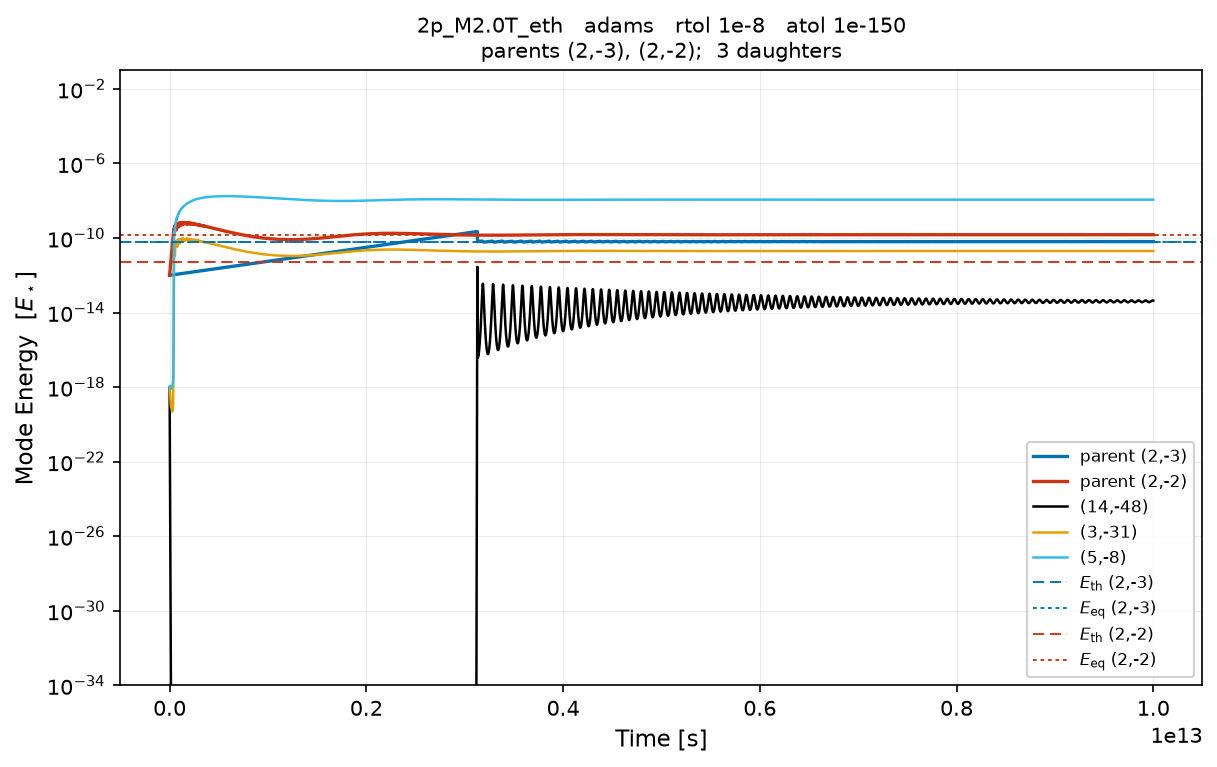
\includegraphics[width=0.21\textwidth,height=0.1323\textwidth]{../plots/adams/2p_M2.0T_eth/r1e-8_a1e-150.png} & 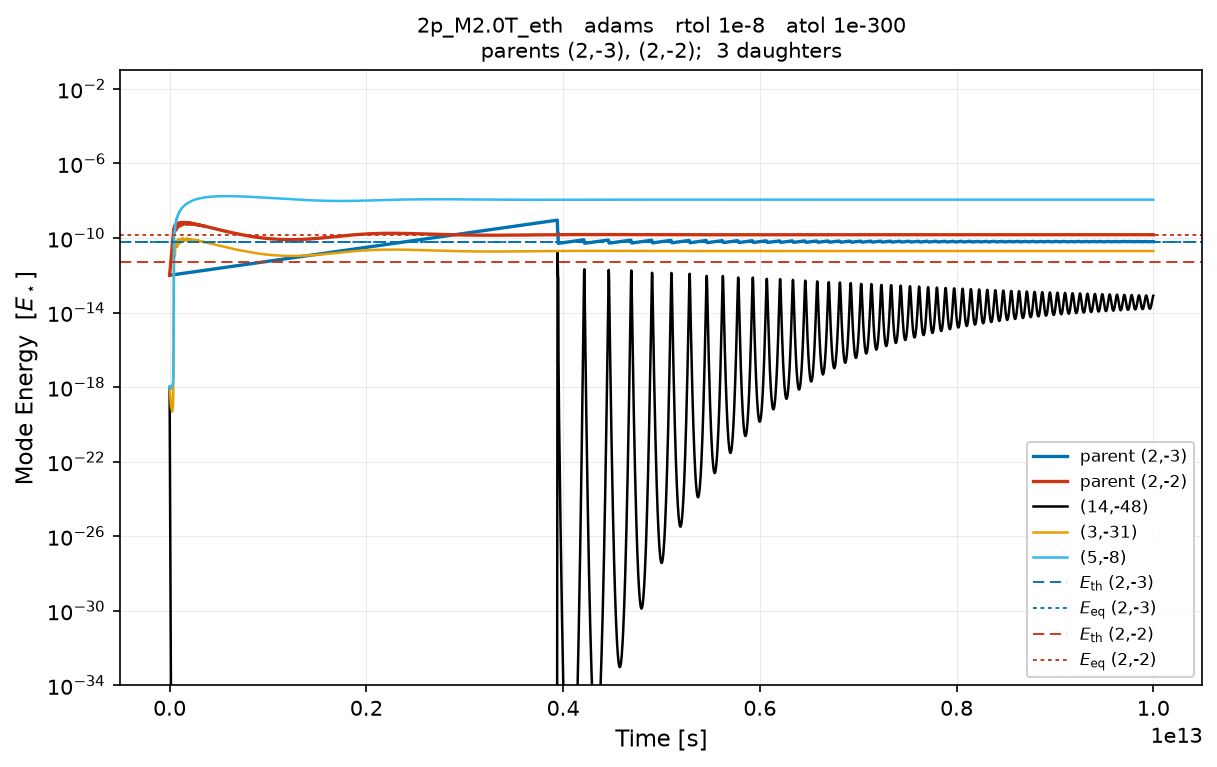
\includegraphics[width=0.21\textwidth,height=0.1323\textwidth]{../plots/adams/2p_M2.0T_eth/r1e-8_a1e-300.png} & 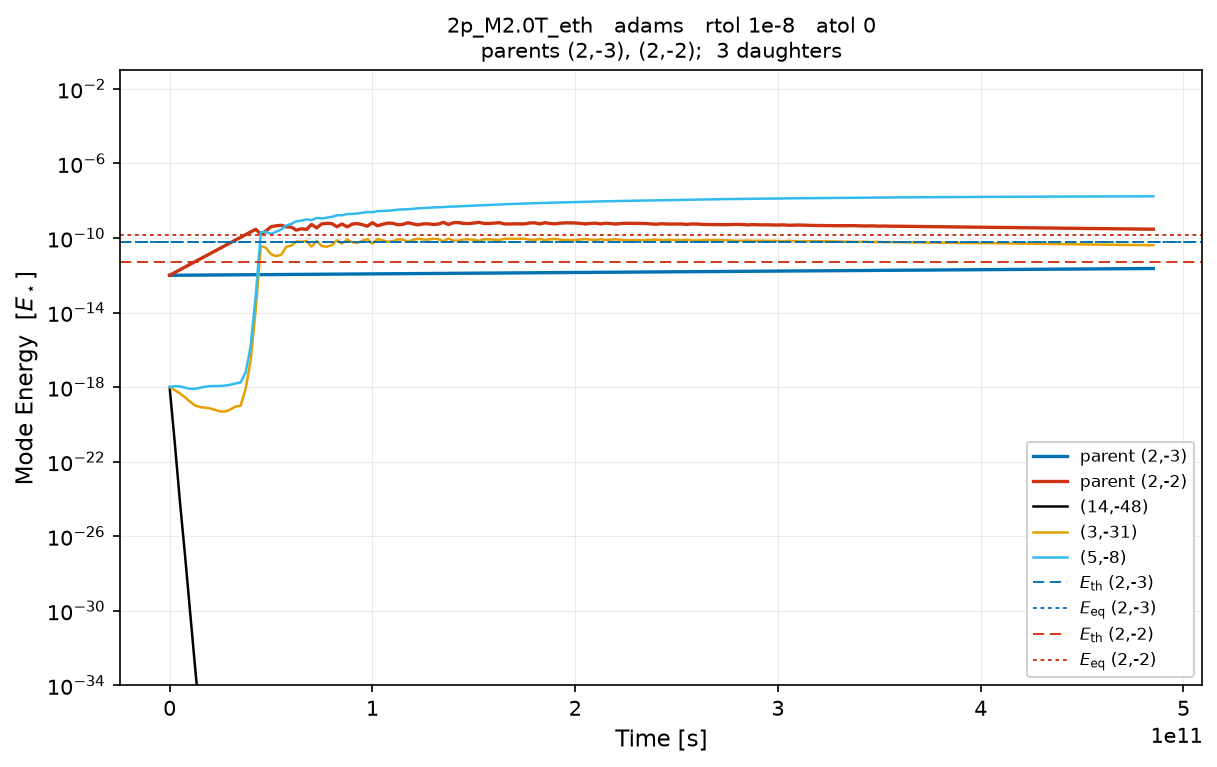
\includegraphics[width=0.21\textwidth,height=0.1323\textwidth]{../plots/adams/2p_M2.0T_eth/r1e-8_a0.png} \\[-1pt]
 & \parbox[t]{0.21\textwidth}{\centering\scriptsize 2.00\,M steps, 6.4\,s} & \parbox[t]{0.21\textwidth}{\centering\scriptsize 2.00\,M steps, 2.1\,s} & \parbox[t]{0.21\textwidth}{\centering\scriptsize 2.00\,M steps, 7.0\,s} & \parbox[t]{0.21\textwidth}{\centering\scriptsize 84.3\,k steps, 0.2\,s, failed} \\[2pt]
\end{tabular}\par}
\par\noindent{\scriptsize\setlength\tabcolsep{3.5pt}\renewcommand\arraystretch{0.92}
\begin{tabular}{@{}llllrrrrrrr@{}}
\toprule
integrator & atol & stop & $t_{\rm stop}$ [s] & steps & rejected & RHS & Jac. & NL it. & lin. it. & wall [s] \\
\midrule
rk8pd & $10^{-40}$ & end & $1.00\times10^{13}$ & 385.6\,k & 83.9\,k & 5.01\,M & -- & -- & -- & 1.5 \\
 & $10^{-150}$ & end & $1.00\times10^{13}$ & 385.4\,k & 83.7\,k & 5.01\,M & -- & -- & -- & 9.3 \\
 & $10^{-300}$ & end & $1.00\times10^{13}$ & 385.4\,k & 83.7\,k & 5.01\,M & -- & -- & -- & 2.4 \\
 & $0$ & wall & $5.10\times10^{11}$ & 50.17\,M & 56.1\,k & 652.18\,M & -- & -- & -- & 1522.6 \\
\addlinespace[2pt]
BDF, dense analytic Jacobian & $10^{-40}$ & end & $1.00\times10^{13}$ & 3.45\,M & 57.6\,k & 3.84\,M & 72.5\,k & 3.83\,M & -- & 3.7 \\
 & $10^{-150}$ & end & $1.00\times10^{13}$ & 3.45\,M & 57.4\,k & 3.84\,M & 72.5\,k & 3.83\,M & -- & 13.0 \\
 & $10^{-300}$ & end & $1.00\times10^{13}$ & 3.45\,M & 57.3\,k & 3.84\,M & 72.5\,k & 3.83\,M & -- & 4.3 \\
 & $0$ & failed & $4.85\times10^{11}$ & 145.3\,k & 3.9\,k & 167.3\,k & 3.2\,k & 167.1\,k & -- & 0.4 \\
\addlinespace[2pt]
BDF-Krylov, band full & $10^{-40}$ & end & $1.00\times10^{13}$ & 3.41\,M & 60.6\,k & 7.96\,M & 71.0\,k & 3.77\,M & 3.48\,M & 10.0 \\
 & $10^{-150}$ & end & $1.00\times10^{13}$ & 3.40\,M & 61.2\,k & 7.95\,M & 71.0\,k & 3.76\,M & 3.48\,M & 7.4 \\
 & $10^{-300}$ & end & $1.00\times10^{13}$ & 3.41\,M & 60.7\,k & 7.96\,M & 71.0\,k & 3.77\,M & 3.48\,M & 18.4 \\
 & $0$ & failed & $4.85\times10^{11}$ & 143.2\,k & 3.7\,k & 342.1\,k & 3.1\,k & 162.9\,k & 148.4\,k & 0.6 \\
\addlinespace[2pt]
BDF-Krylov, band 3 & $10^{-40}$ & end & $1.00\times10^{13}$ & 3.32\,M & 67.5\,k & 8.56\,M & 69.7\,k & 3.72\,M & 4.35\,M & 18.6 \\
 & $10^{-150}$ & end & $1.00\times10^{13}$ & 3.32\,M & 68.1\,k & 8.57\,M & 69.6\,k & 3.71\,M & 4.36\,M & 20.7 \\
 & $10^{-300}$ & end & $1.00\times10^{13}$ & 3.32\,M & 68.0\,k & 8.57\,M & 69.7\,k & 3.72\,M & 4.37\,M & 17.6 \\
 & $0$ & failed & $4.85\times10^{11}$ & 141.8\,k & 4.0\,k & 367.9\,k & 3.0\,k & 162.9\,k & 183.5\,k & 0.2 \\
\addlinespace[2pt]
Adams, fixed point & $10^{-40}$ & end & $1.00\times10^{13}$ & 2.00\,M & 131.7\,k & 3.30\,M & -- & 3.30\,M & -- & 6.4 \\
 & $10^{-150}$ & end & $1.00\times10^{13}$ & 2.00\,M & 132.1\,k & 3.30\,M & -- & 3.29\,M & -- & 2.1 \\
 & $10^{-300}$ & end & $1.00\times10^{13}$ & 2.00\,M & 132.3\,k & 3.30\,M & -- & 3.29\,M & -- & 7.0 \\
 & $0$ & failed & $4.85\times10^{11}$ & 84.3\,k & 5.9\,k & 138.5\,k & -- & 138.3\,k & -- & 0.2 \\
\bottomrule
\end{tabular}}

\clearpage
\subsection{\texttt{2p\_M2.0\_eeq}}\label{net:2p_M2.0_eeq}
\noindent\begin{minipage}[t]{0.43\textwidth}\vspace{0pt}\footnotesize
\begin{tabular}{@{}rrlrr@{}}
\toprule
id & gen & $(\ell,n)$ & $\omega$ [rad\,s$^{-1}$] & $\gamma$ [s$^{-1}$] \\
\midrule
0 & 0 & (1,$-$1) & $7.581\times10^{-4}$ & $-2.276\times10^{-10}$ \\
1 & 0 & (2,$-$2) & $7.710\times10^{-4}$ & $-1.619\times10^{-10}$ \\
2 & 1 & (5,$-$9) & $6.198\times10^{-4}$ & $4.584\times10^{-13}$ \\
3 & 1 & (6,$-$56) & $1.377\times10^{-4}$ & $2.817\times10^{-9}$ \\
4 & 1 & (6,$-$11) & $5.949\times10^{-4}$ & $1.643\times10^{-12}$ \\
5 & 1 & (8,$-$57) & $1.762\times10^{-4}$ & $4.129\times10^{-9}$ \\
\bottomrule
\end{tabular}
\end{minipage}\hfill
\begin{minipage}[t]{0.55\textwidth}\vspace{0pt}\footnotesize
\textbf{Model} \texttt{dsct\_M2.0}, rule eeq, $N=1$, cut 0.15,
closure 0.005; 6 modes, 2 triplet(s).\\[2pt]
\textbf{Selecting pairs}\\ (1,$-$1) $\to$ (5,$-$9) + (6,$-$56): $\Delta/\omega_a=-6.83\times10^{-4}$, $\kappa=+0.085$, $E_{\rm th}=1.75\times10^{-8}$, $E_{\rm eq}=2.07\times10^{-8}$\\
(2,$-$2) $\to$ (6,$-$11) + (8,$-$57): $\Delta/\omega_a=1.36\times10^{-4}$, $\kappa=+0.023$, $E_{\rm th}=1.97\times10^{-8}$, $E_{\rm eq}=2.13\times10^{-8}$\\[2pt]
Deep dips between bursts.
\end{minipage}

\par\smallskip{\centering\begin{tabular}{@{}c@{\hspace{2pt}}c@{\hspace{2pt}}c@{\hspace{2pt}}c@{\hspace{2pt}}c@{}}
 & \small atol $10^{-40}$ & \small atol $10^{-150}$ & \small atol $10^{-300}$ & \small atol $0$ \\[1pt]
\rotatebox{90}{\parbox{0.1323\textwidth}{\centering\scriptsize\bfseries rk8pd}} & 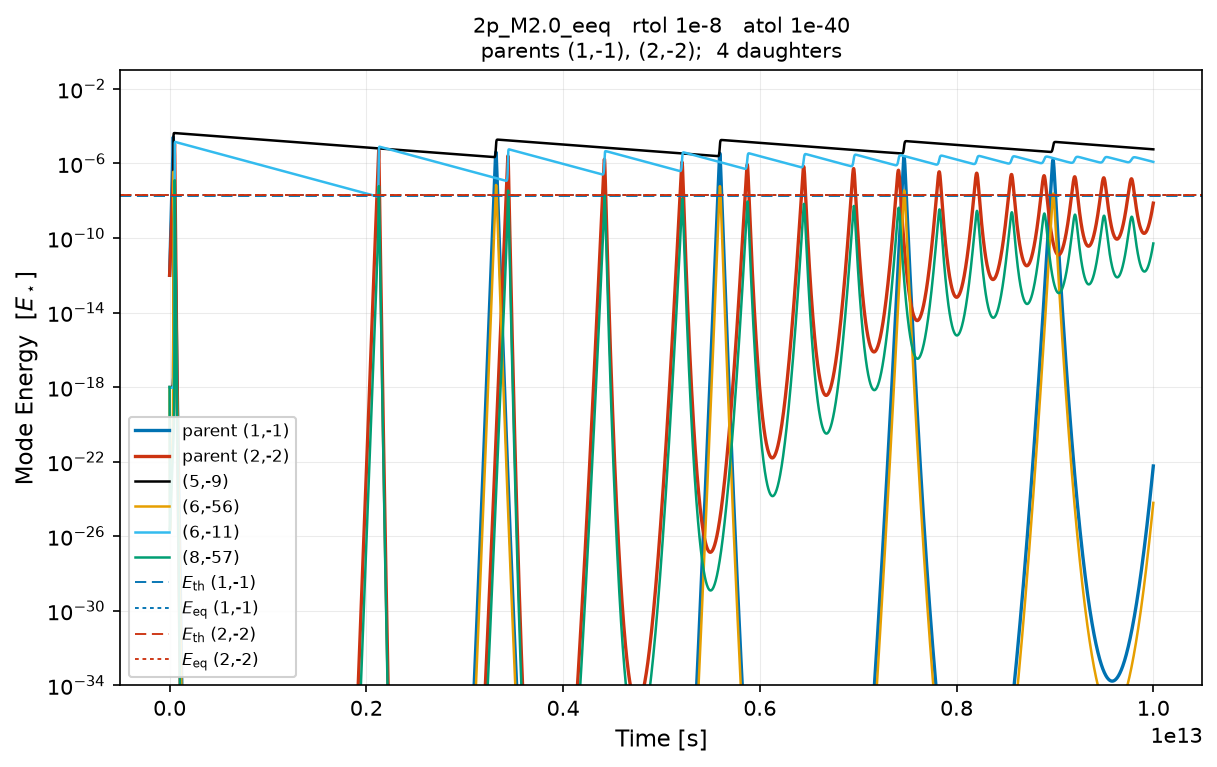
\includegraphics[width=0.21\textwidth,height=0.1323\textwidth]{../plots/rk8pd/2p_M2.0_eeq/r1e-8_a1e-40.png} & 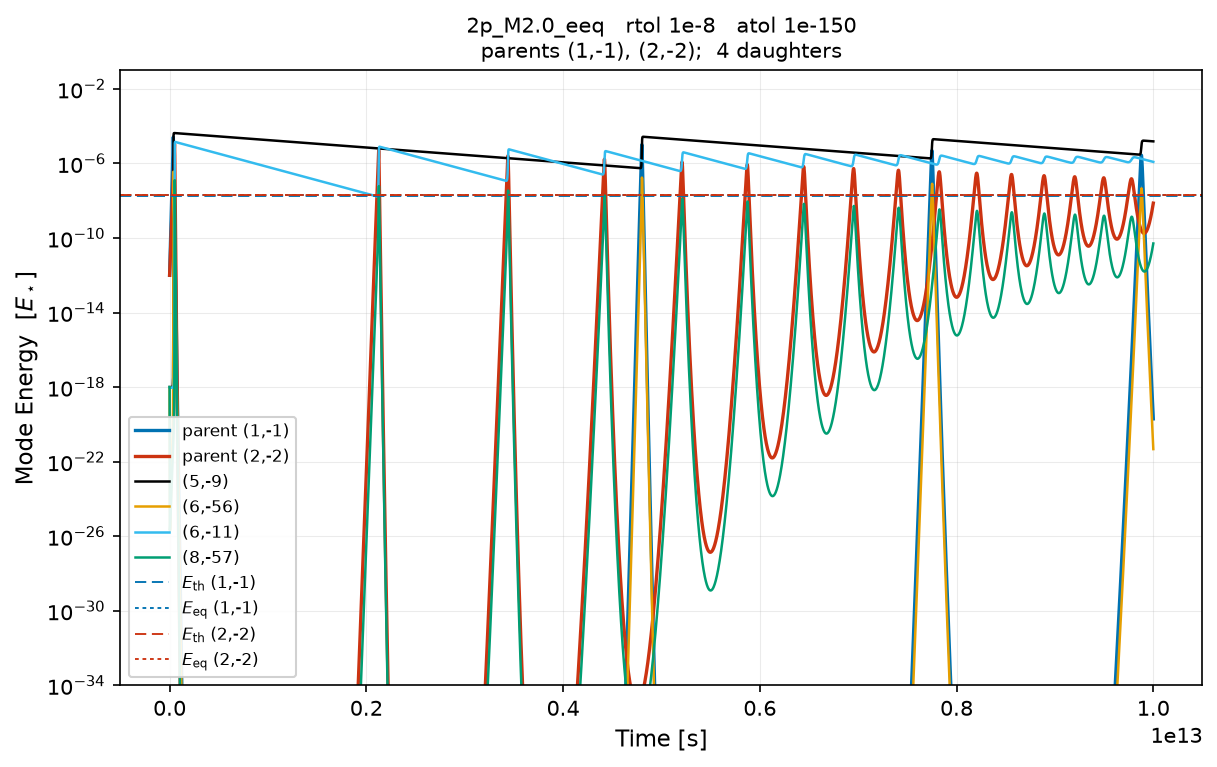
\includegraphics[width=0.21\textwidth,height=0.1323\textwidth]{../plots/rk8pd/2p_M2.0_eeq/r1e-8_a1e-150.png} & 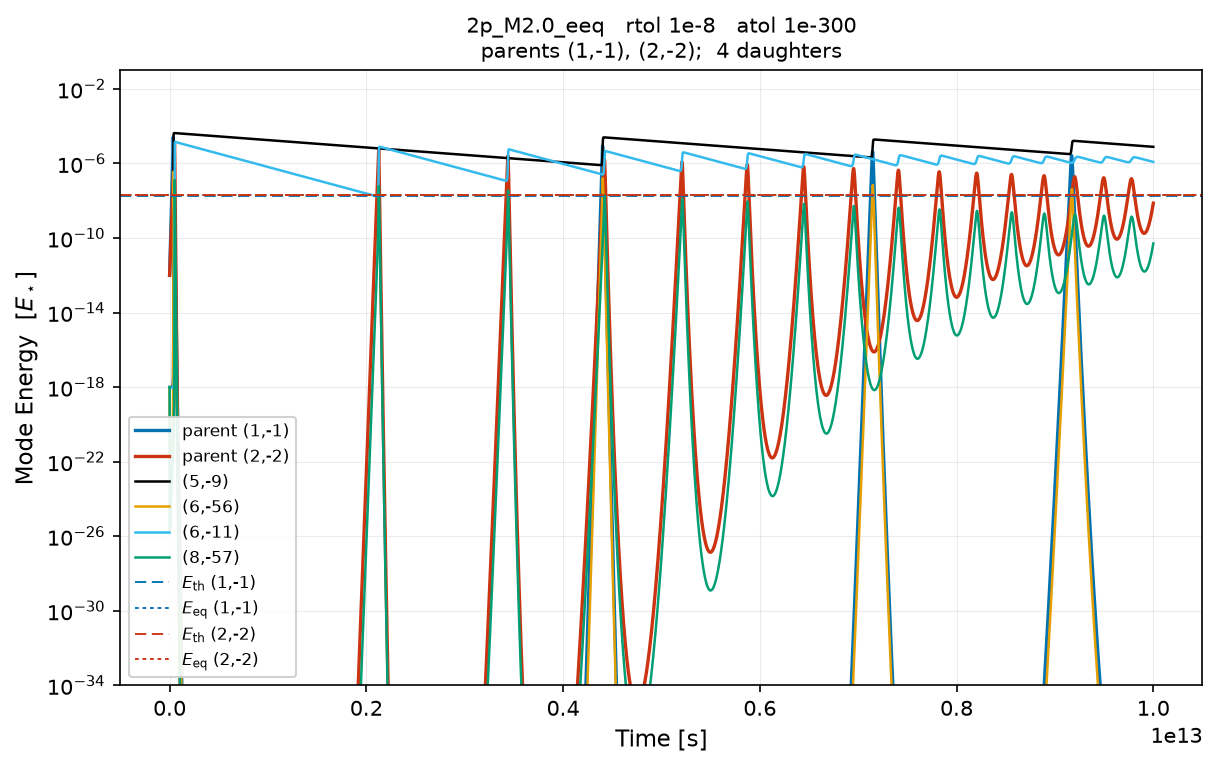
\includegraphics[width=0.21\textwidth,height=0.1323\textwidth]{../plots/rk8pd/2p_M2.0_eeq/r1e-8_a1e-300.png} & 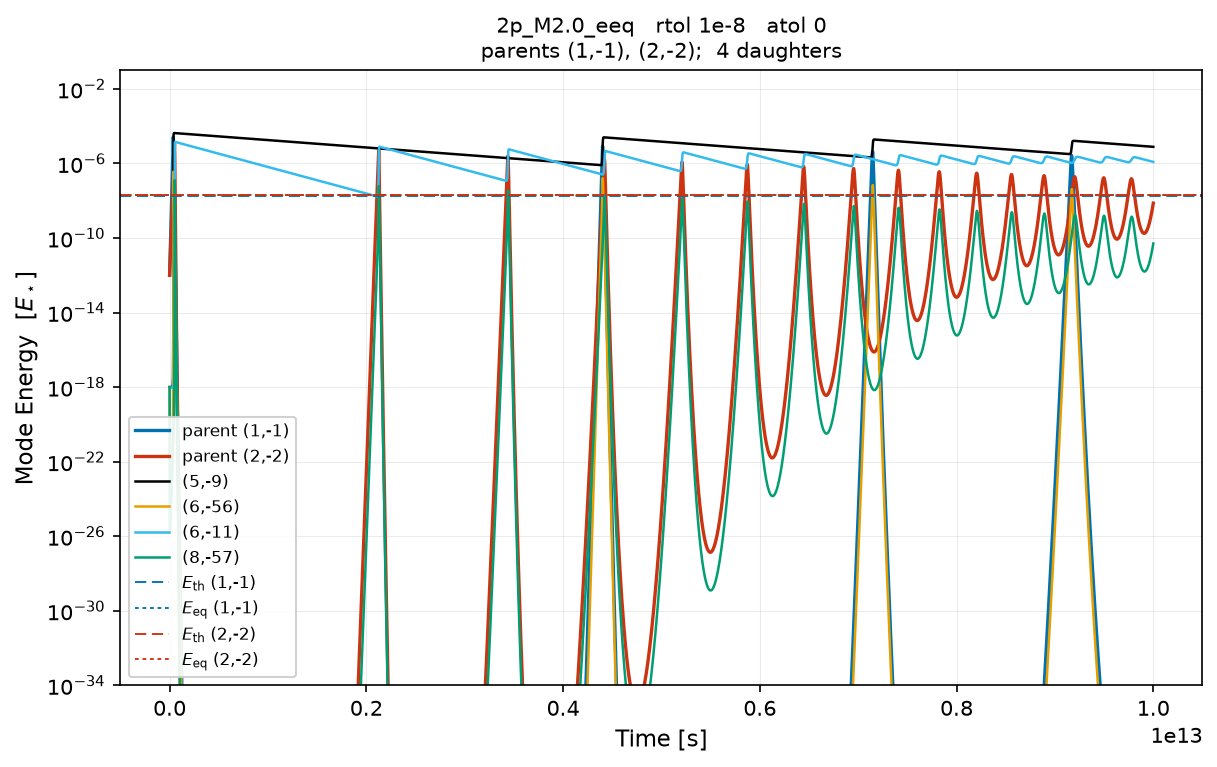
\includegraphics[width=0.21\textwidth,height=0.1323\textwidth]{../plots/rk8pd/2p_M2.0_eeq/r1e-8_a0.png} \\[-1pt]
 & \parbox[t]{0.21\textwidth}{\centering\scriptsize 6.11\,M steps, 16.3\,s} & \parbox[t]{0.21\textwidth}{\centering\scriptsize 8.12\,M steps, 35.2\,s} & \parbox[t]{0.21\textwidth}{\centering\scriptsize 9.27\,M steps, 35.6\,s} & \parbox[t]{0.21\textwidth}{\centering\scriptsize 9.27\,M steps, 32.1\,s} \\[2pt]
\rotatebox{90}{\parbox{0.1323\textwidth}{\centering\scriptsize\bfseries BDF, dense analytic Jacobian}} & 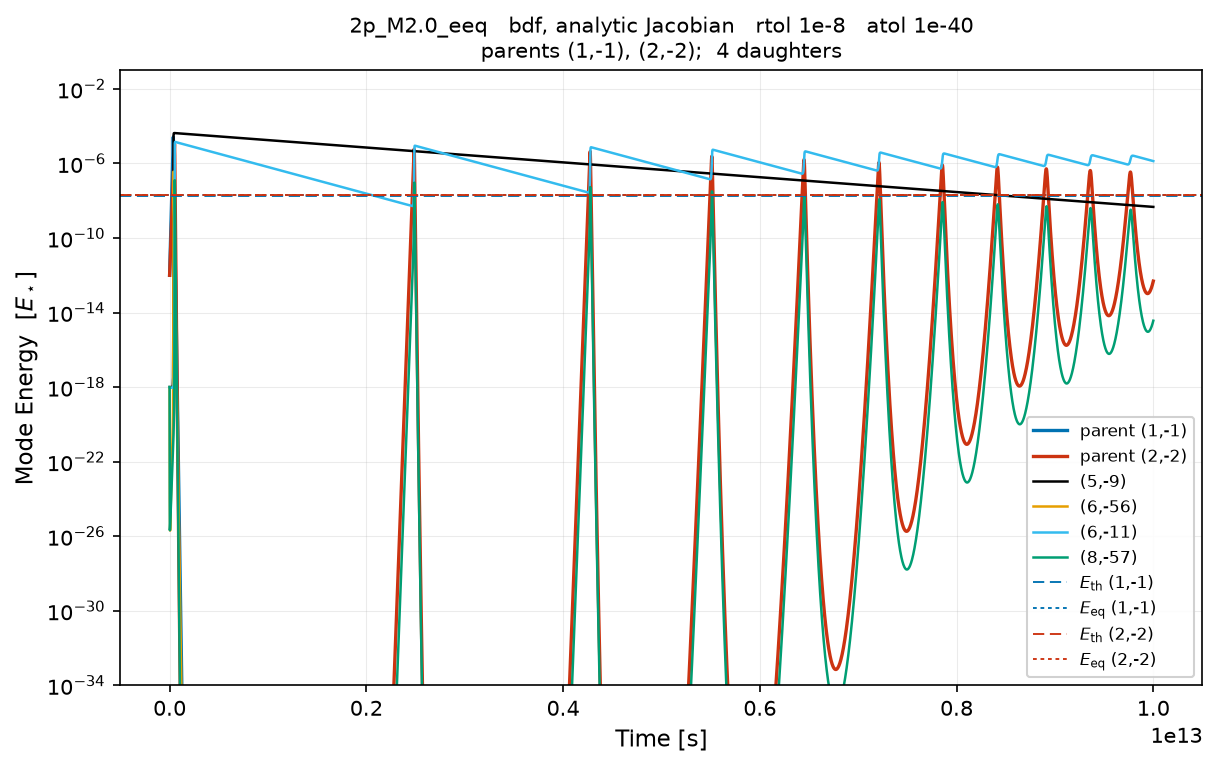
\includegraphics[width=0.21\textwidth,height=0.1323\textwidth]{../plots/bdf/2p_M2.0_eeq/r1e-8_a1e-40.png} & 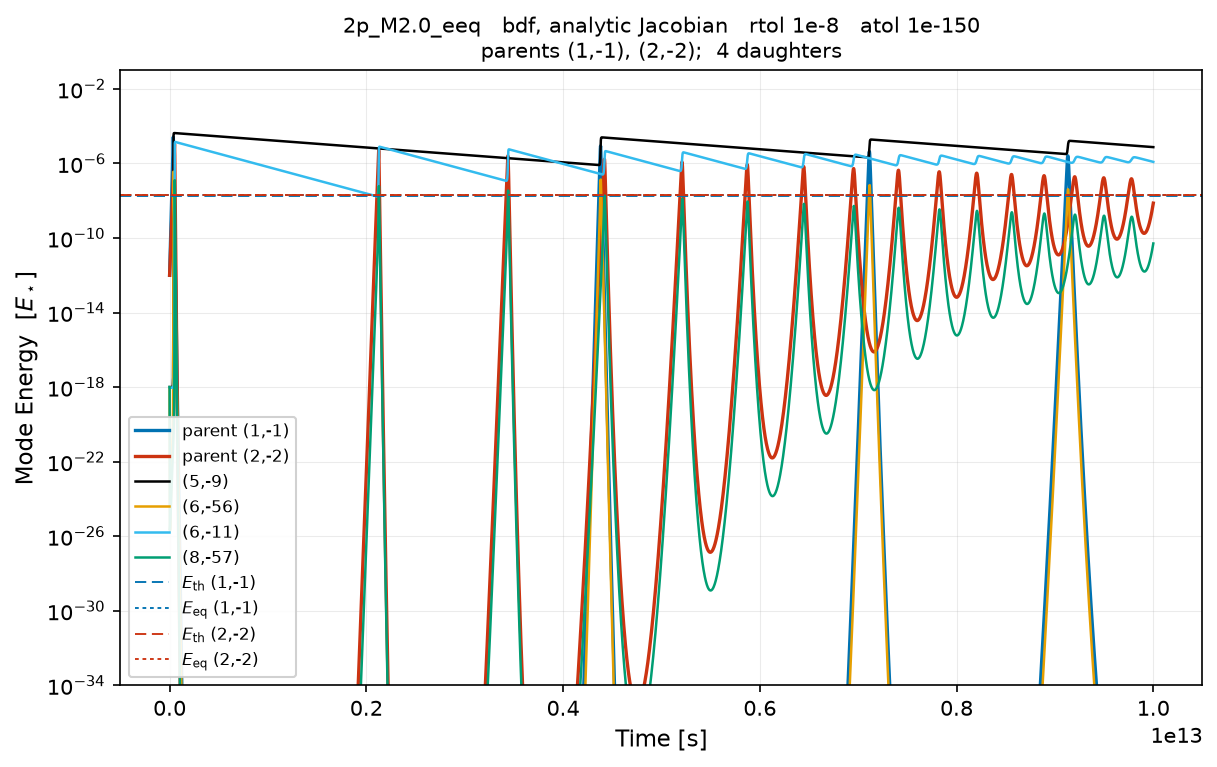
\includegraphics[width=0.21\textwidth,height=0.1323\textwidth]{../plots/bdf/2p_M2.0_eeq/r1e-8_a1e-150.png} & 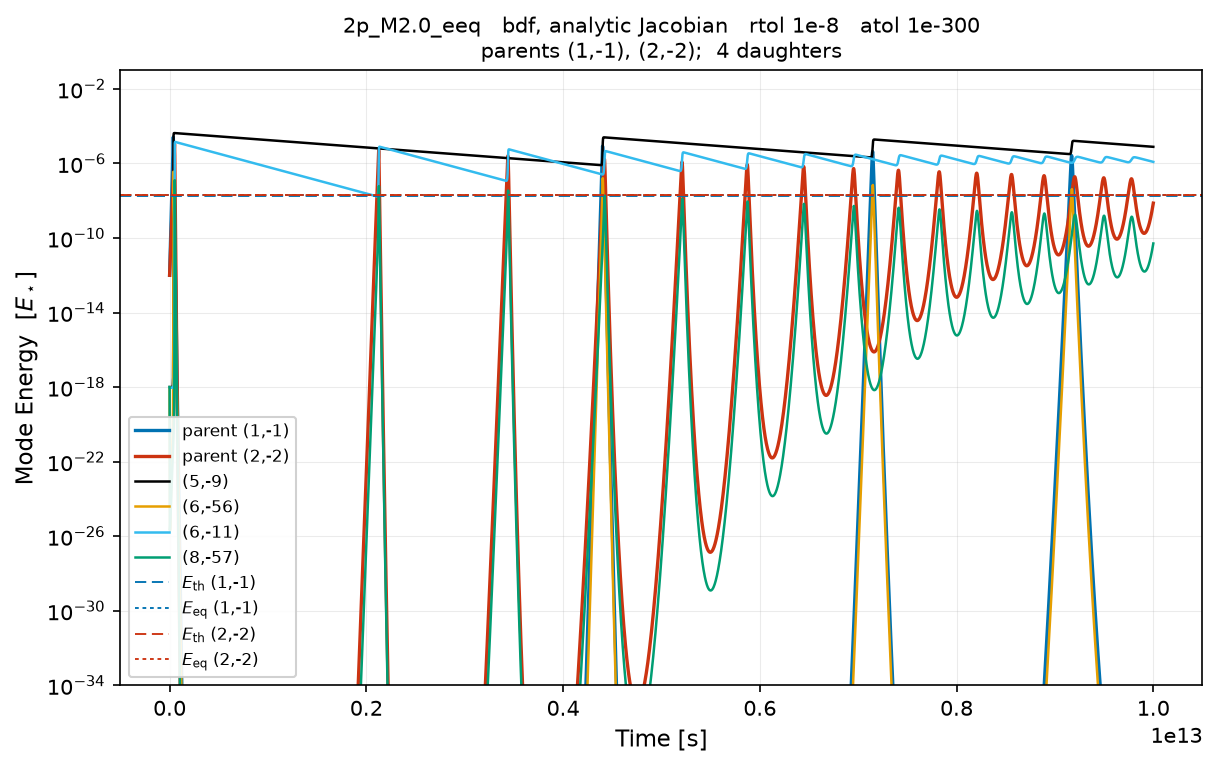
\includegraphics[width=0.21\textwidth,height=0.1323\textwidth]{../plots/bdf/2p_M2.0_eeq/r1e-8_a1e-300.png} & 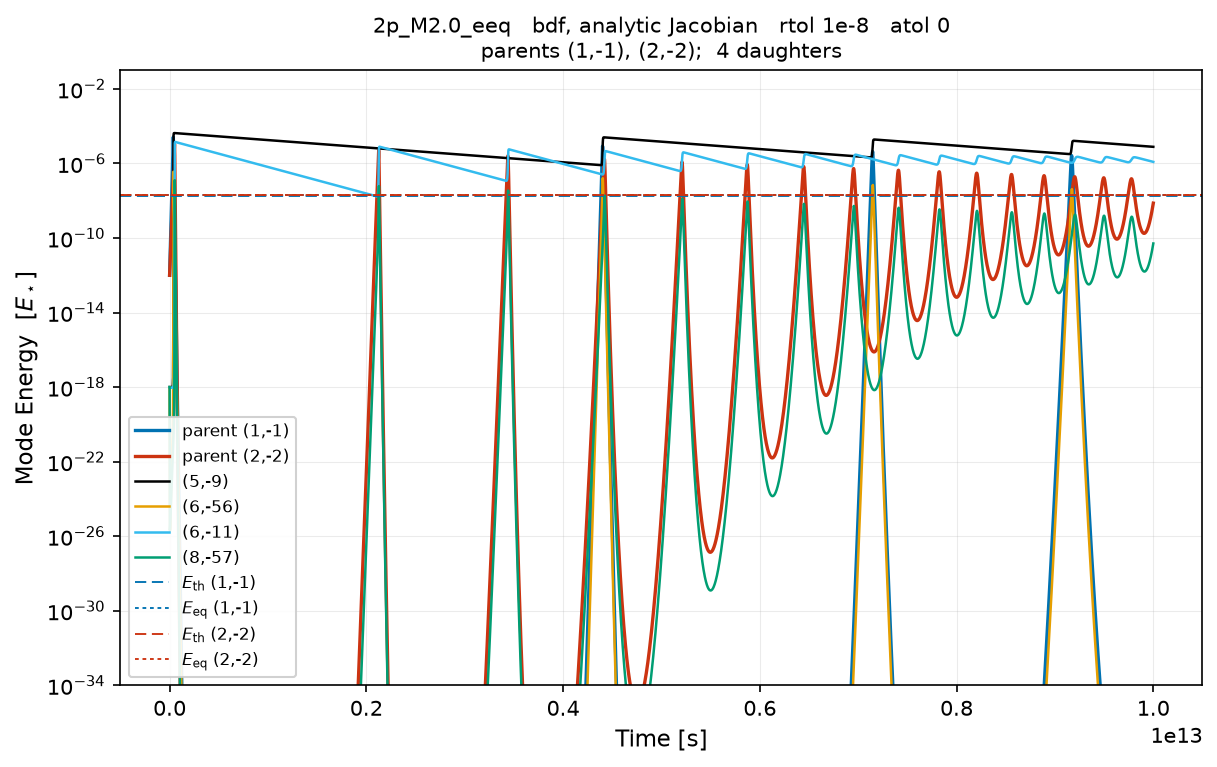
\includegraphics[width=0.21\textwidth,height=0.1323\textwidth]{../plots/bdf/2p_M2.0_eeq/r1e-8_a0.png} \\[-1pt]
 & \parbox[t]{0.21\textwidth}{\centering\scriptsize 18.35\,M steps, 102.8\,s} & \parbox[t]{0.21\textwidth}{\centering\scriptsize 107.34\,M steps, 157.1\,s} & \parbox[t]{0.21\textwidth}{\centering\scriptsize 114.65\,M steps, 193.2\,s} & \parbox[t]{0.21\textwidth}{\centering\scriptsize 114.65\,M steps, 183.6\,s} \\[2pt]
\rotatebox{90}{\parbox{0.1323\textwidth}{\centering\scriptsize\bfseries BDF-Krylov, band full}} & 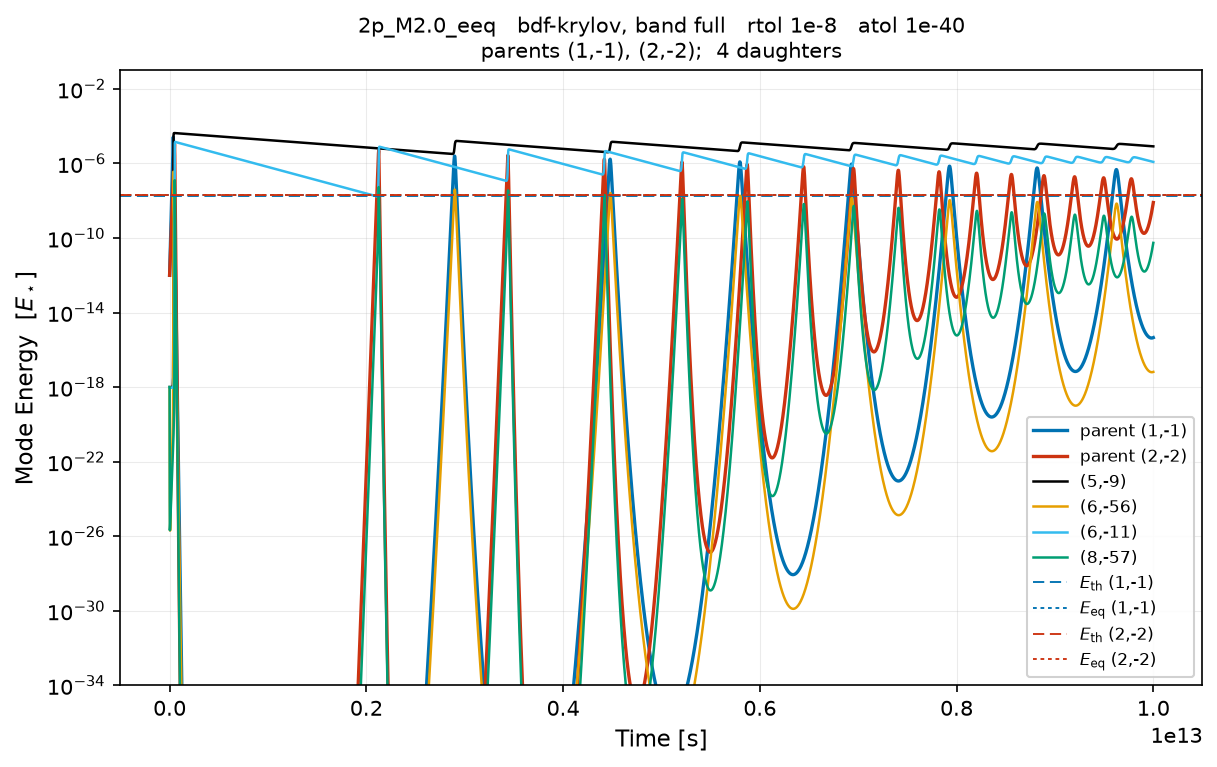
\includegraphics[width=0.21\textwidth,height=0.1323\textwidth]{../plots/krylov_full/2p_M2.0_eeq/r1e-8_a1e-40.png} & 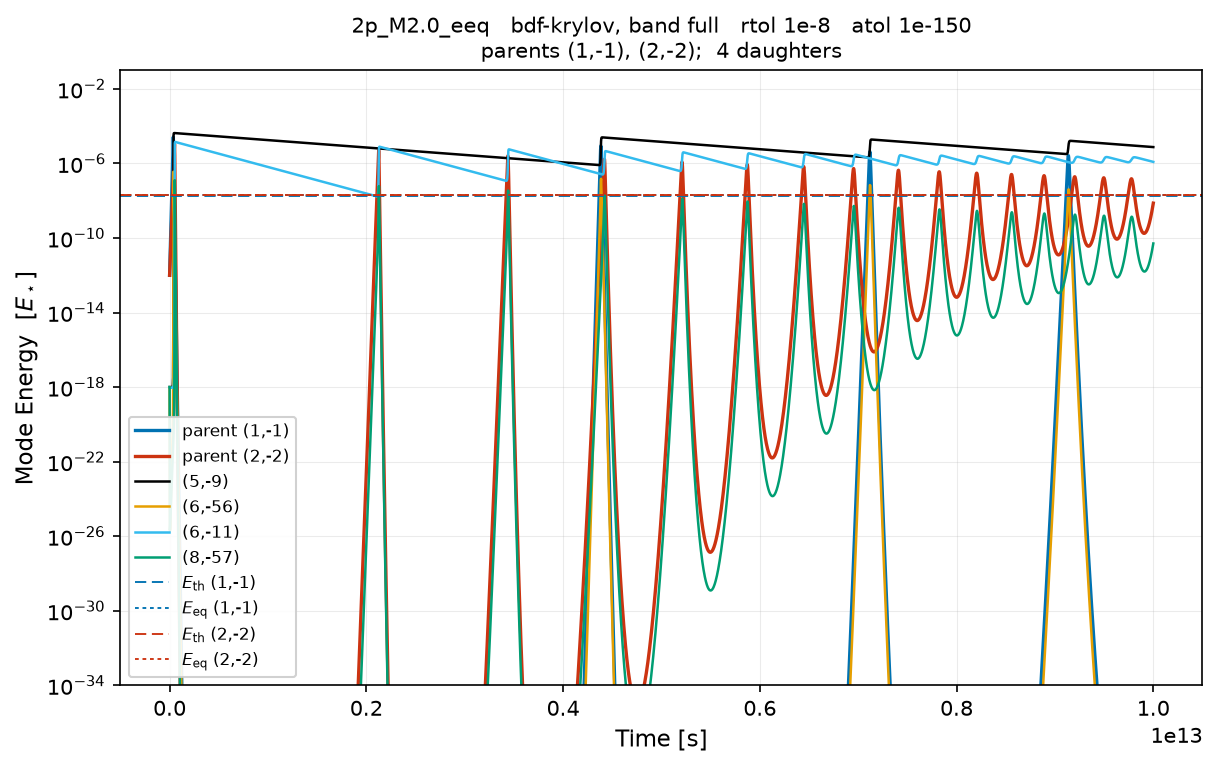
\includegraphics[width=0.21\textwidth,height=0.1323\textwidth]{../plots/krylov_full/2p_M2.0_eeq/r1e-8_a1e-150.png} & 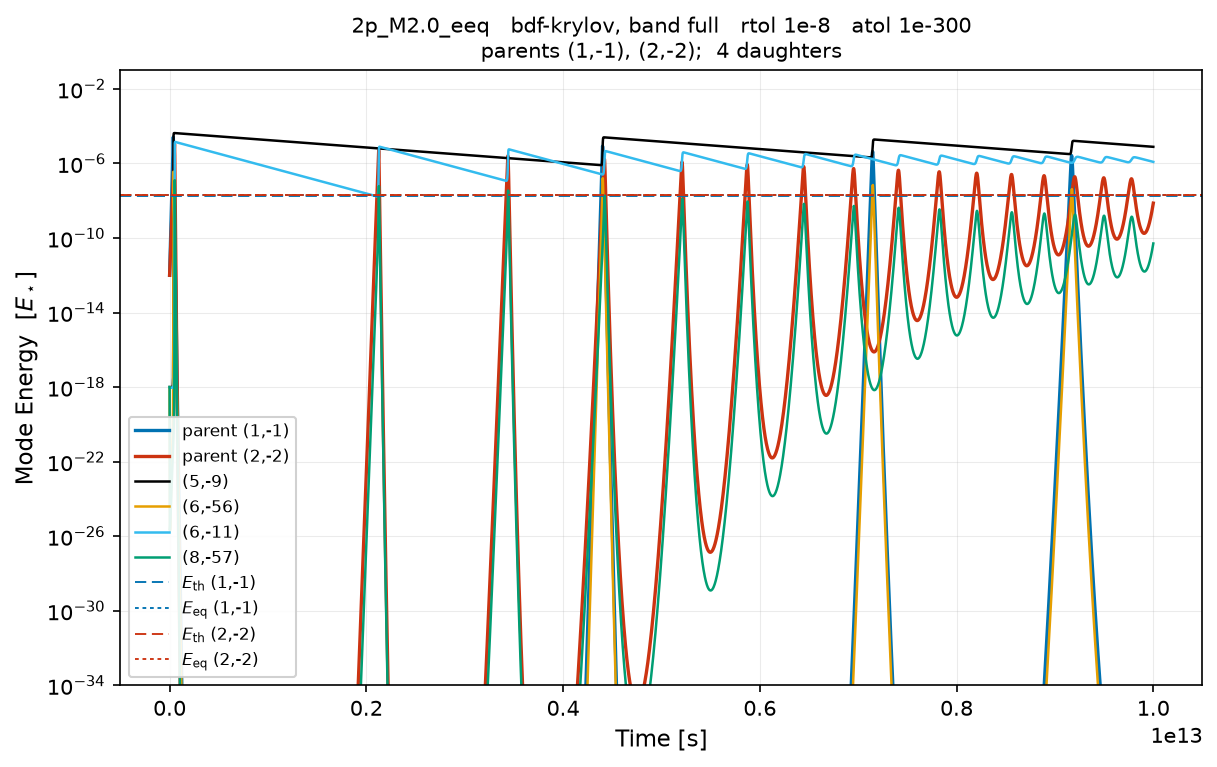
\includegraphics[width=0.21\textwidth,height=0.1323\textwidth]{../plots/krylov_full/2p_M2.0_eeq/r1e-8_a1e-300.png} & 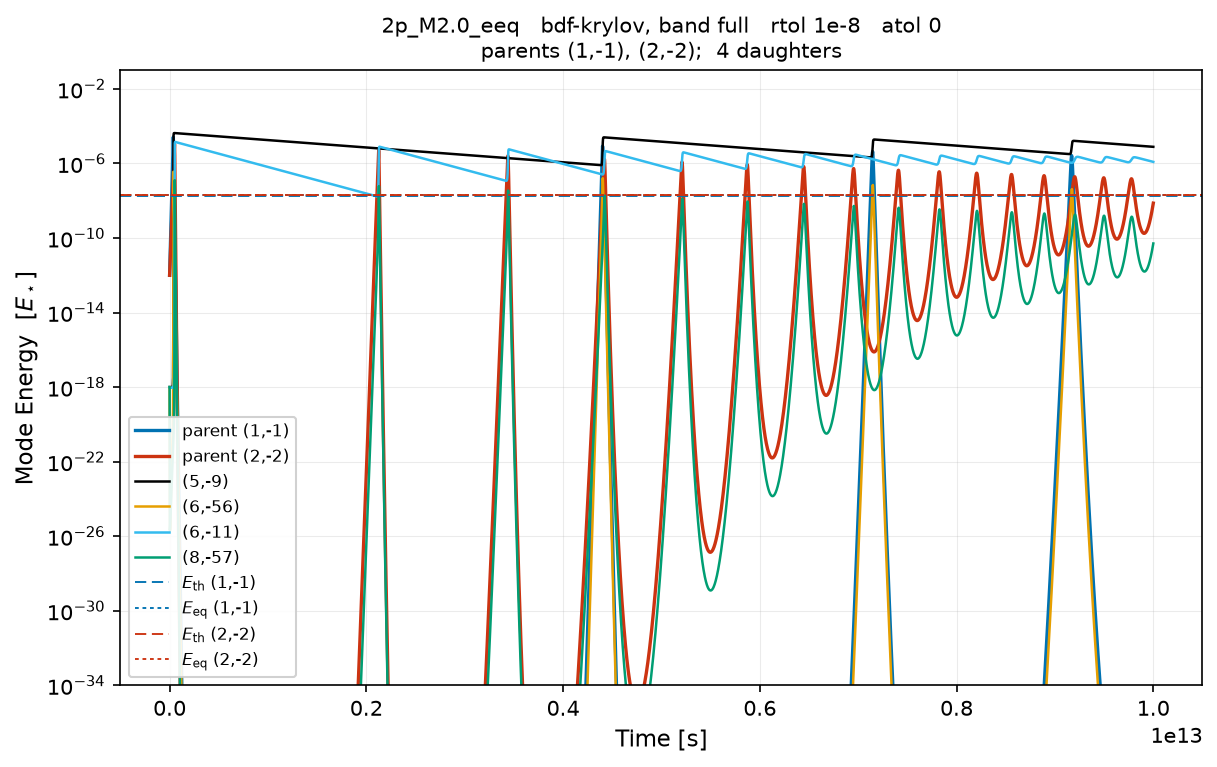
\includegraphics[width=0.21\textwidth,height=0.1323\textwidth]{../plots/krylov_full/2p_M2.0_eeq/r1e-8_a0.png} \\[-1pt]
 & \parbox[t]{0.21\textwidth}{\centering\scriptsize 94.11\,M steps, 215.5\,s} & \parbox[t]{0.21\textwidth}{\centering\scriptsize 103.74\,M steps, 217.1\,s} & \parbox[t]{0.21\textwidth}{\centering\scriptsize 110.66\,M steps, 213.7\,s} & \parbox[t]{0.21\textwidth}{\centering\scriptsize 110.66\,M steps, 219.8\,s} \\[2pt]
\rotatebox{90}{\parbox{0.1323\textwidth}{\centering\scriptsize\bfseries BDF-Krylov, band 3}} & 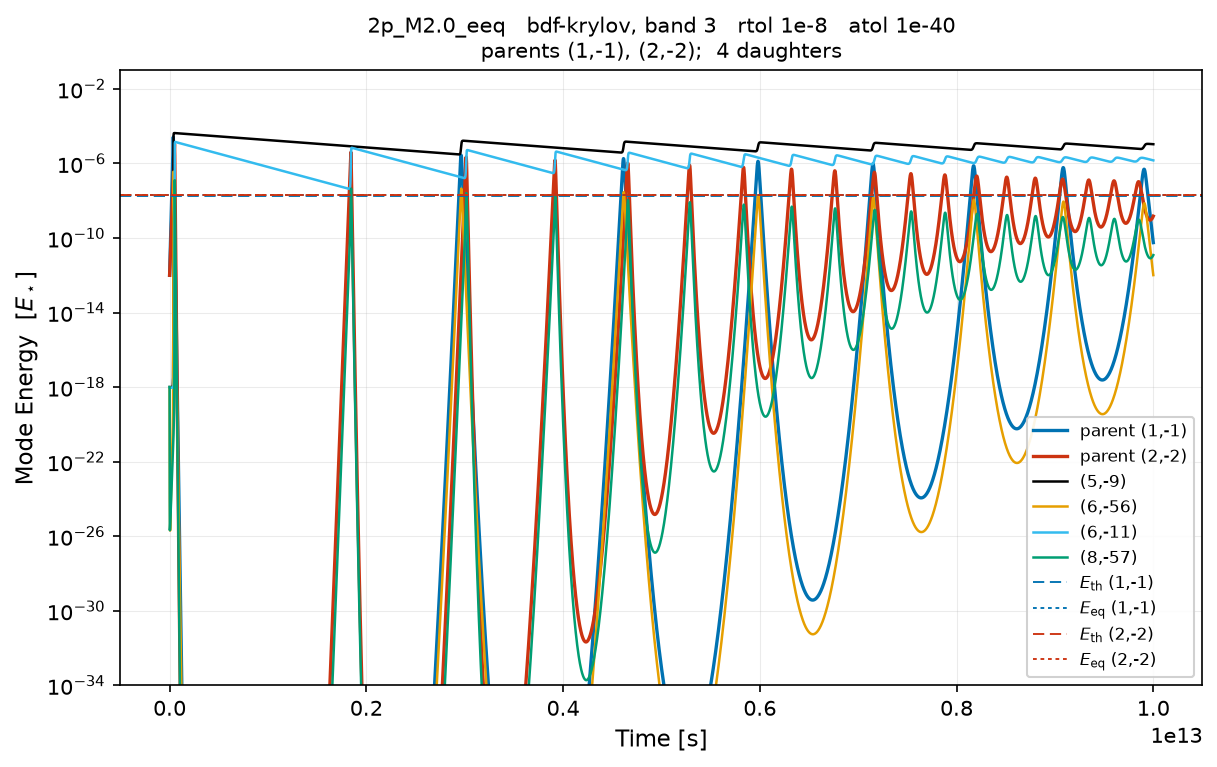
\includegraphics[width=0.21\textwidth,height=0.1323\textwidth]{../plots/krylov_b3/2p_M2.0_eeq/r1e-8_a1e-40.png} & 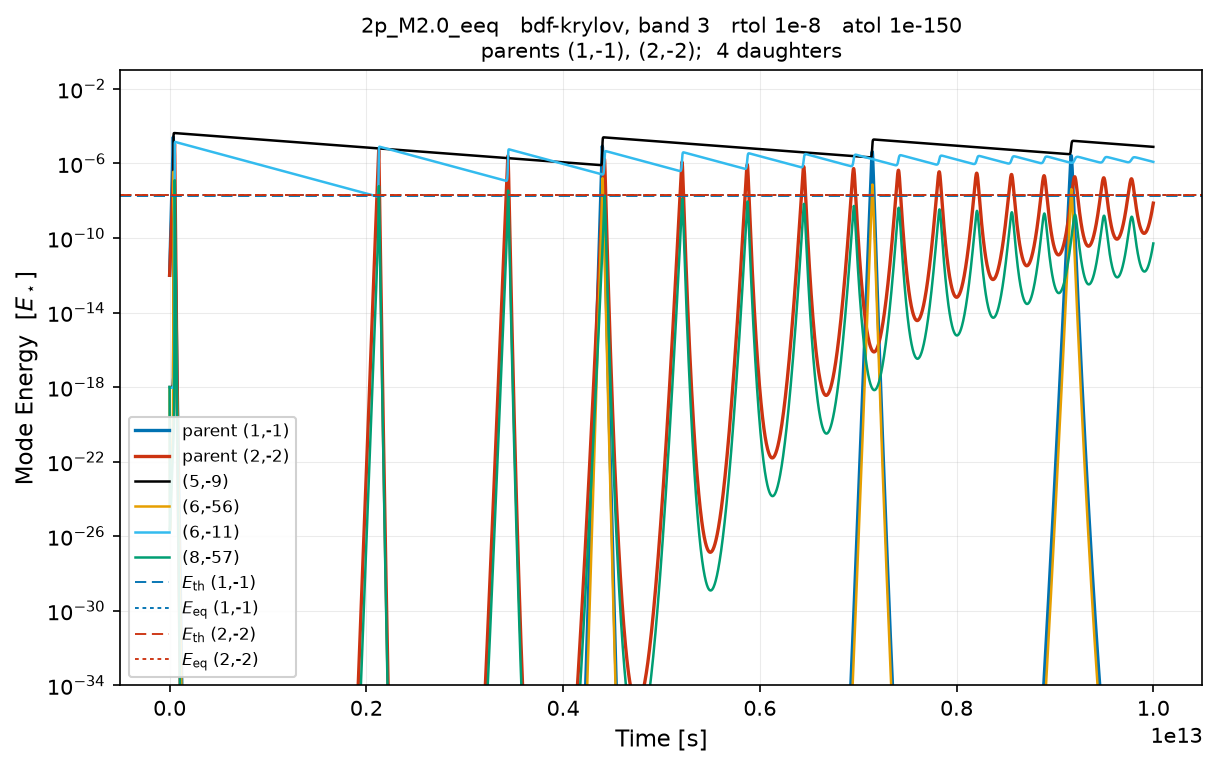
\includegraphics[width=0.21\textwidth,height=0.1323\textwidth]{../plots/krylov_b3/2p_M2.0_eeq/r1e-8_a1e-150.png} & 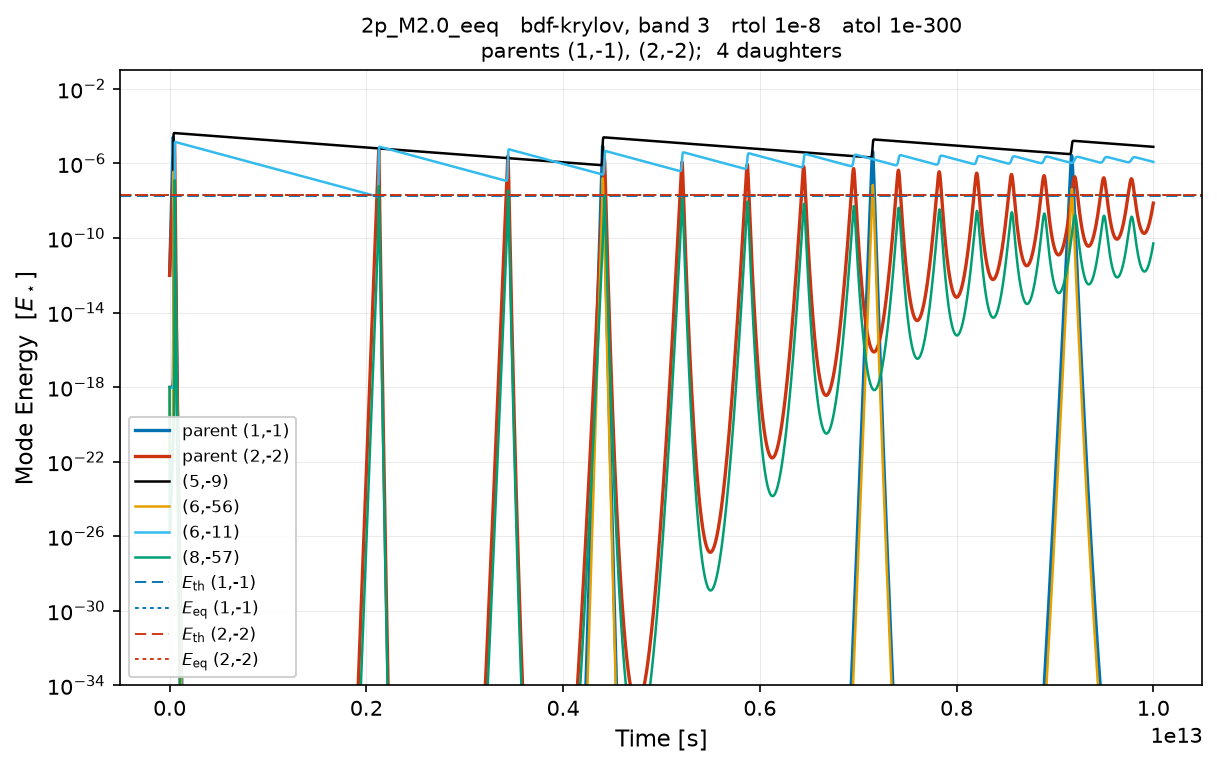
\includegraphics[width=0.21\textwidth,height=0.1323\textwidth]{../plots/krylov_b3/2p_M2.0_eeq/r1e-8_a1e-300.png} & 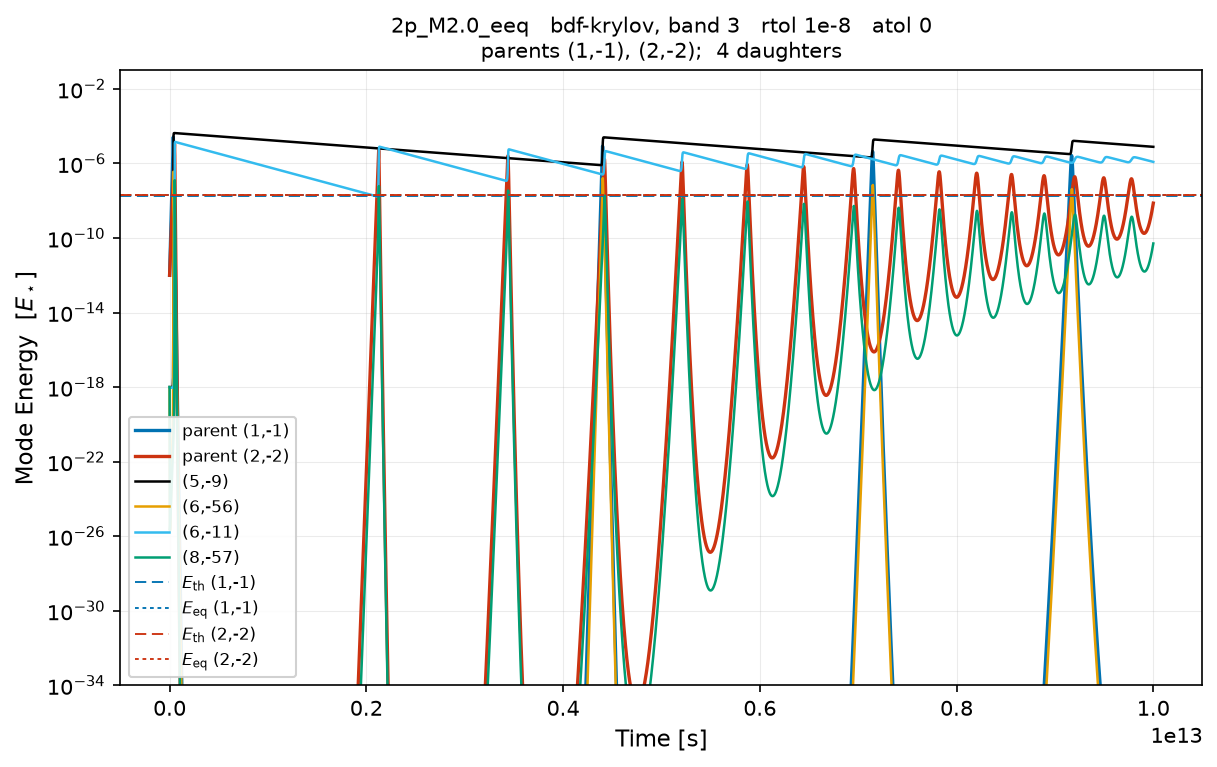
\includegraphics[width=0.21\textwidth,height=0.1323\textwidth]{../plots/krylov_b3/2p_M2.0_eeq/r1e-8_a0.png} \\[-1pt]
 & \parbox[t]{0.21\textwidth}{\centering\scriptsize 88.88\,M steps, 156.9\,s} & \parbox[t]{0.21\textwidth}{\centering\scriptsize 99.22\,M steps, 218.3\,s} & \parbox[t]{0.21\textwidth}{\centering\scriptsize 106.40\,M steps, 277.2\,s} & \parbox[t]{0.21\textwidth}{\centering\scriptsize 106.40\,M steps, 219.0\,s} \\[2pt]
\rotatebox{90}{\parbox{0.1323\textwidth}{\centering\scriptsize\bfseries Adams, fixed point}} & 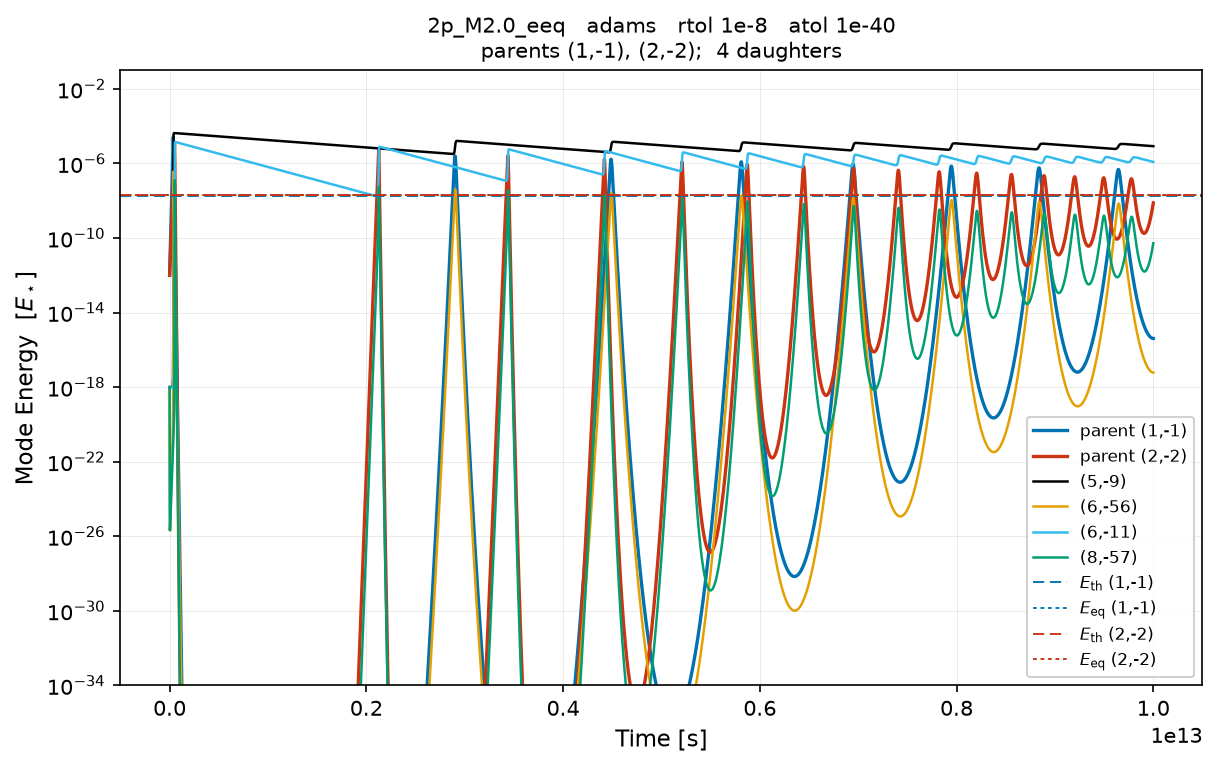
\includegraphics[width=0.21\textwidth,height=0.1323\textwidth]{../plots/adams/2p_M2.0_eeq/r1e-8_a1e-40.png} & 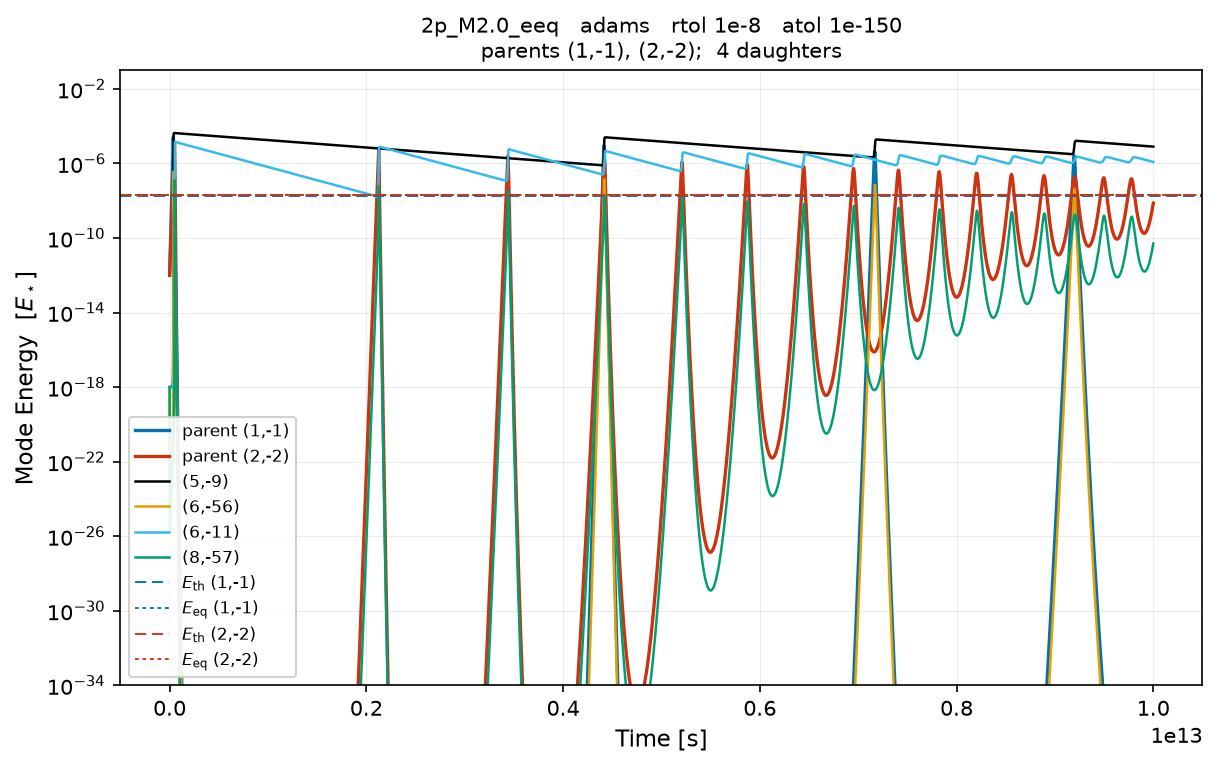
\includegraphics[width=0.21\textwidth,height=0.1323\textwidth]{../plots/adams/2p_M2.0_eeq/r1e-8_a1e-150.png} & 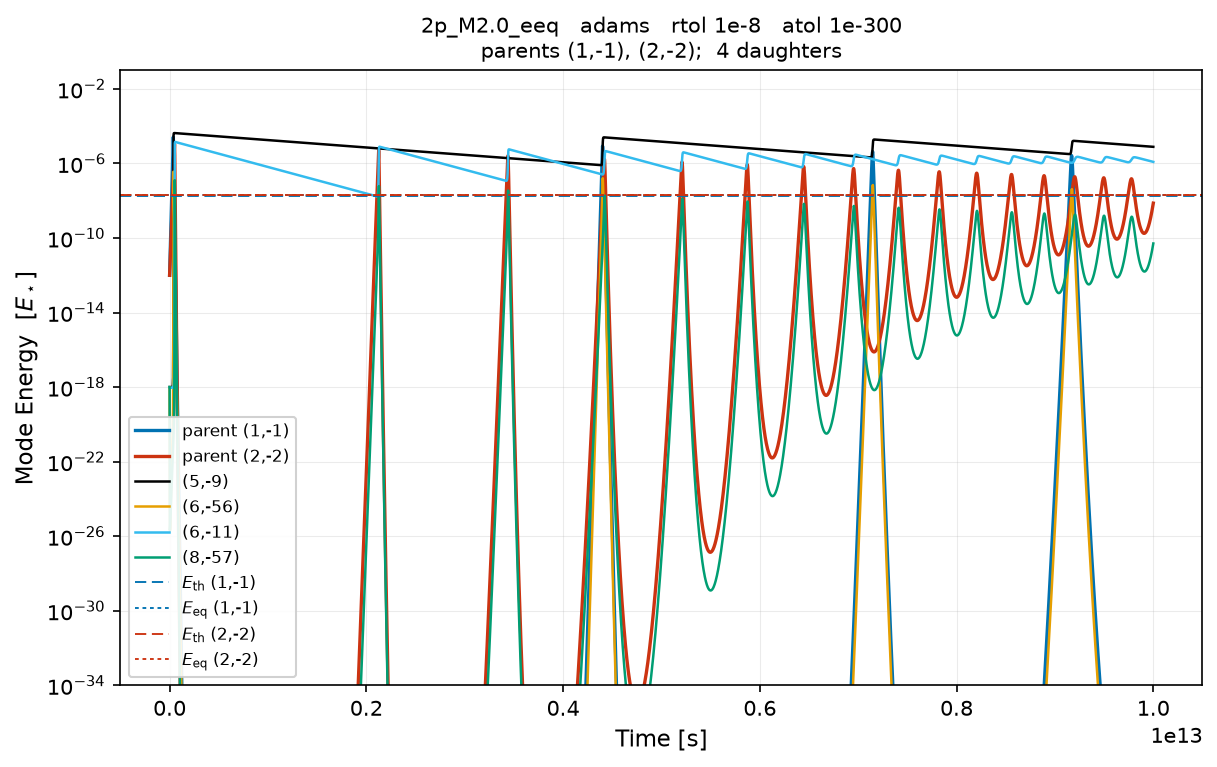
\includegraphics[width=0.21\textwidth,height=0.1323\textwidth]{../plots/adams/2p_M2.0_eeq/r1e-8_a1e-300.png} & 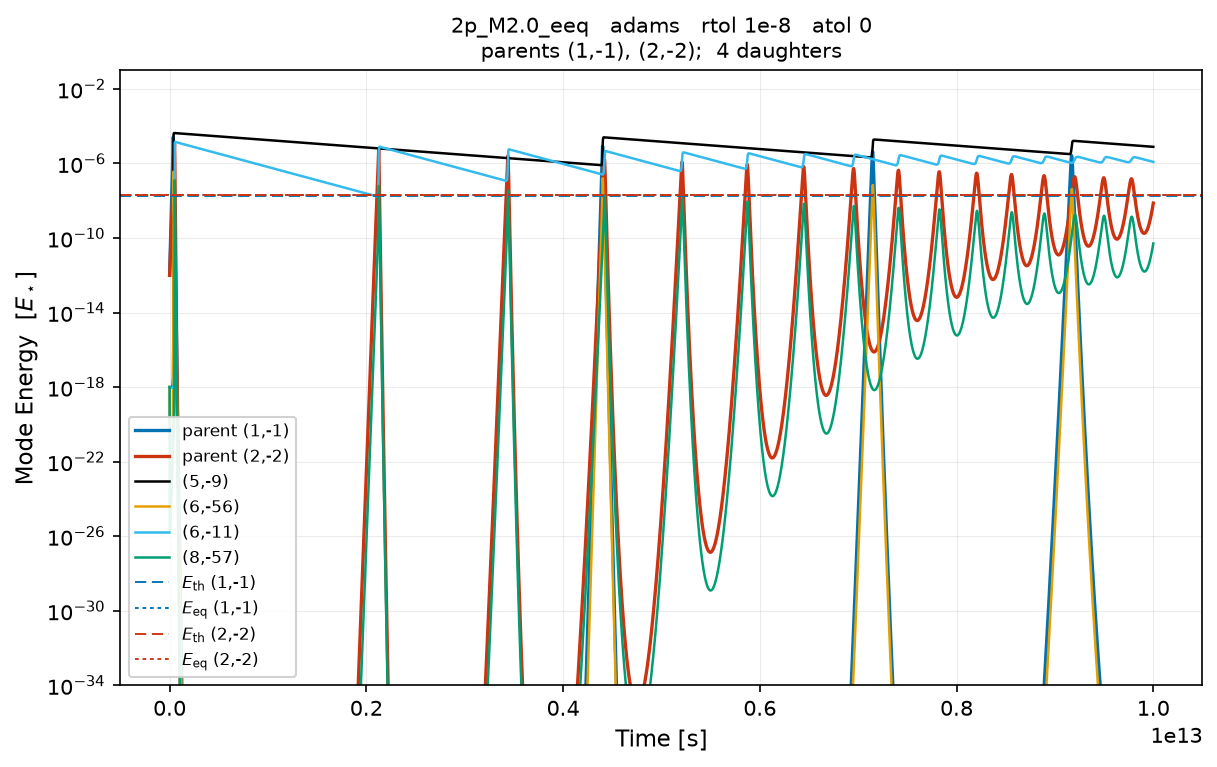
\includegraphics[width=0.21\textwidth,height=0.1323\textwidth]{../plots/adams/2p_M2.0_eeq/r1e-8_a0.png} \\[-1pt]
 & \parbox[t]{0.21\textwidth}{\centering\scriptsize 40.39\,M steps, 52.7\,s} & \parbox[t]{0.21\textwidth}{\centering\scriptsize 43.82\,M steps, 57.0\,s} & \parbox[t]{0.21\textwidth}{\centering\scriptsize 46.13\,M steps, 49.8\,s} & \parbox[t]{0.21\textwidth}{\centering\scriptsize 46.13\,M steps, 48.4\,s} \\[2pt]
\end{tabular}\par}
\par\noindent{\scriptsize\setlength\tabcolsep{3.5pt}\renewcommand\arraystretch{0.92}
\begin{tabular}{@{}llllrrrrrrr@{}}
\toprule
integrator & atol & stop & $t_{\rm stop}$ [s] & steps & rejected & RHS & Jac. & NL it. & lin. it. & wall [s] \\
\midrule
rk8pd & $10^{-40}$ & end & $1.00\times10^{13}$ & 6.11\,M & 535.4\,k & 79.40\,M & -- & -- & -- & 16.3 \\
 & $10^{-150}$ & end & $1.00\times10^{13}$ & 8.12\,M & 944.9\,k & 105.61\,M & -- & -- & -- & 35.2 \\
 & $10^{-300}$ & end & $1.00\times10^{13}$ & 9.27\,M & 1.04\,M & 120.46\,M & -- & -- & -- & 35.6 \\
 & $0$ & end & $1.00\times10^{13}$ & 9.27\,M & 1.04\,M & 120.46\,M & -- & -- & -- & 32.1 \\
\addlinespace[2pt]
BDF, dense analytic Jacobian & $10^{-40}$ & end & $1.00\times10^{13}$ & 18.35\,M & 206.2\,k & 20.00\,M & 382.9\,k & 20.00\,M & -- & 102.8 \\
 & $10^{-150}$ & end & $1.00\times10^{13}$ & 107.34\,M & 674.9\,k & 113.72\,M & 1.81\,M & 113.72\,M & -- & 157.1 \\
 & $10^{-300}$ & end & $1.00\times10^{13}$ & 114.65\,M & 735.3\,k & 121.52\,M & 1.93\,M & 121.52\,M & -- & 193.2 \\
 & $0$ & end & $1.00\times10^{13}$ & 114.65\,M & 735.3\,k & 121.52\,M & 1.93\,M & 121.52\,M & -- & 183.6 \\
\addlinespace[2pt]
BDF-Krylov, band full & $10^{-40}$ & end & $1.00\times10^{13}$ & 94.11\,M & 669.5\,k & 220.88\,M & 1.58\,M & 100.68\,M & 101.20\,M & 215.5 \\
 & $10^{-150}$ & end & $1.00\times10^{13}$ & 103.74\,M & 765.1\,k & 239.23\,M & 1.74\,M & 110.95\,M & 107.36\,M & 217.1 \\
 & $10^{-300}$ & end & $1.00\times10^{13}$ & 110.66\,M & 843.3\,k & 254.79\,M & 1.86\,M & 118.47\,M & 114.00\,M & 213.7 \\
 & $0$ & end & $1.00\times10^{13}$ & 110.66\,M & 843.3\,k & 254.79\,M & 1.86\,M & 118.47\,M & 114.00\,M & 219.8 \\
\addlinespace[2pt]
BDF-Krylov, band 3 & $10^{-40}$ & end & $1.00\times10^{13}$ & 88.88\,M & 917.3\,k & 219.52\,M & 1.50\,M & 96.67\,M & 112.37\,M & 156.9 \\
 & $10^{-150}$ & end & $1.00\times10^{13}$ & 99.22\,M & 1.06\,M & 241.99\,M & 1.67\,M & 107.98\,M & 122.31\,M & 218.3 \\
 & $10^{-300}$ & end & $1.00\times10^{13}$ & 106.40\,M & 1.15\,M & 258.82\,M & 1.79\,M & 115.88\,M & 130.40\,M & 277.2 \\
 & $0$ & end & $1.00\times10^{13}$ & 106.40\,M & 1.15\,M & 258.82\,M & 1.79\,M & 115.88\,M & 130.40\,M & 219.0 \\
\addlinespace[2pt]
Adams, fixed point & $10^{-40}$ & end & $1.00\times10^{13}$ & 40.39\,M & 1.44\,M & 58.85\,M & -- & 58.84\,M & -- & 52.7 \\
 & $10^{-150}$ & end & $1.00\times10^{13}$ & 43.82\,M & 1.91\,M & 64.54\,M & -- & 64.54\,M & -- & 57.0 \\
 & $10^{-300}$ & end & $1.00\times10^{13}$ & 46.13\,M & 2.08\,M & 67.26\,M & -- & 67.26\,M & -- & 49.8 \\
 & $0$ & end & $1.00\times10^{13}$ & 46.13\,M & 2.08\,M & 67.26\,M & -- & 67.26\,M & -- & 48.4 \\
\bottomrule
\end{tabular}}


\appendix
\clearpage
\section{rk8pd: relative tolerance}\label{app:rk8pd}
These pages use the same layout as the network pages, but the rows are $\rtol$ instead of integrators. $\rtol=10^{-10}$ was run only at $\atol=0$ and $10^{-40}$.

\clearpage
\subsection{\texttt{1p2d\_M1.7\_eth}: rk8pd, rtol $\times$ atol}
\noindent See \S\ref{net:1p2d_M1.7_eth} for the network. The second burst disagreed between rk8pd and BDF in the earlier sweep.
\par\smallskip{\centering\begin{tabular}{@{}c@{\hspace{2pt}}c@{\hspace{2pt}}c@{\hspace{2pt}}c@{\hspace{2pt}}c@{}}
 & \small atol $10^{-40}$ & \small atol $10^{-150}$ & \small atol $10^{-300}$ & \small atol $0$ \\[1pt]
\rotatebox{90}{\parbox{0.1323\textwidth}{\centering\scriptsize\bfseries rtol $10^{-8}$}} & 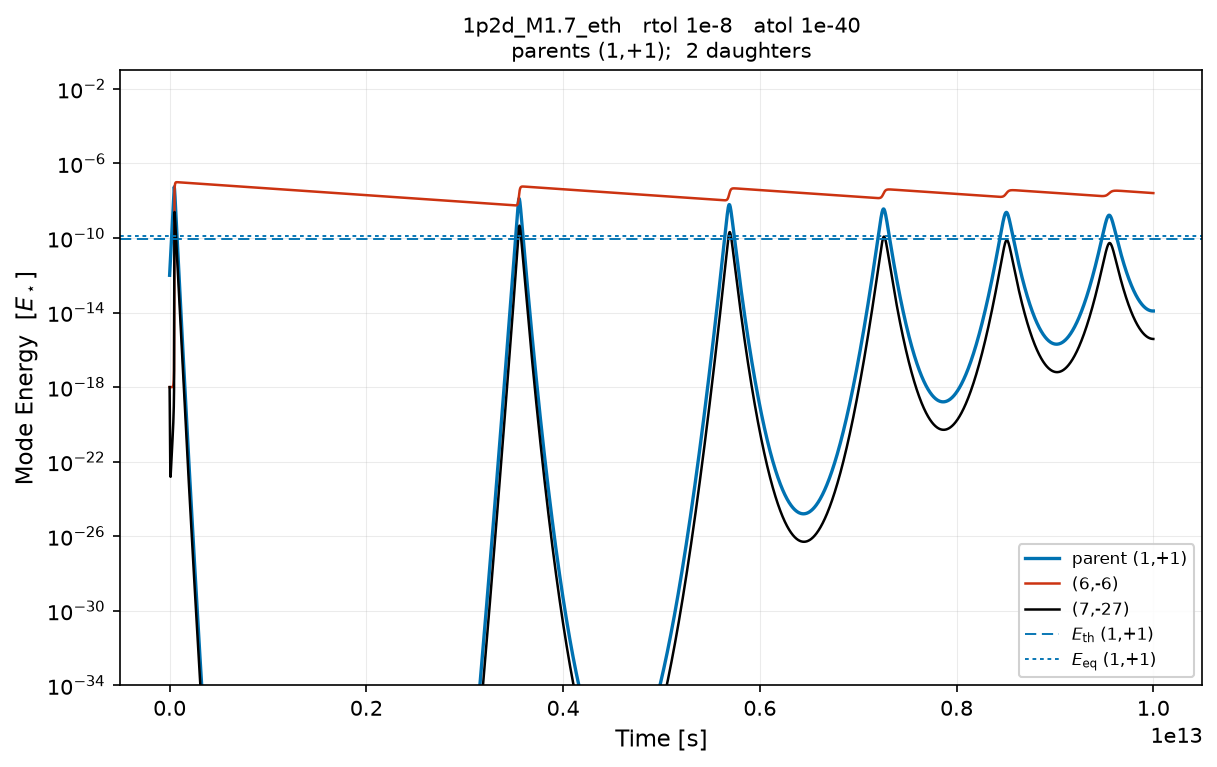
\includegraphics[width=0.21\textwidth,height=0.1323\textwidth]{../plots/rk8pd/1p2d_M1.7_eth/r1e-8_a1e-40.png} & 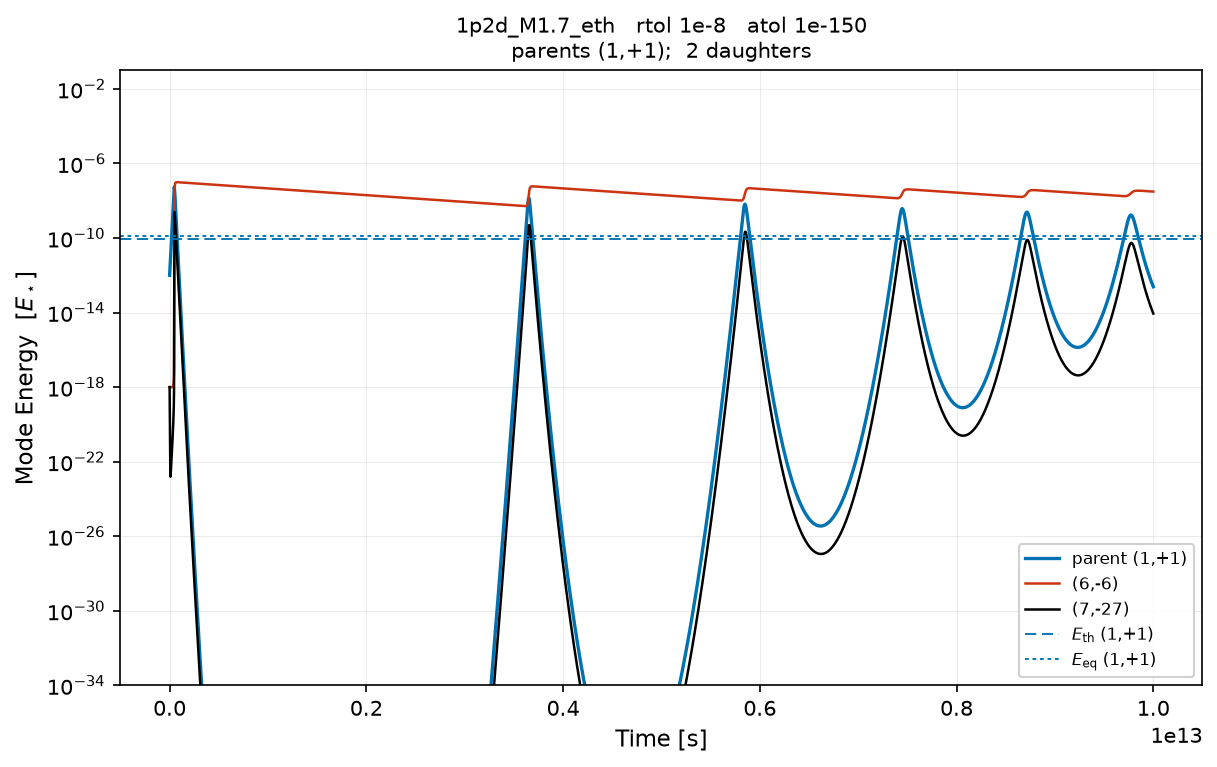
\includegraphics[width=0.21\textwidth,height=0.1323\textwidth]{../plots/rk8pd/1p2d_M1.7_eth/r1e-8_a1e-150.png} & 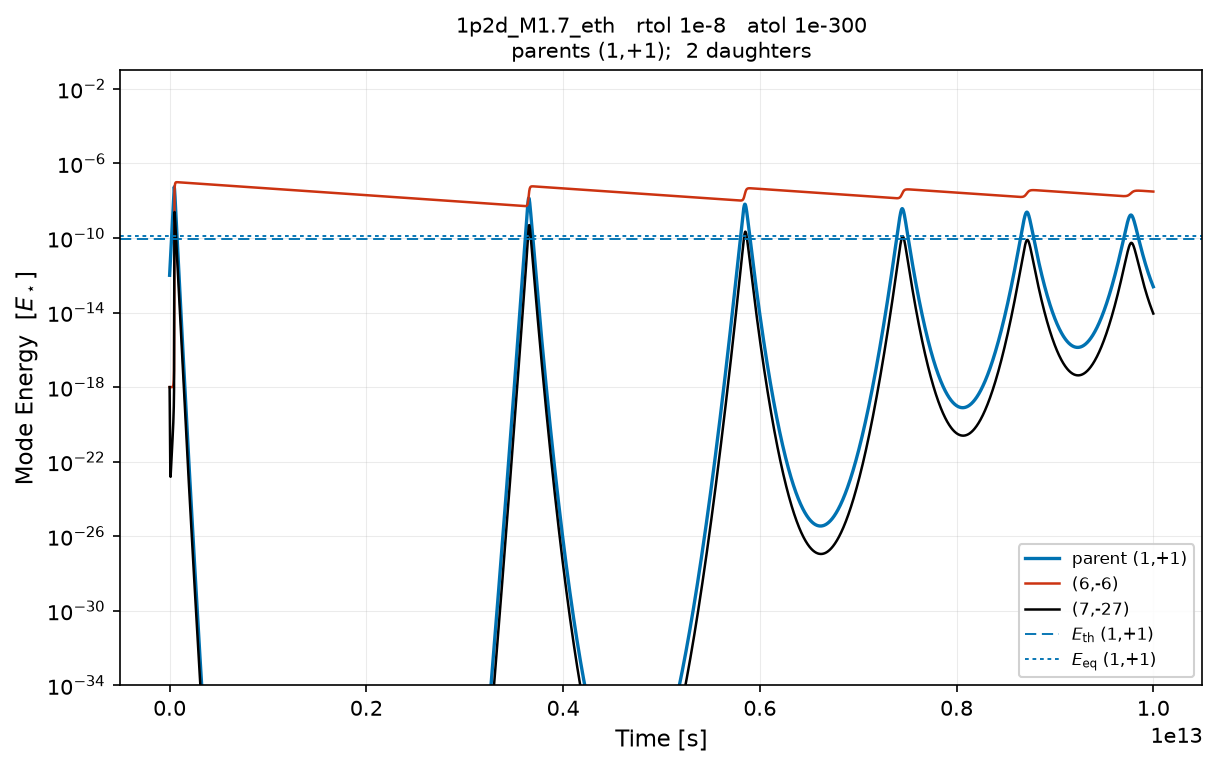
\includegraphics[width=0.21\textwidth,height=0.1323\textwidth]{../plots/rk8pd/1p2d_M1.7_eth/r1e-8_a1e-300.png} & 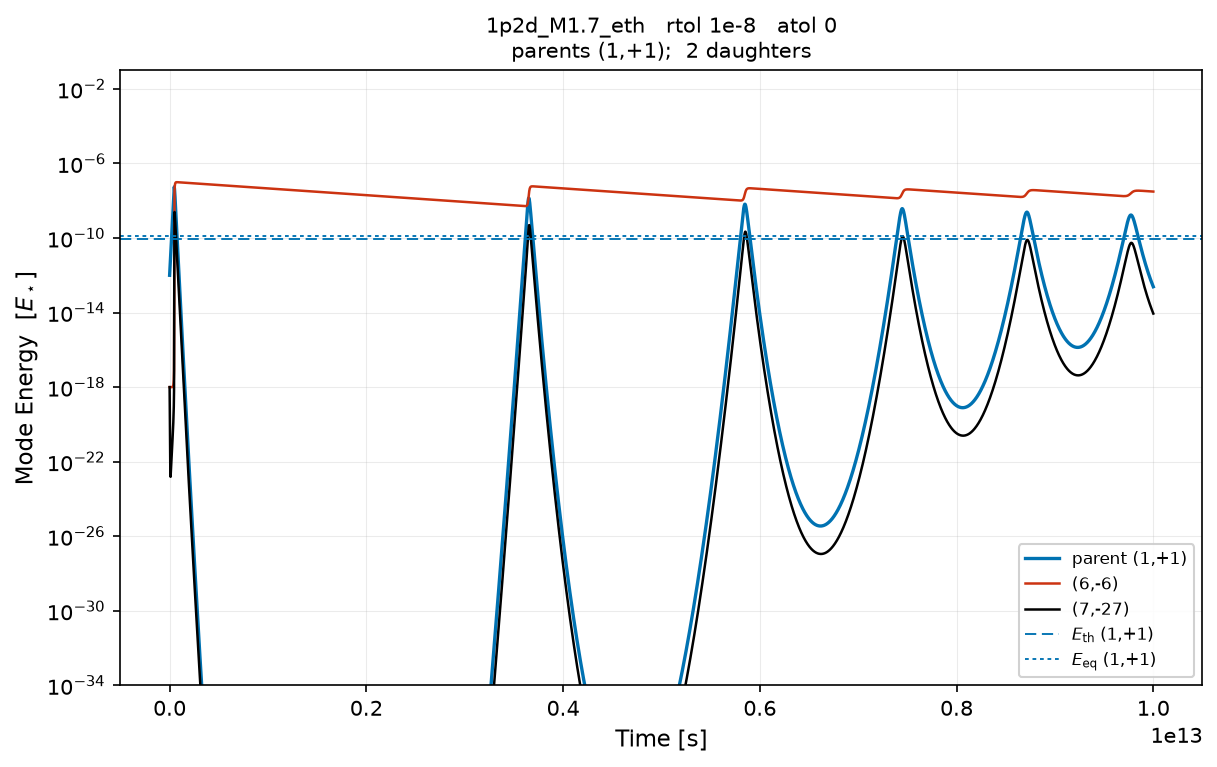
\includegraphics[width=0.21\textwidth,height=0.1323\textwidth]{../plots/rk8pd/1p2d_M1.7_eth/r1e-8_a0.png} \\[-1pt]
 & \parbox[t]{0.21\textwidth}{\centering\scriptsize 953.2\,k steps, 1.5\,s} & \parbox[t]{0.21\textwidth}{\centering\scriptsize 1.13\,M steps, 2.3\,s} & \parbox[t]{0.21\textwidth}{\centering\scriptsize 1.13\,M steps, 2.2\,s} & \parbox[t]{0.21\textwidth}{\centering\scriptsize 1.13\,M steps, 2.8\,s} \\[2pt]
\rotatebox{90}{\parbox{0.1323\textwidth}{\centering\scriptsize\bfseries rtol $10^{-10}$}} & 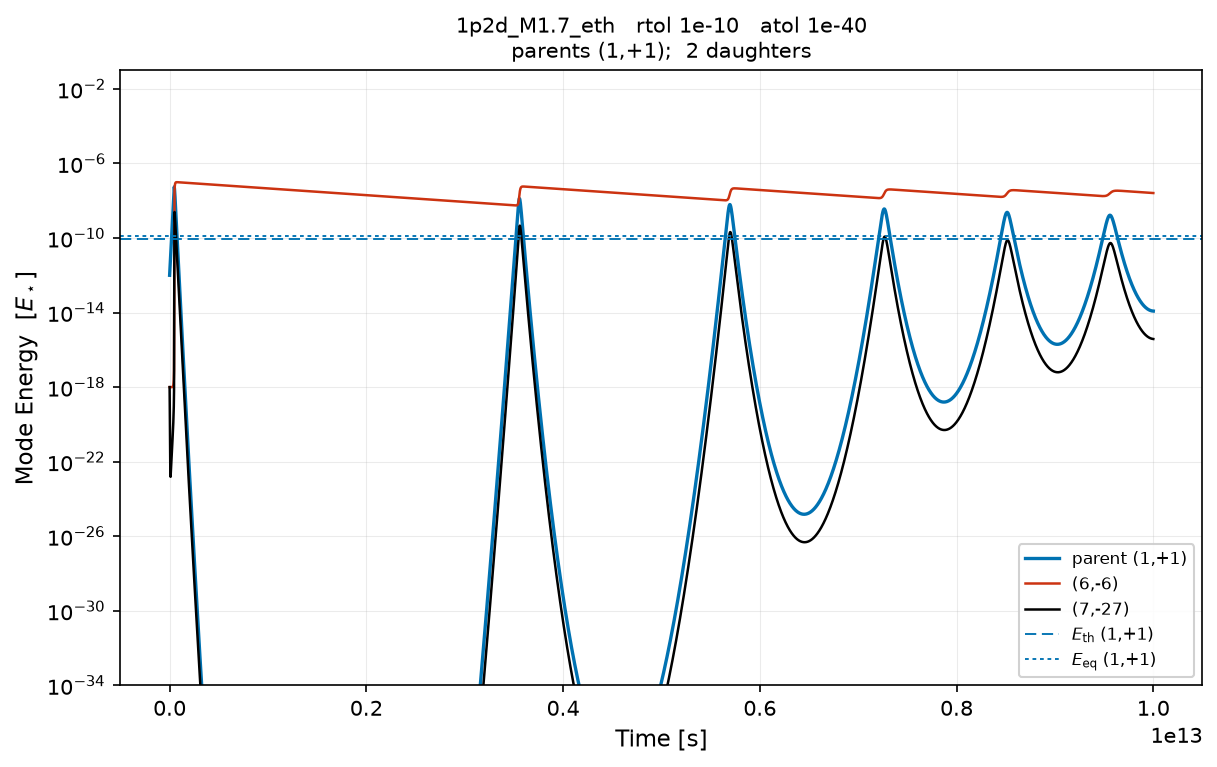
\includegraphics[width=0.21\textwidth,height=0.1323\textwidth]{../plots/rk8pd/1p2d_M1.7_eth/r1e-10_a1e-40.png} & {\fboxsep0pt\fbox{\parbox[b][\dimexpr0.1323\textwidth-2\fboxrule][c]{\dimexpr0.21\textwidth-2\fboxrule}{\centering\scriptsize not run}}} & {\fboxsep0pt\fbox{\parbox[b][\dimexpr0.1323\textwidth-2\fboxrule][c]{\dimexpr0.21\textwidth-2\fboxrule}{\centering\scriptsize not run}}} & 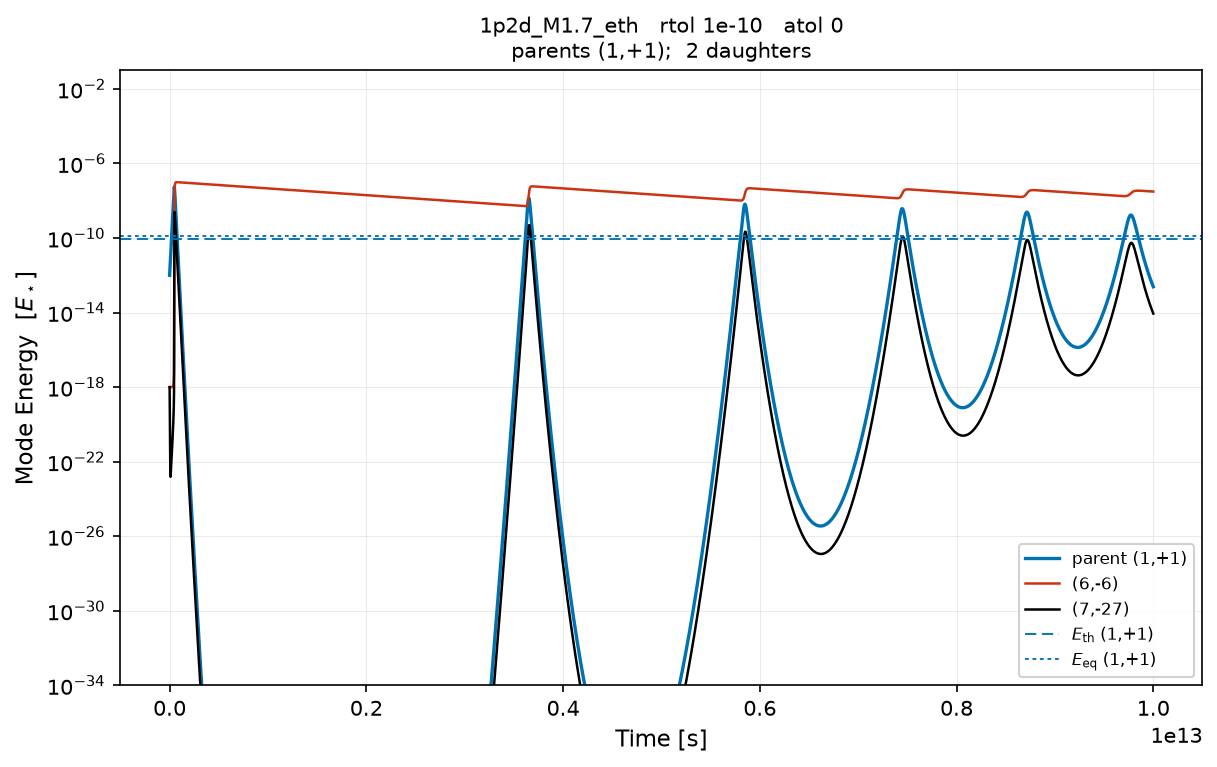
\includegraphics[width=0.21\textwidth,height=0.1323\textwidth]{../plots/rk8pd/1p2d_M1.7_eth/r1e-10_a0.png} \\[-1pt]
 & \parbox[t]{0.21\textwidth}{\centering\scriptsize 1.54\,M steps, 3.9\,s} & \parbox[t]{0.21\textwidth}{\centering\scriptsize --} & \parbox[t]{0.21\textwidth}{\centering\scriptsize --} & \parbox[t]{0.21\textwidth}{\centering\scriptsize 1.87\,M steps, 4.8\,s} \\[2pt]
\rotatebox{90}{\parbox{0.1323\textwidth}{\centering\scriptsize\bfseries rtol $10^{-12}$}} & 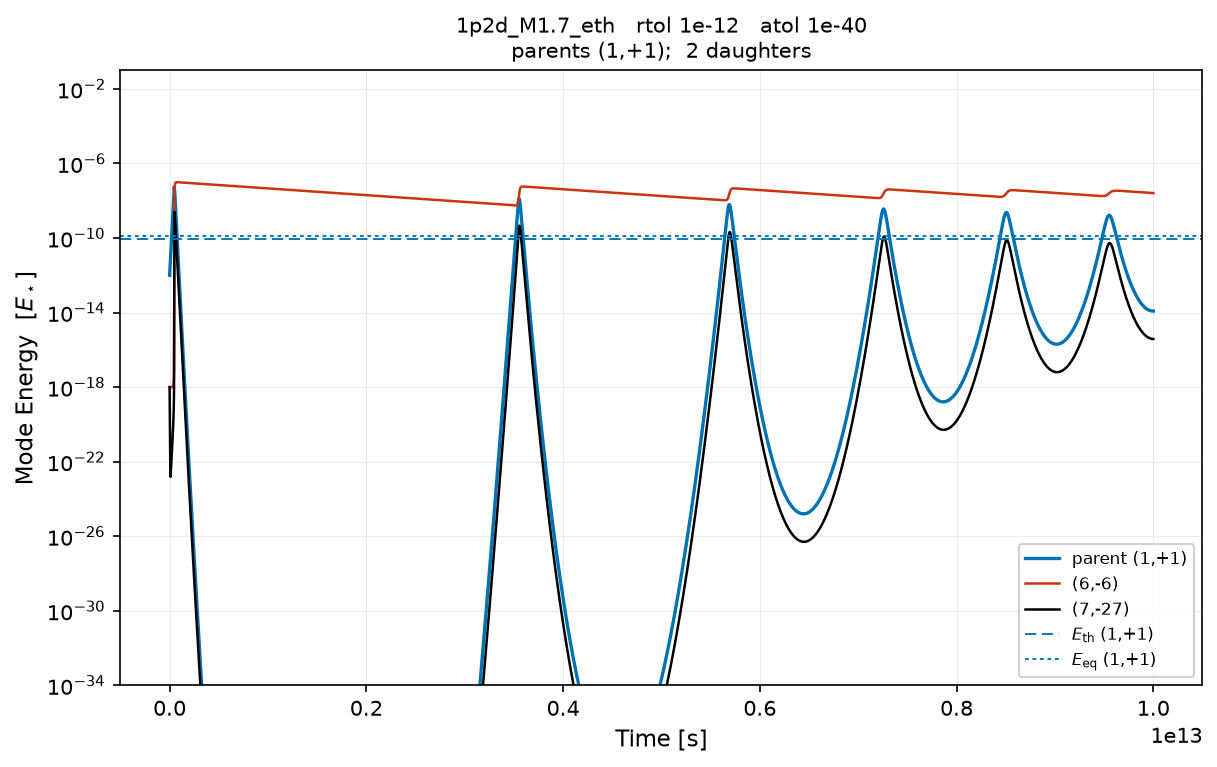
\includegraphics[width=0.21\textwidth,height=0.1323\textwidth]{../plots/rk8pd/1p2d_M1.7_eth/r1e-12_a1e-40.png} & 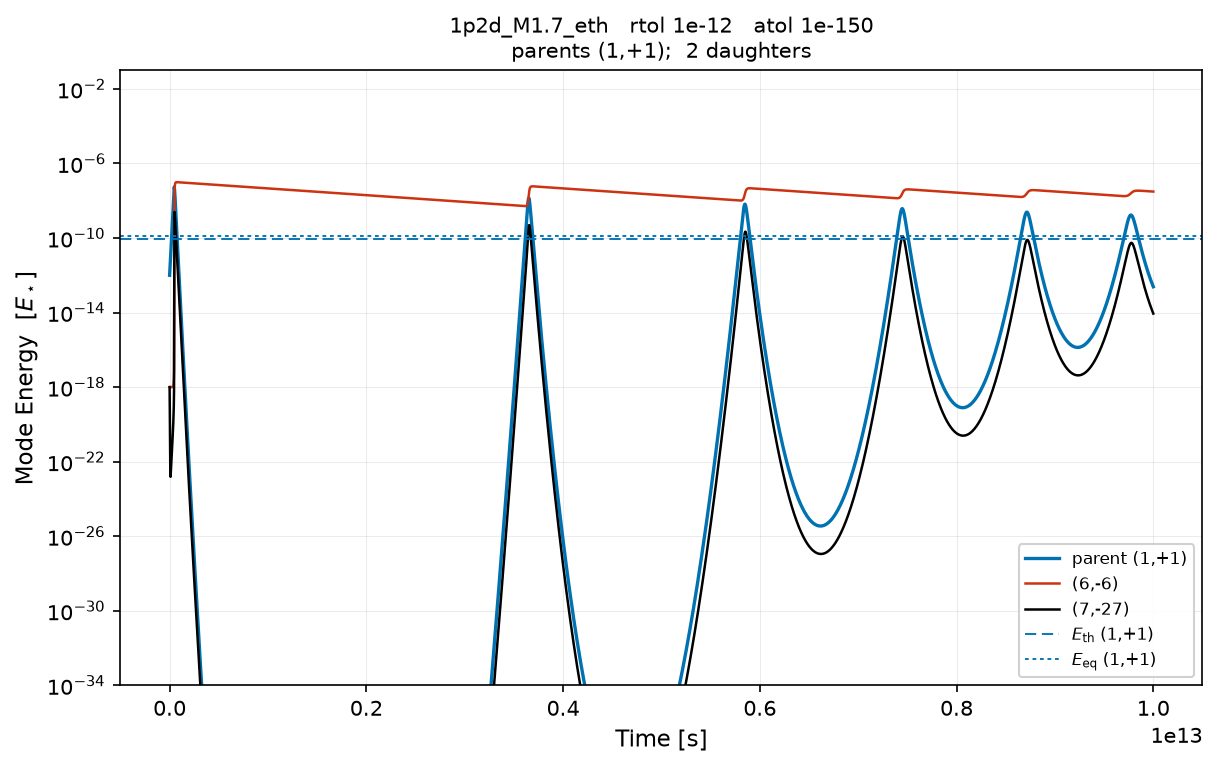
\includegraphics[width=0.21\textwidth,height=0.1323\textwidth]{../plots/rk8pd/1p2d_M1.7_eth/r1e-12_a1e-150.png} & 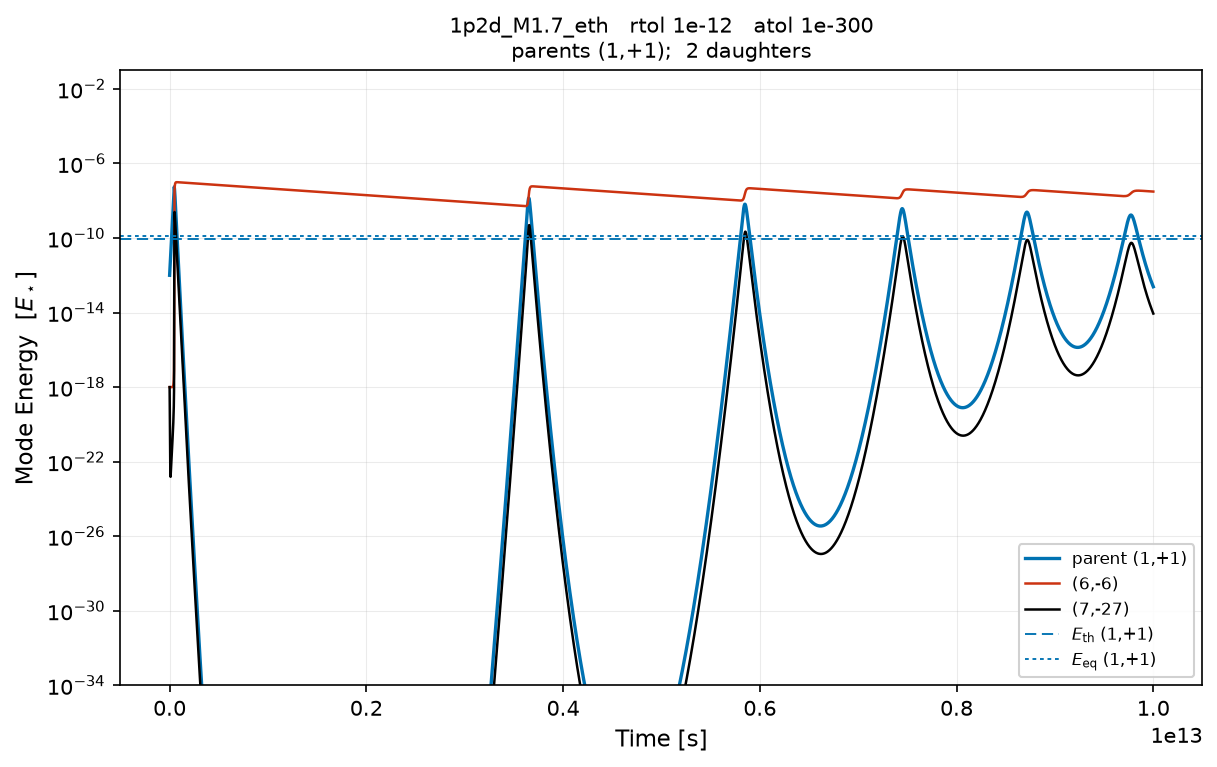
\includegraphics[width=0.21\textwidth,height=0.1323\textwidth]{../plots/rk8pd/1p2d_M1.7_eth/r1e-12_a1e-300.png} & 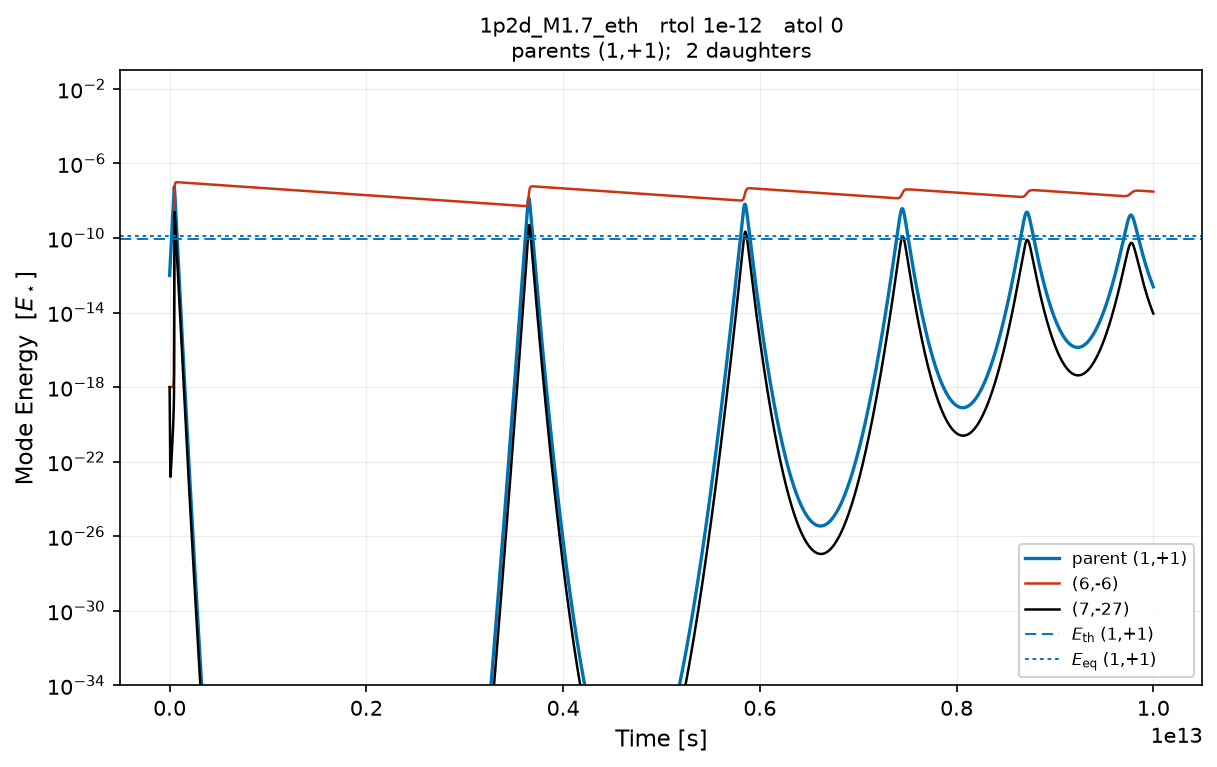
\includegraphics[width=0.21\textwidth,height=0.1323\textwidth]{../plots/rk8pd/1p2d_M1.7_eth/r1e-12_a0.png} \\[-1pt]
 & \parbox[t]{0.21\textwidth}{\centering\scriptsize 2.56\,M steps, 4.4\,s} & \parbox[t]{0.21\textwidth}{\centering\scriptsize 3.16\,M steps, 4.5\,s} & \parbox[t]{0.21\textwidth}{\centering\scriptsize 3.16\,M steps, 4.6\,s} & \parbox[t]{0.21\textwidth}{\centering\scriptsize 3.16\,M steps, 7.8\,s} \\[2pt]
\end{tabular}\par}
\par\noindent{\scriptsize\setlength\tabcolsep{3.5pt}\renewcommand\arraystretch{0.92}
\begin{tabular}{@{}llllrrrrrrr@{}}
\toprule
rtol & atol & stop & $t_{\rm stop}$ [s] & steps & rejected & RHS & Jac. & NL it. & lin. it. & wall [s] \\
\midrule
$10^{-8}$ & $10^{-40}$ & end & $1.00\times10^{13}$ & 953.2\,k & 101.3\,k & 12.39\,M & -- & -- & -- & 1.5 \\
 & $10^{-150}$ & end & $1.00\times10^{13}$ & 1.13\,M & 126.8\,k & 14.65\,M & -- & -- & -- & 2.3 \\
 & $10^{-300}$ & end & $1.00\times10^{13}$ & 1.13\,M & 126.8\,k & 14.65\,M & -- & -- & -- & 2.2 \\
 & $0$ & end & $1.00\times10^{13}$ & 1.13\,M & 126.8\,k & 14.65\,M & -- & -- & -- & 2.8 \\
\addlinespace[2pt]
$10^{-10}$ & $10^{-40}$ & end & $1.00\times10^{13}$ & 1.54\,M & 110.1\,k & 20.04\,M & -- & -- & -- & 3.9 \\
 & $10^{-150}$ & not run & \multicolumn{8}{l}{} \\
 & $10^{-300}$ & not run & \multicolumn{8}{l}{} \\
 & $0$ & end & $1.00\times10^{13}$ & 1.87\,M & 140.6\,k & 24.25\,M & -- & -- & -- & 4.8 \\
\addlinespace[2pt]
$10^{-12}$ & $10^{-40}$ & end & $1.00\times10^{13}$ & 2.56\,M & 116.1\,k & 33.27\,M & -- & -- & -- & 4.4 \\
 & $10^{-150}$ & end & $1.00\times10^{13}$ & 3.16\,M & 153.8\,k & 41.12\,M & -- & -- & -- & 4.5 \\
 & $10^{-300}$ & end & $1.00\times10^{13}$ & 3.16\,M & 153.8\,k & 41.12\,M & -- & -- & -- & 4.6 \\
 & $0$ & end & $1.00\times10^{13}$ & 3.16\,M & 153.8\,k & 41.12\,M & -- & -- & -- & 7.8 \\
\bottomrule
\end{tabular}}

\clearpage
\subsection{\texttt{1p2d\_M2.0T\_eth}: rk8pd, rtol $\times$ atol}
\noindent See \S\ref{net:1p2d_M2.0T_eth} for the network. 
\par\smallskip{\centering\begin{tabular}{@{}c@{\hspace{2pt}}c@{\hspace{2pt}}c@{\hspace{2pt}}c@{\hspace{2pt}}c@{}}
 & \small atol $10^{-40}$ & \small atol $10^{-150}$ & \small atol $10^{-300}$ & \small atol $0$ \\[1pt]
\rotatebox{90}{\parbox{0.1323\textwidth}{\centering\scriptsize\bfseries rtol $10^{-8}$}} & 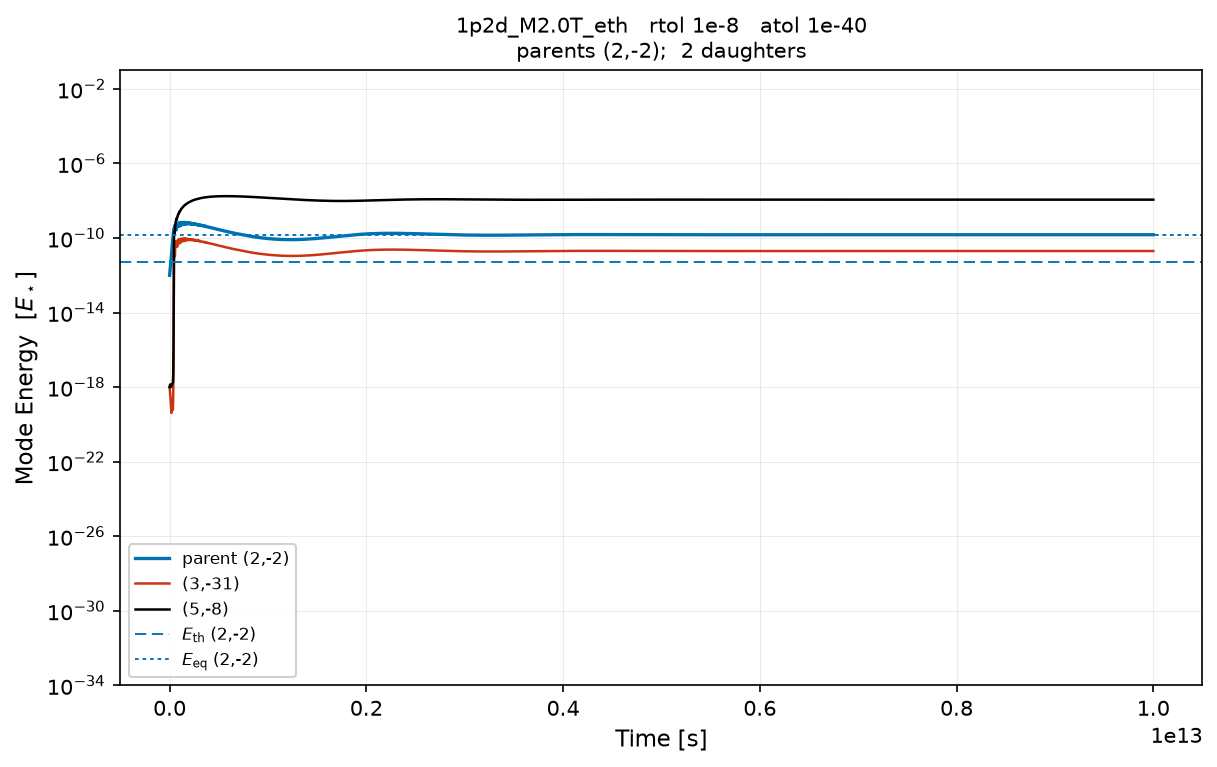
\includegraphics[width=0.21\textwidth,height=0.1323\textwidth]{../plots/rk8pd/1p2d_M2.0T_eth/r1e-8_a1e-40.png} & 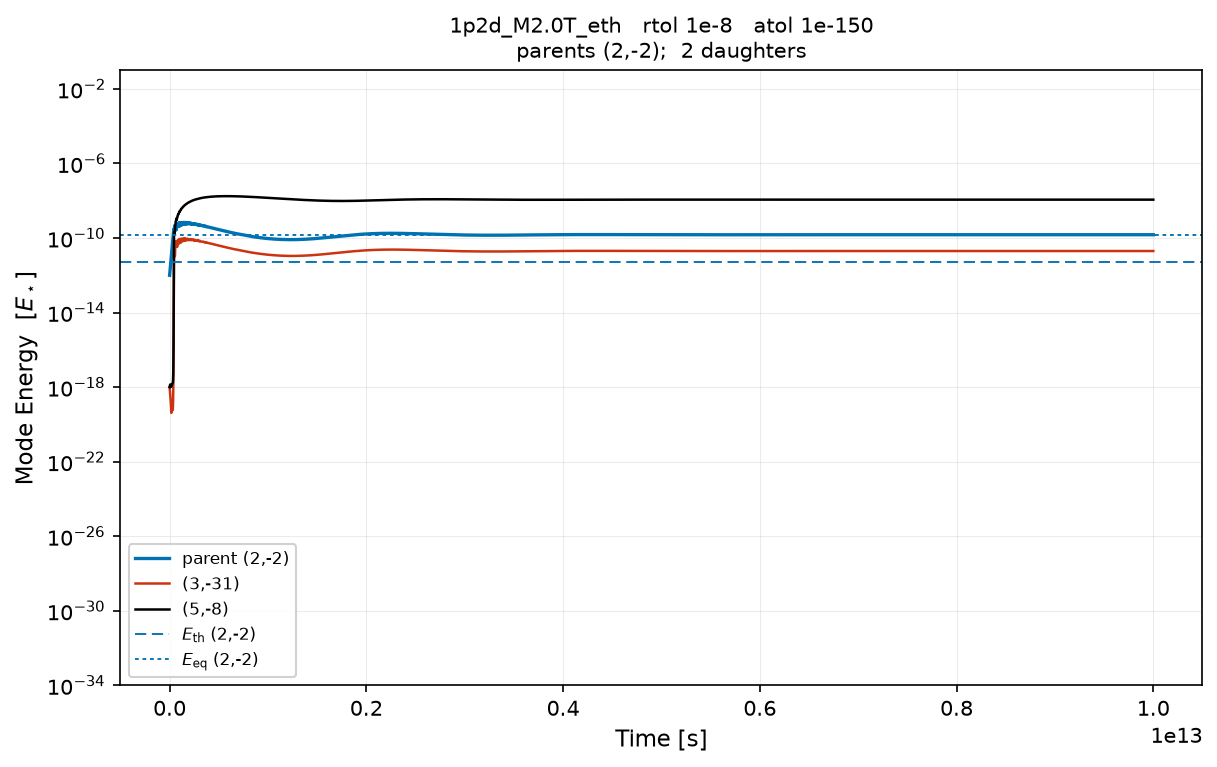
\includegraphics[width=0.21\textwidth,height=0.1323\textwidth]{../plots/rk8pd/1p2d_M2.0T_eth/r1e-8_a1e-150.png} & 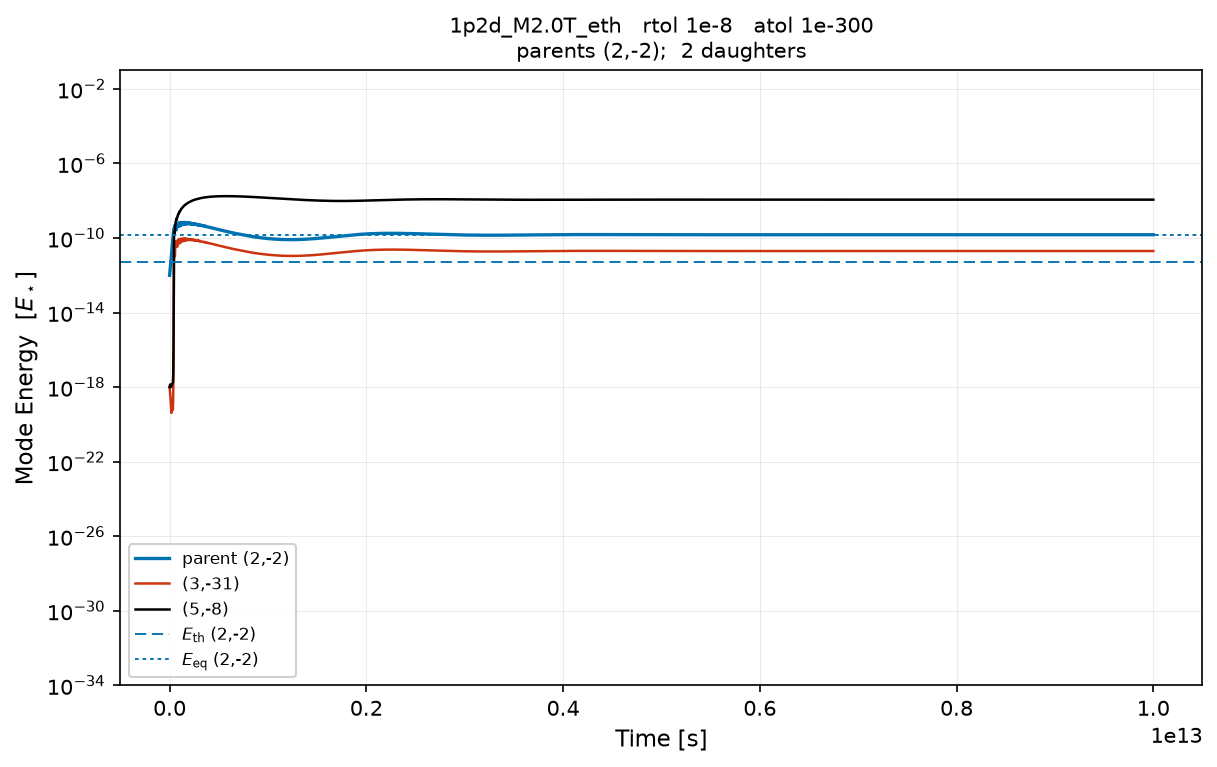
\includegraphics[width=0.21\textwidth,height=0.1323\textwidth]{../plots/rk8pd/1p2d_M2.0T_eth/r1e-8_a1e-300.png} & 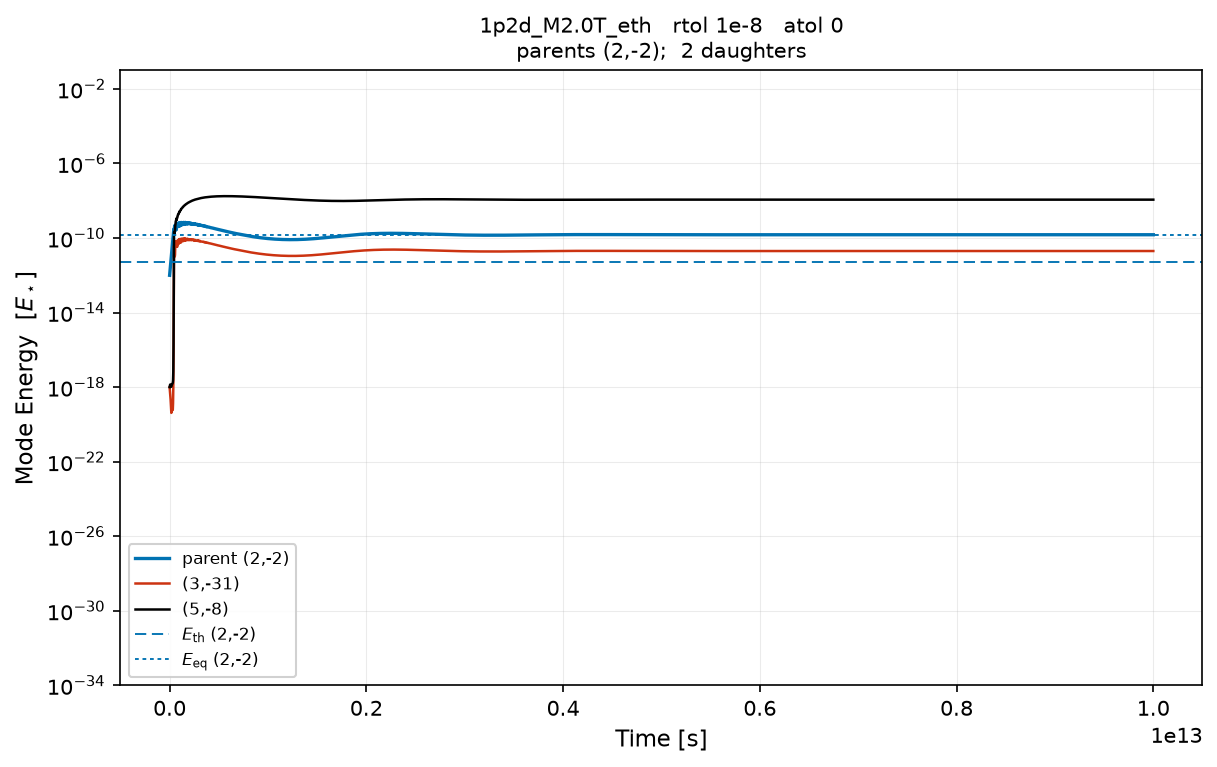
\includegraphics[width=0.21\textwidth,height=0.1323\textwidth]{../plots/rk8pd/1p2d_M2.0T_eth/r1e-8_a0.png} \\[-1pt]
 & \parbox[t]{0.21\textwidth}{\centering\scriptsize 385.4\,k steps, 0.4\,s} & \parbox[t]{0.21\textwidth}{\centering\scriptsize 385.4\,k steps, 0.6\,s} & \parbox[t]{0.21\textwidth}{\centering\scriptsize 385.4\,k steps, 0.8\,s} & \parbox[t]{0.21\textwidth}{\centering\scriptsize 385.4\,k steps, 0.9\,s} \\[2pt]
\rotatebox{90}{\parbox{0.1323\textwidth}{\centering\scriptsize\bfseries rtol $10^{-10}$}} & 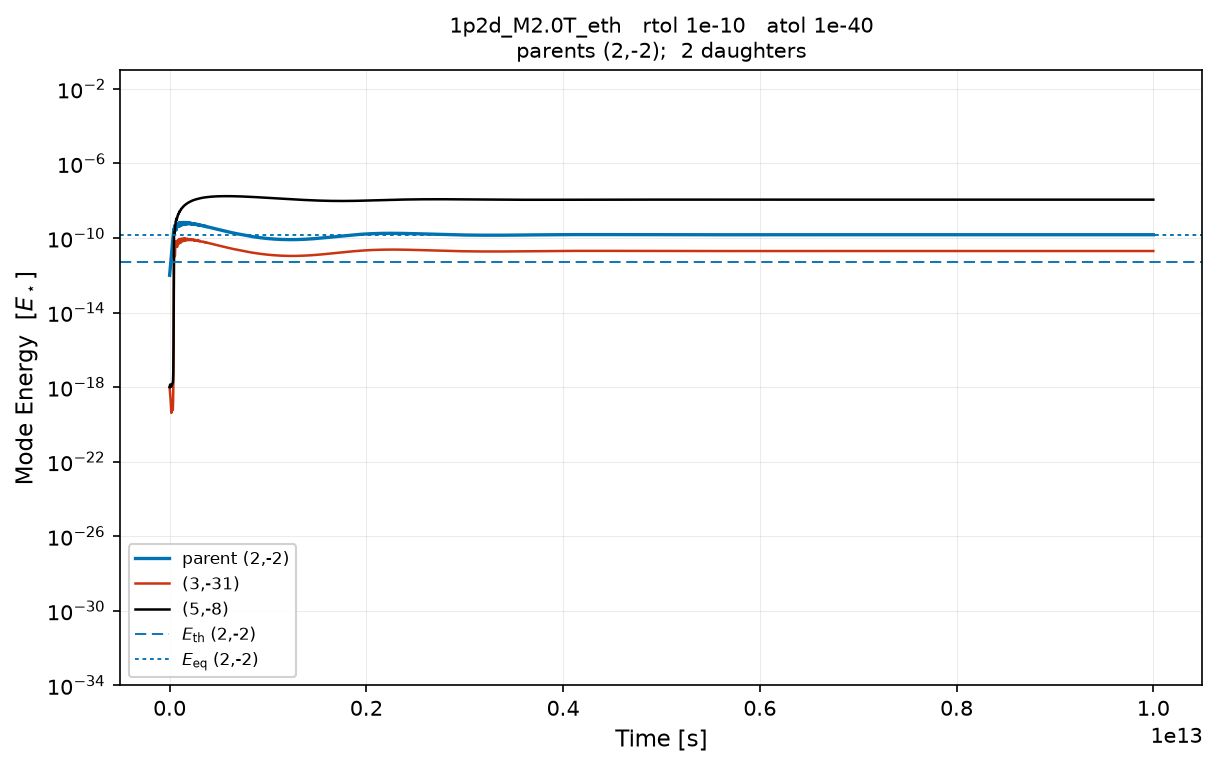
\includegraphics[width=0.21\textwidth,height=0.1323\textwidth]{../plots/rk8pd/1p2d_M2.0T_eth/r1e-10_a1e-40.png} & {\fboxsep0pt\fbox{\parbox[b][\dimexpr0.1323\textwidth-2\fboxrule][c]{\dimexpr0.21\textwidth-2\fboxrule}{\centering\scriptsize not run}}} & {\fboxsep0pt\fbox{\parbox[b][\dimexpr0.1323\textwidth-2\fboxrule][c]{\dimexpr0.21\textwidth-2\fboxrule}{\centering\scriptsize not run}}} & 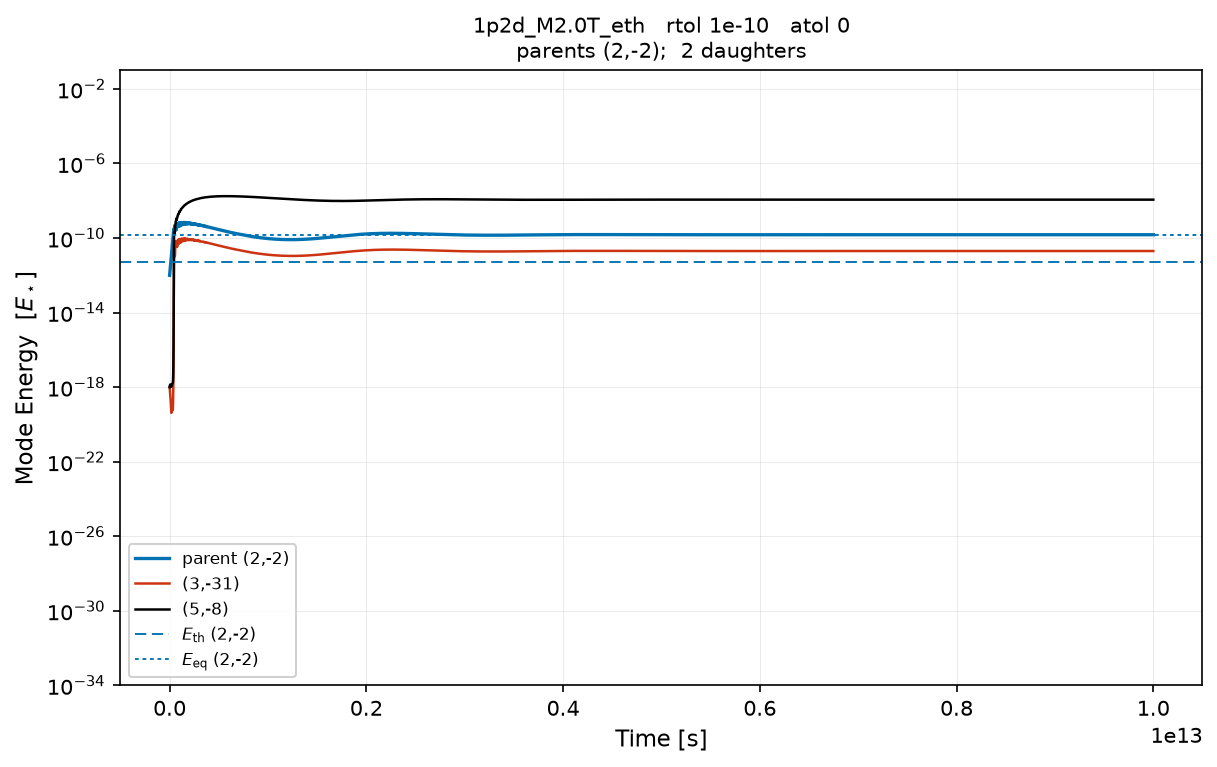
\includegraphics[width=0.21\textwidth,height=0.1323\textwidth]{../plots/rk8pd/1p2d_M2.0T_eth/r1e-10_a0.png} \\[-1pt]
 & \parbox[t]{0.21\textwidth}{\centering\scriptsize 604.0\,k steps, 0.8\,s} & \parbox[t]{0.21\textwidth}{\centering\scriptsize --} & \parbox[t]{0.21\textwidth}{\centering\scriptsize --} & \parbox[t]{0.21\textwidth}{\centering\scriptsize 604.0\,k steps, 0.9\,s} \\[2pt]
\rotatebox{90}{\parbox{0.1323\textwidth}{\centering\scriptsize\bfseries rtol $10^{-12}$}} & 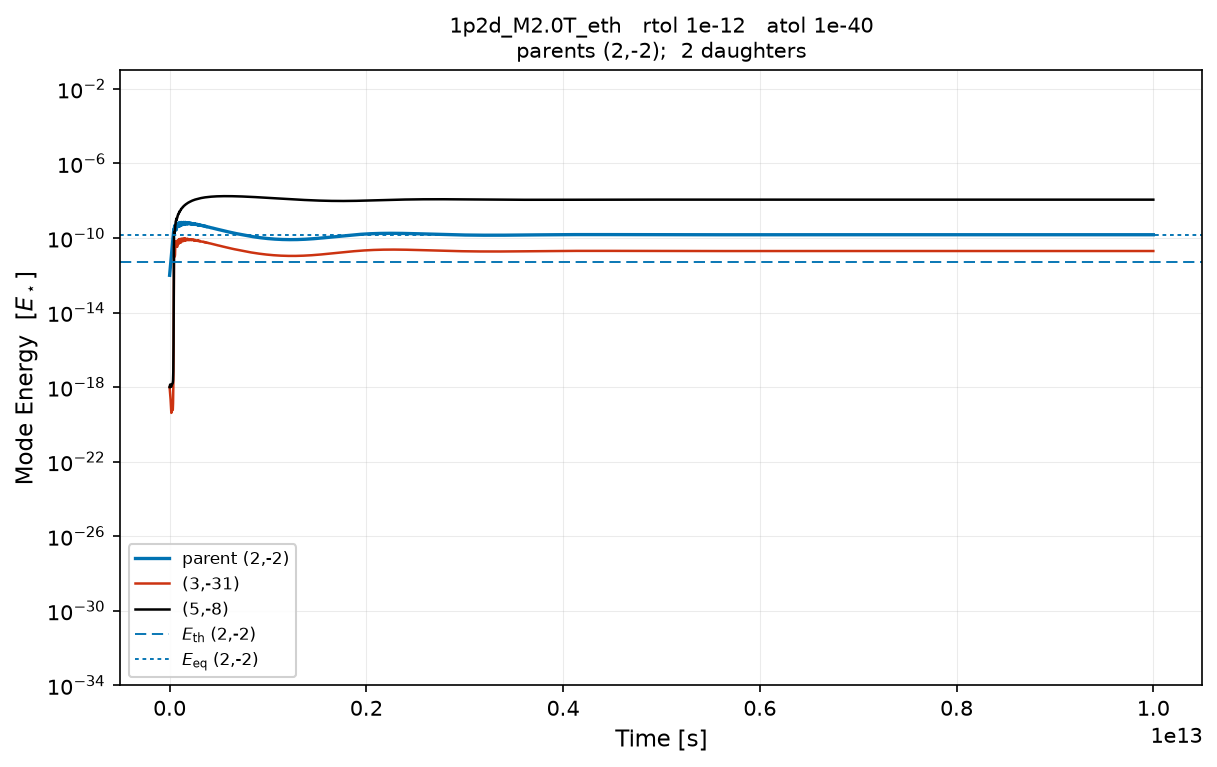
\includegraphics[width=0.21\textwidth,height=0.1323\textwidth]{../plots/rk8pd/1p2d_M2.0T_eth/r1e-12_a1e-40.png} & 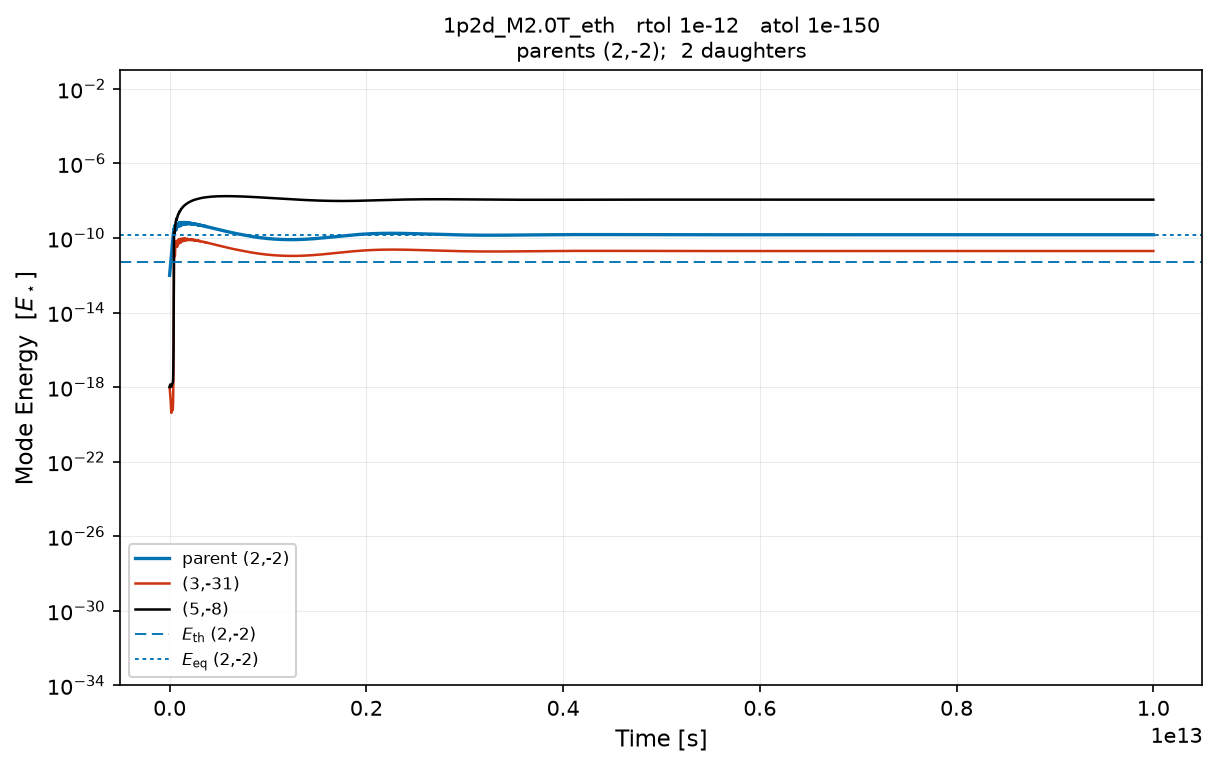
\includegraphics[width=0.21\textwidth,height=0.1323\textwidth]{../plots/rk8pd/1p2d_M2.0T_eth/r1e-12_a1e-150.png} & 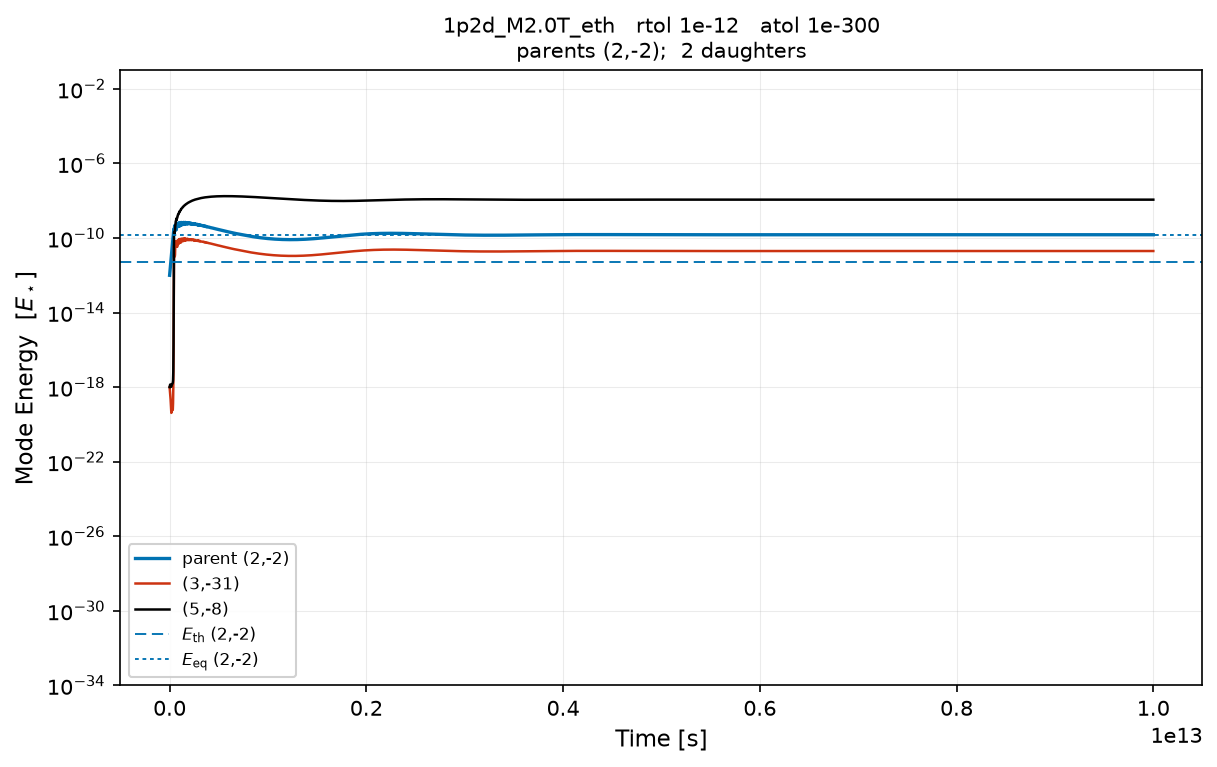
\includegraphics[width=0.21\textwidth,height=0.1323\textwidth]{../plots/rk8pd/1p2d_M2.0T_eth/r1e-12_a1e-300.png} & \includegraphics[width=0.21\textwidth,height=0.1323\textwidth]{../plots/rk8pd/1p2d_M2.0T_eth/r1e-12_a0.png} \\[-1pt]
 & \parbox[t]{0.21\textwidth}{\centering\scriptsize 1.03\,M steps, 2.5\,s} & \parbox[t]{0.21\textwidth}{\centering\scriptsize 1.03\,M steps, 1.6\,s} & \parbox[t]{0.21\textwidth}{\centering\scriptsize 1.03\,M steps, 1.5\,s} & \parbox[t]{0.21\textwidth}{\centering\scriptsize 1.03\,M steps, 1.8\,s} \\[2pt]
\end{tabular}\par}
\par\noindent{\scriptsize\setlength\tabcolsep{3.5pt}\renewcommand\arraystretch{0.92}
\begin{tabular}{@{}llllrrrrrrr@{}}
\toprule
rtol & atol & stop & $t_{\rm stop}$ [s] & steps & rejected & RHS & Jac. & NL it. & lin. it. & wall [s] \\
\midrule
$10^{-8}$ & $10^{-40}$ & end & $1.00\times10^{13}$ & 385.4\,k & 83.7\,k & 5.01\,M & -- & -- & -- & 0.4 \\
 & $10^{-150}$ & end & $1.00\times10^{13}$ & 385.4\,k & 83.7\,k & 5.01\,M & -- & -- & -- & 0.6 \\
 & $10^{-300}$ & end & $1.00\times10^{13}$ & 385.4\,k & 83.7\,k & 5.01\,M & -- & -- & -- & 0.8 \\
 & $0$ & end & $1.00\times10^{13}$ & 385.4\,k & 83.7\,k & 5.01\,M & -- & -- & -- & 0.9 \\
\addlinespace[2pt]
$10^{-10}$ & $10^{-40}$ & end & $1.00\times10^{13}$ & 604.0\,k & 87.8\,k & 7.85\,M & -- & -- & -- & 0.8 \\
 & $10^{-150}$ & not run & \multicolumn{8}{l}{} \\
 & $10^{-300}$ & not run & \multicolumn{8}{l}{} \\
 & $0$ & end & $1.00\times10^{13}$ & 604.0\,k & 87.8\,k & 7.85\,M & -- & -- & -- & 0.9 \\
\addlinespace[2pt]
$10^{-12}$ & $10^{-40}$ & end & $1.00\times10^{13}$ & 1.03\,M & 131.8\,k & 13.36\,M & -- & -- & -- & 2.5 \\
 & $10^{-150}$ & end & $1.00\times10^{13}$ & 1.03\,M & 131.8\,k & 13.36\,M & -- & -- & -- & 1.6 \\
 & $10^{-300}$ & end & $1.00\times10^{13}$ & 1.03\,M & 131.8\,k & 13.36\,M & -- & -- & -- & 1.5 \\
 & $0$ & end & $1.00\times10^{13}$ & 1.03\,M & 131.8\,k & 13.36\,M & -- & -- & -- & 1.8 \\
\bottomrule
\end{tabular}}

\clearpage
\subsection{\texttt{1p2d\_M2.0\_dgamma}: rk8pd, rtol $\times$ atol}
\noindent See \S\ref{net:1p2d_M2.0_dgamma} for the network. Deep dips between bursts.
\par\smallskip{\centering\begin{tabular}{@{}c@{\hspace{2pt}}c@{\hspace{2pt}}c@{\hspace{2pt}}c@{\hspace{2pt}}c@{}}
 & \small atol $10^{-40}$ & \small atol $10^{-150}$ & \small atol $10^{-300}$ & \small atol $0$ \\[1pt]
\rotatebox{90}{\parbox{0.1323\textwidth}{\centering\scriptsize\bfseries rtol $10^{-8}$}} & \includegraphics[width=0.21\textwidth,height=0.1323\textwidth]{../plots/rk8pd/1p2d_M2.0_dgamma/r1e-8_a1e-40.png} & \includegraphics[width=0.21\textwidth,height=0.1323\textwidth]{../plots/rk8pd/1p2d_M2.0_dgamma/r1e-8_a1e-150.png} & \includegraphics[width=0.21\textwidth,height=0.1323\textwidth]{../plots/rk8pd/1p2d_M2.0_dgamma/r1e-8_a1e-300.png} & \includegraphics[width=0.21\textwidth,height=0.1323\textwidth]{../plots/rk8pd/1p2d_M2.0_dgamma/r1e-8_a0.png} \\[-1pt]
 & \parbox[t]{0.21\textwidth}{\centering\scriptsize 6.61\,M steps, 9.5\,s} & \parbox[t]{0.21\textwidth}{\centering\scriptsize 8.24\,M steps, 15.6\,s} & \parbox[t]{0.21\textwidth}{\centering\scriptsize 9.26\,M steps, 13.5\,s} & \parbox[t]{0.21\textwidth}{\centering\scriptsize 9.26\,M steps, 20.4\,s} \\[2pt]
\rotatebox{90}{\parbox{0.1323\textwidth}{\centering\scriptsize\bfseries rtol $10^{-10}$}} & \includegraphics[width=0.21\textwidth,height=0.1323\textwidth]{../plots/rk8pd/1p2d_M2.0_dgamma/r1e-10_a1e-40.png} & {\fboxsep0pt\fbox{\parbox[b][\dimexpr0.1323\textwidth-2\fboxrule][c]{\dimexpr0.21\textwidth-2\fboxrule}{\centering\scriptsize not run}}} & {\fboxsep0pt\fbox{\parbox[b][\dimexpr0.1323\textwidth-2\fboxrule][c]{\dimexpr0.21\textwidth-2\fboxrule}{\centering\scriptsize not run}}} & \includegraphics[width=0.21\textwidth,height=0.1323\textwidth]{../plots/rk8pd/1p2d_M2.0_dgamma/r1e-10_a0.png} \\[-1pt]
 & \parbox[t]{0.21\textwidth}{\centering\scriptsize 10.60\,M steps, 19.0\,s} & \parbox[t]{0.21\textwidth}{\centering\scriptsize --} & \parbox[t]{0.21\textwidth}{\centering\scriptsize --} & \parbox[t]{0.21\textwidth}{\centering\scriptsize 15.47\,M steps, 35.0\,s} \\[2pt]
\rotatebox{90}{\parbox{0.1323\textwidth}{\centering\scriptsize\bfseries rtol $10^{-12}$}} & \includegraphics[width=0.21\textwidth,height=0.1323\textwidth]{../plots/rk8pd/1p2d_M2.0_dgamma/r1e-12_a1e-40.png} & \includegraphics[width=0.21\textwidth,height=0.1323\textwidth]{../plots/rk8pd/1p2d_M2.0_dgamma/r1e-12_a1e-150.png} & \includegraphics[width=0.21\textwidth,height=0.1323\textwidth]{../plots/rk8pd/1p2d_M2.0_dgamma/r1e-12_a1e-300.png} & \includegraphics[width=0.21\textwidth,height=0.1323\textwidth]{../plots/rk8pd/1p2d_M2.0_dgamma/r1e-12_a0.png} \\[-1pt]
 & \parbox[t]{0.21\textwidth}{\centering\scriptsize 17.32\,M steps, 34.3\,s} & \parbox[t]{0.21\textwidth}{\centering\scriptsize 22.42\,M steps, 33.3\,s} & \parbox[t]{0.21\textwidth}{\centering\scriptsize 26.08\,M steps, 32.1\,s} & \parbox[t]{0.21\textwidth}{\centering\scriptsize 26.08\,M steps, 50.2\,s} \\[2pt]
\end{tabular}\par}
\par\noindent{\scriptsize\setlength\tabcolsep{3.5pt}\renewcommand\arraystretch{0.92}
\begin{tabular}{@{}llllrrrrrrr@{}}
\toprule
rtol & atol & stop & $t_{\rm stop}$ [s] & steps & rejected & RHS & Jac. & NL it. & lin. it. & wall [s] \\
\midrule
$10^{-8}$ & $10^{-40}$ & end & $1.00\times10^{13}$ & 6.61\,M & 575.7\,k & 85.89\,M & -- & -- & -- & 9.5 \\
 & $10^{-150}$ & end & $1.00\times10^{13}$ & 8.24\,M & 937.9\,k & 107.11\,M & -- & -- & -- & 15.6 \\
 & $10^{-300}$ & end & $1.00\times10^{13}$ & 9.26\,M & 1.04\,M & 120.43\,M & -- & -- & -- & 13.5 \\
 & $0$ & end & $1.00\times10^{13}$ & 9.26\,M & 1.04\,M & 120.43\,M & -- & -- & -- & 20.4 \\
\addlinespace[2pt]
$10^{-10}$ & $10^{-40}$ & end & $1.00\times10^{13}$ & 10.60\,M & 653.6\,k & 137.86\,M & -- & -- & -- & 19.0 \\
 & $10^{-150}$ & not run & \multicolumn{8}{l}{} \\
 & $10^{-300}$ & not run & \multicolumn{8}{l}{} \\
 & $0$ & end & $1.00\times10^{13}$ & 15.47\,M & 1.23\,M & 201.05\,M & -- & -- & -- & 35.0 \\
\addlinespace[2pt]
$10^{-12}$ & $10^{-40}$ & end & $1.00\times10^{13}$ & 17.32\,M & 702.1\,k & 225.19\,M & -- & -- & -- & 34.3 \\
 & $10^{-150}$ & end & $1.00\times10^{13}$ & 22.42\,M & 1.16\,M & 291.47\,M & -- & -- & -- & 33.3 \\
 & $10^{-300}$ & end & $1.00\times10^{13}$ & 26.08\,M & 1.34\,M & 339.08\,M & -- & -- & -- & 32.1 \\
 & $0$ & end & $1.00\times10^{13}$ & 26.08\,M & 1.34\,M & 339.08\,M & -- & -- & -- & 50.2 \\
\bottomrule
\end{tabular}}

\clearpage
\subsection{\texttt{1p4d\_M1.7\_eth}: rk8pd, rtol $\times$ atol}
\noindent See \S\ref{net:1p4d_M1.7_eth} for the network. Runaway near $3\times10^{11}$\,s.
\par\smallskip{\centering\begin{tabular}{@{}c@{\hspace{2pt}}c@{\hspace{2pt}}c@{\hspace{2pt}}c@{\hspace{2pt}}c@{}}
 & \small atol $10^{-40}$ & \small atol $10^{-150}$ & \small atol $10^{-300}$ & \small atol $0$ \\[1pt]
\rotatebox{90}{\parbox{0.1323\textwidth}{\centering\scriptsize\bfseries rtol $10^{-8}$}} & \includegraphics[width=0.21\textwidth,height=0.1323\textwidth]{../plots/rk8pd/1p4d_M1.7_eth/r1e-8_a1e-40.png} & \includegraphics[width=0.21\textwidth,height=0.1323\textwidth]{../plots/rk8pd/1p4d_M1.7_eth/r1e-8_a1e-150.png} & \includegraphics[width=0.21\textwidth,height=0.1323\textwidth]{../plots/rk8pd/1p4d_M1.7_eth/r1e-8_a1e-300.png} & \includegraphics[width=0.21\textwidth,height=0.1323\textwidth]{../plots/rk8pd/1p4d_M1.7_eth/r1e-8_a0.png} \\[-1pt]
 & \parbox[t]{0.21\textwidth}{\centering\scriptsize 7.58\,M steps, 19.8\,s, runaway} & \parbox[t]{0.21\textwidth}{\centering\scriptsize 7.58\,M steps, 17.7\,s, runaway} & \parbox[t]{0.21\textwidth}{\centering\scriptsize 7.58\,M steps, 18.4\,s, runaway} & \parbox[t]{0.21\textwidth}{\centering\scriptsize 7.58\,M steps, 19.8\,s, runaway} \\[2pt]
\rotatebox{90}{\parbox{0.1323\textwidth}{\centering\scriptsize\bfseries rtol $10^{-10}$}} & \includegraphics[width=0.21\textwidth,height=0.1323\textwidth]{../plots/rk8pd/1p4d_M1.7_eth/r1e-10_a1e-40.png} & {\fboxsep0pt\fbox{\parbox[b][\dimexpr0.1323\textwidth-2\fboxrule][c]{\dimexpr0.21\textwidth-2\fboxrule}{\centering\scriptsize not run}}} & {\fboxsep0pt\fbox{\parbox[b][\dimexpr0.1323\textwidth-2\fboxrule][c]{\dimexpr0.21\textwidth-2\fboxrule}{\centering\scriptsize not run}}} & \includegraphics[width=0.21\textwidth,height=0.1323\textwidth]{../plots/rk8pd/1p4d_M1.7_eth/r1e-10_a0.png} \\[-1pt]
 & \parbox[t]{0.21\textwidth}{\centering\scriptsize 13.64\,M steps, 41.1\,s, runaway} & \parbox[t]{0.21\textwidth}{\centering\scriptsize --} & \parbox[t]{0.21\textwidth}{\centering\scriptsize --} & \parbox[t]{0.21\textwidth}{\centering\scriptsize 13.64\,M steps, 36.1\,s, runaway} \\[2pt]
\rotatebox{90}{\parbox{0.1323\textwidth}{\centering\scriptsize\bfseries rtol $10^{-12}$}} & \includegraphics[width=0.21\textwidth,height=0.1323\textwidth]{../plots/rk8pd/1p4d_M1.7_eth/r1e-12_a1e-40.png} & \includegraphics[width=0.21\textwidth,height=0.1323\textwidth]{../plots/rk8pd/1p4d_M1.7_eth/r1e-12_a1e-150.png} & \includegraphics[width=0.21\textwidth,height=0.1323\textwidth]{../plots/rk8pd/1p4d_M1.7_eth/r1e-12_a1e-300.png} & \includegraphics[width=0.21\textwidth,height=0.1323\textwidth]{../plots/rk8pd/1p4d_M1.7_eth/r1e-12_a0.png} \\[-1pt]
 & \parbox[t]{0.21\textwidth}{\centering\scriptsize 22.63\,M steps, 58.6\,s, runaway} & \parbox[t]{0.21\textwidth}{\centering\scriptsize 22.63\,M steps, 57.4\,s, runaway} & \parbox[t]{0.21\textwidth}{\centering\scriptsize 22.63\,M steps, 57.3\,s, runaway} & \parbox[t]{0.21\textwidth}{\centering\scriptsize 22.63\,M steps, 82.7\,s, runaway} \\[2pt]
\end{tabular}\par}
\par\noindent{\scriptsize\setlength\tabcolsep{3.5pt}\renewcommand\arraystretch{0.92}
\begin{tabular}{@{}llllrrrrrrr@{}}
\toprule
rtol & atol & stop & $t_{\rm stop}$ [s] & steps & rejected & RHS & Jac. & NL it. & lin. it. & wall [s] \\
\midrule
$10^{-8}$ & $10^{-40}$ & runaway & $3.01\times10^{11}$ & 7.58\,M & 1.01\,M & 98.48\,M & -- & -- & -- & 19.8 \\
 & $10^{-150}$ & runaway & $3.01\times10^{11}$ & 7.58\,M & 1.01\,M & 98.48\,M & -- & -- & -- & 17.7 \\
 & $10^{-300}$ & runaway & $3.01\times10^{11}$ & 7.58\,M & 1.01\,M & 98.48\,M & -- & -- & -- & 18.4 \\
 & $0$ & runaway & $3.01\times10^{11}$ & 7.58\,M & 1.01\,M & 98.48\,M & -- & -- & -- & 19.8 \\
\addlinespace[2pt]
$10^{-10}$ & $10^{-40}$ & runaway & $3.01\times10^{11}$ & 13.64\,M & 1.93\,M & 177.26\,M & -- & -- & -- & 41.1 \\
 & $10^{-150}$ & not run & \multicolumn{8}{l}{} \\
 & $10^{-300}$ & not run & \multicolumn{8}{l}{} \\
 & $0$ & runaway & $3.01\times10^{11}$ & 13.64\,M & 1.93\,M & 177.29\,M & -- & -- & -- & 36.1 \\
\addlinespace[2pt]
$10^{-12}$ & $10^{-40}$ & runaway & $3.01\times10^{11}$ & 22.63\,M & 2.32\,M & 294.20\,M & -- & -- & -- & 58.6 \\
 & $10^{-150}$ & runaway & $3.01\times10^{11}$ & 22.63\,M & 2.33\,M & 294.20\,M & -- & -- & -- & 57.4 \\
 & $10^{-300}$ & runaway & $3.01\times10^{11}$ & 22.63\,M & 2.33\,M & 294.20\,M & -- & -- & -- & 57.3 \\
 & $0$ & runaway & $3.01\times10^{11}$ & 22.63\,M & 2.33\,M & 294.20\,M & -- & -- & -- & 82.7 \\
\bottomrule
\end{tabular}}

\clearpage
\subsection{\texttt{1p4d\_M2.0T\_eth}: rk8pd, rtol $\times$ atol}
\noindent See \S\ref{net:1p4d_M2.0T_eth} for the network. 
\par\smallskip{\centering\begin{tabular}{@{}c@{\hspace{2pt}}c@{\hspace{2pt}}c@{\hspace{2pt}}c@{\hspace{2pt}}c@{}}
 & \small atol $10^{-40}$ & \small atol $10^{-150}$ & \small atol $10^{-300}$ & \small atol $0$ \\[1pt]
\rotatebox{90}{\parbox{0.1323\textwidth}{\centering\scriptsize\bfseries rtol $10^{-8}$}} & \includegraphics[width=0.21\textwidth,height=0.1323\textwidth]{../plots/rk8pd/1p4d_M2.0T_eth/r1e-8_a1e-40.png} & \includegraphics[width=0.21\textwidth,height=0.1323\textwidth]{../plots/rk8pd/1p4d_M2.0T_eth/r1e-8_a1e-150.png} & \includegraphics[width=0.21\textwidth,height=0.1323\textwidth]{../plots/rk8pd/1p4d_M2.0T_eth/r1e-8_a1e-300.png} & \includegraphics[width=0.21\textwidth,height=0.1323\textwidth]{../plots/rk8pd/1p4d_M2.0T_eth/r1e-8_a0.png} \\[-1pt]
 & \parbox[t]{0.21\textwidth}{\centering\scriptsize 618.4\,k steps, 1.8\,s} & \parbox[t]{0.21\textwidth}{\centering\scriptsize 618.5\,k steps, 2.5\,s} & \parbox[t]{0.21\textwidth}{\centering\scriptsize 618.5\,k steps, 1.2\,s} & \parbox[t]{0.21\textwidth}{\centering\scriptsize 618.5\,k steps, 2.7\,s} \\[2pt]
\rotatebox{90}{\parbox{0.1323\textwidth}{\centering\scriptsize\bfseries rtol $10^{-10}$}} & \includegraphics[width=0.21\textwidth,height=0.1323\textwidth]{../plots/rk8pd/1p4d_M2.0T_eth/r1e-10_a1e-40.png} & {\fboxsep0pt\fbox{\parbox[b][\dimexpr0.1323\textwidth-2\fboxrule][c]{\dimexpr0.21\textwidth-2\fboxrule}{\centering\scriptsize not run}}} & {\fboxsep0pt\fbox{\parbox[b][\dimexpr0.1323\textwidth-2\fboxrule][c]{\dimexpr0.21\textwidth-2\fboxrule}{\centering\scriptsize not run}}} & \includegraphics[width=0.21\textwidth,height=0.1323\textwidth]{../plots/rk8pd/1p4d_M2.0T_eth/r1e-10_a0.png} \\[-1pt]
 & \parbox[t]{0.21\textwidth}{\centering\scriptsize 1.47\,M steps, 4.5\,s} & \parbox[t]{0.21\textwidth}{\centering\scriptsize --} & \parbox[t]{0.21\textwidth}{\centering\scriptsize --} & \parbox[t]{0.21\textwidth}{\centering\scriptsize 1.47\,M steps, 4.6\,s} \\[2pt]
\rotatebox{90}{\parbox{0.1323\textwidth}{\centering\scriptsize\bfseries rtol $10^{-12}$}} & \includegraphics[width=0.21\textwidth,height=0.1323\textwidth]{../plots/rk8pd/1p4d_M2.0T_eth/r1e-12_a1e-40.png} & \includegraphics[width=0.21\textwidth,height=0.1323\textwidth]{../plots/rk8pd/1p4d_M2.0T_eth/r1e-12_a1e-150.png} & \includegraphics[width=0.21\textwidth,height=0.1323\textwidth]{../plots/rk8pd/1p4d_M2.0T_eth/r1e-12_a1e-300.png} & \includegraphics[width=0.21\textwidth,height=0.1323\textwidth]{../plots/rk8pd/1p4d_M2.0T_eth/r1e-12_a0.png} \\[-1pt]
 & \parbox[t]{0.21\textwidth}{\centering\scriptsize 2.37\,M steps, 9.4\,s} & \parbox[t]{0.21\textwidth}{\centering\scriptsize 2.37\,M steps, 6.6\,s} & \parbox[t]{0.21\textwidth}{\centering\scriptsize 2.37\,M steps, 4.8\,s} & \parbox[t]{0.21\textwidth}{\centering\scriptsize 2.37\,M steps, 9.2\,s} \\[2pt]
\end{tabular}\par}
\par\noindent{\scriptsize\setlength\tabcolsep{3.5pt}\renewcommand\arraystretch{0.92}
\begin{tabular}{@{}llllrrrrrrr@{}}
\toprule
rtol & atol & stop & $t_{\rm stop}$ [s] & steps & rejected & RHS & Jac. & NL it. & lin. it. & wall [s] \\
\midrule
$10^{-8}$ & $10^{-40}$ & end & $1.00\times10^{13}$ & 618.4\,k & 18.4\,k & 8.04\,M & -- & -- & -- & 1.8 \\
 & $10^{-150}$ & end & $1.00\times10^{13}$ & 618.5\,k & 18.4\,k & 8.04\,M & -- & -- & -- & 2.5 \\
 & $10^{-300}$ & end & $1.00\times10^{13}$ & 618.5\,k & 18.4\,k & 8.04\,M & -- & -- & -- & 1.2 \\
 & $0$ & end & $1.00\times10^{13}$ & 618.5\,k & 18.4\,k & 8.04\,M & -- & -- & -- & 2.7 \\
\addlinespace[2pt]
$10^{-10}$ & $10^{-40}$ & end & $1.00\times10^{13}$ & 1.47\,M & 287.4\,k & 19.11\,M & -- & -- & -- & 4.5 \\
 & $10^{-150}$ & not run & \multicolumn{8}{l}{} \\
 & $10^{-300}$ & not run & \multicolumn{8}{l}{} \\
 & $0$ & end & $1.00\times10^{13}$ & 1.47\,M & 287.3\,k & 19.11\,M & -- & -- & -- & 4.6 \\
\addlinespace[2pt]
$10^{-12}$ & $10^{-40}$ & end & $1.00\times10^{13}$ & 2.37\,M & 303.5\,k & 30.87\,M & -- & -- & -- & 9.4 \\
 & $10^{-150}$ & end & $1.00\times10^{13}$ & 2.37\,M & 303.3\,k & 30.87\,M & -- & -- & -- & 6.6 \\
 & $10^{-300}$ & end & $1.00\times10^{13}$ & 2.37\,M & 303.3\,k & 30.87\,M & -- & -- & -- & 4.8 \\
 & $0$ & end & $1.00\times10^{13}$ & 2.37\,M & 303.3\,k & 30.87\,M & -- & -- & -- & 9.2 \\
\bottomrule
\end{tabular}}

\clearpage
\subsection{\texttt{1p4d\_M2.0\_eth}: rk8pd, rtol $\times$ atol}
\noindent See \S\ref{net:1p4d_M2.0_eth} for the network. 
\par\smallskip{\centering\begin{tabular}{@{}c@{\hspace{2pt}}c@{\hspace{2pt}}c@{\hspace{2pt}}c@{\hspace{2pt}}c@{}}
 & \small atol $10^{-40}$ & \small atol $10^{-150}$ & \small atol $10^{-300}$ & \small atol $0$ \\[1pt]
\rotatebox{90}{\parbox{0.1323\textwidth}{\centering\scriptsize\bfseries rtol $10^{-8}$}} & \includegraphics[width=0.21\textwidth,height=0.1323\textwidth]{../plots/rk8pd/1p4d_M2.0_eth/r1e-8_a1e-40.png} & \includegraphics[width=0.21\textwidth,height=0.1323\textwidth]{../plots/rk8pd/1p4d_M2.0_eth/r1e-8_a1e-150.png} & \includegraphics[width=0.21\textwidth,height=0.1323\textwidth]{../plots/rk8pd/1p4d_M2.0_eth/r1e-8_a1e-300.png} & \includegraphics[width=0.21\textwidth,height=0.1323\textwidth]{../plots/rk8pd/1p4d_M2.0_eth/r1e-8_a0.png} \\[-1pt]
 & \parbox[t]{0.21\textwidth}{\centering\scriptsize 2.41\,M steps, 5.2\,s} & \parbox[t]{0.21\textwidth}{\centering\scriptsize 2.41\,M steps, 10.5\,s} & \parbox[t]{0.21\textwidth}{\centering\scriptsize 2.41\,M steps, 7.6\,s} & \parbox[t]{0.21\textwidth}{\centering\scriptsize 2.41\,M steps, 10.1\,s} \\[2pt]
\rotatebox{90}{\parbox{0.1323\textwidth}{\centering\scriptsize\bfseries rtol $10^{-10}$}} & \includegraphics[width=0.21\textwidth,height=0.1323\textwidth]{../plots/rk8pd/1p4d_M2.0_eth/r1e-10_a1e-40.png} & {\fboxsep0pt\fbox{\parbox[b][\dimexpr0.1323\textwidth-2\fboxrule][c]{\dimexpr0.21\textwidth-2\fboxrule}{\centering\scriptsize not run}}} & {\fboxsep0pt\fbox{\parbox[b][\dimexpr0.1323\textwidth-2\fboxrule][c]{\dimexpr0.21\textwidth-2\fboxrule}{\centering\scriptsize not run}}} & \includegraphics[width=0.21\textwidth,height=0.1323\textwidth]{../plots/rk8pd/1p4d_M2.0_eth/r1e-10_a0.png} \\[-1pt]
 & \parbox[t]{0.21\textwidth}{\centering\scriptsize 3.70\,M steps, 14.2\,s} & \parbox[t]{0.21\textwidth}{\centering\scriptsize --} & \parbox[t]{0.21\textwidth}{\centering\scriptsize --} & \parbox[t]{0.21\textwidth}{\centering\scriptsize 3.70\,M steps, 14.5\,s} \\[2pt]
\rotatebox{90}{\parbox{0.1323\textwidth}{\centering\scriptsize\bfseries rtol $10^{-12}$}} & \includegraphics[width=0.21\textwidth,height=0.1323\textwidth]{../plots/rk8pd/1p4d_M2.0_eth/r1e-12_a1e-40.png} & \includegraphics[width=0.21\textwidth,height=0.1323\textwidth]{../plots/rk8pd/1p4d_M2.0_eth/r1e-12_a1e-150.png} & \includegraphics[width=0.21\textwidth,height=0.1323\textwidth]{../plots/rk8pd/1p4d_M2.0_eth/r1e-12_a1e-300.png} & \includegraphics[width=0.21\textwidth,height=0.1323\textwidth]{../plots/rk8pd/1p4d_M2.0_eth/r1e-12_a0.png} \\[-1pt]
 & \parbox[t]{0.21\textwidth}{\centering\scriptsize 6.39\,M steps, 18.1\,s} & \parbox[t]{0.21\textwidth}{\centering\scriptsize 6.39\,M steps, 15.7\,s} & \parbox[t]{0.21\textwidth}{\centering\scriptsize 6.39\,M steps, 13.3\,s} & \parbox[t]{0.21\textwidth}{\centering\scriptsize 6.39\,M steps, 27.4\,s} \\[2pt]
\end{tabular}\par}
\par\noindent{\scriptsize\setlength\tabcolsep{3.5pt}\renewcommand\arraystretch{0.92}
\begin{tabular}{@{}llllrrrrrrr@{}}
\toprule
rtol & atol & stop & $t_{\rm stop}$ [s] & steps & rejected & RHS & Jac. & NL it. & lin. it. & wall [s] \\
\midrule
$10^{-8}$ & $10^{-40}$ & end & $1.00\times10^{13}$ & 2.41\,M & 469.8\,k & 31.29\,M & -- & -- & -- & 5.2 \\
 & $10^{-150}$ & end & $1.00\times10^{13}$ & 2.41\,M & 469.8\,k & 31.29\,M & -- & -- & -- & 10.5 \\
 & $10^{-300}$ & end & $1.00\times10^{13}$ & 2.41\,M & 469.8\,k & 31.29\,M & -- & -- & -- & 7.6 \\
 & $0$ & end & $1.00\times10^{13}$ & 2.41\,M & 469.8\,k & 31.29\,M & -- & -- & -- & 10.1 \\
\addlinespace[2pt]
$10^{-10}$ & $10^{-40}$ & end & $1.00\times10^{13}$ & 3.70\,M & 439.1\,k & 48.05\,M & -- & -- & -- & 14.2 \\
 & $10^{-150}$ & not run & \multicolumn{8}{l}{} \\
 & $10^{-300}$ & not run & \multicolumn{8}{l}{} \\
 & $0$ & end & $1.00\times10^{13}$ & 3.70\,M & 439.1\,k & 48.05\,M & -- & -- & -- & 14.5 \\
\addlinespace[2pt]
$10^{-12}$ & $10^{-40}$ & end & $1.00\times10^{13}$ & 6.39\,M & 647.9\,k & 83.13\,M & -- & -- & -- & 18.1 \\
 & $10^{-150}$ & end & $1.00\times10^{13}$ & 6.39\,M & 647.7\,k & 83.13\,M & -- & -- & -- & 15.7 \\
 & $10^{-300}$ & end & $1.00\times10^{13}$ & 6.39\,M & 647.7\,k & 83.13\,M & -- & -- & -- & 13.3 \\
 & $0$ & end & $1.00\times10^{13}$ & 6.39\,M & 647.7\,k & 83.13\,M & -- & -- & -- & 27.4 \\
\bottomrule
\end{tabular}}

\clearpage
\subsection{\texttt{2p\_M1.7\_eth}: rk8pd, rtol $\times$ atol}
\noindent See \S\ref{net:2p_M1.7_eth} for the network. 
\par\smallskip{\centering\begin{tabular}{@{}c@{\hspace{2pt}}c@{\hspace{2pt}}c@{\hspace{2pt}}c@{\hspace{2pt}}c@{}}
 & \small atol $10^{-40}$ & \small atol $10^{-150}$ & \small atol $10^{-300}$ & \small atol $0$ \\[1pt]
\rotatebox{90}{\parbox{0.1323\textwidth}{\centering\scriptsize\bfseries rtol $10^{-8}$}} & \includegraphics[width=0.21\textwidth,height=0.1323\textwidth]{../plots/rk8pd/2p_M1.7_eth/r1e-8_a1e-40.png} & \includegraphics[width=0.21\textwidth,height=0.1323\textwidth]{../plots/rk8pd/2p_M1.7_eth/r1e-8_a1e-150.png} & \includegraphics[width=0.21\textwidth,height=0.1323\textwidth]{../plots/rk8pd/2p_M1.7_eth/r1e-8_a1e-300.png} & \includegraphics[width=0.21\textwidth,height=0.1323\textwidth]{../plots/rk8pd/2p_M1.7_eth/r1e-8_a0.png} \\[-1pt]
 & \parbox[t]{0.21\textwidth}{\centering\scriptsize 990.0\,k steps, 1.9\,s} & \parbox[t]{0.21\textwidth}{\centering\scriptsize 1.13\,M steps, 5.3\,s} & \parbox[t]{0.21\textwidth}{\centering\scriptsize 1.13\,M steps, 3.3\,s} & \parbox[t]{0.21\textwidth}{\centering\scriptsize 1.13\,M steps, 5.3\,s} \\[2pt]
\rotatebox{90}{\parbox{0.1323\textwidth}{\centering\scriptsize\bfseries rtol $10^{-10}$}} & \includegraphics[width=0.21\textwidth,height=0.1323\textwidth]{../plots/rk8pd/2p_M1.7_eth/r1e-10_a1e-40.png} & {\fboxsep0pt\fbox{\parbox[b][\dimexpr0.1323\textwidth-2\fboxrule][c]{\dimexpr0.21\textwidth-2\fboxrule}{\centering\scriptsize not run}}} & {\fboxsep0pt\fbox{\parbox[b][\dimexpr0.1323\textwidth-2\fboxrule][c]{\dimexpr0.21\textwidth-2\fboxrule}{\centering\scriptsize not run}}} & \includegraphics[width=0.21\textwidth,height=0.1323\textwidth]{../plots/rk8pd/2p_M1.7_eth/r1e-10_a0.png} \\[-1pt]
 & \parbox[t]{0.21\textwidth}{\centering\scriptsize 1.63\,M steps, 7.7\,s} & \parbox[t]{0.21\textwidth}{\centering\scriptsize --} & \parbox[t]{0.21\textwidth}{\centering\scriptsize --} & \parbox[t]{0.21\textwidth}{\centering\scriptsize 1.87\,M steps, 7.0\,s} \\[2pt]
\rotatebox{90}{\parbox{0.1323\textwidth}{\centering\scriptsize\bfseries rtol $10^{-12}$}} & \includegraphics[width=0.21\textwidth,height=0.1323\textwidth]{../plots/rk8pd/2p_M1.7_eth/r1e-12_a1e-40.png} & \includegraphics[width=0.21\textwidth,height=0.1323\textwidth]{../plots/rk8pd/2p_M1.7_eth/r1e-12_a1e-150.png} & \includegraphics[width=0.21\textwidth,height=0.1323\textwidth]{../plots/rk8pd/2p_M1.7_eth/r1e-12_a1e-300.png} & \includegraphics[width=0.21\textwidth,height=0.1323\textwidth]{../plots/rk8pd/2p_M1.7_eth/r1e-12_a0.png} \\[-1pt]
 & \parbox[t]{0.21\textwidth}{\centering\scriptsize 2.68\,M steps, 11.8\,s} & \parbox[t]{0.21\textwidth}{\centering\scriptsize 3.17\,M steps, 9.0\,s} & \parbox[t]{0.21\textwidth}{\centering\scriptsize 3.17\,M steps, 7.0\,s} & \parbox[t]{0.21\textwidth}{\centering\scriptsize 3.17\,M steps, 12.2\,s} \\[2pt]
\end{tabular}\par}
\par\noindent{\scriptsize\setlength\tabcolsep{3.5pt}\renewcommand\arraystretch{0.92}
\begin{tabular}{@{}llllrrrrrrr@{}}
\toprule
rtol & atol & stop & $t_{\rm stop}$ [s] & steps & rejected & RHS & Jac. & NL it. & lin. it. & wall [s] \\
\midrule
$10^{-8}$ & $10^{-40}$ & end & $1.00\times10^{13}$ & 990.0\,k & 104.5\,k & 12.87\,M & -- & -- & -- & 1.9 \\
 & $10^{-150}$ & end & $1.00\times10^{13}$ & 1.13\,M & 128.5\,k & 14.69\,M & -- & -- & -- & 5.3 \\
 & $10^{-300}$ & end & $1.00\times10^{13}$ & 1.13\,M & 128.6\,k & 14.69\,M & -- & -- & -- & 3.3 \\
 & $0$ & end & $1.00\times10^{13}$ & 1.13\,M & 128.6\,k & 14.69\,M & -- & -- & -- & 5.3 \\
\addlinespace[2pt]
$10^{-10}$ & $10^{-40}$ & end & $1.00\times10^{13}$ & 1.63\,M & 125.6\,k & 21.14\,M & -- & -- & -- & 7.7 \\
 & $10^{-150}$ & not run & \multicolumn{8}{l}{} \\
 & $10^{-300}$ & not run & \multicolumn{8}{l}{} \\
 & $0$ & end & $1.00\times10^{13}$ & 1.87\,M & 143.7\,k & 24.31\,M & -- & -- & -- & 7.0 \\
\addlinespace[2pt]
$10^{-12}$ & $10^{-40}$ & end & $1.00\times10^{13}$ & 2.68\,M & 128.7\,k & 34.85\,M & -- & -- & -- & 11.8 \\
 & $10^{-150}$ & end & $1.00\times10^{13}$ & 3.17\,M & 158.2\,k & 41.21\,M & -- & -- & -- & 9.0 \\
 & $10^{-300}$ & end & $1.00\times10^{13}$ & 3.17\,M & 158.5\,k & 41.21\,M & -- & -- & -- & 7.0 \\
 & $0$ & end & $1.00\times10^{13}$ & 3.17\,M & 158.5\,k & 41.21\,M & -- & -- & -- & 12.2 \\
\bottomrule
\end{tabular}}

\clearpage
\subsection{\texttt{2p\_M2.0T\_eth}: rk8pd, rtol $\times$ atol}
\noindent See \S\ref{net:2p_M2.0T_eth} for the network. Daughter (14,$-48$) decays to $E\sim10^{-3600}$ in exact arithmetic; its regrowth time is set by each run's floor.
\par\smallskip{\centering\begin{tabular}{@{}c@{\hspace{2pt}}c@{\hspace{2pt}}c@{\hspace{2pt}}c@{\hspace{2pt}}c@{}}
 & \small atol $10^{-40}$ & \small atol $10^{-150}$ & \small atol $10^{-300}$ & \small atol $0$ \\[1pt]
\rotatebox{90}{\parbox{0.1323\textwidth}{\centering\scriptsize\bfseries rtol $10^{-8}$}} & \includegraphics[width=0.21\textwidth,height=0.1323\textwidth]{../plots/rk8pd/2p_M2.0T_eth/r1e-8_a1e-40.png} & \includegraphics[width=0.21\textwidth,height=0.1323\textwidth]{../plots/rk8pd/2p_M2.0T_eth/r1e-8_a1e-150.png} & \includegraphics[width=0.21\textwidth,height=0.1323\textwidth]{../plots/rk8pd/2p_M2.0T_eth/r1e-8_a1e-300.png} & \includegraphics[width=0.21\textwidth,height=0.1323\textwidth]{../plots/rk8pd/2p_M2.0T_eth/r1e-8_a0.png} \\[-1pt]
 & \parbox[t]{0.21\textwidth}{\centering\scriptsize 385.6\,k steps, 1.5\,s} & \parbox[t]{0.21\textwidth}{\centering\scriptsize 385.4\,k steps, 9.3\,s} & \parbox[t]{0.21\textwidth}{\centering\scriptsize 385.4\,k steps, 2.4\,s} & \parbox[t]{0.21\textwidth}{\centering\scriptsize 50.17\,M steps, 1522.6\,s, wall} \\[2pt]
\rotatebox{90}{\parbox{0.1323\textwidth}{\centering\scriptsize\bfseries rtol $10^{-10}$}} & \includegraphics[width=0.21\textwidth,height=0.1323\textwidth]{../plots/rk8pd/2p_M2.0T_eth/r1e-10_a1e-40.png} & {\fboxsep0pt\fbox{\parbox[b][\dimexpr0.1323\textwidth-2\fboxrule][c]{\dimexpr0.21\textwidth-2\fboxrule}{\centering\scriptsize not run}}} & {\fboxsep0pt\fbox{\parbox[b][\dimexpr0.1323\textwidth-2\fboxrule][c]{\dimexpr0.21\textwidth-2\fboxrule}{\centering\scriptsize not run}}} & {\fboxsep0pt\fbox{\parbox[b][\dimexpr0.1323\textwidth-2\fboxrule][c]{\dimexpr0.21\textwidth-2\fboxrule}{\centering\scriptsize stalled\\[1pt]killed by the timeout,\\ no output written}}} \\[-1pt]
 & \parbox[t]{0.21\textwidth}{\centering\scriptsize 604.3\,k steps, 15.8\,s} & \parbox[t]{0.21\textwidth}{\centering\scriptsize --} & \parbox[t]{0.21\textwidth}{\centering\scriptsize --} & \parbox[t]{0.21\textwidth}{\centering\scriptsize --} \\[2pt]
\rotatebox{90}{\parbox{0.1323\textwidth}{\centering\scriptsize\bfseries rtol $10^{-12}$}} & \includegraphics[width=0.21\textwidth,height=0.1323\textwidth]{../plots/rk8pd/2p_M2.0T_eth/r1e-12_a1e-40.png} & \includegraphics[width=0.21\textwidth,height=0.1323\textwidth]{../plots/rk8pd/2p_M2.0T_eth/r1e-12_a1e-150.png} & \includegraphics[width=0.21\textwidth,height=0.1323\textwidth]{../plots/rk8pd/2p_M2.0T_eth/r1e-12_a1e-300.png} & \includegraphics[width=0.21\textwidth,height=0.1323\textwidth]{../plots/rk8pd/2p_M2.0T_eth/r1e-12_a0.png} \\[-1pt]
 & \parbox[t]{0.21\textwidth}{\centering\scriptsize 1.03\,M steps, 11.0\,s} & \parbox[t]{0.21\textwidth}{\centering\scriptsize 1.03\,M steps, 14.6\,s} & \parbox[t]{0.21\textwidth}{\centering\scriptsize 1.03\,M steps, 10.5\,s} & \parbox[t]{0.21\textwidth}{\centering\scriptsize 24.77\,M steps, 1715.4\,s, wall} \\[2pt]
\end{tabular}\par}
\par\noindent{\scriptsize\setlength\tabcolsep{3.5pt}\renewcommand\arraystretch{0.92}
\begin{tabular}{@{}llllrrrrrrr@{}}
\toprule
rtol & atol & stop & $t_{\rm stop}$ [s] & steps & rejected & RHS & Jac. & NL it. & lin. it. & wall [s] \\
\midrule
$10^{-8}$ & $10^{-40}$ & end & $1.00\times10^{13}$ & 385.6\,k & 83.9\,k & 5.01\,M & -- & -- & -- & 1.5 \\
 & $10^{-150}$ & end & $1.00\times10^{13}$ & 385.4\,k & 83.7\,k & 5.01\,M & -- & -- & -- & 9.3 \\
 & $10^{-300}$ & end & $1.00\times10^{13}$ & 385.4\,k & 83.7\,k & 5.01\,M & -- & -- & -- & 2.4 \\
 & $0$ & wall & $5.10\times10^{11}$ & 50.17\,M & 56.1\,k & 652.18\,M & -- & -- & -- & 1522.6 \\
\addlinespace[2pt]
$10^{-10}$ & $10^{-40}$ & end & $1.00\times10^{13}$ & 604.3\,k & 87.9\,k & 7.86\,M & -- & -- & -- & 15.8 \\
 & $10^{-150}$ & not run & \multicolumn{8}{l}{} \\
 & $10^{-300}$ & not run & \multicolumn{8}{l}{} \\
 & $0$ & stalled & \multicolumn{8}{l}{no output written} \\
\addlinespace[2pt]
$10^{-12}$ & $10^{-40}$ & end & $1.00\times10^{13}$ & 1.03\,M & 132.0\,k & 13.36\,M & -- & -- & -- & 11.0 \\
 & $10^{-150}$ & end & $1.00\times10^{13}$ & 1.03\,M & 132.1\,k & 13.37\,M & -- & -- & -- & 14.6 \\
 & $10^{-300}$ & end & $1.00\times10^{13}$ & 1.03\,M & 132.2\,k & 13.37\,M & -- & -- & -- & 10.5 \\
 & $0$ & wall & $5.03\times10^{11}$ & 24.77\,M & 5.09\,M & 321.99\,M & -- & -- & -- & 1715.4 \\
\bottomrule
\end{tabular}}

\clearpage
\subsection{\texttt{2p\_M2.0\_eeq}: rk8pd, rtol $\times$ atol}
\noindent See \S\ref{net:2p_M2.0_eeq} for the network. Deep dips between bursts.
\par\smallskip{\centering\begin{tabular}{@{}c@{\hspace{2pt}}c@{\hspace{2pt}}c@{\hspace{2pt}}c@{\hspace{2pt}}c@{}}
 & \small atol $10^{-40}$ & \small atol $10^{-150}$ & \small atol $10^{-300}$ & \small atol $0$ \\[1pt]
\rotatebox{90}{\parbox{0.1323\textwidth}{\centering\scriptsize\bfseries rtol $10^{-8}$}} & \includegraphics[width=0.21\textwidth,height=0.1323\textwidth]{../plots/rk8pd/2p_M2.0_eeq/r1e-8_a1e-40.png} & \includegraphics[width=0.21\textwidth,height=0.1323\textwidth]{../plots/rk8pd/2p_M2.0_eeq/r1e-8_a1e-150.png} & \includegraphics[width=0.21\textwidth,height=0.1323\textwidth]{../plots/rk8pd/2p_M2.0_eeq/r1e-8_a1e-300.png} & \includegraphics[width=0.21\textwidth,height=0.1323\textwidth]{../plots/rk8pd/2p_M2.0_eeq/r1e-8_a0.png} \\[-1pt]
 & \parbox[t]{0.21\textwidth}{\centering\scriptsize 6.11\,M steps, 16.3\,s} & \parbox[t]{0.21\textwidth}{\centering\scriptsize 8.12\,M steps, 35.2\,s} & \parbox[t]{0.21\textwidth}{\centering\scriptsize 9.27\,M steps, 35.6\,s} & \parbox[t]{0.21\textwidth}{\centering\scriptsize 9.27\,M steps, 32.1\,s} \\[2pt]
\rotatebox{90}{\parbox{0.1323\textwidth}{\centering\scriptsize\bfseries rtol $10^{-10}$}} & \includegraphics[width=0.21\textwidth,height=0.1323\textwidth]{../plots/rk8pd/2p_M2.0_eeq/r1e-10_a1e-40.png} & {\fboxsep0pt\fbox{\parbox[b][\dimexpr0.1323\textwidth-2\fboxrule][c]{\dimexpr0.21\textwidth-2\fboxrule}{\centering\scriptsize not run}}} & {\fboxsep0pt\fbox{\parbox[b][\dimexpr0.1323\textwidth-2\fboxrule][c]{\dimexpr0.21\textwidth-2\fboxrule}{\centering\scriptsize not run}}} & \includegraphics[width=0.21\textwidth,height=0.1323\textwidth]{../plots/rk8pd/2p_M2.0_eeq/r1e-10_a0.png} \\[-1pt]
 & \parbox[t]{0.21\textwidth}{\centering\scriptsize 12.20\,M steps, 33.3\,s} & \parbox[t]{0.21\textwidth}{\centering\scriptsize --} & \parbox[t]{0.21\textwidth}{\centering\scriptsize --} & \parbox[t]{0.21\textwidth}{\centering\scriptsize 15.47\,M steps, 52.3\,s} \\[2pt]
\rotatebox{90}{\parbox{0.1323\textwidth}{\centering\scriptsize\bfseries rtol $10^{-12}$}} & \includegraphics[width=0.21\textwidth,height=0.1323\textwidth]{../plots/rk8pd/2p_M2.0_eeq/r1e-12_a1e-40.png} & \includegraphics[width=0.21\textwidth,height=0.1323\textwidth]{../plots/rk8pd/2p_M2.0_eeq/r1e-12_a1e-150.png} & \includegraphics[width=0.21\textwidth,height=0.1323\textwidth]{../plots/rk8pd/2p_M2.0_eeq/r1e-12_a1e-300.png} & \includegraphics[width=0.21\textwidth,height=0.1323\textwidth]{../plots/rk8pd/2p_M2.0_eeq/r1e-12_a0.png} \\[-1pt]
 & \parbox[t]{0.21\textwidth}{\centering\scriptsize 20.56\,M steps, 62.8\,s} & \parbox[t]{0.21\textwidth}{\centering\scriptsize 24.05\,M steps, 71.5\,s} & \parbox[t]{0.21\textwidth}{\centering\scriptsize 26.09\,M steps, 70.3\,s} & \parbox[t]{0.21\textwidth}{\centering\scriptsize 26.09\,M steps, 82.0\,s} \\[2pt]
\end{tabular}\par}
\par\noindent{\scriptsize\setlength\tabcolsep{3.5pt}\renewcommand\arraystretch{0.92}
\begin{tabular}{@{}llllrrrrrrr@{}}
\toprule
rtol & atol & stop & $t_{\rm stop}$ [s] & steps & rejected & RHS & Jac. & NL it. & lin. it. & wall [s] \\
\midrule
$10^{-8}$ & $10^{-40}$ & end & $1.00\times10^{13}$ & 6.11\,M & 535.4\,k & 79.40\,M & -- & -- & -- & 16.3 \\
 & $10^{-150}$ & end & $1.00\times10^{13}$ & 8.12\,M & 944.9\,k & 105.61\,M & -- & -- & -- & 35.2 \\
 & $10^{-300}$ & end & $1.00\times10^{13}$ & 9.27\,M & 1.04\,M & 120.46\,M & -- & -- & -- & 35.6 \\
 & $0$ & end & $1.00\times10^{13}$ & 9.27\,M & 1.04\,M & 120.46\,M & -- & -- & -- & 32.1 \\
\addlinespace[2pt]
$10^{-10}$ & $10^{-40}$ & end & $1.00\times10^{13}$ & 12.20\,M & 774.2\,k & 158.63\,M & -- & -- & -- & 33.3 \\
 & $10^{-150}$ & not run & \multicolumn{8}{l}{} \\
 & $10^{-300}$ & not run & \multicolumn{8}{l}{} \\
 & $0$ & end & $1.00\times10^{13}$ & 15.47\,M & 1.23\,M & 201.08\,M & -- & -- & -- & 52.3 \\
\addlinespace[2pt]
$10^{-12}$ & $10^{-40}$ & end & $1.00\times10^{13}$ & 20.56\,M & 859.5\,k & 267.22\,M & -- & -- & -- & 62.8 \\
 & $10^{-150}$ & end & $1.00\times10^{13}$ & 24.05\,M & 1.29\,M & 312.67\,M & -- & -- & -- & 71.5 \\
 & $10^{-300}$ & end & $1.00\times10^{13}$ & 26.09\,M & 1.34\,M & 339.15\,M & -- & -- & -- & 70.3 \\
 & $0$ & end & $1.00\times10^{13}$ & 26.09\,M & 1.34\,M & 339.15\,M & -- & -- & -- & 82.0 \\
\bottomrule
\end{tabular}}


\end{document}
